\documentclass[twoside]{book}

% Packages required by doxygen
\usepackage{fixltx2e}
\usepackage{calc}
\usepackage{doxygen}
\usepackage[export]{adjustbox} % also loads graphicx
\usepackage{graphicx}
\usepackage[utf8]{inputenc}
\usepackage{makeidx}
\usepackage{multicol}
\usepackage{multirow}
\PassOptionsToPackage{warn}{textcomp}
\usepackage{textcomp}
\usepackage[nointegrals]{wasysym}
\usepackage[table]{xcolor}

% Font selection
\usepackage[T1]{fontenc}
\usepackage[scaled=.90]{helvet}
\usepackage{courier}
\usepackage{amssymb}
\usepackage{sectsty}
\renewcommand{\familydefault}{\sfdefault}
\allsectionsfont{%
  \fontseries{bc}\selectfont%
  \color{darkgray}%
}
\renewcommand{\DoxyLabelFont}{%
  \fontseries{bc}\selectfont%
  \color{darkgray}%
}
\newcommand{\+}{\discretionary{\mbox{\scriptsize$\hookleftarrow$}}{}{}}

% Page & text layout
\usepackage{geometry}
\geometry{%
  a4paper,%
  top=2.5cm,%
  bottom=2.5cm,%
  left=2.5cm,%
  right=2.5cm%
}
\tolerance=750
\hfuzz=15pt
\hbadness=750
\setlength{\emergencystretch}{15pt}
\setlength{\parindent}{0cm}
\setlength{\parskip}{3ex plus 2ex minus 2ex}
\makeatletter
\renewcommand{\paragraph}{%
  \@startsection{paragraph}{4}{0ex}{-1.0ex}{1.0ex}{%
    \normalfont\normalsize\bfseries\SS@parafont%
  }%
}
\renewcommand{\subparagraph}{%
  \@startsection{subparagraph}{5}{0ex}{-1.0ex}{1.0ex}{%
    \normalfont\normalsize\bfseries\SS@subparafont%
  }%
}
\makeatother

% Headers & footers
\usepackage{fancyhdr}
\pagestyle{fancyplain}
\fancyhead[LE]{\fancyplain{}{\bfseries\thepage}}
\fancyhead[CE]{\fancyplain{}{}}
\fancyhead[RE]{\fancyplain{}{\bfseries\leftmark}}
\fancyhead[LO]{\fancyplain{}{\bfseries\rightmark}}
\fancyhead[CO]{\fancyplain{}{}}
\fancyhead[RO]{\fancyplain{}{\bfseries\thepage}}
\fancyfoot[LE]{\fancyplain{}{}}
\fancyfoot[CE]{\fancyplain{}{}}
\fancyfoot[RE]{\fancyplain{}{\bfseries\scriptsize Generated by Doxygen }}
\fancyfoot[LO]{\fancyplain{}{\bfseries\scriptsize Generated by Doxygen }}
\fancyfoot[CO]{\fancyplain{}{}}
\fancyfoot[RO]{\fancyplain{}{}}
\renewcommand{\footrulewidth}{0.4pt}
\renewcommand{\chaptermark}[1]{%
  \markboth{#1}{}%
}
\renewcommand{\sectionmark}[1]{%
  \markright{\thesection\ #1}%
}

% Indices & bibliography
\usepackage{natbib}
\usepackage[titles]{tocloft}
\setcounter{tocdepth}{3}
\setcounter{secnumdepth}{5}
\makeindex

% Hyperlinks (required, but should be loaded last)
\usepackage{ifpdf}
\ifpdf
  \usepackage[pdftex,pagebackref=true]{hyperref}
\else
  \usepackage[ps2pdf,pagebackref=true]{hyperref}
\fi
\hypersetup{%
  colorlinks=true,%
  linkcolor=blue,%
  citecolor=blue,%
  unicode%
}

% Custom commands
\newcommand{\clearemptydoublepage}{%
  \newpage{\pagestyle{empty}\cleardoublepage}%
}

\usepackage{caption}
\captionsetup{labelsep=space,justification=centering,font={bf},singlelinecheck=off,skip=4pt,position=top}

%===== C O N T E N T S =====

\begin{document}

% Titlepage & ToC
\hypersetup{pageanchor=false,
             bookmarksnumbered=true,
             pdfencoding=unicode
            }
\pagenumbering{alph}
\begin{titlepage}
\vspace*{7cm}
\begin{center}%
{\Large Battleships \\[1ex]\large 1.\+7 }\\
\vspace*{1cm}
{\large Generated by Doxygen 1.8.14}\\
\end{center}
\end{titlepage}
\clearemptydoublepage
\pagenumbering{roman}
\tableofcontents
\clearemptydoublepage
\pagenumbering{arabic}
\hypersetup{pageanchor=true}

%--- Begin generated contents ---
\chapter{Battleships}
\label{md__d_1_kouluhommat__advanced__object-_oriented__programming_lopputy_xC3_xB6__battleship__battleship__r_e_a_d_m_e}
\Hypertarget{md__d_1_kouluhommat__advanced__object-_oriented__programming_lopputy_xC3_xB6__battleship__battleship__r_e_a_d_m_e}
Battleship game with human/easy/medium/hard player options 
\chapter{Hierarchical Index}
\section{Class Hierarchy}
This inheritance list is sorted roughly, but not completely, alphabetically\+:\begin{DoxyCompactList}
\item \contentsline{section}{Catch\+:\+:Detail\+:\+:Approx}{\pageref{class_catch_1_1_detail_1_1_approx}}{}
\item \contentsline{section}{Catch\+:\+:Assertion\+Handler}{\pageref{class_catch_1_1_assertion_handler}}{}
\item \contentsline{section}{Catch\+:\+:Assertion\+Info}{\pageref{struct_catch_1_1_assertion_info}}{}
\item \contentsline{section}{Catch\+:\+:Assertion\+Reaction}{\pageref{struct_catch_1_1_assertion_reaction}}{}
\item \contentsline{section}{Catch\+:\+:Benchmark\+Looper}{\pageref{class_catch_1_1_benchmark_looper}}{}
\item \contentsline{section}{Board}{\pageref{class_board}}{}
\item \contentsline{section}{Board\+Impl}{\pageref{class_board_impl}}{}
\item \contentsline{section}{Catch\+:\+:Capturer}{\pageref{class_catch_1_1_capturer}}{}
\item \contentsline{section}{Catch\+:\+:Matchers\+:\+:Std\+String\+:\+:Cased\+String}{\pageref{struct_catch_1_1_matchers_1_1_std_string_1_1_cased_string}}{}
\item \contentsline{section}{Catch\+:\+:Case\+Sensitive}{\pageref{struct_catch_1_1_case_sensitive}}{}
\item \contentsline{section}{Catch\+\_\+global\+\_\+namespace\+\_\+dummy}{\pageref{struct_catch__global__namespace__dummy}}{}
\item \contentsline{section}{Catch\+:\+:Counts}{\pageref{struct_catch_1_1_counts}}{}
\item \contentsline{section}{Catch\+:\+:Decomposer}{\pageref{struct_catch_1_1_decomposer}}{}
\item \contentsline{section}{Catch\+:\+:Exception\+Translator\+Registrar}{\pageref{class_catch_1_1_exception_translator_registrar}}{}
\item \contentsline{section}{Catch\+:\+:Expr\+Lhs$<$ LhsT $>$}{\pageref{class_catch_1_1_expr_lhs}}{}
\item \contentsline{section}{Game}{\pageref{class_game}}{}
\item \contentsline{section}{Game\+Impl}{\pageref{class_game_impl}}{}
\item \contentsline{section}{Catch\+:\+:Generators\+:\+:Generator$<$ T $>$}{\pageref{class_catch_1_1_generators_1_1_generator}}{}
\item \contentsline{section}{Catch\+:\+:Generators\+:\+:Generator\+Base}{\pageref{class_catch_1_1_generators_1_1_generator_base}}{}
\begin{DoxyCompactList}
\item \contentsline{section}{Catch\+:\+:Generators\+:\+:Generators$<$ T $>$}{\pageref{struct_catch_1_1_generators_1_1_generators}}{}
\end{DoxyCompactList}
\item \contentsline{section}{Catch\+:\+:I\+Exception\+Translator}{\pageref{struct_catch_1_1_i_exception_translator}}{}
\item \contentsline{section}{Catch\+:\+:I\+Exception\+Translator\+Registry}{\pageref{struct_catch_1_1_i_exception_translator_registry}}{}
\item \contentsline{section}{Catch\+:\+:Generators\+:\+:I\+Generator$<$ T $>$}{\pageref{struct_catch_1_1_generators_1_1_i_generator}}{}
\begin{DoxyCompactList}
\item \contentsline{section}{Catch\+:\+:Generators\+:\+:Fixed\+Values\+Generator$<$ T $>$}{\pageref{class_catch_1_1_generators_1_1_fixed_values_generator}}{}
\item \contentsline{section}{Catch\+:\+:Generators\+:\+:Generator\+Randomiser$<$ T $>$}{\pageref{class_catch_1_1_generators_1_1_generator_randomiser}}{}
\item \contentsline{section}{Catch\+:\+:Generators\+:\+:Null\+Generator$<$ T $>$}{\pageref{struct_catch_1_1_generators_1_1_null_generator}}{}
\item \contentsline{section}{Catch\+:\+:Generators\+:\+:Range\+Generator$<$ T $>$}{\pageref{class_catch_1_1_generators_1_1_range_generator}}{}
\item \contentsline{section}{Catch\+:\+:Generators\+:\+:Single\+Value\+Generator$<$ T $>$}{\pageref{class_catch_1_1_generators_1_1_single_value_generator}}{}
\end{DoxyCompactList}
\item \contentsline{section}{Catch\+:\+:I\+Generator\+Tracker}{\pageref{struct_catch_1_1_i_generator_tracker}}{}
\item \contentsline{section}{Catch\+:\+:I\+Mutable\+Registry\+Hub}{\pageref{struct_catch_1_1_i_mutable_registry_hub}}{}
\item integral\+\_\+constant\begin{DoxyCompactList}
\item \contentsline{section}{Catch\+:\+:is\+\_\+unique$<$ T0, T1, Rest... $>$}{\pageref{struct_catch_1_1is__unique_3_01_t0_00_01_t1_00_01_rest_8_8_8_01_4}}{}
\end{DoxyCompactList}
\item \contentsline{section}{Catch\+:\+:I\+Registry\+Hub}{\pageref{struct_catch_1_1_i_registry_hub}}{}
\item \contentsline{section}{Catch\+:\+:I\+Result\+Capture}{\pageref{struct_catch_1_1_i_result_capture}}{}
\item \contentsline{section}{Catch\+:\+:I\+Runner}{\pageref{struct_catch_1_1_i_runner}}{}
\item \contentsline{section}{Catch\+:\+:is\+\_\+range$<$ T $>$}{\pageref{struct_catch_1_1is__range}}{}
\item \contentsline{section}{Catch\+:\+:Detail\+:\+:Is\+Stream\+Insertable$<$ T $>$}{\pageref{class_catch_1_1_detail_1_1_is_stream_insertable}}{}
\item \contentsline{section}{Catch\+:\+:I\+Stream}{\pageref{struct_catch_1_1_i_stream}}{}
\item \contentsline{section}{Catch\+:\+:I\+Test\+Case\+Registry}{\pageref{struct_catch_1_1_i_test_case_registry}}{}
\item \contentsline{section}{Catch\+:\+:I\+Test\+Invoker}{\pageref{struct_catch_1_1_i_test_invoker}}{}
\begin{DoxyCompactList}
\item \contentsline{section}{Catch\+:\+:Test\+Invoker\+As\+Method$<$ C $>$}{\pageref{class_catch_1_1_test_invoker_as_method}}{}
\end{DoxyCompactList}
\item \contentsline{section}{Catch\+:\+:I\+Transient\+Expression}{\pageref{struct_catch_1_1_i_transient_expression}}{}
\begin{DoxyCompactList}
\item \contentsline{section}{Catch\+:\+:Binary\+Expr$<$ LhsT, RhsT $>$}{\pageref{class_catch_1_1_binary_expr}}{}
\item \contentsline{section}{Catch\+:\+:Match\+Expr$<$ ArgT, MatcherT $>$}{\pageref{class_catch_1_1_match_expr}}{}
\item \contentsline{section}{Catch\+:\+:Unary\+Expr$<$ LhsT $>$}{\pageref{class_catch_1_1_unary_expr}}{}
\end{DoxyCompactList}
\item \contentsline{section}{Catch\+:\+:Lazy\+Expression}{\pageref{class_catch_1_1_lazy_expression}}{}
\item \contentsline{section}{Catch\+:\+:Matchers\+:\+:Impl\+:\+:Matcher\+Method$<$ ObjectT $>$}{\pageref{struct_catch_1_1_matchers_1_1_impl_1_1_matcher_method}}{}
\item \contentsline{section}{Catch\+:\+:Matchers\+:\+:Impl\+:\+:Matcher\+Method$<$ ArgT $>$}{\pageref{struct_catch_1_1_matchers_1_1_impl_1_1_matcher_method}}{}
\begin{DoxyCompactList}
\item \contentsline{section}{Catch\+:\+:Matchers\+:\+:Impl\+:\+:Matcher\+Base$<$ ArgT $>$}{\pageref{struct_catch_1_1_matchers_1_1_impl_1_1_matcher_base}}{}
\begin{DoxyCompactList}
\item \contentsline{section}{Catch\+:\+:Matchers\+:\+:Impl\+:\+:Match\+All\+Of$<$ ArgT $>$}{\pageref{struct_catch_1_1_matchers_1_1_impl_1_1_match_all_of}}{}
\item \contentsline{section}{Catch\+:\+:Matchers\+:\+:Impl\+:\+:Match\+Any\+Of$<$ ArgT $>$}{\pageref{struct_catch_1_1_matchers_1_1_impl_1_1_match_any_of}}{}
\item \contentsline{section}{Catch\+:\+:Matchers\+:\+:Impl\+:\+:Match\+Not\+Of$<$ ArgT $>$}{\pageref{struct_catch_1_1_matchers_1_1_impl_1_1_match_not_of}}{}
\end{DoxyCompactList}
\end{DoxyCompactList}
\item \contentsline{section}{Catch\+:\+:Matchers\+:\+:Impl\+:\+:Matcher\+Method$<$ double $>$}{\pageref{struct_catch_1_1_matchers_1_1_impl_1_1_matcher_method}}{}
\begin{DoxyCompactList}
\item \contentsline{section}{Catch\+:\+:Matchers\+:\+:Impl\+:\+:Matcher\+Base$<$ double $>$}{\pageref{struct_catch_1_1_matchers_1_1_impl_1_1_matcher_base}}{}
\end{DoxyCompactList}
\item \contentsline{section}{Catch\+:\+:Matchers\+:\+:Impl\+:\+:Matcher\+Method$<$ std\+:\+:string $>$}{\pageref{struct_catch_1_1_matchers_1_1_impl_1_1_matcher_method}}{}
\begin{DoxyCompactList}
\item \contentsline{section}{Catch\+:\+:Matchers\+:\+:Impl\+:\+:Matcher\+Base$<$ std\+:\+:string $>$}{\pageref{struct_catch_1_1_matchers_1_1_impl_1_1_matcher_base}}{}
\end{DoxyCompactList}
\item \contentsline{section}{Catch\+:\+:Matchers\+:\+:Impl\+:\+:Matcher\+Method$<$ std\+:\+:vector$<$ T $>$ $>$}{\pageref{struct_catch_1_1_matchers_1_1_impl_1_1_matcher_method}}{}
\begin{DoxyCompactList}
\item \contentsline{section}{Catch\+:\+:Matchers\+:\+:Impl\+:\+:Matcher\+Base$<$ std\+:\+:vector$<$ T $>$ $>$}{\pageref{struct_catch_1_1_matchers_1_1_impl_1_1_matcher_base}}{}
\end{DoxyCompactList}
\item \contentsline{section}{Catch\+:\+:Matchers\+:\+:Impl\+:\+:Matcher\+Method$<$ T $>$}{\pageref{struct_catch_1_1_matchers_1_1_impl_1_1_matcher_method}}{}
\begin{DoxyCompactList}
\item \contentsline{section}{Catch\+:\+:Matchers\+:\+:Impl\+:\+:Matcher\+Base$<$ T $>$}{\pageref{struct_catch_1_1_matchers_1_1_impl_1_1_matcher_base}}{}
\begin{DoxyCompactList}
\item \contentsline{section}{Catch\+:\+:Matchers\+:\+:Floating\+:\+:Within\+Abs\+Matcher}{\pageref{struct_catch_1_1_matchers_1_1_floating_1_1_within_abs_matcher}}{}
\item \contentsline{section}{Catch\+:\+:Matchers\+:\+:Floating\+:\+:Within\+Ulps\+Matcher}{\pageref{struct_catch_1_1_matchers_1_1_floating_1_1_within_ulps_matcher}}{}
\item \contentsline{section}{Catch\+:\+:Matchers\+:\+:Generic\+:\+:Predicate\+Matcher$<$ T $>$}{\pageref{class_catch_1_1_matchers_1_1_generic_1_1_predicate_matcher}}{}
\item \contentsline{section}{Catch\+:\+:Matchers\+:\+:Std\+String\+:\+:Regex\+Matcher}{\pageref{struct_catch_1_1_matchers_1_1_std_string_1_1_regex_matcher}}{}
\item \contentsline{section}{Catch\+:\+:Matchers\+:\+:Std\+String\+:\+:String\+Matcher\+Base}{\pageref{struct_catch_1_1_matchers_1_1_std_string_1_1_string_matcher_base}}{}
\begin{DoxyCompactList}
\item \contentsline{section}{Catch\+:\+:Matchers\+:\+:Std\+String\+:\+:Contains\+Matcher}{\pageref{struct_catch_1_1_matchers_1_1_std_string_1_1_contains_matcher}}{}
\item \contentsline{section}{Catch\+:\+:Matchers\+:\+:Std\+String\+:\+:Ends\+With\+Matcher}{\pageref{struct_catch_1_1_matchers_1_1_std_string_1_1_ends_with_matcher}}{}
\item \contentsline{section}{Catch\+:\+:Matchers\+:\+:Std\+String\+:\+:Equals\+Matcher}{\pageref{struct_catch_1_1_matchers_1_1_std_string_1_1_equals_matcher}}{}
\item \contentsline{section}{Catch\+:\+:Matchers\+:\+:Std\+String\+:\+:Starts\+With\+Matcher}{\pageref{struct_catch_1_1_matchers_1_1_std_string_1_1_starts_with_matcher}}{}
\end{DoxyCompactList}
\item \contentsline{section}{Catch\+:\+:Matchers\+:\+:Vector\+:\+:Contains\+Element\+Matcher$<$ T $>$}{\pageref{struct_catch_1_1_matchers_1_1_vector_1_1_contains_element_matcher}}{}
\item \contentsline{section}{Catch\+:\+:Matchers\+:\+:Vector\+:\+:Contains\+Matcher$<$ T $>$}{\pageref{struct_catch_1_1_matchers_1_1_vector_1_1_contains_matcher}}{}
\item \contentsline{section}{Catch\+:\+:Matchers\+:\+:Vector\+:\+:Equals\+Matcher$<$ T $>$}{\pageref{struct_catch_1_1_matchers_1_1_vector_1_1_equals_matcher}}{}
\item \contentsline{section}{Catch\+:\+:Matchers\+:\+:Vector\+:\+:Unordered\+Equals\+Matcher$<$ T $>$}{\pageref{struct_catch_1_1_matchers_1_1_vector_1_1_unordered_equals_matcher}}{}
\end{DoxyCompactList}
\end{DoxyCompactList}
\item \contentsline{section}{Catch\+:\+:Matchers\+:\+:Impl\+:\+:Matcher\+Untyped\+Base}{\pageref{class_catch_1_1_matchers_1_1_impl_1_1_matcher_untyped_base}}{}
\begin{DoxyCompactList}
\item \contentsline{section}{Catch\+:\+:Matchers\+:\+:Impl\+:\+:Matcher\+Base$<$ T $>$}{\pageref{struct_catch_1_1_matchers_1_1_impl_1_1_matcher_base}}{}
\item \contentsline{section}{Catch\+:\+:Matchers\+:\+:Impl\+:\+:Matcher\+Base$<$ ArgT $>$}{\pageref{struct_catch_1_1_matchers_1_1_impl_1_1_matcher_base}}{}
\item \contentsline{section}{Catch\+:\+:Matchers\+:\+:Impl\+:\+:Matcher\+Base$<$ double $>$}{\pageref{struct_catch_1_1_matchers_1_1_impl_1_1_matcher_base}}{}
\item \contentsline{section}{Catch\+:\+:Matchers\+:\+:Impl\+:\+:Matcher\+Base$<$ std\+:\+:string $>$}{\pageref{struct_catch_1_1_matchers_1_1_impl_1_1_matcher_base}}{}
\item \contentsline{section}{Catch\+:\+:Matchers\+:\+:Impl\+:\+:Matcher\+Base$<$ std\+:\+:vector$<$ T $>$ $>$}{\pageref{struct_catch_1_1_matchers_1_1_impl_1_1_matcher_base}}{}
\end{DoxyCompactList}
\item \contentsline{section}{Catch\+:\+:Message\+Info}{\pageref{struct_catch_1_1_message_info}}{}
\item \contentsline{section}{Catch\+:\+:Message\+Stream}{\pageref{struct_catch_1_1_message_stream}}{}
\begin{DoxyCompactList}
\item \contentsline{section}{Catch\+:\+:Message\+Builder}{\pageref{struct_catch_1_1_message_builder}}{}
\end{DoxyCompactList}
\item \contentsline{section}{Catch\+:\+:Name\+And\+Tags}{\pageref{struct_catch_1_1_name_and_tags}}{}
\item \contentsline{section}{Catch\+:\+:Non\+Copyable}{\pageref{class_catch_1_1_non_copyable}}{}
\begin{DoxyCompactList}
\item \contentsline{section}{Catch\+:\+:Auto\+Reg}{\pageref{struct_catch_1_1_auto_reg}}{}
\item \contentsline{section}{Catch\+:\+:Section}{\pageref{class_catch_1_1_section}}{}
\end{DoxyCompactList}
\item \contentsline{section}{Catch\+:\+:not\+\_\+this\+\_\+one}{\pageref{struct_catch_1_1not__this__one}}{}
\item \contentsline{section}{Player}{\pageref{class_player}}{}
\begin{DoxyCompactList}
\item \contentsline{section}{Easy\+Player}{\pageref{class_easy_player}}{}
\item \contentsline{section}{Hard\+Player}{\pageref{class_hard_player}}{}
\item \contentsline{section}{Human\+Player}{\pageref{class_human_player}}{}
\item \contentsline{section}{Medium\+Player}{\pageref{class_medium_player}}{}
\end{DoxyCompactList}
\item \contentsline{section}{Catch\+:\+:pluralise}{\pageref{struct_catch_1_1pluralise}}{}
\item \contentsline{section}{Point}{\pageref{class_point}}{}
\item \contentsline{section}{Catch\+:\+:Registrar\+For\+Tag\+Aliases}{\pageref{struct_catch_1_1_registrar_for_tag_aliases}}{}
\item \contentsline{section}{Catch\+:\+:Generators\+:\+:Requires\+A\+Specialisation\+For$<$ T $>$}{\pageref{struct_catch_1_1_generators_1_1_requires_a_specialisation_for}}{}
\item \contentsline{section}{Catch\+:\+:Result\+Disposition}{\pageref{struct_catch_1_1_result_disposition}}{}
\item \contentsline{section}{Catch\+:\+:Result\+Was}{\pageref{struct_catch_1_1_result_was}}{}
\item \contentsline{section}{Catch\+:\+:Reusable\+String\+Stream}{\pageref{class_catch_1_1_reusable_string_stream}}{}
\item \contentsline{section}{Catch\+:\+:Scoped\+Message}{\pageref{class_catch_1_1_scoped_message}}{}
\item \contentsline{section}{Catch\+:\+:Section\+End\+Info}{\pageref{struct_catch_1_1_section_end_info}}{}
\item \contentsline{section}{Catch\+:\+:Section\+Info}{\pageref{struct_catch_1_1_section_info}}{}
\item \contentsline{section}{Ship}{\pageref{class_ship}}{}
\item \contentsline{section}{Catch\+:\+:Source\+Line\+Info}{\pageref{struct_catch_1_1_source_line_info}}{}
\item \contentsline{section}{Catch\+:\+:Stream\+End\+Stop}{\pageref{struct_catch_1_1_stream_end_stop}}{}
\item \contentsline{section}{Catch\+:\+:String\+Maker$<$ T, typename $>$}{\pageref{struct_catch_1_1_string_maker}}{}
\item \contentsline{section}{Catch\+:\+:String\+Maker$<$ bool $>$}{\pageref{struct_catch_1_1_string_maker_3_01bool_01_4}}{}
\item \contentsline{section}{Catch\+:\+:String\+Maker$<$ Catch\+:\+:Detail\+:\+:Approx $>$}{\pageref{struct_catch_1_1_string_maker_3_01_catch_1_1_detail_1_1_approx_01_4}}{}
\item \contentsline{section}{Catch\+:\+:String\+Maker$<$ char $\ast$ $>$}{\pageref{struct_catch_1_1_string_maker_3_01char_01_5_01_4}}{}
\item \contentsline{section}{Catch\+:\+:String\+Maker$<$ char $>$}{\pageref{struct_catch_1_1_string_maker_3_01char_01_4}}{}
\item \contentsline{section}{Catch\+:\+:String\+Maker$<$ char const $\ast$ $>$}{\pageref{struct_catch_1_1_string_maker_3_01char_01const_01_5_01_4}}{}
\item \contentsline{section}{Catch\+:\+:String\+Maker$<$ char\mbox{[}SZ\mbox{]}$>$}{\pageref{struct_catch_1_1_string_maker_3_01char[_s_z]_4}}{}
\item \contentsline{section}{Catch\+:\+:String\+Maker$<$ double $>$}{\pageref{struct_catch_1_1_string_maker_3_01double_01_4}}{}
\item \contentsline{section}{Catch\+:\+:String\+Maker$<$ float $>$}{\pageref{struct_catch_1_1_string_maker_3_01float_01_4}}{}
\item \contentsline{section}{Catch\+:\+:String\+Maker$<$ int $>$}{\pageref{struct_catch_1_1_string_maker_3_01int_01_4}}{}
\item \contentsline{section}{Catch\+:\+:String\+Maker$<$ long $>$}{\pageref{struct_catch_1_1_string_maker_3_01long_01_4}}{}
\item \contentsline{section}{Catch\+:\+:String\+Maker$<$ long long $>$}{\pageref{struct_catch_1_1_string_maker_3_01long_01long_01_4}}{}
\item \contentsline{section}{Catch\+:\+:String\+Maker$<$ R C\+:\+:$\ast$ $>$}{\pageref{struct_catch_1_1_string_maker_3_01_r_01_c_1_1_5_01_4}}{}
\item \contentsline{section}{Catch\+:\+:String\+Maker$<$ R, typename std\+:\+:enable\+\_\+if$<$ is\+\_\+range$<$ R $>$\+:\+:value \&\&!\+:\+:Catch\+:\+:Detail\+:\+:Is\+Stream\+Insertable$<$ R $>$\+:\+:value $>$\+:\+:type $>$}{\pageref{struct_catch_1_1_string_maker_3_01_r_00_01typename_01std_1_1enable__if_3_01is__range_3_01_r_01_4536d8fedfff6d62432b3dc59b56e1380}}{}
\item \contentsline{section}{Catch\+:\+:String\+Maker$<$ signed char $>$}{\pageref{struct_catch_1_1_string_maker_3_01signed_01char_01_4}}{}
\item \contentsline{section}{Catch\+:\+:String\+Maker$<$ signed char\mbox{[}SZ\mbox{]}$>$}{\pageref{struct_catch_1_1_string_maker_3_01signed_01char[_s_z]_4}}{}
\item \contentsline{section}{Catch\+:\+:String\+Maker$<$ std\+:\+:nullptr\+\_\+t $>$}{\pageref{struct_catch_1_1_string_maker_3_01std_1_1nullptr__t_01_4}}{}
\item \contentsline{section}{Catch\+:\+:String\+Maker$<$ std\+:\+:string $>$}{\pageref{struct_catch_1_1_string_maker_3_01std_1_1string_01_4}}{}
\item \contentsline{section}{Catch\+:\+:String\+Maker$<$ std\+:\+:wstring $>$}{\pageref{struct_catch_1_1_string_maker_3_01std_1_1wstring_01_4}}{}
\item \contentsline{section}{Catch\+:\+:String\+Maker$<$ T $\ast$ $>$}{\pageref{struct_catch_1_1_string_maker_3_01_t_01_5_01_4}}{}
\item \contentsline{section}{Catch\+:\+:String\+Maker$<$ T\mbox{[}SZ\mbox{]}$>$}{\pageref{struct_catch_1_1_string_maker_3_01_t[_s_z]_4}}{}
\item \contentsline{section}{Catch\+:\+:String\+Maker$<$ unsigned char $>$}{\pageref{struct_catch_1_1_string_maker_3_01unsigned_01char_01_4}}{}
\item \contentsline{section}{Catch\+:\+:String\+Maker$<$ unsigned char\mbox{[}SZ\mbox{]}$>$}{\pageref{struct_catch_1_1_string_maker_3_01unsigned_01char[_s_z]_4}}{}
\item \contentsline{section}{Catch\+:\+:String\+Maker$<$ unsigned int $>$}{\pageref{struct_catch_1_1_string_maker_3_01unsigned_01int_01_4}}{}
\item \contentsline{section}{Catch\+:\+:String\+Maker$<$ unsigned long $>$}{\pageref{struct_catch_1_1_string_maker_3_01unsigned_01long_01_4}}{}
\item \contentsline{section}{Catch\+:\+:String\+Maker$<$ unsigned long long $>$}{\pageref{struct_catch_1_1_string_maker_3_01unsigned_01long_01long_01_4}}{}
\item \contentsline{section}{Catch\+:\+:String\+Maker$<$ wchar\+\_\+t $\ast$ $>$}{\pageref{struct_catch_1_1_string_maker_3_01wchar__t_01_5_01_4}}{}
\item \contentsline{section}{Catch\+:\+:String\+Maker$<$ wchar\+\_\+t const $\ast$ $>$}{\pageref{struct_catch_1_1_string_maker_3_01wchar__t_01const_01_5_01_4}}{}
\item \contentsline{section}{Catch\+:\+:String\+Ref}{\pageref{class_catch_1_1_string_ref}}{}
\item \contentsline{section}{Catch\+:\+:Test\+Case\+Info}{\pageref{struct_catch_1_1_test_case_info}}{}
\begin{DoxyCompactList}
\item \contentsline{section}{Catch\+:\+:Test\+Case}{\pageref{class_catch_1_1_test_case}}{}
\end{DoxyCompactList}
\item \contentsline{section}{Catch\+:\+:Test\+Failure\+Exception}{\pageref{struct_catch_1_1_test_failure_exception}}{}
\item \contentsline{section}{Catch\+:\+:Timer}{\pageref{class_catch_1_1_timer}}{}
\item \contentsline{section}{Catch\+:\+:Totals}{\pageref{struct_catch_1_1_totals}}{}
\item true\+\_\+type\begin{DoxyCompactList}
\item \contentsline{section}{Catch\+:\+:is\+\_\+unique$<$... $>$}{\pageref{struct_catch_1_1is__unique}}{}
\end{DoxyCompactList}
\end{DoxyCompactList}

\chapter{Class Index}
\section{Class List}
Here are the classes, structs, unions and interfaces with brief descriptions\+:\begin{DoxyCompactList}
\item\contentsline{section}{\mbox{\hyperlink{class_catch_1_1_detail_1_1_approx}{Catch\+::\+Detail\+::\+Approx}} }{\pageref{class_catch_1_1_detail_1_1_approx}}{}
\item\contentsline{section}{\mbox{\hyperlink{class_catch_1_1_assertion_handler}{Catch\+::\+Assertion\+Handler}} }{\pageref{class_catch_1_1_assertion_handler}}{}
\item\contentsline{section}{\mbox{\hyperlink{struct_catch_1_1_assertion_info}{Catch\+::\+Assertion\+Info}} }{\pageref{struct_catch_1_1_assertion_info}}{}
\item\contentsline{section}{\mbox{\hyperlink{struct_catch_1_1_assertion_reaction}{Catch\+::\+Assertion\+Reaction}} }{\pageref{struct_catch_1_1_assertion_reaction}}{}
\item\contentsline{section}{\mbox{\hyperlink{struct_catch_1_1_auto_reg}{Catch\+::\+Auto\+Reg}} }{\pageref{struct_catch_1_1_auto_reg}}{}
\item\contentsline{section}{\mbox{\hyperlink{class_catch_1_1_benchmark_looper}{Catch\+::\+Benchmark\+Looper}} }{\pageref{class_catch_1_1_benchmark_looper}}{}
\item\contentsline{section}{\mbox{\hyperlink{class_catch_1_1_binary_expr}{Catch\+::\+Binary\+Expr$<$ Lhs\+T, Rhs\+T $>$}} }{\pageref{class_catch_1_1_binary_expr}}{}
\item\contentsline{section}{\mbox{\hyperlink{class_board}{Board}} }{\pageref{class_board}}{}
\item\contentsline{section}{\mbox{\hyperlink{class_board_impl}{Board\+Impl}} }{\pageref{class_board_impl}}{}
\item\contentsline{section}{\mbox{\hyperlink{class_catch_1_1_capturer}{Catch\+::\+Capturer}} }{\pageref{class_catch_1_1_capturer}}{}
\item\contentsline{section}{\mbox{\hyperlink{struct_catch_1_1_matchers_1_1_std_string_1_1_cased_string}{Catch\+::\+Matchers\+::\+Std\+String\+::\+Cased\+String}} }{\pageref{struct_catch_1_1_matchers_1_1_std_string_1_1_cased_string}}{}
\item\contentsline{section}{\mbox{\hyperlink{struct_catch_1_1_case_sensitive}{Catch\+::\+Case\+Sensitive}} }{\pageref{struct_catch_1_1_case_sensitive}}{}
\item\contentsline{section}{\mbox{\hyperlink{struct_catch__global__namespace__dummy}{Catch\+\_\+global\+\_\+namespace\+\_\+dummy}} }{\pageref{struct_catch__global__namespace__dummy}}{}
\item\contentsline{section}{\mbox{\hyperlink{struct_catch_1_1_matchers_1_1_vector_1_1_contains_element_matcher}{Catch\+::\+Matchers\+::\+Vector\+::\+Contains\+Element\+Matcher$<$ T $>$}} }{\pageref{struct_catch_1_1_matchers_1_1_vector_1_1_contains_element_matcher}}{}
\item\contentsline{section}{\mbox{\hyperlink{struct_catch_1_1_matchers_1_1_std_string_1_1_contains_matcher}{Catch\+::\+Matchers\+::\+Std\+String\+::\+Contains\+Matcher}} }{\pageref{struct_catch_1_1_matchers_1_1_std_string_1_1_contains_matcher}}{}
\item\contentsline{section}{\mbox{\hyperlink{struct_catch_1_1_matchers_1_1_vector_1_1_contains_matcher}{Catch\+::\+Matchers\+::\+Vector\+::\+Contains\+Matcher$<$ T $>$}} }{\pageref{struct_catch_1_1_matchers_1_1_vector_1_1_contains_matcher}}{}
\item\contentsline{section}{\mbox{\hyperlink{struct_catch_1_1_counts}{Catch\+::\+Counts}} }{\pageref{struct_catch_1_1_counts}}{}
\item\contentsline{section}{\mbox{\hyperlink{struct_catch_1_1_decomposer}{Catch\+::\+Decomposer}} }{\pageref{struct_catch_1_1_decomposer}}{}
\item\contentsline{section}{\mbox{\hyperlink{class_easy_player}{Easy\+Player}} }{\pageref{class_easy_player}}{}
\item\contentsline{section}{\mbox{\hyperlink{struct_catch_1_1_matchers_1_1_std_string_1_1_ends_with_matcher}{Catch\+::\+Matchers\+::\+Std\+String\+::\+Ends\+With\+Matcher}} }{\pageref{struct_catch_1_1_matchers_1_1_std_string_1_1_ends_with_matcher}}{}
\item\contentsline{section}{\mbox{\hyperlink{struct_catch_1_1_matchers_1_1_std_string_1_1_equals_matcher}{Catch\+::\+Matchers\+::\+Std\+String\+::\+Equals\+Matcher}} }{\pageref{struct_catch_1_1_matchers_1_1_std_string_1_1_equals_matcher}}{}
\item\contentsline{section}{\mbox{\hyperlink{struct_catch_1_1_matchers_1_1_vector_1_1_equals_matcher}{Catch\+::\+Matchers\+::\+Vector\+::\+Equals\+Matcher$<$ T $>$}} }{\pageref{struct_catch_1_1_matchers_1_1_vector_1_1_equals_matcher}}{}
\item\contentsline{section}{\mbox{\hyperlink{class_catch_1_1_exception_translator_registrar}{Catch\+::\+Exception\+Translator\+Registrar}} }{\pageref{class_catch_1_1_exception_translator_registrar}}{}
\item\contentsline{section}{\mbox{\hyperlink{class_catch_1_1_expr_lhs}{Catch\+::\+Expr\+Lhs$<$ Lhs\+T $>$}} }{\pageref{class_catch_1_1_expr_lhs}}{}
\item\contentsline{section}{\mbox{\hyperlink{class_catch_1_1_generators_1_1_fixed_values_generator}{Catch\+::\+Generators\+::\+Fixed\+Values\+Generator$<$ T $>$}} }{\pageref{class_catch_1_1_generators_1_1_fixed_values_generator}}{}
\item\contentsline{section}{\mbox{\hyperlink{class_game}{Game}} \\*Declaration for game implementation class }{\pageref{class_game}}{}
\item\contentsline{section}{\mbox{\hyperlink{class_game_impl}{Game\+Impl}} }{\pageref{class_game_impl}}{}
\item\contentsline{section}{\mbox{\hyperlink{class_catch_1_1_generators_1_1_generator}{Catch\+::\+Generators\+::\+Generator$<$ T $>$}} }{\pageref{class_catch_1_1_generators_1_1_generator}}{}
\item\contentsline{section}{\mbox{\hyperlink{class_catch_1_1_generators_1_1_generator_base}{Catch\+::\+Generators\+::\+Generator\+Base}} }{\pageref{class_catch_1_1_generators_1_1_generator_base}}{}
\item\contentsline{section}{\mbox{\hyperlink{class_catch_1_1_generators_1_1_generator_randomiser}{Catch\+::\+Generators\+::\+Generator\+Randomiser$<$ T $>$}} }{\pageref{class_catch_1_1_generators_1_1_generator_randomiser}}{}
\item\contentsline{section}{\mbox{\hyperlink{struct_catch_1_1_generators_1_1_generators}{Catch\+::\+Generators\+::\+Generators$<$ T $>$}} }{\pageref{struct_catch_1_1_generators_1_1_generators}}{}
\item\contentsline{section}{\mbox{\hyperlink{class_hard_player}{Hard\+Player}} }{\pageref{class_hard_player}}{}
\item\contentsline{section}{\mbox{\hyperlink{class_human_player}{Human\+Player}} }{\pageref{class_human_player}}{}
\item\contentsline{section}{\mbox{\hyperlink{struct_catch_1_1_i_exception_translator}{Catch\+::\+I\+Exception\+Translator}} }{\pageref{struct_catch_1_1_i_exception_translator}}{}
\item\contentsline{section}{\mbox{\hyperlink{struct_catch_1_1_i_exception_translator_registry}{Catch\+::\+I\+Exception\+Translator\+Registry}} }{\pageref{struct_catch_1_1_i_exception_translator_registry}}{}
\item\contentsline{section}{\mbox{\hyperlink{struct_catch_1_1_generators_1_1_i_generator}{Catch\+::\+Generators\+::\+I\+Generator$<$ T $>$}} }{\pageref{struct_catch_1_1_generators_1_1_i_generator}}{}
\item\contentsline{section}{\mbox{\hyperlink{struct_catch_1_1_i_generator_tracker}{Catch\+::\+I\+Generator\+Tracker}} }{\pageref{struct_catch_1_1_i_generator_tracker}}{}
\item\contentsline{section}{\mbox{\hyperlink{struct_catch_1_1_i_mutable_registry_hub}{Catch\+::\+I\+Mutable\+Registry\+Hub}} }{\pageref{struct_catch_1_1_i_mutable_registry_hub}}{}
\item\contentsline{section}{\mbox{\hyperlink{struct_catch_1_1_i_registry_hub}{Catch\+::\+I\+Registry\+Hub}} }{\pageref{struct_catch_1_1_i_registry_hub}}{}
\item\contentsline{section}{\mbox{\hyperlink{struct_catch_1_1_i_result_capture}{Catch\+::\+I\+Result\+Capture}} }{\pageref{struct_catch_1_1_i_result_capture}}{}
\item\contentsline{section}{\mbox{\hyperlink{struct_catch_1_1_i_runner}{Catch\+::\+I\+Runner}} }{\pageref{struct_catch_1_1_i_runner}}{}
\item\contentsline{section}{\mbox{\hyperlink{struct_catch_1_1is__range}{Catch\+::is\+\_\+range$<$ T $>$}} }{\pageref{struct_catch_1_1is__range}}{}
\item\contentsline{section}{\mbox{\hyperlink{struct_catch_1_1is__unique}{Catch\+::is\+\_\+unique$<$... $>$}} }{\pageref{struct_catch_1_1is__unique}}{}
\item\contentsline{section}{\mbox{\hyperlink{struct_catch_1_1is__unique_3_01_t0_00_01_t1_00_01_rest_8_8_8_01_4}{Catch\+::is\+\_\+unique$<$ T0, T1, Rest... $>$}} }{\pageref{struct_catch_1_1is__unique_3_01_t0_00_01_t1_00_01_rest_8_8_8_01_4}}{}
\item\contentsline{section}{\mbox{\hyperlink{class_catch_1_1_detail_1_1_is_stream_insertable}{Catch\+::\+Detail\+::\+Is\+Stream\+Insertable$<$ T $>$}} }{\pageref{class_catch_1_1_detail_1_1_is_stream_insertable}}{}
\item\contentsline{section}{\mbox{\hyperlink{struct_catch_1_1_i_stream}{Catch\+::\+I\+Stream}} }{\pageref{struct_catch_1_1_i_stream}}{}
\item\contentsline{section}{\mbox{\hyperlink{struct_catch_1_1_i_test_case_registry}{Catch\+::\+I\+Test\+Case\+Registry}} }{\pageref{struct_catch_1_1_i_test_case_registry}}{}
\item\contentsline{section}{\mbox{\hyperlink{struct_catch_1_1_i_test_invoker}{Catch\+::\+I\+Test\+Invoker}} }{\pageref{struct_catch_1_1_i_test_invoker}}{}
\item\contentsline{section}{\mbox{\hyperlink{struct_catch_1_1_i_transient_expression}{Catch\+::\+I\+Transient\+Expression}} }{\pageref{struct_catch_1_1_i_transient_expression}}{}
\item\contentsline{section}{\mbox{\hyperlink{class_catch_1_1_lazy_expression}{Catch\+::\+Lazy\+Expression}} }{\pageref{class_catch_1_1_lazy_expression}}{}
\item\contentsline{section}{\mbox{\hyperlink{struct_catch_1_1_matchers_1_1_impl_1_1_match_all_of}{Catch\+::\+Matchers\+::\+Impl\+::\+Match\+All\+Of$<$ Arg\+T $>$}} }{\pageref{struct_catch_1_1_matchers_1_1_impl_1_1_match_all_of}}{}
\item\contentsline{section}{\mbox{\hyperlink{struct_catch_1_1_matchers_1_1_impl_1_1_match_any_of}{Catch\+::\+Matchers\+::\+Impl\+::\+Match\+Any\+Of$<$ Arg\+T $>$}} }{\pageref{struct_catch_1_1_matchers_1_1_impl_1_1_match_any_of}}{}
\item\contentsline{section}{\mbox{\hyperlink{struct_catch_1_1_matchers_1_1_impl_1_1_matcher_base}{Catch\+::\+Matchers\+::\+Impl\+::\+Matcher\+Base$<$ T $>$}} }{\pageref{struct_catch_1_1_matchers_1_1_impl_1_1_matcher_base}}{}
\item\contentsline{section}{\mbox{\hyperlink{struct_catch_1_1_matchers_1_1_impl_1_1_matcher_method}{Catch\+::\+Matchers\+::\+Impl\+::\+Matcher\+Method$<$ Object\+T $>$}} }{\pageref{struct_catch_1_1_matchers_1_1_impl_1_1_matcher_method}}{}
\item\contentsline{section}{\mbox{\hyperlink{class_catch_1_1_matchers_1_1_impl_1_1_matcher_untyped_base}{Catch\+::\+Matchers\+::\+Impl\+::\+Matcher\+Untyped\+Base}} }{\pageref{class_catch_1_1_matchers_1_1_impl_1_1_matcher_untyped_base}}{}
\item\contentsline{section}{\mbox{\hyperlink{class_catch_1_1_match_expr}{Catch\+::\+Match\+Expr$<$ Arg\+T, Matcher\+T $>$}} }{\pageref{class_catch_1_1_match_expr}}{}
\item\contentsline{section}{\mbox{\hyperlink{struct_catch_1_1_matchers_1_1_impl_1_1_match_not_of}{Catch\+::\+Matchers\+::\+Impl\+::\+Match\+Not\+Of$<$ Arg\+T $>$}} }{\pageref{struct_catch_1_1_matchers_1_1_impl_1_1_match_not_of}}{}
\item\contentsline{section}{\mbox{\hyperlink{class_medium_player}{Medium\+Player}} }{\pageref{class_medium_player}}{}
\item\contentsline{section}{\mbox{\hyperlink{struct_catch_1_1_message_builder}{Catch\+::\+Message\+Builder}} }{\pageref{struct_catch_1_1_message_builder}}{}
\item\contentsline{section}{\mbox{\hyperlink{struct_catch_1_1_message_info}{Catch\+::\+Message\+Info}} }{\pageref{struct_catch_1_1_message_info}}{}
\item\contentsline{section}{\mbox{\hyperlink{struct_catch_1_1_message_stream}{Catch\+::\+Message\+Stream}} }{\pageref{struct_catch_1_1_message_stream}}{}
\item\contentsline{section}{\mbox{\hyperlink{struct_catch_1_1_name_and_tags}{Catch\+::\+Name\+And\+Tags}} }{\pageref{struct_catch_1_1_name_and_tags}}{}
\item\contentsline{section}{\mbox{\hyperlink{class_catch_1_1_non_copyable}{Catch\+::\+Non\+Copyable}} }{\pageref{class_catch_1_1_non_copyable}}{}
\item\contentsline{section}{\mbox{\hyperlink{struct_catch_1_1not__this__one}{Catch\+::not\+\_\+this\+\_\+one}} }{\pageref{struct_catch_1_1not__this__one}}{}
\item\contentsline{section}{\mbox{\hyperlink{struct_catch_1_1_generators_1_1_null_generator}{Catch\+::\+Generators\+::\+Null\+Generator$<$ T $>$}} }{\pageref{struct_catch_1_1_generators_1_1_null_generator}}{}
\item\contentsline{section}{\mbox{\hyperlink{class_player}{Player}} \\*Declaration for \mbox{\hyperlink{class_game}{Game}} class }{\pageref{class_player}}{}
\item\contentsline{section}{\mbox{\hyperlink{class_player_factory}{Player\+Factory}} \\*Declaration for \mbox{\hyperlink{class_game}{Game}} class }{\pageref{class_player_factory}}{}
\item\contentsline{section}{\mbox{\hyperlink{struct_catch_1_1pluralise}{Catch\+::pluralise}} }{\pageref{struct_catch_1_1pluralise}}{}
\item\contentsline{section}{\mbox{\hyperlink{class_point}{Point}} }{\pageref{class_point}}{}
\item\contentsline{section}{\mbox{\hyperlink{class_catch_1_1_matchers_1_1_generic_1_1_predicate_matcher}{Catch\+::\+Matchers\+::\+Generic\+::\+Predicate\+Matcher$<$ T $>$}} }{\pageref{class_catch_1_1_matchers_1_1_generic_1_1_predicate_matcher}}{}
\item\contentsline{section}{\mbox{\hyperlink{class_catch_1_1_generators_1_1_range_generator}{Catch\+::\+Generators\+::\+Range\+Generator$<$ T $>$}} }{\pageref{class_catch_1_1_generators_1_1_range_generator}}{}
\item\contentsline{section}{\mbox{\hyperlink{struct_catch_1_1_matchers_1_1_std_string_1_1_regex_matcher}{Catch\+::\+Matchers\+::\+Std\+String\+::\+Regex\+Matcher}} }{\pageref{struct_catch_1_1_matchers_1_1_std_string_1_1_regex_matcher}}{}
\item\contentsline{section}{\mbox{\hyperlink{struct_catch_1_1_registrar_for_tag_aliases}{Catch\+::\+Registrar\+For\+Tag\+Aliases}} }{\pageref{struct_catch_1_1_registrar_for_tag_aliases}}{}
\item\contentsline{section}{\mbox{\hyperlink{struct_catch_1_1_generators_1_1_requires_a_specialisation_for}{Catch\+::\+Generators\+::\+Requires\+A\+Specialisation\+For$<$ T $>$}} }{\pageref{struct_catch_1_1_generators_1_1_requires_a_specialisation_for}}{}
\item\contentsline{section}{\mbox{\hyperlink{struct_catch_1_1_result_disposition}{Catch\+::\+Result\+Disposition}} }{\pageref{struct_catch_1_1_result_disposition}}{}
\item\contentsline{section}{\mbox{\hyperlink{struct_catch_1_1_result_was}{Catch\+::\+Result\+Was}} }{\pageref{struct_catch_1_1_result_was}}{}
\item\contentsline{section}{\mbox{\hyperlink{class_catch_1_1_reusable_string_stream}{Catch\+::\+Reusable\+String\+Stream}} }{\pageref{class_catch_1_1_reusable_string_stream}}{}
\item\contentsline{section}{\mbox{\hyperlink{class_catch_1_1_scoped_message}{Catch\+::\+Scoped\+Message}} }{\pageref{class_catch_1_1_scoped_message}}{}
\item\contentsline{section}{\mbox{\hyperlink{class_catch_1_1_section}{Catch\+::\+Section}} }{\pageref{class_catch_1_1_section}}{}
\item\contentsline{section}{\mbox{\hyperlink{struct_catch_1_1_section_end_info}{Catch\+::\+Section\+End\+Info}} }{\pageref{struct_catch_1_1_section_end_info}}{}
\item\contentsline{section}{\mbox{\hyperlink{struct_catch_1_1_section_info}{Catch\+::\+Section\+Info}} }{\pageref{struct_catch_1_1_section_info}}{}
\item\contentsline{section}{\mbox{\hyperlink{class_setup}{Setup}} }{\pageref{class_setup}}{}
\item\contentsline{section}{\mbox{\hyperlink{class_ship}{Ship}} }{\pageref{class_ship}}{}
\item\contentsline{section}{\mbox{\hyperlink{class_catch_1_1_generators_1_1_single_value_generator}{Catch\+::\+Generators\+::\+Single\+Value\+Generator$<$ T $>$}} }{\pageref{class_catch_1_1_generators_1_1_single_value_generator}}{}
\item\contentsline{section}{\mbox{\hyperlink{struct_catch_1_1_source_line_info}{Catch\+::\+Source\+Line\+Info}} }{\pageref{struct_catch_1_1_source_line_info}}{}
\item\contentsline{section}{\mbox{\hyperlink{struct_catch_1_1_matchers_1_1_std_string_1_1_starts_with_matcher}{Catch\+::\+Matchers\+::\+Std\+String\+::\+Starts\+With\+Matcher}} }{\pageref{struct_catch_1_1_matchers_1_1_std_string_1_1_starts_with_matcher}}{}
\item\contentsline{section}{\mbox{\hyperlink{struct_catch_1_1_stream_end_stop}{Catch\+::\+Stream\+End\+Stop}} }{\pageref{struct_catch_1_1_stream_end_stop}}{}
\item\contentsline{section}{\mbox{\hyperlink{struct_catch_1_1_string_maker}{Catch\+::\+String\+Maker$<$ T, typename $>$}} }{\pageref{struct_catch_1_1_string_maker}}{}
\item\contentsline{section}{\mbox{\hyperlink{struct_catch_1_1_string_maker_3_01bool_01_4}{Catch\+::\+String\+Maker$<$ bool $>$}} }{\pageref{struct_catch_1_1_string_maker_3_01bool_01_4}}{}
\item\contentsline{section}{\mbox{\hyperlink{struct_catch_1_1_string_maker_3_01_catch_1_1_detail_1_1_approx_01_4}{Catch\+::\+String\+Maker$<$ Catch\+::\+Detail\+::\+Approx $>$}} }{\pageref{struct_catch_1_1_string_maker_3_01_catch_1_1_detail_1_1_approx_01_4}}{}
\item\contentsline{section}{\mbox{\hyperlink{struct_catch_1_1_string_maker_3_01char_01_5_01_4}{Catch\+::\+String\+Maker$<$ char $\ast$ $>$}} }{\pageref{struct_catch_1_1_string_maker_3_01char_01_5_01_4}}{}
\item\contentsline{section}{\mbox{\hyperlink{struct_catch_1_1_string_maker_3_01char_01_4}{Catch\+::\+String\+Maker$<$ char $>$}} }{\pageref{struct_catch_1_1_string_maker_3_01char_01_4}}{}
\item\contentsline{section}{\mbox{\hyperlink{struct_catch_1_1_string_maker_3_01char_01const_01_5_01_4}{Catch\+::\+String\+Maker$<$ char const $\ast$ $>$}} }{\pageref{struct_catch_1_1_string_maker_3_01char_01const_01_5_01_4}}{}
\item\contentsline{section}{\mbox{\hyperlink{struct_catch_1_1_string_maker_3_01char[_s_z]_4}{Catch\+::\+String\+Maker$<$ char\mbox{[}\+S\+Z\mbox{]}$>$}} }{\pageref{struct_catch_1_1_string_maker_3_01char[_s_z]_4}}{}
\item\contentsline{section}{\mbox{\hyperlink{struct_catch_1_1_string_maker_3_01double_01_4}{Catch\+::\+String\+Maker$<$ double $>$}} }{\pageref{struct_catch_1_1_string_maker_3_01double_01_4}}{}
\item\contentsline{section}{\mbox{\hyperlink{struct_catch_1_1_string_maker_3_01float_01_4}{Catch\+::\+String\+Maker$<$ float $>$}} }{\pageref{struct_catch_1_1_string_maker_3_01float_01_4}}{}
\item\contentsline{section}{\mbox{\hyperlink{struct_catch_1_1_string_maker_3_01int_01_4}{Catch\+::\+String\+Maker$<$ int $>$}} }{\pageref{struct_catch_1_1_string_maker_3_01int_01_4}}{}
\item\contentsline{section}{\mbox{\hyperlink{struct_catch_1_1_string_maker_3_01long_01_4}{Catch\+::\+String\+Maker$<$ long $>$}} }{\pageref{struct_catch_1_1_string_maker_3_01long_01_4}}{}
\item\contentsline{section}{\mbox{\hyperlink{struct_catch_1_1_string_maker_3_01long_01long_01_4}{Catch\+::\+String\+Maker$<$ long long $>$}} }{\pageref{struct_catch_1_1_string_maker_3_01long_01long_01_4}}{}
\item\contentsline{section}{\mbox{\hyperlink{struct_catch_1_1_string_maker_3_01_r_01_c_1_1_5_01_4}{Catch\+::\+String\+Maker$<$ R C\+::$\ast$ $>$}} }{\pageref{struct_catch_1_1_string_maker_3_01_r_01_c_1_1_5_01_4}}{}
\item\contentsline{section}{\mbox{\hyperlink{struct_catch_1_1_string_maker_3_01_r_00_01typename_01std_1_1enable__if_3_01is__range_3_01_r_01_4536d8fedfff6d62432b3dc59b56e1380}{Catch\+::\+String\+Maker$<$ R, typename std\+::enable\+\_\+if$<$ is\+\_\+range$<$ R $>$\+::value \&\&!\+::\+Catch\+::\+Detail\+::\+Is\+Stream\+Insertable$<$ R $>$\+::value $>$\+::type $>$}} }{\pageref{struct_catch_1_1_string_maker_3_01_r_00_01typename_01std_1_1enable__if_3_01is__range_3_01_r_01_4536d8fedfff6d62432b3dc59b56e1380}}{}
\item\contentsline{section}{\mbox{\hyperlink{struct_catch_1_1_string_maker_3_01signed_01char_01_4}{Catch\+::\+String\+Maker$<$ signed char $>$}} }{\pageref{struct_catch_1_1_string_maker_3_01signed_01char_01_4}}{}
\item\contentsline{section}{\mbox{\hyperlink{struct_catch_1_1_string_maker_3_01signed_01char[_s_z]_4}{Catch\+::\+String\+Maker$<$ signed char\mbox{[}\+S\+Z\mbox{]}$>$}} }{\pageref{struct_catch_1_1_string_maker_3_01signed_01char[_s_z]_4}}{}
\item\contentsline{section}{\mbox{\hyperlink{struct_catch_1_1_string_maker_3_01std_1_1nullptr__t_01_4}{Catch\+::\+String\+Maker$<$ std\+::nullptr\+\_\+t $>$}} }{\pageref{struct_catch_1_1_string_maker_3_01std_1_1nullptr__t_01_4}}{}
\item\contentsline{section}{\mbox{\hyperlink{struct_catch_1_1_string_maker_3_01std_1_1string_01_4}{Catch\+::\+String\+Maker$<$ std\+::string $>$}} }{\pageref{struct_catch_1_1_string_maker_3_01std_1_1string_01_4}}{}
\item\contentsline{section}{\mbox{\hyperlink{struct_catch_1_1_string_maker_3_01std_1_1wstring_01_4}{Catch\+::\+String\+Maker$<$ std\+::wstring $>$}} }{\pageref{struct_catch_1_1_string_maker_3_01std_1_1wstring_01_4}}{}
\item\contentsline{section}{\mbox{\hyperlink{struct_catch_1_1_string_maker_3_01_t_01_5_01_4}{Catch\+::\+String\+Maker$<$ T $\ast$ $>$}} }{\pageref{struct_catch_1_1_string_maker_3_01_t_01_5_01_4}}{}
\item\contentsline{section}{\mbox{\hyperlink{struct_catch_1_1_string_maker_3_01_t[_s_z]_4}{Catch\+::\+String\+Maker$<$ T\mbox{[}\+S\+Z\mbox{]}$>$}} }{\pageref{struct_catch_1_1_string_maker_3_01_t[_s_z]_4}}{}
\item\contentsline{section}{\mbox{\hyperlink{struct_catch_1_1_string_maker_3_01unsigned_01char_01_4}{Catch\+::\+String\+Maker$<$ unsigned char $>$}} }{\pageref{struct_catch_1_1_string_maker_3_01unsigned_01char_01_4}}{}
\item\contentsline{section}{\mbox{\hyperlink{struct_catch_1_1_string_maker_3_01unsigned_01char[_s_z]_4}{Catch\+::\+String\+Maker$<$ unsigned char\mbox{[}\+S\+Z\mbox{]}$>$}} }{\pageref{struct_catch_1_1_string_maker_3_01unsigned_01char[_s_z]_4}}{}
\item\contentsline{section}{\mbox{\hyperlink{struct_catch_1_1_string_maker_3_01unsigned_01int_01_4}{Catch\+::\+String\+Maker$<$ unsigned int $>$}} }{\pageref{struct_catch_1_1_string_maker_3_01unsigned_01int_01_4}}{}
\item\contentsline{section}{\mbox{\hyperlink{struct_catch_1_1_string_maker_3_01unsigned_01long_01_4}{Catch\+::\+String\+Maker$<$ unsigned long $>$}} }{\pageref{struct_catch_1_1_string_maker_3_01unsigned_01long_01_4}}{}
\item\contentsline{section}{\mbox{\hyperlink{struct_catch_1_1_string_maker_3_01unsigned_01long_01long_01_4}{Catch\+::\+String\+Maker$<$ unsigned long long $>$}} }{\pageref{struct_catch_1_1_string_maker_3_01unsigned_01long_01long_01_4}}{}
\item\contentsline{section}{\mbox{\hyperlink{struct_catch_1_1_string_maker_3_01wchar__t_01_5_01_4}{Catch\+::\+String\+Maker$<$ wchar\+\_\+t $\ast$ $>$}} }{\pageref{struct_catch_1_1_string_maker_3_01wchar__t_01_5_01_4}}{}
\item\contentsline{section}{\mbox{\hyperlink{struct_catch_1_1_string_maker_3_01wchar__t_01const_01_5_01_4}{Catch\+::\+String\+Maker$<$ wchar\+\_\+t const $\ast$ $>$}} }{\pageref{struct_catch_1_1_string_maker_3_01wchar__t_01const_01_5_01_4}}{}
\item\contentsline{section}{\mbox{\hyperlink{struct_catch_1_1_matchers_1_1_std_string_1_1_string_matcher_base}{Catch\+::\+Matchers\+::\+Std\+String\+::\+String\+Matcher\+Base}} }{\pageref{struct_catch_1_1_matchers_1_1_std_string_1_1_string_matcher_base}}{}
\item\contentsline{section}{\mbox{\hyperlink{class_catch_1_1_string_ref}{Catch\+::\+String\+Ref}} }{\pageref{class_catch_1_1_string_ref}}{}
\item\contentsline{section}{\mbox{\hyperlink{class_catch_1_1_test_case}{Catch\+::\+Test\+Case}} }{\pageref{class_catch_1_1_test_case}}{}
\item\contentsline{section}{\mbox{\hyperlink{struct_catch_1_1_test_case_info}{Catch\+::\+Test\+Case\+Info}} }{\pageref{struct_catch_1_1_test_case_info}}{}
\item\contentsline{section}{\mbox{\hyperlink{struct_catch_1_1_test_failure_exception}{Catch\+::\+Test\+Failure\+Exception}} }{\pageref{struct_catch_1_1_test_failure_exception}}{}
\item\contentsline{section}{\mbox{\hyperlink{class_catch_1_1_test_invoker_as_method}{Catch\+::\+Test\+Invoker\+As\+Method$<$ C $>$}} }{\pageref{class_catch_1_1_test_invoker_as_method}}{}
\item\contentsline{section}{\mbox{\hyperlink{class_catch_1_1_timer}{Catch\+::\+Timer}} }{\pageref{class_catch_1_1_timer}}{}
\item\contentsline{section}{\mbox{\hyperlink{struct_catch_1_1_totals}{Catch\+::\+Totals}} }{\pageref{struct_catch_1_1_totals}}{}
\item\contentsline{section}{\mbox{\hyperlink{class_catch_1_1_unary_expr}{Catch\+::\+Unary\+Expr$<$ Lhs\+T $>$}} }{\pageref{class_catch_1_1_unary_expr}}{}
\item\contentsline{section}{\mbox{\hyperlink{struct_catch_1_1_matchers_1_1_vector_1_1_unordered_equals_matcher}{Catch\+::\+Matchers\+::\+Vector\+::\+Unordered\+Equals\+Matcher$<$ T $>$}} }{\pageref{struct_catch_1_1_matchers_1_1_vector_1_1_unordered_equals_matcher}}{}
\item\contentsline{section}{\mbox{\hyperlink{struct_catch_1_1_matchers_1_1_floating_1_1_within_abs_matcher}{Catch\+::\+Matchers\+::\+Floating\+::\+Within\+Abs\+Matcher}} }{\pageref{struct_catch_1_1_matchers_1_1_floating_1_1_within_abs_matcher}}{}
\item\contentsline{section}{\mbox{\hyperlink{struct_catch_1_1_matchers_1_1_floating_1_1_within_ulps_matcher}{Catch\+::\+Matchers\+::\+Floating\+::\+Within\+Ulps\+Matcher}} }{\pageref{struct_catch_1_1_matchers_1_1_floating_1_1_within_ulps_matcher}}{}
\end{DoxyCompactList}

\chapter{File Index}
\section{File List}
Here is a list of all documented files with brief descriptions\+:\begin{DoxyCompactList}
\item\contentsline{section}{D\+:/kouluhommat/\+Advanced Object-\/\+Oriented Programming/lopputyö/\+Battleship/\+Battleship/\mbox{\hyperlink{_board_8cpp}{Board.\+cpp}} \\*Delegates to \mbox{\hyperlink{class_board}{Board}} implementation }{\pageref{_board_8cpp}}{}
\item\contentsline{section}{D\+:/kouluhommat/\+Advanced Object-\/\+Oriented Programming/lopputyö/\+Battleship/\+Battleship/\mbox{\hyperlink{_board_8h}{Board.\+h}} \\*Header for game board class }{\pageref{_board_8h}}{}
\item\contentsline{section}{D\+:/kouluhommat/\+Advanced Object-\/\+Oriented Programming/lopputyö/\+Battleship/\+Battleship/\mbox{\hyperlink{_board__tests_8cpp}{Board\+\_\+tests.\+cpp}} \\*Test cases for \mbox{\hyperlink{class_board}{Board}} classes }{\pageref{_board__tests_8cpp}}{}
\item\contentsline{section}{D\+:/kouluhommat/\+Advanced Object-\/\+Oriented Programming/lopputyö/\+Battleship/\+Battleship/\mbox{\hyperlink{_board_impl_8cpp}{Board\+Impl.\+cpp}} \\*Implementation for \mbox{\hyperlink{class_board}{Board}} classes and assisting functions }{\pageref{_board_impl_8cpp}}{}
\item\contentsline{section}{D\+:/kouluhommat/\+Advanced Object-\/\+Oriented Programming/lopputyö/\+Battleship/\+Battleship/{\bfseries catch.\+hpp} }{\pageref{catch_8hpp}}{}
\item\contentsline{section}{D\+:/kouluhommat/\+Advanced Object-\/\+Oriented Programming/lopputyö/\+Battleship/\+Battleship/\mbox{\hyperlink{_game_8cpp}{Game.\+cpp}} \\*Implementation for \mbox{\hyperlink{class_game}{Game}} classes and assisting functions }{\pageref{_game_8cpp}}{}
\item\contentsline{section}{D\+:/kouluhommat/\+Advanced Object-\/\+Oriented Programming/lopputyö/\+Battleship/\+Battleship/\mbox{\hyperlink{_game_8h}{Game.\+h}} \\*Header for \mbox{\hyperlink{class_game}{Game}} class }{\pageref{_game_8h}}{}
\item\contentsline{section}{D\+:/kouluhommat/\+Advanced Object-\/\+Oriented Programming/lopputyö/\+Battleship/\+Battleship/\mbox{\hyperlink{_game__tests_8cpp}{Game\+\_\+tests.\+cpp}} \\*Test cases for game class }{\pageref{_game__tests_8cpp}}{}
\item\contentsline{section}{D\+:/kouluhommat/\+Advanced Object-\/\+Oriented Programming/lopputyö/\+Battleship/\+Battleship/\mbox{\hyperlink{_game_impl_8cpp}{Game\+Impl.\+cpp}} \\*Implementation for \mbox{\hyperlink{class_game}{Game}} classes and assisting functions }{\pageref{_game_impl_8cpp}}{}
\item\contentsline{section}{D\+:/kouluhommat/\+Advanced Object-\/\+Oriented Programming/lopputyö/\+Battleship/\+Battleship/\mbox{\hyperlink{_globals_8h}{Globals.\+h}} \\*Header for global classes and functions }{\pageref{_globals_8h}}{}
\item\contentsline{section}{D\+:/kouluhommat/\+Advanced Object-\/\+Oriented Programming/lopputyö/\+Battleship/\+Battleship/\mbox{\hyperlink{_main_8cpp}{Main.\+cpp}} \\*Main function of the program with assisting functions }{\pageref{_main_8cpp}}{}
\item\contentsline{section}{D\+:/kouluhommat/\+Advanced Object-\/\+Oriented Programming/lopputyö/\+Battleship/\+Battleship/\mbox{\hyperlink{_player_8cpp}{Player.\+cpp}} \\*Implementation for \mbox{\hyperlink{class_player}{Player}} classes and assisting functions }{\pageref{_player_8cpp}}{}
\item\contentsline{section}{D\+:/kouluhommat/\+Advanced Object-\/\+Oriented Programming/lopputyö/\+Battleship/\+Battleship/\mbox{\hyperlink{_player_8h}{Player.\+h}} \\*Header for player classes }{\pageref{_player_8h}}{}
\item\contentsline{section}{D\+:/kouluhommat/\+Advanced Object-\/\+Oriented Programming/lopputyö/\+Battleship/\+Battleship/\mbox{\hyperlink{_player__tests_8cpp}{Player\+\_\+tests.\+cpp}} \\*Test cases for \mbox{\hyperlink{class_player}{Player}} classes }{\pageref{_player__tests_8cpp}}{}
\item\contentsline{section}{D\+:/kouluhommat/\+Advanced Object-\/\+Oriented Programming/lopputyö/\+Battleship/\+Battleship/\mbox{\hyperlink{_ship_8h}{Ship.\+h}} \\*Header for ship class }{\pageref{_ship_8h}}{}
\end{DoxyCompactList}

\chapter{Class Documentation}
\hypertarget{class_catch_1_1_detail_1_1_approx}{}\section{Catch\+:\+:Detail\+:\+:Approx Class Reference}
\label{class_catch_1_1_detail_1_1_approx}\index{Catch\+::\+Detail\+::\+Approx@{Catch\+::\+Detail\+::\+Approx}}
\subsection*{Public Member Functions}
\begin{DoxyCompactItemize}
\item 
\mbox{\Hypertarget{class_catch_1_1_detail_1_1_approx_a1a8618ea8db08c66bd3d9fe8f74b957a}\label{class_catch_1_1_detail_1_1_approx_a1a8618ea8db08c66bd3d9fe8f74b957a}} 
{\bfseries Approx} (double value)
\item 
\mbox{\Hypertarget{class_catch_1_1_detail_1_1_approx_aa9adf5f05e641df770039543d5067d30}\label{class_catch_1_1_detail_1_1_approx_aa9adf5f05e641df770039543d5067d30}} 
\mbox{\hyperlink{class_catch_1_1_detail_1_1_approx}{Approx}} {\bfseries operator-\/} () const
\item 
\mbox{\Hypertarget{class_catch_1_1_detail_1_1_approx_ad8b2757f4804f9a1d3fa674efb98c20e}\label{class_catch_1_1_detail_1_1_approx_ad8b2757f4804f9a1d3fa674efb98c20e}} 
{\footnotesize template$<$typename T , typename  = typename std\+::enable\+\_\+if$<$std\+::is\+\_\+constructible$<$double, T$>$\+::value$>$\+::type$>$ }\\\mbox{\hyperlink{class_catch_1_1_detail_1_1_approx}{Approx}} {\bfseries operator()} (T const \&value)
\item 
\mbox{\Hypertarget{class_catch_1_1_detail_1_1_approx_ab14b979fa8a37f21d037157fabed4072}\label{class_catch_1_1_detail_1_1_approx_ab14b979fa8a37f21d037157fabed4072}} 
{\footnotesize template$<$typename T , typename  = typename std\+::enable\+\_\+if$<$std\+::is\+\_\+constructible$<$double, T$>$\+::value$>$\+::type$>$ }\\{\bfseries Approx} (T const \&value)
\item 
\mbox{\Hypertarget{class_catch_1_1_detail_1_1_approx_acd26adba86a066b9f40dad467f23bc85}\label{class_catch_1_1_detail_1_1_approx_acd26adba86a066b9f40dad467f23bc85}} 
{\footnotesize template$<$typename T , typename  = typename std\+::enable\+\_\+if$<$std\+::is\+\_\+constructible$<$double, T$>$\+::value$>$\+::type$>$ }\\\mbox{\hyperlink{class_catch_1_1_detail_1_1_approx}{Approx}} \& {\bfseries epsilon} (T const \&new\+Epsilon)
\item 
\mbox{\Hypertarget{class_catch_1_1_detail_1_1_approx_a6467dc18791e1a1f4c15c4fb63cf5051}\label{class_catch_1_1_detail_1_1_approx_a6467dc18791e1a1f4c15c4fb63cf5051}} 
{\footnotesize template$<$typename T , typename  = typename std\+::enable\+\_\+if$<$std\+::is\+\_\+constructible$<$double, T$>$\+::value$>$\+::type$>$ }\\\mbox{\hyperlink{class_catch_1_1_detail_1_1_approx}{Approx}} \& {\bfseries margin} (T const \&new\+Margin)
\item 
\mbox{\Hypertarget{class_catch_1_1_detail_1_1_approx_a8f4d2def2920a3840d3271f6d9c5ede2}\label{class_catch_1_1_detail_1_1_approx_a8f4d2def2920a3840d3271f6d9c5ede2}} 
{\footnotesize template$<$typename T , typename  = typename std\+::enable\+\_\+if$<$std\+::is\+\_\+constructible$<$double, T$>$\+::value$>$\+::type$>$ }\\\mbox{\hyperlink{class_catch_1_1_detail_1_1_approx}{Approx}} \& {\bfseries scale} (T const \&new\+Scale)
\item 
\mbox{\Hypertarget{class_catch_1_1_detail_1_1_approx_a972fd9ac60607483263f1b0f0f9955e6}\label{class_catch_1_1_detail_1_1_approx_a972fd9ac60607483263f1b0f0f9955e6}} 
std\+::string {\bfseries to\+String} () const
\end{DoxyCompactItemize}
\subsection*{Static Public Member Functions}
\begin{DoxyCompactItemize}
\item 
\mbox{\Hypertarget{class_catch_1_1_detail_1_1_approx_aaf86dc0ee92272ac2d9839197a07951d}\label{class_catch_1_1_detail_1_1_approx_aaf86dc0ee92272ac2d9839197a07951d}} 
static \mbox{\hyperlink{class_catch_1_1_detail_1_1_approx}{Approx}} {\bfseries custom} ()
\end{DoxyCompactItemize}
\subsection*{Friends}
\begin{DoxyCompactItemize}
\item 
\mbox{\Hypertarget{class_catch_1_1_detail_1_1_approx_ab38782a37d09b527ca5e126dbf433dda}\label{class_catch_1_1_detail_1_1_approx_ab38782a37d09b527ca5e126dbf433dda}} 
{\footnotesize template$<$typename T , typename  = typename std\+::enable\+\_\+if$<$std\+::is\+\_\+constructible$<$double, T$>$\+::value$>$\+::type$>$ }\\bool {\bfseries operator==} (const T \&lhs, \mbox{\hyperlink{class_catch_1_1_detail_1_1_approx}{Approx}} const \&rhs)
\item 
\mbox{\Hypertarget{class_catch_1_1_detail_1_1_approx_a0e5ef1957d4c38d7857005909c613743}\label{class_catch_1_1_detail_1_1_approx_a0e5ef1957d4c38d7857005909c613743}} 
{\footnotesize template$<$typename T , typename  = typename std\+::enable\+\_\+if$<$std\+::is\+\_\+constructible$<$double, T$>$\+::value$>$\+::type$>$ }\\bool {\bfseries operator==} (\mbox{\hyperlink{class_catch_1_1_detail_1_1_approx}{Approx}} const \&lhs, const T \&rhs)
\item 
\mbox{\Hypertarget{class_catch_1_1_detail_1_1_approx_a29696f14ebd51887c8c88e771d12ef54}\label{class_catch_1_1_detail_1_1_approx_a29696f14ebd51887c8c88e771d12ef54}} 
{\footnotesize template$<$typename T , typename  = typename std\+::enable\+\_\+if$<$std\+::is\+\_\+constructible$<$double, T$>$\+::value$>$\+::type$>$ }\\bool {\bfseries operator!=} (T const \&lhs, \mbox{\hyperlink{class_catch_1_1_detail_1_1_approx}{Approx}} const \&rhs)
\item 
\mbox{\Hypertarget{class_catch_1_1_detail_1_1_approx_a31d62e3c35abb86cf25e02601966ca5d}\label{class_catch_1_1_detail_1_1_approx_a31d62e3c35abb86cf25e02601966ca5d}} 
{\footnotesize template$<$typename T , typename  = typename std\+::enable\+\_\+if$<$std\+::is\+\_\+constructible$<$double, T$>$\+::value$>$\+::type$>$ }\\bool {\bfseries operator!=} (\mbox{\hyperlink{class_catch_1_1_detail_1_1_approx}{Approx}} const \&lhs, T const \&rhs)
\item 
\mbox{\Hypertarget{class_catch_1_1_detail_1_1_approx_a0369de03e81bc2ceaf6c9d830476bd49}\label{class_catch_1_1_detail_1_1_approx_a0369de03e81bc2ceaf6c9d830476bd49}} 
{\footnotesize template$<$typename T , typename  = typename std\+::enable\+\_\+if$<$std\+::is\+\_\+constructible$<$double, T$>$\+::value$>$\+::type$>$ }\\bool {\bfseries operator$<$=} (T const \&lhs, \mbox{\hyperlink{class_catch_1_1_detail_1_1_approx}{Approx}} const \&rhs)
\item 
\mbox{\Hypertarget{class_catch_1_1_detail_1_1_approx_a6040b908588745570847d7ae8483b091}\label{class_catch_1_1_detail_1_1_approx_a6040b908588745570847d7ae8483b091}} 
{\footnotesize template$<$typename T , typename  = typename std\+::enable\+\_\+if$<$std\+::is\+\_\+constructible$<$double, T$>$\+::value$>$\+::type$>$ }\\bool {\bfseries operator$<$=} (\mbox{\hyperlink{class_catch_1_1_detail_1_1_approx}{Approx}} const \&lhs, T const \&rhs)
\item 
\mbox{\Hypertarget{class_catch_1_1_detail_1_1_approx_affd27efc62be386daeecb7a09e828d44}\label{class_catch_1_1_detail_1_1_approx_affd27efc62be386daeecb7a09e828d44}} 
{\footnotesize template$<$typename T , typename  = typename std\+::enable\+\_\+if$<$std\+::is\+\_\+constructible$<$double, T$>$\+::value$>$\+::type$>$ }\\bool {\bfseries operator$>$=} (T const \&lhs, \mbox{\hyperlink{class_catch_1_1_detail_1_1_approx}{Approx}} const \&rhs)
\item 
\mbox{\Hypertarget{class_catch_1_1_detail_1_1_approx_a5899b8a36725406701e2ebded2971ee6}\label{class_catch_1_1_detail_1_1_approx_a5899b8a36725406701e2ebded2971ee6}} 
{\footnotesize template$<$typename T , typename  = typename std\+::enable\+\_\+if$<$std\+::is\+\_\+constructible$<$double, T$>$\+::value$>$\+::type$>$ }\\bool {\bfseries operator$>$=} (\mbox{\hyperlink{class_catch_1_1_detail_1_1_approx}{Approx}} const \&lhs, T const \&rhs)
\end{DoxyCompactItemize}


The documentation for this class was generated from the following file\+:\begin{DoxyCompactItemize}
\item 
D\+:/kouluhommat/\+Advanced Object-\/\+Oriented Programming/lopputyö/\+Battleship/\+Battleship/catch.\+hpp\end{DoxyCompactItemize}

\hypertarget{class_catch_1_1_assertion_handler}{}\section{Catch\+:\+:Assertion\+Handler Class Reference}
\label{class_catch_1_1_assertion_handler}\index{Catch\+::\+Assertion\+Handler@{Catch\+::\+Assertion\+Handler}}


{\ttfamily \#include $<$catch.\+hpp$>$}

\subsection*{Public Member Functions}
\begin{DoxyCompactItemize}
\item 
\mbox{\hyperlink{class_catch_1_1_assertion_handler_a32efbb1b56b71d758d4c2094bac1f1a9}{Assertion\+Handler}} (\mbox{\hyperlink{class_catch_1_1_string_ref}{String\+Ref}} const \&macro\+Name, \mbox{\hyperlink{struct_catch_1_1_source_line_info}{Source\+Line\+Info}} const \&line\+Info, \mbox{\hyperlink{class_catch_1_1_string_ref}{String\+Ref}} captured\+Expression, \mbox{\hyperlink{struct_catch_1_1_result_disposition_a3396cad6e2259af326b3aae93e23e9d8}{Result\+Disposition\+::\+Flags}} result\+Disposition)
\item 
\mbox{\hyperlink{class_catch_1_1_assertion_handler_a1e839d810f6ac0fa6d127fe8350175ed}{$\sim$\+Assertion\+Handler}} ()
\item 
{\footnotesize template$<$typename T $>$ }\\void \mbox{\hyperlink{class_catch_1_1_assertion_handler_a2ef387e567bad90ec6e4b5bf5c367388}{handle\+Expr}} (\mbox{\hyperlink{class_catch_1_1_expr_lhs}{Expr\+Lhs}}$<$ T $>$ const \&expr)
\item 
void \mbox{\hyperlink{class_catch_1_1_assertion_handler_afe14d9cf1b1c7f70dae439fbdb51d0c4}{handle\+Expr}} (\mbox{\hyperlink{struct_catch_1_1_i_transient_expression}{I\+Transient\+Expression}} const \&expr)
\item 
void \mbox{\hyperlink{class_catch_1_1_assertion_handler_abdb4c180ed83ec2858b2fb87712c516d}{handle\+Message}} (\mbox{\hyperlink{struct_catch_1_1_result_was_a624e1ee3661fcf6094ceef1f654601ef}{Result\+Was\+::\+Of\+Type}} result\+Type, \mbox{\hyperlink{class_catch_1_1_string_ref}{String\+Ref}} const \&message)
\item 
void \mbox{\hyperlink{class_catch_1_1_assertion_handler_ab6caf765764a4064e90fce829eec201d}{handle\+Exception\+Thrown\+As\+Expected}} ()
\item 
void \mbox{\hyperlink{class_catch_1_1_assertion_handler_a7764d0adb6ed5eeb10964f6abc02fab1}{handle\+Unexpected\+Exception\+Not\+Thrown}} ()
\item 
void \mbox{\hyperlink{class_catch_1_1_assertion_handler_a51e4936e3af43b74690cedae6d2e297a}{handle\+Exception\+Not\+Thrown\+As\+Expected}} ()
\item 
void \mbox{\hyperlink{class_catch_1_1_assertion_handler_a67a194d5518f307c4a16faa03a7f7442}{handle\+Throwing\+Call\+Skipped}} ()
\item 
void \mbox{\hyperlink{class_catch_1_1_assertion_handler_aa2504dad6a91f3645e5f52c932c11270}{handle\+Unexpected\+Inflight\+Exception}} ()
\item 
void \mbox{\hyperlink{class_catch_1_1_assertion_handler_a878a9eb828d8a1863c8dcb6575f6f40e}{complete}} ()
\item 
void \mbox{\hyperlink{class_catch_1_1_assertion_handler_a6756bd5395c0ddd28764a9fb4612d5e4}{set\+Completed}} ()
\item 
auto \mbox{\hyperlink{class_catch_1_1_assertion_handler_a193bb3999494c46457f3059184c6b251}{allow\+Throws}} () const -\/$>$ bool
\end{DoxyCompactItemize}


\subsection{Constructor \& Destructor Documentation}
\mbox{\Hypertarget{class_catch_1_1_assertion_handler_a32efbb1b56b71d758d4c2094bac1f1a9}\label{class_catch_1_1_assertion_handler_a32efbb1b56b71d758d4c2094bac1f1a9}} 
\index{Catch\+::\+Assertion\+Handler@{Catch\+::\+Assertion\+Handler}!Assertion\+Handler@{Assertion\+Handler}}
\index{Assertion\+Handler@{Assertion\+Handler}!Catch\+::\+Assertion\+Handler@{Catch\+::\+Assertion\+Handler}}
\subsubsection{\texorpdfstring{Assertion\+Handler()}{AssertionHandler()}}
{\footnotesize\ttfamily Catch\+::\+Assertion\+Handler\+::\+Assertion\+Handler (\begin{DoxyParamCaption}\item[{\mbox{\hyperlink{class_catch_1_1_string_ref}{String\+Ref}} const \&}]{macro\+Name,  }\item[{\mbox{\hyperlink{struct_catch_1_1_source_line_info}{Source\+Line\+Info}} const \&}]{line\+Info,  }\item[{\mbox{\hyperlink{class_catch_1_1_string_ref}{String\+Ref}}}]{captured\+Expression,  }\item[{\mbox{\hyperlink{struct_catch_1_1_result_disposition_a3396cad6e2259af326b3aae93e23e9d8}{Result\+Disposition\+::\+Flags}}}]{result\+Disposition }\end{DoxyParamCaption})}

\mbox{\Hypertarget{class_catch_1_1_assertion_handler_a1e839d810f6ac0fa6d127fe8350175ed}\label{class_catch_1_1_assertion_handler_a1e839d810f6ac0fa6d127fe8350175ed}} 
\index{Catch\+::\+Assertion\+Handler@{Catch\+::\+Assertion\+Handler}!````~Assertion\+Handler@{$\sim$\+Assertion\+Handler}}
\index{````~Assertion\+Handler@{$\sim$\+Assertion\+Handler}!Catch\+::\+Assertion\+Handler@{Catch\+::\+Assertion\+Handler}}
\subsubsection{\texorpdfstring{$\sim$\+Assertion\+Handler()}{~AssertionHandler()}}
{\footnotesize\ttfamily Catch\+::\+Assertion\+Handler\+::$\sim$\+Assertion\+Handler (\begin{DoxyParamCaption}{ }\end{DoxyParamCaption})\hspace{0.3cm}{\ttfamily [inline]}}



\subsection{Member Function Documentation}
\mbox{\Hypertarget{class_catch_1_1_assertion_handler_a193bb3999494c46457f3059184c6b251}\label{class_catch_1_1_assertion_handler_a193bb3999494c46457f3059184c6b251}} 
\index{Catch\+::\+Assertion\+Handler@{Catch\+::\+Assertion\+Handler}!allow\+Throws@{allow\+Throws}}
\index{allow\+Throws@{allow\+Throws}!Catch\+::\+Assertion\+Handler@{Catch\+::\+Assertion\+Handler}}
\subsubsection{\texorpdfstring{allow\+Throws()}{allowThrows()}}
{\footnotesize\ttfamily auto Catch\+::\+Assertion\+Handler\+::allow\+Throws (\begin{DoxyParamCaption}{ }\end{DoxyParamCaption}) const -\/$>$  bool}

\mbox{\Hypertarget{class_catch_1_1_assertion_handler_a878a9eb828d8a1863c8dcb6575f6f40e}\label{class_catch_1_1_assertion_handler_a878a9eb828d8a1863c8dcb6575f6f40e}} 
\index{Catch\+::\+Assertion\+Handler@{Catch\+::\+Assertion\+Handler}!complete@{complete}}
\index{complete@{complete}!Catch\+::\+Assertion\+Handler@{Catch\+::\+Assertion\+Handler}}
\subsubsection{\texorpdfstring{complete()}{complete()}}
{\footnotesize\ttfamily void Catch\+::\+Assertion\+Handler\+::complete (\begin{DoxyParamCaption}{ }\end{DoxyParamCaption})}

\mbox{\Hypertarget{class_catch_1_1_assertion_handler_a51e4936e3af43b74690cedae6d2e297a}\label{class_catch_1_1_assertion_handler_a51e4936e3af43b74690cedae6d2e297a}} 
\index{Catch\+::\+Assertion\+Handler@{Catch\+::\+Assertion\+Handler}!handle\+Exception\+Not\+Thrown\+As\+Expected@{handle\+Exception\+Not\+Thrown\+As\+Expected}}
\index{handle\+Exception\+Not\+Thrown\+As\+Expected@{handle\+Exception\+Not\+Thrown\+As\+Expected}!Catch\+::\+Assertion\+Handler@{Catch\+::\+Assertion\+Handler}}
\subsubsection{\texorpdfstring{handle\+Exception\+Not\+Thrown\+As\+Expected()}{handleExceptionNotThrownAsExpected()}}
{\footnotesize\ttfamily void Catch\+::\+Assertion\+Handler\+::handle\+Exception\+Not\+Thrown\+As\+Expected (\begin{DoxyParamCaption}{ }\end{DoxyParamCaption})}

\mbox{\Hypertarget{class_catch_1_1_assertion_handler_ab6caf765764a4064e90fce829eec201d}\label{class_catch_1_1_assertion_handler_ab6caf765764a4064e90fce829eec201d}} 
\index{Catch\+::\+Assertion\+Handler@{Catch\+::\+Assertion\+Handler}!handle\+Exception\+Thrown\+As\+Expected@{handle\+Exception\+Thrown\+As\+Expected}}
\index{handle\+Exception\+Thrown\+As\+Expected@{handle\+Exception\+Thrown\+As\+Expected}!Catch\+::\+Assertion\+Handler@{Catch\+::\+Assertion\+Handler}}
\subsubsection{\texorpdfstring{handle\+Exception\+Thrown\+As\+Expected()}{handleExceptionThrownAsExpected()}}
{\footnotesize\ttfamily void Catch\+::\+Assertion\+Handler\+::handle\+Exception\+Thrown\+As\+Expected (\begin{DoxyParamCaption}{ }\end{DoxyParamCaption})}

\mbox{\Hypertarget{class_catch_1_1_assertion_handler_a2ef387e567bad90ec6e4b5bf5c367388}\label{class_catch_1_1_assertion_handler_a2ef387e567bad90ec6e4b5bf5c367388}} 
\index{Catch\+::\+Assertion\+Handler@{Catch\+::\+Assertion\+Handler}!handle\+Expr@{handle\+Expr}}
\index{handle\+Expr@{handle\+Expr}!Catch\+::\+Assertion\+Handler@{Catch\+::\+Assertion\+Handler}}
\subsubsection{\texorpdfstring{handle\+Expr()}{handleExpr()}\hspace{0.1cm}{\footnotesize\ttfamily [1/2]}}
{\footnotesize\ttfamily template$<$typename T $>$ \\
void Catch\+::\+Assertion\+Handler\+::handle\+Expr (\begin{DoxyParamCaption}\item[{\mbox{\hyperlink{class_catch_1_1_expr_lhs}{Expr\+Lhs}}$<$ T $>$ const \&}]{expr }\end{DoxyParamCaption})\hspace{0.3cm}{\ttfamily [inline]}}

\mbox{\Hypertarget{class_catch_1_1_assertion_handler_afe14d9cf1b1c7f70dae439fbdb51d0c4}\label{class_catch_1_1_assertion_handler_afe14d9cf1b1c7f70dae439fbdb51d0c4}} 
\index{Catch\+::\+Assertion\+Handler@{Catch\+::\+Assertion\+Handler}!handle\+Expr@{handle\+Expr}}
\index{handle\+Expr@{handle\+Expr}!Catch\+::\+Assertion\+Handler@{Catch\+::\+Assertion\+Handler}}
\subsubsection{\texorpdfstring{handle\+Expr()}{handleExpr()}\hspace{0.1cm}{\footnotesize\ttfamily [2/2]}}
{\footnotesize\ttfamily void Catch\+::\+Assertion\+Handler\+::handle\+Expr (\begin{DoxyParamCaption}\item[{\mbox{\hyperlink{struct_catch_1_1_i_transient_expression}{I\+Transient\+Expression}} const \&}]{expr }\end{DoxyParamCaption})}

\mbox{\Hypertarget{class_catch_1_1_assertion_handler_abdb4c180ed83ec2858b2fb87712c516d}\label{class_catch_1_1_assertion_handler_abdb4c180ed83ec2858b2fb87712c516d}} 
\index{Catch\+::\+Assertion\+Handler@{Catch\+::\+Assertion\+Handler}!handle\+Message@{handle\+Message}}
\index{handle\+Message@{handle\+Message}!Catch\+::\+Assertion\+Handler@{Catch\+::\+Assertion\+Handler}}
\subsubsection{\texorpdfstring{handle\+Message()}{handleMessage()}}
{\footnotesize\ttfamily void Catch\+::\+Assertion\+Handler\+::handle\+Message (\begin{DoxyParamCaption}\item[{\mbox{\hyperlink{struct_catch_1_1_result_was_a624e1ee3661fcf6094ceef1f654601ef}{Result\+Was\+::\+Of\+Type}}}]{result\+Type,  }\item[{\mbox{\hyperlink{class_catch_1_1_string_ref}{String\+Ref}} const \&}]{message }\end{DoxyParamCaption})}

\mbox{\Hypertarget{class_catch_1_1_assertion_handler_a67a194d5518f307c4a16faa03a7f7442}\label{class_catch_1_1_assertion_handler_a67a194d5518f307c4a16faa03a7f7442}} 
\index{Catch\+::\+Assertion\+Handler@{Catch\+::\+Assertion\+Handler}!handle\+Throwing\+Call\+Skipped@{handle\+Throwing\+Call\+Skipped}}
\index{handle\+Throwing\+Call\+Skipped@{handle\+Throwing\+Call\+Skipped}!Catch\+::\+Assertion\+Handler@{Catch\+::\+Assertion\+Handler}}
\subsubsection{\texorpdfstring{handle\+Throwing\+Call\+Skipped()}{handleThrowingCallSkipped()}}
{\footnotesize\ttfamily void Catch\+::\+Assertion\+Handler\+::handle\+Throwing\+Call\+Skipped (\begin{DoxyParamCaption}{ }\end{DoxyParamCaption})}

\mbox{\Hypertarget{class_catch_1_1_assertion_handler_a7764d0adb6ed5eeb10964f6abc02fab1}\label{class_catch_1_1_assertion_handler_a7764d0adb6ed5eeb10964f6abc02fab1}} 
\index{Catch\+::\+Assertion\+Handler@{Catch\+::\+Assertion\+Handler}!handle\+Unexpected\+Exception\+Not\+Thrown@{handle\+Unexpected\+Exception\+Not\+Thrown}}
\index{handle\+Unexpected\+Exception\+Not\+Thrown@{handle\+Unexpected\+Exception\+Not\+Thrown}!Catch\+::\+Assertion\+Handler@{Catch\+::\+Assertion\+Handler}}
\subsubsection{\texorpdfstring{handle\+Unexpected\+Exception\+Not\+Thrown()}{handleUnexpectedExceptionNotThrown()}}
{\footnotesize\ttfamily void Catch\+::\+Assertion\+Handler\+::handle\+Unexpected\+Exception\+Not\+Thrown (\begin{DoxyParamCaption}{ }\end{DoxyParamCaption})}

\mbox{\Hypertarget{class_catch_1_1_assertion_handler_aa2504dad6a91f3645e5f52c932c11270}\label{class_catch_1_1_assertion_handler_aa2504dad6a91f3645e5f52c932c11270}} 
\index{Catch\+::\+Assertion\+Handler@{Catch\+::\+Assertion\+Handler}!handle\+Unexpected\+Inflight\+Exception@{handle\+Unexpected\+Inflight\+Exception}}
\index{handle\+Unexpected\+Inflight\+Exception@{handle\+Unexpected\+Inflight\+Exception}!Catch\+::\+Assertion\+Handler@{Catch\+::\+Assertion\+Handler}}
\subsubsection{\texorpdfstring{handle\+Unexpected\+Inflight\+Exception()}{handleUnexpectedInflightException()}}
{\footnotesize\ttfamily void Catch\+::\+Assertion\+Handler\+::handle\+Unexpected\+Inflight\+Exception (\begin{DoxyParamCaption}{ }\end{DoxyParamCaption})}

\mbox{\Hypertarget{class_catch_1_1_assertion_handler_a6756bd5395c0ddd28764a9fb4612d5e4}\label{class_catch_1_1_assertion_handler_a6756bd5395c0ddd28764a9fb4612d5e4}} 
\index{Catch\+::\+Assertion\+Handler@{Catch\+::\+Assertion\+Handler}!set\+Completed@{set\+Completed}}
\index{set\+Completed@{set\+Completed}!Catch\+::\+Assertion\+Handler@{Catch\+::\+Assertion\+Handler}}
\subsubsection{\texorpdfstring{set\+Completed()}{setCompleted()}}
{\footnotesize\ttfamily void Catch\+::\+Assertion\+Handler\+::set\+Completed (\begin{DoxyParamCaption}{ }\end{DoxyParamCaption})}



The documentation for this class was generated from the following file\+:\begin{DoxyCompactItemize}
\item 
D\+:/kouluhommat/\+Advanced Object-\/\+Oriented Programming/lopputyö/\+Battleship/\+Battleship/\mbox{\hyperlink{catch_8hpp}{catch.\+hpp}}\end{DoxyCompactItemize}

\hypertarget{struct_catch_1_1_assertion_info}{}\section{Catch\+:\+:Assertion\+Info Struct Reference}
\label{struct_catch_1_1_assertion_info}\index{Catch\+::\+Assertion\+Info@{Catch\+::\+Assertion\+Info}}
\subsection*{Public Attributes}
\begin{DoxyCompactItemize}
\item 
\mbox{\Hypertarget{struct_catch_1_1_assertion_info_aaf3fbb9f1fe09c879ba3d877584e3056}\label{struct_catch_1_1_assertion_info_aaf3fbb9f1fe09c879ba3d877584e3056}} 
\mbox{\hyperlink{class_catch_1_1_string_ref}{String\+Ref}} {\bfseries macro\+Name}
\item 
\mbox{\Hypertarget{struct_catch_1_1_assertion_info_a17bdbb404ba12658034f833be2f4c3e7}\label{struct_catch_1_1_assertion_info_a17bdbb404ba12658034f833be2f4c3e7}} 
\mbox{\hyperlink{struct_catch_1_1_source_line_info}{Source\+Line\+Info}} {\bfseries line\+Info}
\item 
\mbox{\Hypertarget{struct_catch_1_1_assertion_info_accd36744b4acaa3a691a72df0b42190f}\label{struct_catch_1_1_assertion_info_accd36744b4acaa3a691a72df0b42190f}} 
\mbox{\hyperlink{class_catch_1_1_string_ref}{String\+Ref}} {\bfseries captured\+Expression}
\item 
\mbox{\Hypertarget{struct_catch_1_1_assertion_info_a60353b3632ab2f827162f2b2d6911073}\label{struct_catch_1_1_assertion_info_a60353b3632ab2f827162f2b2d6911073}} 
Result\+Disposition\+::\+Flags {\bfseries result\+Disposition}
\end{DoxyCompactItemize}


The documentation for this struct was generated from the following file\+:\begin{DoxyCompactItemize}
\item 
D\+:/kouluhommat/\+Advanced Object-\/\+Oriented Programming/lopputyö/\+Battleship/\+Battleship/catch.\+hpp\end{DoxyCompactItemize}

\hypertarget{struct_catch_1_1_assertion_reaction}{}\section{Catch\+:\+:Assertion\+Reaction Struct Reference}
\label{struct_catch_1_1_assertion_reaction}\index{Catch\+::\+Assertion\+Reaction@{Catch\+::\+Assertion\+Reaction}}


{\ttfamily \#include $<$catch.\+hpp$>$}

\subsection*{Public Attributes}
\begin{DoxyCompactItemize}
\item 
bool \mbox{\hyperlink{struct_catch_1_1_assertion_reaction_adcf30fb90ff20d9789df78d424652497}{should\+Debug\+Break}} = false
\item 
bool \mbox{\hyperlink{struct_catch_1_1_assertion_reaction_a82c8d95a2c1b6a331bde66982a8e090f}{should\+Throw}} = false
\end{DoxyCompactItemize}


\subsection{Member Data Documentation}
\mbox{\Hypertarget{struct_catch_1_1_assertion_reaction_adcf30fb90ff20d9789df78d424652497}\label{struct_catch_1_1_assertion_reaction_adcf30fb90ff20d9789df78d424652497}} 
\index{Catch\+::\+Assertion\+Reaction@{Catch\+::\+Assertion\+Reaction}!should\+Debug\+Break@{should\+Debug\+Break}}
\index{should\+Debug\+Break@{should\+Debug\+Break}!Catch\+::\+Assertion\+Reaction@{Catch\+::\+Assertion\+Reaction}}
\subsubsection{\texorpdfstring{should\+Debug\+Break}{shouldDebugBreak}}
{\footnotesize\ttfamily bool Catch\+::\+Assertion\+Reaction\+::should\+Debug\+Break = false}

\mbox{\Hypertarget{struct_catch_1_1_assertion_reaction_a82c8d95a2c1b6a331bde66982a8e090f}\label{struct_catch_1_1_assertion_reaction_a82c8d95a2c1b6a331bde66982a8e090f}} 
\index{Catch\+::\+Assertion\+Reaction@{Catch\+::\+Assertion\+Reaction}!should\+Throw@{should\+Throw}}
\index{should\+Throw@{should\+Throw}!Catch\+::\+Assertion\+Reaction@{Catch\+::\+Assertion\+Reaction}}
\subsubsection{\texorpdfstring{should\+Throw}{shouldThrow}}
{\footnotesize\ttfamily bool Catch\+::\+Assertion\+Reaction\+::should\+Throw = false}



The documentation for this struct was generated from the following file\+:\begin{DoxyCompactItemize}
\item 
D\+:/kouluhommat/\+Advanced Object-\/\+Oriented Programming/lopputyö/\+Battleship/\+Battleship/\mbox{\hyperlink{catch_8hpp}{catch.\+hpp}}\end{DoxyCompactItemize}

\hypertarget{struct_catch_1_1_auto_reg}{}\section{Catch\+:\+:Auto\+Reg Struct Reference}
\label{struct_catch_1_1_auto_reg}\index{Catch\+::\+Auto\+Reg@{Catch\+::\+Auto\+Reg}}
Inheritance diagram for Catch\+:\+:Auto\+Reg\+:\begin{figure}[H]
\begin{center}
\leavevmode
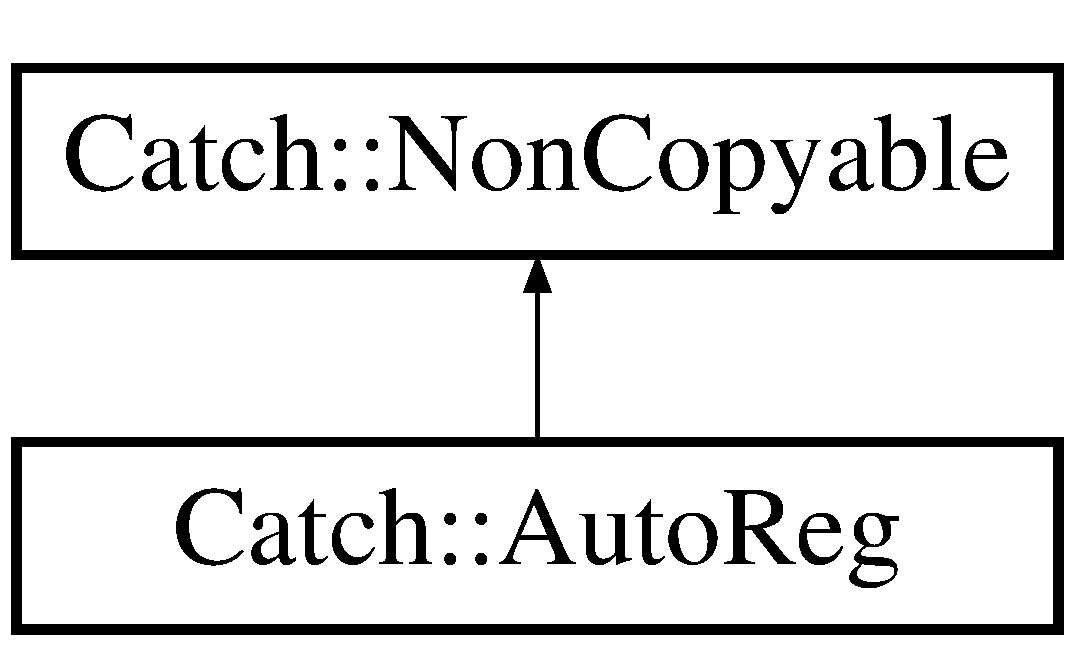
\includegraphics[height=2.000000cm]{struct_catch_1_1_auto_reg}
\end{center}
\end{figure}
\subsection*{Public Member Functions}
\begin{DoxyCompactItemize}
\item 
\mbox{\Hypertarget{struct_catch_1_1_auto_reg_a7eba02fb9d80b9896bf5a6517369af28}\label{struct_catch_1_1_auto_reg_a7eba02fb9d80b9896bf5a6517369af28}} 
{\bfseries Auto\+Reg} (\mbox{\hyperlink{struct_catch_1_1_i_test_invoker}{I\+Test\+Invoker}} $\ast$invoker, \mbox{\hyperlink{struct_catch_1_1_source_line_info}{Source\+Line\+Info}} const \&line\+Info, \mbox{\hyperlink{class_catch_1_1_string_ref}{String\+Ref}} const \&class\+Or\+Method, \mbox{\hyperlink{struct_catch_1_1_name_and_tags}{Name\+And\+Tags}} const \&name\+And\+Tags) noexcept
\end{DoxyCompactItemize}


The documentation for this struct was generated from the following file\+:\begin{DoxyCompactItemize}
\item 
D\+:/kouluhommat/\+Advanced Object-\/\+Oriented Programming/lopputyö/\+Battleship/\+Battleship/catch.\+hpp\end{DoxyCompactItemize}

\hypertarget{class_catch_1_1_benchmark_looper}{}\section{Catch\+:\+:Benchmark\+Looper Class Reference}
\label{class_catch_1_1_benchmark_looper}\index{Catch\+::\+Benchmark\+Looper@{Catch\+::\+Benchmark\+Looper}}


{\ttfamily \#include $<$catch.\+hpp$>$}

\subsection*{Public Member Functions}
\begin{DoxyCompactItemize}
\item 
\mbox{\hyperlink{class_catch_1_1_benchmark_looper_ab9ba6397306a70082f39e63a8a71bde6}{Benchmark\+Looper}} (\mbox{\hyperlink{class_catch_1_1_string_ref}{String\+Ref}} name)
\item 
\mbox{\hyperlink{class_catch_1_1_benchmark_looper_a54da41bada9da038dc05faf41d746765}{operator bool}} ()
\item 
void \mbox{\hyperlink{class_catch_1_1_benchmark_looper_a210552aff5b19408637444d4bb35d59c}{increment}} ()
\item 
void \mbox{\hyperlink{class_catch_1_1_benchmark_looper_a0697d1b266112b110edf2025b82c4e77}{report\+Start}} ()
\item 
auto \mbox{\hyperlink{class_catch_1_1_benchmark_looper_a97bd944521f519b1593a5d1d2f9998fa}{needs\+More\+Iterations}} () -\/$>$ bool
\end{DoxyCompactItemize}


\subsection{Constructor \& Destructor Documentation}
\mbox{\Hypertarget{class_catch_1_1_benchmark_looper_ab9ba6397306a70082f39e63a8a71bde6}\label{class_catch_1_1_benchmark_looper_ab9ba6397306a70082f39e63a8a71bde6}} 
\index{Catch\+::\+Benchmark\+Looper@{Catch\+::\+Benchmark\+Looper}!Benchmark\+Looper@{Benchmark\+Looper}}
\index{Benchmark\+Looper@{Benchmark\+Looper}!Catch\+::\+Benchmark\+Looper@{Catch\+::\+Benchmark\+Looper}}
\subsubsection{\texorpdfstring{Benchmark\+Looper()}{BenchmarkLooper()}}
{\footnotesize\ttfamily Catch\+::\+Benchmark\+Looper\+::\+Benchmark\+Looper (\begin{DoxyParamCaption}\item[{\mbox{\hyperlink{class_catch_1_1_string_ref}{String\+Ref}}}]{name }\end{DoxyParamCaption})\hspace{0.3cm}{\ttfamily [inline]}}



\subsection{Member Function Documentation}
\mbox{\Hypertarget{class_catch_1_1_benchmark_looper_a210552aff5b19408637444d4bb35d59c}\label{class_catch_1_1_benchmark_looper_a210552aff5b19408637444d4bb35d59c}} 
\index{Catch\+::\+Benchmark\+Looper@{Catch\+::\+Benchmark\+Looper}!increment@{increment}}
\index{increment@{increment}!Catch\+::\+Benchmark\+Looper@{Catch\+::\+Benchmark\+Looper}}
\subsubsection{\texorpdfstring{increment()}{increment()}}
{\footnotesize\ttfamily void Catch\+::\+Benchmark\+Looper\+::increment (\begin{DoxyParamCaption}{ }\end{DoxyParamCaption})\hspace{0.3cm}{\ttfamily [inline]}}

\mbox{\Hypertarget{class_catch_1_1_benchmark_looper_a97bd944521f519b1593a5d1d2f9998fa}\label{class_catch_1_1_benchmark_looper_a97bd944521f519b1593a5d1d2f9998fa}} 
\index{Catch\+::\+Benchmark\+Looper@{Catch\+::\+Benchmark\+Looper}!needs\+More\+Iterations@{needs\+More\+Iterations}}
\index{needs\+More\+Iterations@{needs\+More\+Iterations}!Catch\+::\+Benchmark\+Looper@{Catch\+::\+Benchmark\+Looper}}
\subsubsection{\texorpdfstring{needs\+More\+Iterations()}{needsMoreIterations()}}
{\footnotesize\ttfamily auto Catch\+::\+Benchmark\+Looper\+::needs\+More\+Iterations (\begin{DoxyParamCaption}{ }\end{DoxyParamCaption}) -\/$>$  bool}

\mbox{\Hypertarget{class_catch_1_1_benchmark_looper_a54da41bada9da038dc05faf41d746765}\label{class_catch_1_1_benchmark_looper_a54da41bada9da038dc05faf41d746765}} 
\index{Catch\+::\+Benchmark\+Looper@{Catch\+::\+Benchmark\+Looper}!operator bool@{operator bool}}
\index{operator bool@{operator bool}!Catch\+::\+Benchmark\+Looper@{Catch\+::\+Benchmark\+Looper}}
\subsubsection{\texorpdfstring{operator bool()}{operator bool()}}
{\footnotesize\ttfamily Catch\+::\+Benchmark\+Looper\+::operator bool (\begin{DoxyParamCaption}{ }\end{DoxyParamCaption})\hspace{0.3cm}{\ttfamily [inline]}, {\ttfamily [explicit]}}

\mbox{\Hypertarget{class_catch_1_1_benchmark_looper_a0697d1b266112b110edf2025b82c4e77}\label{class_catch_1_1_benchmark_looper_a0697d1b266112b110edf2025b82c4e77}} 
\index{Catch\+::\+Benchmark\+Looper@{Catch\+::\+Benchmark\+Looper}!report\+Start@{report\+Start}}
\index{report\+Start@{report\+Start}!Catch\+::\+Benchmark\+Looper@{Catch\+::\+Benchmark\+Looper}}
\subsubsection{\texorpdfstring{report\+Start()}{reportStart()}}
{\footnotesize\ttfamily void Catch\+::\+Benchmark\+Looper\+::report\+Start (\begin{DoxyParamCaption}{ }\end{DoxyParamCaption})}



The documentation for this class was generated from the following file\+:\begin{DoxyCompactItemize}
\item 
D\+:/kouluhommat/\+Advanced Object-\/\+Oriented Programming/lopputyö/\+Battleship/\+Battleship/\mbox{\hyperlink{catch_8hpp}{catch.\+hpp}}\end{DoxyCompactItemize}

\hypertarget{class_catch_1_1_binary_expr}{}\section{Catch\+:\+:Binary\+Expr$<$ LhsT, RhsT $>$ Class Template Reference}
\label{class_catch_1_1_binary_expr}\index{Catch\+::\+Binary\+Expr$<$ Lhs\+T, Rhs\+T $>$@{Catch\+::\+Binary\+Expr$<$ Lhs\+T, Rhs\+T $>$}}
Inheritance diagram for Catch\+:\+:Binary\+Expr$<$ LhsT, RhsT $>$\+:\begin{figure}[H]
\begin{center}
\leavevmode
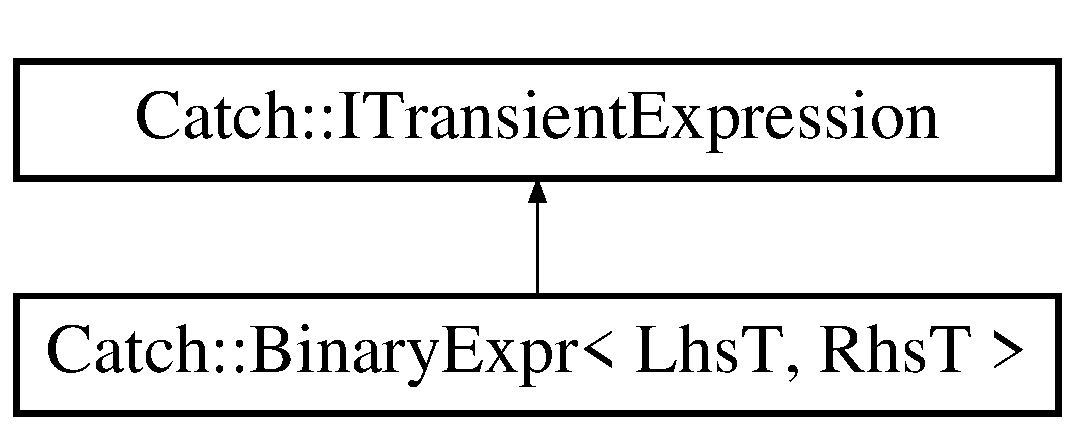
\includegraphics[height=2.000000cm]{class_catch_1_1_binary_expr}
\end{center}
\end{figure}
\subsection*{Public Member Functions}
\begin{DoxyCompactItemize}
\item 
\mbox{\Hypertarget{class_catch_1_1_binary_expr_a657d66346aef97a760c22776fe6008b6}\label{class_catch_1_1_binary_expr_a657d66346aef97a760c22776fe6008b6}} 
{\bfseries Binary\+Expr} (bool comparison\+Result, LhsT lhs, \mbox{\hyperlink{class_catch_1_1_string_ref}{String\+Ref}} op, RhsT rhs)
\end{DoxyCompactItemize}
\subsection*{Additional Inherited Members}


The documentation for this class was generated from the following file\+:\begin{DoxyCompactItemize}
\item 
D\+:/kouluhommat/\+Advanced Object-\/\+Oriented Programming/lopputyö/\+Battleship/\+Battleship/catch.\+hpp\end{DoxyCompactItemize}

\hypertarget{class_board}{}\section{Board Class Reference}
\label{class_board}\index{Board@{Board}}
\subsection*{Public Member Functions}
\begin{DoxyCompactItemize}
\item 
\mbox{\hyperlink{class_board_aa08d83943c9f7c727a96175feb05f1f8}{Board}} (const \mbox{\hyperlink{class_game}{Game}} \&g)
\begin{DoxyCompactList}\small\item\em Constructor for game board. \end{DoxyCompactList}\item 
\mbox{\hyperlink{class_board_af73f45730119a1fd8f6670f53f959e68}{$\sim$\+Board}} ()
\begin{DoxyCompactList}\small\item\em Destructor for board object. \end{DoxyCompactList}\item 
void \mbox{\hyperlink{class_board_af74f0d4b43e5aa3faea16d7c6407b05e}{clear}} ()
\begin{DoxyCompactList}\small\item\em Clears screen. \end{DoxyCompactList}\item 
void \mbox{\hyperlink{class_board_aaf09ad3613729ef00351f2c309e9b6cc}{block}} ()
\begin{DoxyCompactList}\small\item\em Blocks cells. \end{DoxyCompactList}\item 
void \mbox{\hyperlink{class_board_afb89d8a0417a53952ee2b64437282253}{unblock}} ()
\begin{DoxyCompactList}\small\item\em Unblocks cells. \end{DoxyCompactList}\item 
void \mbox{\hyperlink{class_board_a47f5e3908bd99b9cf1a9ed2050b7cfd9}{display}} (bool show\+Shots) const
\begin{DoxyCompactList}\small\item\em Displays the board. \end{DoxyCompactList}\item 
bool \mbox{\hyperlink{class_board_a47be427a7c565e29dd2606c95972bf91}{place\+Ship}} (\mbox{\hyperlink{class_point}{Point}} tl, int ship\+ID, \mbox{\hyperlink{_globals_8h_a224b9163917ac32fc95a60d8c1eec3aa}{Direction}} d)
\begin{DoxyCompactList}\small\item\em Places ships on game board. \end{DoxyCompactList}\item 
bool \mbox{\hyperlink{class_board_a7d2f52e12bb4c861a1484ec0f54897d0}{remove\+Ship}} (\mbox{\hyperlink{class_point}{Point}} tl, int ship\+ID, \mbox{\hyperlink{_globals_8h_a224b9163917ac32fc95a60d8c1eec3aa}{Direction}} d)
\begin{DoxyCompactList}\small\item\em Removes ships from board. \end{DoxyCompactList}\item 
bool \mbox{\hyperlink{class_board_aad9932b230d16c6eef6fd9305399fbd2}{attack}} (\mbox{\hyperlink{class_point}{Point}} p, bool \&hit, bool \&destroyed, int \&ship\+ID)
\begin{DoxyCompactList}\small\item\em Attacks target cell. \end{DoxyCompactList}\item 
bool \mbox{\hyperlink{class_board_a4653d3028e70fea9f56523173a2e0a13}{all\+Destroyed}} () const
\item 
\mbox{\Hypertarget{class_board_a1b25abe81ff08e6b574ecfc2dcaaa5be}\label{class_board_a1b25abe81ff08e6b574ecfc2dcaaa5be}} 
\mbox{\hyperlink{class_board_a1b25abe81ff08e6b574ecfc2dcaaa5be}{Board}} (const \mbox{\hyperlink{class_board}{Board}} \&)=delete
\begin{DoxyCompactList}\small\item\em Prevents board object from being copied/assigned. \end{DoxyCompactList}\item 
\mbox{\Hypertarget{class_board_a892306c4b944bfe904b297092763084a}\label{class_board_a892306c4b944bfe904b297092763084a}} 
\mbox{\hyperlink{class_board}{Board}} \& {\bfseries operator=} (const \mbox{\hyperlink{class_board}{Board}} \&)=delete
\end{DoxyCompactItemize}


\subsection{Constructor \& Destructor Documentation}
\mbox{\Hypertarget{class_board_aa08d83943c9f7c727a96175feb05f1f8}\label{class_board_aa08d83943c9f7c727a96175feb05f1f8}} 
\index{Board@{Board}!Board@{Board}}
\index{Board@{Board}!Board@{Board}}
\subsubsection{\texorpdfstring{Board()}{Board()}}
{\footnotesize\ttfamily Board\+::\+Board (\begin{DoxyParamCaption}\item[{const \mbox{\hyperlink{class_game}{Game}} \&}]{g }\end{DoxyParamCaption})}



Constructor for game board. 

Delegates to board implementation 
\begin{DoxyParams}{Parameters}
{\em g} & reference to game object \\
\hline
\end{DoxyParams}
\mbox{\Hypertarget{class_board_af73f45730119a1fd8f6670f53f959e68}\label{class_board_af73f45730119a1fd8f6670f53f959e68}} 
\index{Board@{Board}!````~Board@{$\sim$\+Board}}
\index{````~Board@{$\sim$\+Board}!Board@{Board}}
\subsubsection{\texorpdfstring{$\sim$\+Board()}{~Board()}}
{\footnotesize\ttfamily Board\+::$\sim$\+Board (\begin{DoxyParamCaption}{ }\end{DoxyParamCaption})}



Destructor for board object. 

Deletes board implementation 

\subsection{Member Function Documentation}
\mbox{\Hypertarget{class_board_a4653d3028e70fea9f56523173a2e0a13}\label{class_board_a4653d3028e70fea9f56523173a2e0a13}} 
\index{Board@{Board}!all\+Destroyed@{all\+Destroyed}}
\index{all\+Destroyed@{all\+Destroyed}!Board@{Board}}
\subsubsection{\texorpdfstring{all\+Destroyed()}{allDestroyed()}}
{\footnotesize\ttfamily bool Board\+::all\+Destroyed (\begin{DoxyParamCaption}{ }\end{DoxyParamCaption}) const}

Checks if all ships are destroyed

Delegates to board implementation\textquotesingle{}s all\+Destroyed method \mbox{\Hypertarget{class_board_aad9932b230d16c6eef6fd9305399fbd2}\label{class_board_aad9932b230d16c6eef6fd9305399fbd2}} 
\index{Board@{Board}!attack@{attack}}
\index{attack@{attack}!Board@{Board}}
\subsubsection{\texorpdfstring{attack()}{attack()}}
{\footnotesize\ttfamily bool Board\+::attack (\begin{DoxyParamCaption}\item[{\mbox{\hyperlink{class_point}{Point}}}]{p,  }\item[{bool \&}]{hit,  }\item[{bool \&}]{destroyed,  }\item[{int \&}]{ship\+ID }\end{DoxyParamCaption})}



Attacks target cell. 

Delegates to board implementation\textquotesingle{}s attack method 
\begin{DoxyParams}{Parameters}
{\em p} & \mbox{\hyperlink{class_point}{Point}} that has the targeted cell \\
\hline
{\em hit} & reference to boolean which indicates if ship was hit \\
\hline
{\em destroyed} & reference to boolean which indicates if ship was destroyed \\
\hline
{\em ship\+ID} & reference to integer which returns ID of ship that was hit \\
\hline
\end{DoxyParams}
\mbox{\Hypertarget{class_board_aaf09ad3613729ef00351f2c309e9b6cc}\label{class_board_aaf09ad3613729ef00351f2c309e9b6cc}} 
\index{Board@{Board}!block@{block}}
\index{block@{block}!Board@{Board}}
\subsubsection{\texorpdfstring{block()}{block()}}
{\footnotesize\ttfamily void Board\+::block (\begin{DoxyParamCaption}{ }\end{DoxyParamCaption})}



Blocks cells. 

Delegates to board implementation\textquotesingle{}s block method \mbox{\Hypertarget{class_board_af74f0d4b43e5aa3faea16d7c6407b05e}\label{class_board_af74f0d4b43e5aa3faea16d7c6407b05e}} 
\index{Board@{Board}!clear@{clear}}
\index{clear@{clear}!Board@{Board}}
\subsubsection{\texorpdfstring{clear()}{clear()}}
{\footnotesize\ttfamily void Board\+::clear (\begin{DoxyParamCaption}{ }\end{DoxyParamCaption})}



Clears screen. 

Delegates to board implementation\textquotesingle{}s clear method \mbox{\Hypertarget{class_board_a47f5e3908bd99b9cf1a9ed2050b7cfd9}\label{class_board_a47f5e3908bd99b9cf1a9ed2050b7cfd9}} 
\index{Board@{Board}!display@{display}}
\index{display@{display}!Board@{Board}}
\subsubsection{\texorpdfstring{display()}{display()}}
{\footnotesize\ttfamily void Board\+::display (\begin{DoxyParamCaption}\item[{bool}]{show\+Shots }\end{DoxyParamCaption}) const}



Displays the board. 

Delegates to board implementation\textquotesingle{}s display method 
\begin{DoxyParams}{Parameters}
{\em show\+Shots} & boolean for showing shots \\
\hline
\end{DoxyParams}
\mbox{\Hypertarget{class_board_a47be427a7c565e29dd2606c95972bf91}\label{class_board_a47be427a7c565e29dd2606c95972bf91}} 
\index{Board@{Board}!place\+Ship@{place\+Ship}}
\index{place\+Ship@{place\+Ship}!Board@{Board}}
\subsubsection{\texorpdfstring{place\+Ship()}{placeShip()}}
{\footnotesize\ttfamily bool Board\+::place\+Ship (\begin{DoxyParamCaption}\item[{\mbox{\hyperlink{class_point}{Point}}}]{tl,  }\item[{int}]{ship\+ID,  }\item[{\mbox{\hyperlink{_globals_8h_a224b9163917ac32fc95a60d8c1eec3aa}{Direction}}}]{d }\end{DoxyParamCaption})}



Places ships on game board. 

Delegates to board implementation\textquotesingle{}s place\+Ship method 
\begin{DoxyParams}{Parameters}
{\em tl} & \mbox{\hyperlink{class_point}{Point}} containing top left cell \\
\hline
{\em ship\+ID} & integer for ship id \\
\hline
{\em d} & Direction the ship is facing \\
\hline
\end{DoxyParams}
\mbox{\Hypertarget{class_board_a7d2f52e12bb4c861a1484ec0f54897d0}\label{class_board_a7d2f52e12bb4c861a1484ec0f54897d0}} 
\index{Board@{Board}!remove\+Ship@{remove\+Ship}}
\index{remove\+Ship@{remove\+Ship}!Board@{Board}}
\subsubsection{\texorpdfstring{remove\+Ship()}{removeShip()}}
{\footnotesize\ttfamily bool Board\+::remove\+Ship (\begin{DoxyParamCaption}\item[{\mbox{\hyperlink{class_point}{Point}}}]{tl,  }\item[{int}]{ship\+ID,  }\item[{\mbox{\hyperlink{_globals_8h_a224b9163917ac32fc95a60d8c1eec3aa}{Direction}}}]{d }\end{DoxyParamCaption})}



Removes ships from board. 

Delegates to board implementation\textquotesingle{}s remove\+Ship method 
\begin{DoxyParams}{Parameters}
{\em tl} & \mbox{\hyperlink{class_point}{Point}} containing top left cell \\
\hline
{\em ship\+ID} & integer for ship id \\
\hline
{\em d} & Direction the ship is facing \\
\hline
\end{DoxyParams}
\mbox{\Hypertarget{class_board_afb89d8a0417a53952ee2b64437282253}\label{class_board_afb89d8a0417a53952ee2b64437282253}} 
\index{Board@{Board}!unblock@{unblock}}
\index{unblock@{unblock}!Board@{Board}}
\subsubsection{\texorpdfstring{unblock()}{unblock()}}
{\footnotesize\ttfamily void Board\+::unblock (\begin{DoxyParamCaption}{ }\end{DoxyParamCaption})}



Unblocks cells. 

Delegates to board implementation\textquotesingle{}s unblock method 

The documentation for this class was generated from the following files\+:\begin{DoxyCompactItemize}
\item 
D\+:/kouluhommat/\+Advanced Object-\/\+Oriented Programming/lopputyö/\+Battleship/\+Battleship/\mbox{\hyperlink{_board_8h}{Board.\+h}}\item 
D\+:/kouluhommat/\+Advanced Object-\/\+Oriented Programming/lopputyö/\+Battleship/\+Battleship/\mbox{\hyperlink{_board_8cpp}{Board.\+cpp}}\end{DoxyCompactItemize}

\hypertarget{class_board_impl}{}\section{Board\+Impl Class Reference}
\label{class_board_impl}\index{Board\+Impl@{Board\+Impl}}


{\ttfamily \#include $<$Board.\+h$>$}

\subsection*{Public Member Functions}
\begin{DoxyCompactItemize}
\item 
\mbox{\hyperlink{class_board_impl_a2c3f1cce7def17781c0025d1e68d0af5}{Board\+Impl}} (const \mbox{\hyperlink{class_game}{Game}} \&g)
\item 
void \mbox{\hyperlink{class_board_impl_a47c7733ed5ec7a09fe9710f443fe0952}{clear}} ()
\item 
void \mbox{\hyperlink{class_board_impl_abd7743ed758876c2855b2bb7474cf2eb}{block}} ()
\item 
void \mbox{\hyperlink{class_board_impl_a36defeb0096154a4606442da9122c810}{unblock}} ()
\item 
void \mbox{\hyperlink{class_board_impl_a4b600b257cfe79f10ac8792ab69eb388}{display}} (bool show\+Shots) const
\item 
bool \mbox{\hyperlink{class_board_impl_af0fd0226fc1f401374a0cbbfbab98769}{place\+Ship}} (\mbox{\hyperlink{class_point}{Point}} tl, int ship\+ID, \mbox{\hyperlink{_globals_8h_a224b9163917ac32fc95a60d8c1eec3aa}{Direction}} d)
\item 
bool \mbox{\hyperlink{class_board_impl_a8573ccd5fb2a837f324cc0f190cece5d}{remove\+Ship}} (\mbox{\hyperlink{class_point}{Point}} tl, int ship\+ID, \mbox{\hyperlink{_globals_8h_a224b9163917ac32fc95a60d8c1eec3aa}{Direction}} d)
\item 
bool \mbox{\hyperlink{class_board_impl_afd58266f5c81679fef78c0d1abb9d0d5}{attack}} (\mbox{\hyperlink{class_point}{Point}} p, bool \&hit, bool \&destroyed, int \&ship\+ID)
\item 
bool \mbox{\hyperlink{class_board_impl_a00ae397df7ab1a47868078a2e0ec54b8}{all\+Destroyed}} () const
\end{DoxyCompactItemize}


\subsection{Detailed Description}
\mbox{\hyperlink{class_board_impl}{Board\+Impl}}\+: class for board implementation 

\subsection{Constructor \& Destructor Documentation}
\mbox{\Hypertarget{class_board_impl_a2c3f1cce7def17781c0025d1e68d0af5}\label{class_board_impl_a2c3f1cce7def17781c0025d1e68d0af5}} 
\index{Board\+Impl@{Board\+Impl}!Board\+Impl@{Board\+Impl}}
\index{Board\+Impl@{Board\+Impl}!Board\+Impl@{Board\+Impl}}
\subsubsection{\texorpdfstring{Board\+Impl()}{BoardImpl()}}
{\footnotesize\ttfamily Board\+Impl\+::\+Board\+Impl (\begin{DoxyParamCaption}\item[{const \mbox{\hyperlink{class_game}{Game}} \&}]{g }\end{DoxyParamCaption})}

\mbox{\hyperlink{class_board_impl}{Board\+Impl}} constructor 
\begin{DoxyParams}{Parameters}
{\em g} & reference to game object Loops through rows and columns and fills them with \textquotesingle{}.\textquotesingle{} \\
\hline
\end{DoxyParams}


\subsection{Member Function Documentation}
\mbox{\Hypertarget{class_board_impl_a00ae397df7ab1a47868078a2e0ec54b8}\label{class_board_impl_a00ae397df7ab1a47868078a2e0ec54b8}} 
\index{Board\+Impl@{Board\+Impl}!all\+Destroyed@{all\+Destroyed}}
\index{all\+Destroyed@{all\+Destroyed}!Board\+Impl@{Board\+Impl}}
\subsubsection{\texorpdfstring{all\+Destroyed()}{allDestroyed()}}
{\footnotesize\ttfamily bool Board\+Impl\+::all\+Destroyed (\begin{DoxyParamCaption}{ }\end{DoxyParamCaption}) const}

Method for checking if all ships have been destroyed Loops through rows and columns

Checks if board contains other symbols than \textquotesingle{}X\textquotesingle{}, \textquotesingle{}.\textquotesingle{} or \textquotesingle{}o\textquotesingle{} If yes, then there are still ships left\mbox{\Hypertarget{class_board_impl_afd58266f5c81679fef78c0d1abb9d0d5}\label{class_board_impl_afd58266f5c81679fef78c0d1abb9d0d5}} 
\index{Board\+Impl@{Board\+Impl}!attack@{attack}}
\index{attack@{attack}!Board\+Impl@{Board\+Impl}}
\subsubsection{\texorpdfstring{attack()}{attack()}}
{\footnotesize\ttfamily bool Board\+Impl\+::attack (\begin{DoxyParamCaption}\item[{\mbox{\hyperlink{class_point}{Point}}}]{p,  }\item[{bool \&}]{hit,  }\item[{bool \&}]{destroyed,  }\item[{int \&}]{ship\+ID }\end{DoxyParamCaption})}

Method for shooting on a cell 
\begin{DoxyParams}{Parameters}
{\em p} & \mbox{\hyperlink{class_point}{Point}} that has the cell \\
\hline
{\em hit} & reference to boolean which indicates if ship was hit \\
\hline
{\em destroyed} & reference to boolean which indicates if ship was destroyed \\
\hline
{\em ship\+ID} & reference to integer which returns ID of ship that was hit \\
\hline
\end{DoxyParams}
Returns false if target is out of bounds

Returns false if target has already been shot

Checks if it\textquotesingle{}s possible to attack target cell

Checks if target doesn\textquotesingle{}t have a dot on it

Updates array with hit mark

Checks if ship exists

Checks if ship doesn\textquotesingle{}t exist, it has been sunk

Loop that finds the right ship

$<$ If hit was a miss \mbox{\Hypertarget{class_board_impl_abd7743ed758876c2855b2bb7474cf2eb}\label{class_board_impl_abd7743ed758876c2855b2bb7474cf2eb}} 
\index{Board\+Impl@{Board\+Impl}!block@{block}}
\index{block@{block}!Board\+Impl@{Board\+Impl}}
\subsubsection{\texorpdfstring{block()}{block()}}
{\footnotesize\ttfamily void Board\+Impl\+::block (\begin{DoxyParamCaption}{ }\end{DoxyParamCaption})}

Method for blocking cells loops through game\textquotesingle{}s rows and columns and blocks them with \textquotesingle{}\#\textquotesingle{} symbol with 50\% chance \mbox{\Hypertarget{class_board_impl_a47c7733ed5ec7a09fe9710f443fe0952}\label{class_board_impl_a47c7733ed5ec7a09fe9710f443fe0952}} 
\index{Board\+Impl@{Board\+Impl}!clear@{clear}}
\index{clear@{clear}!Board\+Impl@{Board\+Impl}}
\subsubsection{\texorpdfstring{clear()}{clear()}}
{\footnotesize\ttfamily void Board\+Impl\+::clear (\begin{DoxyParamCaption}{ }\end{DoxyParamCaption})}

Method for clearing the game screen Loops through rows and columns and fills them with \textquotesingle{}.\textquotesingle{} \mbox{\Hypertarget{class_board_impl_a4b600b257cfe79f10ac8792ab69eb388}\label{class_board_impl_a4b600b257cfe79f10ac8792ab69eb388}} 
\index{Board\+Impl@{Board\+Impl}!display@{display}}
\index{display@{display}!Board\+Impl@{Board\+Impl}}
\subsubsection{\texorpdfstring{display()}{display()}}
{\footnotesize\ttfamily void Board\+Impl\+::display (\begin{DoxyParamCaption}\item[{bool}]{show\+Shots }\end{DoxyParamCaption}) const}

Display method for showing game screen 
\begin{DoxyParams}{Parameters}
{\em show\+Shots} & boolean to check if shots are visible or not \\
\hline
\end{DoxyParams}
$<$ Empty spaces to line header numbers with cells ~\newline
~\newline
~\newline
~\newline
~\newline
~\newline
~\newline
~\newline
~\newline
 Loops through columns to create line with header (numbers)

Loops through rows

$<$ Creates header numbers for columns

Checks if shots are visible

Checks if cells don\textquotesingle{}t contain \textquotesingle{}X\textquotesingle{} and \textquotesingle{}o\textquotesingle{} and if cells contain alphabetic character

$<$ If cell is alphabetic, turns it into \textquotesingle{}.\textquotesingle{}

$<$ If cell is not alphabetic or contains \textquotesingle{}X\textquotesingle{} or \textquotesingle{}o\textquotesingle{}

Prints the cell

$<$ If show\+Shots is false it prints the cell \mbox{\Hypertarget{class_board_impl_af0fd0226fc1f401374a0cbbfbab98769}\label{class_board_impl_af0fd0226fc1f401374a0cbbfbab98769}} 
\index{Board\+Impl@{Board\+Impl}!place\+Ship@{place\+Ship}}
\index{place\+Ship@{place\+Ship}!Board\+Impl@{Board\+Impl}}
\subsubsection{\texorpdfstring{place\+Ship()}{placeShip()}}
{\footnotesize\ttfamily bool Board\+Impl\+::place\+Ship (\begin{DoxyParamCaption}\item[{\mbox{\hyperlink{class_point}{Point}}}]{tl,  }\item[{int}]{ship\+ID,  }\item[{\mbox{\hyperlink{_globals_8h_a224b9163917ac32fc95a60d8c1eec3aa}{Direction}}}]{d }\end{DoxyParamCaption})}

Method for placing a ship on cell 
\begin{DoxyParams}{Parameters}
{\em tl} & \mbox{\hyperlink{class_point}{Point}} for top left cell \\
\hline
{\em ship\+ID} & integer used as ship\textquotesingle{}s ID \\
\hline
{\em d} & Direction where the ship is facing \\
\hline
\end{DoxyParams}
$<$ Boolean for checking if ship placement is valid

Checks if ID is invalid

Checks if cell is outside of board

Checks if ship extends outside of board

Checks if ship has been placed before

Checks if ship overlaps another one

Places ship on game board only if ship placement is valid \mbox{\Hypertarget{class_board_impl_a8573ccd5fb2a837f324cc0f190cece5d}\label{class_board_impl_a8573ccd5fb2a837f324cc0f190cece5d}} 
\index{Board\+Impl@{Board\+Impl}!remove\+Ship@{remove\+Ship}}
\index{remove\+Ship@{remove\+Ship}!Board\+Impl@{Board\+Impl}}
\subsubsection{\texorpdfstring{remove\+Ship()}{removeShip()}}
{\footnotesize\ttfamily bool Board\+Impl\+::remove\+Ship (\begin{DoxyParamCaption}\item[{\mbox{\hyperlink{class_point}{Point}}}]{tl,  }\item[{int}]{ship\+ID,  }\item[{\mbox{\hyperlink{_globals_8h_a224b9163917ac32fc95a60d8c1eec3aa}{Direction}}}]{d }\end{DoxyParamCaption})}

Method for taking a ship away from the grid 
\begin{DoxyParams}{Parameters}
{\em tl} & \mbox{\hyperlink{class_point}{Point}} for top left cell \\
\hline
{\em ship\+ID} & integer used as ship\textquotesingle{}s ID \\
\hline
{\em d} & Direction where the ship is facing \\
\hline
\end{DoxyParams}
Checks if ID is invalid

Checks if ship is there

Clears the cell if ship is there \mbox{\Hypertarget{class_board_impl_a36defeb0096154a4606442da9122c810}\label{class_board_impl_a36defeb0096154a4606442da9122c810}} 
\index{Board\+Impl@{Board\+Impl}!unblock@{unblock}}
\index{unblock@{unblock}!Board\+Impl@{Board\+Impl}}
\subsubsection{\texorpdfstring{unblock()}{unblock()}}
{\footnotesize\ttfamily void Board\+Impl\+::unblock (\begin{DoxyParamCaption}{ }\end{DoxyParamCaption})}

Method for unblocking cells loops through game\textquotesingle{}s rows and columns and replaces \textquotesingle{}\#\textquotesingle{} with \textquotesingle{}.\textquotesingle{} 

The documentation for this class was generated from the following files\+:\begin{DoxyCompactItemize}
\item 
D\+:/kouluhommat/\+Advanced Object-\/\+Oriented Programming/lopputyö/\+Battleship/\+Battleship/\mbox{\hyperlink{_board_8h}{Board.\+h}}\item 
D\+:/kouluhommat/\+Advanced Object-\/\+Oriented Programming/lopputyö/\+Battleship/\+Battleship/\mbox{\hyperlink{_board_impl_8cpp}{Board\+Impl.\+cpp}}\end{DoxyCompactItemize}

\hypertarget{class_catch_1_1_capturer}{}\section{Catch\+:\+:Capturer Class Reference}
\label{class_catch_1_1_capturer}\index{Catch\+::\+Capturer@{Catch\+::\+Capturer}}
\subsection*{Public Member Functions}
\begin{DoxyCompactItemize}
\item 
\mbox{\Hypertarget{class_catch_1_1_capturer_a86b0b27acc803a4e1310c10820f3038f}\label{class_catch_1_1_capturer_a86b0b27acc803a4e1310c10820f3038f}} 
{\bfseries Capturer} (\mbox{\hyperlink{class_catch_1_1_string_ref}{String\+Ref}} macro\+Name, \mbox{\hyperlink{struct_catch_1_1_source_line_info}{Source\+Line\+Info}} const \&line\+Info, Result\+Was\+::\+Of\+Type result\+Type, \mbox{\hyperlink{class_catch_1_1_string_ref}{String\+Ref}} names)
\item 
\mbox{\Hypertarget{class_catch_1_1_capturer_a0695ebf77f7cdcb344c73bcb3d9131e4}\label{class_catch_1_1_capturer_a0695ebf77f7cdcb344c73bcb3d9131e4}} 
void {\bfseries capture\+Value} (size\+\_\+t index, std\+::string const \&value)
\item 
\mbox{\Hypertarget{class_catch_1_1_capturer_a60d08e6db2e54740bb2298bbbec3bc0b}\label{class_catch_1_1_capturer_a60d08e6db2e54740bb2298bbbec3bc0b}} 
{\footnotesize template$<$typename T $>$ }\\void {\bfseries capture\+Values} (size\+\_\+t index, T const \&value)
\item 
\mbox{\Hypertarget{class_catch_1_1_capturer_a76f2a097cfeb3042688300b81eb9bcbc}\label{class_catch_1_1_capturer_a76f2a097cfeb3042688300b81eb9bcbc}} 
{\footnotesize template$<$typename T , typename... Ts$>$ }\\void {\bfseries capture\+Values} (size\+\_\+t index, T const \&value, Ts const \&... values)
\end{DoxyCompactItemize}


The documentation for this class was generated from the following file\+:\begin{DoxyCompactItemize}
\item 
D\+:/kouluhommat/\+Advanced Object-\/\+Oriented Programming/lopputyö/\+Battleship/\+Battleship/catch.\+hpp\end{DoxyCompactItemize}

\hypertarget{struct_catch_1_1_matchers_1_1_std_string_1_1_cased_string}{}\section{Catch\+:\+:Matchers\+:\+:Std\+String\+:\+:Cased\+String Struct Reference}
\label{struct_catch_1_1_matchers_1_1_std_string_1_1_cased_string}\index{Catch\+::\+Matchers\+::\+Std\+String\+::\+Cased\+String@{Catch\+::\+Matchers\+::\+Std\+String\+::\+Cased\+String}}
\subsection*{Public Member Functions}
\begin{DoxyCompactItemize}
\item 
\mbox{\Hypertarget{struct_catch_1_1_matchers_1_1_std_string_1_1_cased_string_aa88bbc5acd2bff22351d8d4b1816b561}\label{struct_catch_1_1_matchers_1_1_std_string_1_1_cased_string_aa88bbc5acd2bff22351d8d4b1816b561}} 
{\bfseries Cased\+String} (std\+::string const \&str, Case\+Sensitive\+::\+Choice case\+Sensitivity)
\item 
\mbox{\Hypertarget{struct_catch_1_1_matchers_1_1_std_string_1_1_cased_string_a77639b1165c01f424ee0e96f53335010}\label{struct_catch_1_1_matchers_1_1_std_string_1_1_cased_string_a77639b1165c01f424ee0e96f53335010}} 
std\+::string {\bfseries adjust\+String} (std\+::string const \&str) const
\item 
\mbox{\Hypertarget{struct_catch_1_1_matchers_1_1_std_string_1_1_cased_string_a9759155344d696b2476d764a1d95fcc9}\label{struct_catch_1_1_matchers_1_1_std_string_1_1_cased_string_a9759155344d696b2476d764a1d95fcc9}} 
std\+::string {\bfseries case\+Sensitivity\+Suffix} () const
\end{DoxyCompactItemize}
\subsection*{Public Attributes}
\begin{DoxyCompactItemize}
\item 
\mbox{\Hypertarget{struct_catch_1_1_matchers_1_1_std_string_1_1_cased_string_ae1c2864c986941536a6e94cca0528f92}\label{struct_catch_1_1_matchers_1_1_std_string_1_1_cased_string_ae1c2864c986941536a6e94cca0528f92}} 
Case\+Sensitive\+::\+Choice {\bfseries m\+\_\+case\+Sensitivity}
\item 
\mbox{\Hypertarget{struct_catch_1_1_matchers_1_1_std_string_1_1_cased_string_ad05dbc99aba3c3c386d6b856b213f911}\label{struct_catch_1_1_matchers_1_1_std_string_1_1_cased_string_ad05dbc99aba3c3c386d6b856b213f911}} 
std\+::string {\bfseries m\+\_\+str}
\end{DoxyCompactItemize}


The documentation for this struct was generated from the following file\+:\begin{DoxyCompactItemize}
\item 
D\+:/kouluhommat/\+Advanced Object-\/\+Oriented Programming/lopputyö/\+Battleship/\+Battleship/catch.\+hpp\end{DoxyCompactItemize}

\hypertarget{struct_catch_1_1_case_sensitive}{}\section{Catch\+:\+:Case\+Sensitive Struct Reference}
\label{struct_catch_1_1_case_sensitive}\index{Catch\+::\+Case\+Sensitive@{Catch\+::\+Case\+Sensitive}}
\subsection*{Public Types}
\begin{DoxyCompactItemize}
\item 
\mbox{\Hypertarget{struct_catch_1_1_case_sensitive_aad49d3aee2d97066642fffa919685c6a}\label{struct_catch_1_1_case_sensitive_aad49d3aee2d97066642fffa919685c6a}} 
enum {\bfseries Choice} \{ {\bfseries Yes}, 
{\bfseries No}
 \}
\end{DoxyCompactItemize}


The documentation for this struct was generated from the following file\+:\begin{DoxyCompactItemize}
\item 
D\+:/kouluhommat/\+Advanced Object-\/\+Oriented Programming/lopputyö/\+Battleship/\+Battleship/catch.\+hpp\end{DoxyCompactItemize}

\hypertarget{struct_catch__global__namespace__dummy}{}\section{Catch\+\_\+global\+\_\+namespace\+\_\+dummy Struct Reference}
\label{struct_catch__global__namespace__dummy}\index{Catch\+\_\+global\+\_\+namespace\+\_\+dummy@{Catch\+\_\+global\+\_\+namespace\+\_\+dummy}}


{\ttfamily \#include $<$catch.\+hpp$>$}



The documentation for this struct was generated from the following file\+:\begin{DoxyCompactItemize}
\item 
D\+:/kouluhommat/\+Advanced Object-\/\+Oriented Programming/lopputyö/\+Battleship/\+Battleship/\mbox{\hyperlink{catch_8hpp}{catch.\+hpp}}\end{DoxyCompactItemize}

\hypertarget{struct_catch_1_1_matchers_1_1_vector_1_1_contains_element_matcher}{}\section{Catch\+:\+:Matchers\+:\+:Vector\+:\+:Contains\+Element\+Matcher$<$ T $>$ Struct Template Reference}
\label{struct_catch_1_1_matchers_1_1_vector_1_1_contains_element_matcher}\index{Catch\+::\+Matchers\+::\+Vector\+::\+Contains\+Element\+Matcher$<$ T $>$@{Catch\+::\+Matchers\+::\+Vector\+::\+Contains\+Element\+Matcher$<$ T $>$}}
Inheritance diagram for Catch\+:\+:Matchers\+:\+:Vector\+:\+:Contains\+Element\+Matcher$<$ T $>$\+:\begin{figure}[H]
\begin{center}
\leavevmode
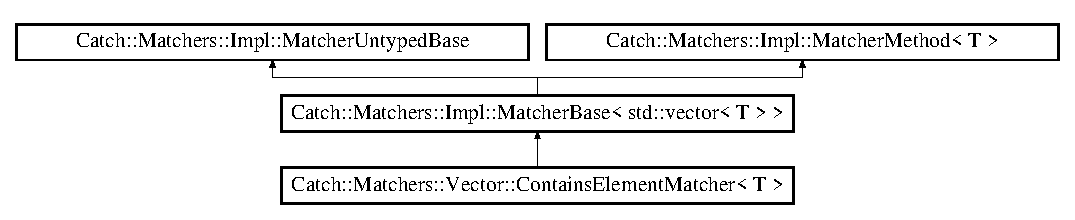
\includegraphics[height=2.514970cm]{struct_catch_1_1_matchers_1_1_vector_1_1_contains_element_matcher}
\end{center}
\end{figure}
\subsection*{Public Member Functions}
\begin{DoxyCompactItemize}
\item 
\mbox{\Hypertarget{struct_catch_1_1_matchers_1_1_vector_1_1_contains_element_matcher_a6a05740b5d3f89fac8de84ac0cff7b93}\label{struct_catch_1_1_matchers_1_1_vector_1_1_contains_element_matcher_a6a05740b5d3f89fac8de84ac0cff7b93}} 
{\bfseries Contains\+Element\+Matcher} (T const \&comparator)
\item 
\mbox{\Hypertarget{struct_catch_1_1_matchers_1_1_vector_1_1_contains_element_matcher_a6a4be6e5642e267433d370649beb0fac}\label{struct_catch_1_1_matchers_1_1_vector_1_1_contains_element_matcher_a6a4be6e5642e267433d370649beb0fac}} 
bool {\bfseries match} (std\+::vector$<$ T $>$ const \&v) const override
\item 
\mbox{\Hypertarget{struct_catch_1_1_matchers_1_1_vector_1_1_contains_element_matcher_aea3b674389a0afd82af6ba4b10f86ae6}\label{struct_catch_1_1_matchers_1_1_vector_1_1_contains_element_matcher_aea3b674389a0afd82af6ba4b10f86ae6}} 
std\+::string {\bfseries describe} () const override
\end{DoxyCompactItemize}
\subsection*{Public Attributes}
\begin{DoxyCompactItemize}
\item 
\mbox{\Hypertarget{struct_catch_1_1_matchers_1_1_vector_1_1_contains_element_matcher_ab7eada6c4bbce1d21b44773262f9cb23}\label{struct_catch_1_1_matchers_1_1_vector_1_1_contains_element_matcher_ab7eada6c4bbce1d21b44773262f9cb23}} 
T const  \& {\bfseries m\+\_\+comparator}
\end{DoxyCompactItemize}
\subsection*{Additional Inherited Members}


The documentation for this struct was generated from the following file\+:\begin{DoxyCompactItemize}
\item 
D\+:/kouluhommat/\+Advanced Object-\/\+Oriented Programming/lopputyö/\+Battleship/\+Battleship/catch.\+hpp\end{DoxyCompactItemize}

\hypertarget{struct_catch_1_1_matchers_1_1_std_string_1_1_contains_matcher}{}\section{Catch\+:\+:Matchers\+:\+:Std\+String\+:\+:Contains\+Matcher Struct Reference}
\label{struct_catch_1_1_matchers_1_1_std_string_1_1_contains_matcher}\index{Catch\+::\+Matchers\+::\+Std\+String\+::\+Contains\+Matcher@{Catch\+::\+Matchers\+::\+Std\+String\+::\+Contains\+Matcher}}
Inheritance diagram for Catch\+:\+:Matchers\+:\+:Std\+String\+:\+:Contains\+Matcher\+:\begin{figure}[H]
\begin{center}
\leavevmode
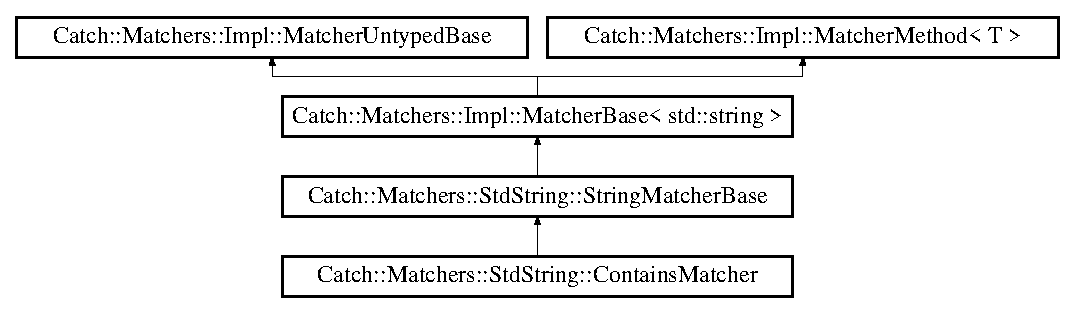
\includegraphics[height=3.758389cm]{struct_catch_1_1_matchers_1_1_std_string_1_1_contains_matcher}
\end{center}
\end{figure}
\subsection*{Public Member Functions}
\begin{DoxyCompactItemize}
\item 
\mbox{\Hypertarget{struct_catch_1_1_matchers_1_1_std_string_1_1_contains_matcher_acc892883c8409e34b28c9b39d4ef1fe3}\label{struct_catch_1_1_matchers_1_1_std_string_1_1_contains_matcher_acc892883c8409e34b28c9b39d4ef1fe3}} 
{\bfseries Contains\+Matcher} (\mbox{\hyperlink{struct_catch_1_1_matchers_1_1_std_string_1_1_cased_string}{Cased\+String}} const \&comparator)
\item 
\mbox{\Hypertarget{struct_catch_1_1_matchers_1_1_std_string_1_1_contains_matcher_a630628b234b037be83fe587081a80b53}\label{struct_catch_1_1_matchers_1_1_std_string_1_1_contains_matcher_a630628b234b037be83fe587081a80b53}} 
bool {\bfseries match} (std\+::string const \&source) const override
\end{DoxyCompactItemize}
\subsection*{Additional Inherited Members}


The documentation for this struct was generated from the following file\+:\begin{DoxyCompactItemize}
\item 
D\+:/kouluhommat/\+Advanced Object-\/\+Oriented Programming/lopputyö/\+Battleship/\+Battleship/catch.\+hpp\end{DoxyCompactItemize}

\hypertarget{struct_catch_1_1_matchers_1_1_vector_1_1_contains_matcher}{}\section{Catch\+:\+:Matchers\+:\+:Vector\+:\+:Contains\+Matcher$<$ T $>$ Struct Template Reference}
\label{struct_catch_1_1_matchers_1_1_vector_1_1_contains_matcher}\index{Catch\+::\+Matchers\+::\+Vector\+::\+Contains\+Matcher$<$ T $>$@{Catch\+::\+Matchers\+::\+Vector\+::\+Contains\+Matcher$<$ T $>$}}
Inheritance diagram for Catch\+:\+:Matchers\+:\+:Vector\+:\+:Contains\+Matcher$<$ T $>$\+:\begin{figure}[H]
\begin{center}
\leavevmode
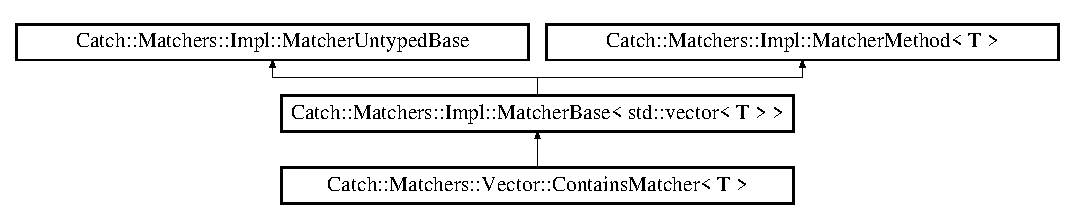
\includegraphics[height=2.514970cm]{struct_catch_1_1_matchers_1_1_vector_1_1_contains_matcher}
\end{center}
\end{figure}
\subsection*{Public Member Functions}
\begin{DoxyCompactItemize}
\item 
\mbox{\Hypertarget{struct_catch_1_1_matchers_1_1_vector_1_1_contains_matcher_ad8e92c8399be6dce75bb5702cdfab700}\label{struct_catch_1_1_matchers_1_1_vector_1_1_contains_matcher_ad8e92c8399be6dce75bb5702cdfab700}} 
{\bfseries Contains\+Matcher} (std\+::vector$<$ T $>$ const \&comparator)
\item 
\mbox{\Hypertarget{struct_catch_1_1_matchers_1_1_vector_1_1_contains_matcher_afd33467ae48a41a634572b41b053f67f}\label{struct_catch_1_1_matchers_1_1_vector_1_1_contains_matcher_afd33467ae48a41a634572b41b053f67f}} 
bool {\bfseries match} (std\+::vector$<$ T $>$ const \&v) const override
\item 
\mbox{\Hypertarget{struct_catch_1_1_matchers_1_1_vector_1_1_contains_matcher_abe6a9ea3d6506c9a1f75ff524f35832e}\label{struct_catch_1_1_matchers_1_1_vector_1_1_contains_matcher_abe6a9ea3d6506c9a1f75ff524f35832e}} 
std\+::string {\bfseries describe} () const override
\end{DoxyCompactItemize}
\subsection*{Public Attributes}
\begin{DoxyCompactItemize}
\item 
\mbox{\Hypertarget{struct_catch_1_1_matchers_1_1_vector_1_1_contains_matcher_a83d051166e4ed0d535219ad6ee99abb2}\label{struct_catch_1_1_matchers_1_1_vector_1_1_contains_matcher_a83d051166e4ed0d535219ad6ee99abb2}} 
std\+::vector$<$ T $>$ const  \& {\bfseries m\+\_\+comparator}
\end{DoxyCompactItemize}
\subsection*{Additional Inherited Members}


The documentation for this struct was generated from the following file\+:\begin{DoxyCompactItemize}
\item 
D\+:/kouluhommat/\+Advanced Object-\/\+Oriented Programming/lopputyö/\+Battleship/\+Battleship/catch.\+hpp\end{DoxyCompactItemize}

\hypertarget{struct_catch_1_1_counts}{}\section{Catch\+:\+:Counts Struct Reference}
\label{struct_catch_1_1_counts}\index{Catch\+::\+Counts@{Catch\+::\+Counts}}
\subsection*{Public Member Functions}
\begin{DoxyCompactItemize}
\item 
\mbox{\Hypertarget{struct_catch_1_1_counts_aaa10666f559057e3e860d2a5a6fae4c4}\label{struct_catch_1_1_counts_aaa10666f559057e3e860d2a5a6fae4c4}} 
\mbox{\hyperlink{struct_catch_1_1_counts}{Counts}} {\bfseries operator-\/} (\mbox{\hyperlink{struct_catch_1_1_counts}{Counts}} const \&other) const
\item 
\mbox{\Hypertarget{struct_catch_1_1_counts_a322a89475cd2cc039140ef371e973677}\label{struct_catch_1_1_counts_a322a89475cd2cc039140ef371e973677}} 
\mbox{\hyperlink{struct_catch_1_1_counts}{Counts}} \& {\bfseries operator+=} (\mbox{\hyperlink{struct_catch_1_1_counts}{Counts}} const \&other)
\item 
\mbox{\Hypertarget{struct_catch_1_1_counts_a94f969c09cf52d1339c085c9603cd1d3}\label{struct_catch_1_1_counts_a94f969c09cf52d1339c085c9603cd1d3}} 
std\+::size\+\_\+t {\bfseries total} () const
\item 
\mbox{\Hypertarget{struct_catch_1_1_counts_a84999490e0ecaa3de5e121bf48eda1b3}\label{struct_catch_1_1_counts_a84999490e0ecaa3de5e121bf48eda1b3}} 
bool {\bfseries all\+Passed} () const
\item 
\mbox{\Hypertarget{struct_catch_1_1_counts_a33bd996e016030155b99fe1c51c08991}\label{struct_catch_1_1_counts_a33bd996e016030155b99fe1c51c08991}} 
bool {\bfseries all\+Ok} () const
\end{DoxyCompactItemize}
\subsection*{Public Attributes}
\begin{DoxyCompactItemize}
\item 
\mbox{\Hypertarget{struct_catch_1_1_counts_ad28daaf3de28006400208b6dd0c631e6}\label{struct_catch_1_1_counts_ad28daaf3de28006400208b6dd0c631e6}} 
std\+::size\+\_\+t {\bfseries passed} = 0
\item 
\mbox{\Hypertarget{struct_catch_1_1_counts_a19982a3817a3bc2c07f0290e71f497a3}\label{struct_catch_1_1_counts_a19982a3817a3bc2c07f0290e71f497a3}} 
std\+::size\+\_\+t {\bfseries failed} = 0
\item 
\mbox{\Hypertarget{struct_catch_1_1_counts_ac090973a2ff51394cd452718e75c073e}\label{struct_catch_1_1_counts_ac090973a2ff51394cd452718e75c073e}} 
std\+::size\+\_\+t {\bfseries failed\+But\+Ok} = 0
\end{DoxyCompactItemize}


The documentation for this struct was generated from the following file\+:\begin{DoxyCompactItemize}
\item 
D\+:/kouluhommat/\+Advanced Object-\/\+Oriented Programming/lopputyö/\+Battleship/\+Battleship/catch.\+hpp\end{DoxyCompactItemize}

\hypertarget{struct_catch_1_1_decomposer}{}\section{Catch\+:\+:Decomposer Struct Reference}
\label{struct_catch_1_1_decomposer}\index{Catch\+::\+Decomposer@{Catch\+::\+Decomposer}}
\subsection*{Public Member Functions}
\begin{DoxyCompactItemize}
\item 
\mbox{\Hypertarget{struct_catch_1_1_decomposer_a20b5b8c0e2ff0328a019ae1a8deca03a}\label{struct_catch_1_1_decomposer_a20b5b8c0e2ff0328a019ae1a8deca03a}} 
{\footnotesize template$<$typename T $>$ }\\auto {\bfseries operator$<$=} (T const \&lhs) -\/$>$ \mbox{\hyperlink{class_catch_1_1_expr_lhs}{Expr\+Lhs}}$<$ T const \&$>$
\item 
\mbox{\Hypertarget{struct_catch_1_1_decomposer_aac129b94903ae1339d5709049d83613b}\label{struct_catch_1_1_decomposer_aac129b94903ae1339d5709049d83613b}} 
auto {\bfseries operator$<$=} (bool value) -\/$>$ \mbox{\hyperlink{class_catch_1_1_expr_lhs}{Expr\+Lhs}}$<$ bool $>$
\end{DoxyCompactItemize}


The documentation for this struct was generated from the following file\+:\begin{DoxyCompactItemize}
\item 
D\+:/kouluhommat/\+Advanced Object-\/\+Oriented Programming/lopputyö/\+Battleship/\+Battleship/catch.\+hpp\end{DoxyCompactItemize}

\hypertarget{class_easy_player}{}\section{Easy\+Player Class Reference}
\label{class_easy_player}\index{Easy\+Player@{Easy\+Player}}


{\ttfamily \#include $<$Easy\+Player.\+h$>$}

Inheritance diagram for Easy\+Player\+:\begin{figure}[H]
\begin{center}
\leavevmode
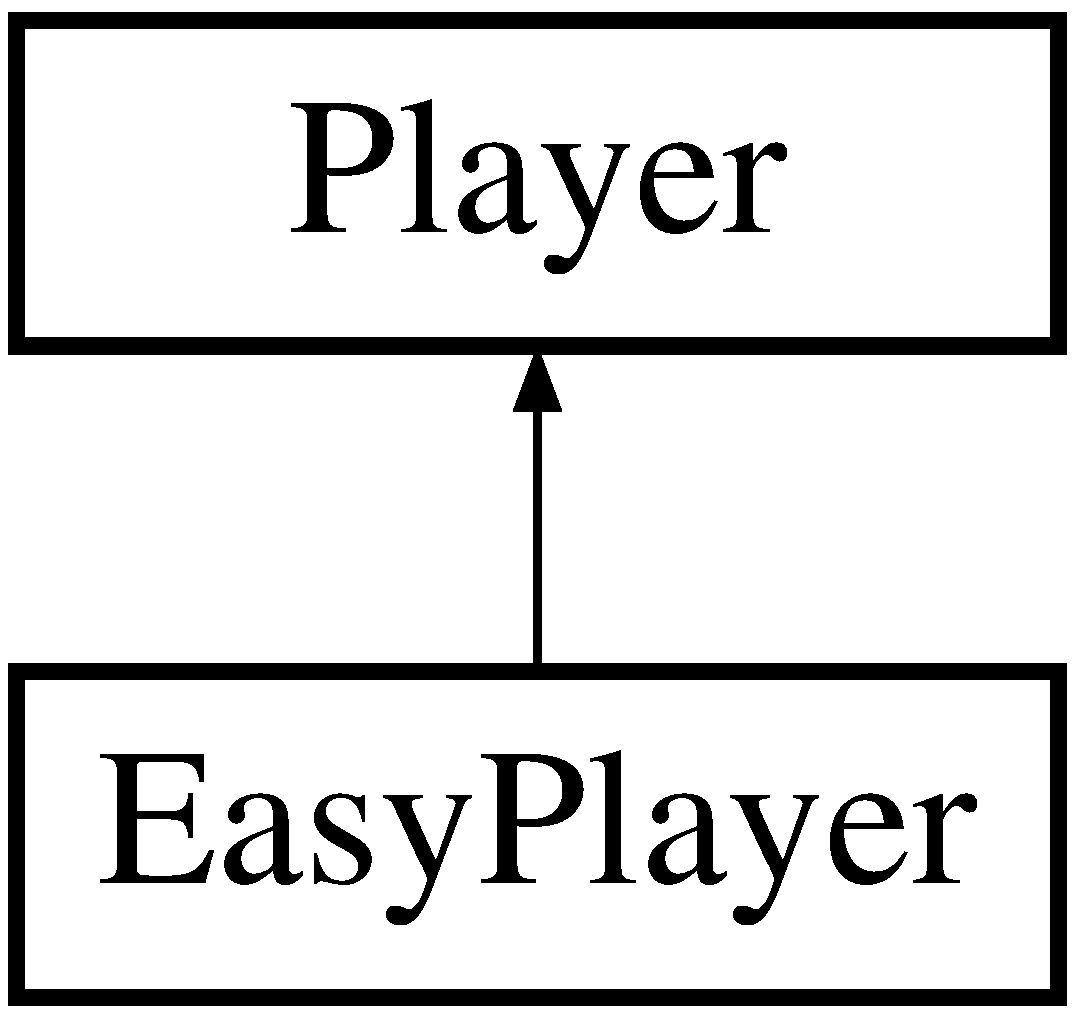
\includegraphics[height=2.000000cm]{class_easy_player}
\end{center}
\end{figure}
\subsection*{Public Member Functions}
\begin{DoxyCompactItemize}
\item 
\mbox{\hyperlink{class_player}{Player}} $\ast$ \mbox{\hyperlink{class_easy_player_a5c9837adc8dd76f5bb9e3ee7a576658f}{create}} (std\+::string nm, const \mbox{\hyperlink{class_game}{Game}} \&g) override
\item 
\mbox{\hyperlink{class_easy_player_abf0692676d0bf3c0eb6f6741c621c7ec}{Easy\+Player}} (std\+::string nm, const \mbox{\hyperlink{class_game}{Game}} \&g)
\begin{DoxyCompactList}\small\item\em Constructor for easy player. \end{DoxyCompactList}\item 
virtual bool \mbox{\hyperlink{class_easy_player_a4b9d5815113f393615412f7a98176a6c}{place\+Ships}} (\mbox{\hyperlink{class_board}{Board}} \&b)
\begin{DoxyCompactList}\small\item\em Method for placing ships. \end{DoxyCompactList}\item 
virtual \mbox{\hyperlink{class_point}{Point}} \mbox{\hyperlink{class_easy_player_a9b00f4a9acc74ff688c609bc15bdbb4d}{recommend}} ()
\begin{DoxyCompactList}\small\item\em Recommends attack for easy player. \end{DoxyCompactList}\item 
virtual void \mbox{\hyperlink{class_easy_player_a254a5ddcd421e1dc71e45125e7ab04d8}{record\+Result}} (\mbox{\hyperlink{class_point}{Point}} p, bool valid\+Shot, bool hit, bool destroyed, int ship\+ID)
\begin{DoxyCompactList}\small\item\em Record attack result. \end{DoxyCompactList}\item 
virtual void \mbox{\hyperlink{class_easy_player_a2121149ace67b4a67a5dfa7633738ea3}{record\+Opponent}} (\mbox{\hyperlink{class_point}{Point}} p)
\begin{DoxyCompactList}\small\item\em Records opponent\textquotesingle{}s result. \end{DoxyCompactList}\end{DoxyCompactItemize}


\subsection{Detailed Description}
\mbox{\hyperlink{class_easy_player}{Easy\+Player}}\+: class declaration of easy bot 

\subsection{Constructor \& Destructor Documentation}
\mbox{\Hypertarget{class_easy_player_abf0692676d0bf3c0eb6f6741c621c7ec}\label{class_easy_player_abf0692676d0bf3c0eb6f6741c621c7ec}} 
\index{Easy\+Player@{Easy\+Player}!Easy\+Player@{Easy\+Player}}
\index{Easy\+Player@{Easy\+Player}!Easy\+Player@{Easy\+Player}}
\subsubsection{\texorpdfstring{Easy\+Player()}{EasyPlayer()}}
{\footnotesize\ttfamily Easy\+Player\+::\+Easy\+Player (\begin{DoxyParamCaption}\item[{std\+::string}]{nm,  }\item[{const \mbox{\hyperlink{class_game}{Game}} \&}]{g }\end{DoxyParamCaption})}



Constructor for easy player. 

Method for creating easy player 
\begin{DoxyParams}{Parameters}
{\em nm} & string containing player name \\
\hline
{\em g} & reference to game object \\
\hline
\end{DoxyParams}


\subsection{Member Function Documentation}
\mbox{\Hypertarget{class_easy_player_a5c9837adc8dd76f5bb9e3ee7a576658f}\label{class_easy_player_a5c9837adc8dd76f5bb9e3ee7a576658f}} 
\index{Easy\+Player@{Easy\+Player}!create@{create}}
\index{create@{create}!Easy\+Player@{Easy\+Player}}
\subsubsection{\texorpdfstring{create()}{create()}}
{\footnotesize\ttfamily \mbox{\hyperlink{class_player}{Player}}$\ast$ Easy\+Player\+::create (\begin{DoxyParamCaption}\item[{std\+::string}]{nm,  }\item[{const \mbox{\hyperlink{class_game}{Game}} \&}]{g }\end{DoxyParamCaption})\hspace{0.3cm}{\ttfamily [inline]}, {\ttfamily [override]}, {\ttfamily [virtual]}}

Pure virtual method for creating a player 
\begin{DoxyParams}{Parameters}
{\em nm} & string containing player\textquotesingle{}s name \\
\hline
{\em g} & reference to game object \\
\hline
\end{DoxyParams}


Implements \mbox{\hyperlink{class_player_a9b9133f3347894da1416953048cecdb2}{Player}}.

\mbox{\Hypertarget{class_easy_player_a4b9d5815113f393615412f7a98176a6c}\label{class_easy_player_a4b9d5815113f393615412f7a98176a6c}} 
\index{Easy\+Player@{Easy\+Player}!place\+Ships@{place\+Ships}}
\index{place\+Ships@{place\+Ships}!Easy\+Player@{Easy\+Player}}
\subsubsection{\texorpdfstring{place\+Ships()}{placeShips()}}
{\footnotesize\ttfamily bool Easy\+Player\+::place\+Ships (\begin{DoxyParamCaption}\item[{\mbox{\hyperlink{class_board}{Board}} \&}]{b }\end{DoxyParamCaption})\hspace{0.3cm}{\ttfamily [virtual]}}



Method for placing ships. 

Method for placing easy player\textquotesingle{}s ships 
\begin{DoxyParams}{Parameters}
{\em b} & Reference to game board object \\
\hline
\end{DoxyParams}
Loops through ships in game

Checks if ship is placed on the game board 

Implements \mbox{\hyperlink{class_player_ab89c1180c7314d3e19bcf4b2bed2e02a}{Player}}.

\mbox{\Hypertarget{class_easy_player_a9b00f4a9acc74ff688c609bc15bdbb4d}\label{class_easy_player_a9b00f4a9acc74ff688c609bc15bdbb4d}} 
\index{Easy\+Player@{Easy\+Player}!recommend@{recommend}}
\index{recommend@{recommend}!Easy\+Player@{Easy\+Player}}
\subsubsection{\texorpdfstring{recommend()}{recommend()}}
{\footnotesize\ttfamily \mbox{\hyperlink{class_point}{Point}} Easy\+Player\+::recommend (\begin{DoxyParamCaption}{ }\end{DoxyParamCaption})\hspace{0.3cm}{\ttfamily [virtual]}}



Recommends attack for easy player. 

Method that recommends attack for easy player Checks if last attacked cell\textquotesingle{}s column is larger than 0

Decreases last attacked cell\textquotesingle{}s column with game\textquotesingle{}s columns -\/ 1

Checks if last attacked cell\textquotesingle{}s rows is larger than 0

Decreases last attacked cell\textquotesingle{}s rows with game\textquotesingle{}s rows -\/ 1 

Implements \mbox{\hyperlink{class_player_a2cc7a83d11158eafd8d49d4b9f23ce56}{Player}}.

\mbox{\Hypertarget{class_easy_player_a2121149ace67b4a67a5dfa7633738ea3}\label{class_easy_player_a2121149ace67b4a67a5dfa7633738ea3}} 
\index{Easy\+Player@{Easy\+Player}!record\+Opponent@{record\+Opponent}}
\index{record\+Opponent@{record\+Opponent}!Easy\+Player@{Easy\+Player}}
\subsubsection{\texorpdfstring{record\+Opponent()}{recordOpponent()}}
{\footnotesize\ttfamily void Easy\+Player\+::record\+Opponent (\begin{DoxyParamCaption}\item[{\mbox{\hyperlink{class_point}{Point}}}]{p }\end{DoxyParamCaption})\hspace{0.3cm}{\ttfamily [virtual]}}



Records opponent\textquotesingle{}s result. 

Method for recording opponent\textquotesingle{}s result 
\begin{DoxyParams}{Parameters}
{\em p} & \mbox{\hyperlink{class_point}{Point}} containing attacked cell \\
\hline
\end{DoxyParams}


Implements \mbox{\hyperlink{class_player_a768e14edee61e208e6fd295cdd72a49c}{Player}}.

\mbox{\Hypertarget{class_easy_player_a254a5ddcd421e1dc71e45125e7ab04d8}\label{class_easy_player_a254a5ddcd421e1dc71e45125e7ab04d8}} 
\index{Easy\+Player@{Easy\+Player}!record\+Result@{record\+Result}}
\index{record\+Result@{record\+Result}!Easy\+Player@{Easy\+Player}}
\subsubsection{\texorpdfstring{record\+Result()}{recordResult()}}
{\footnotesize\ttfamily void Easy\+Player\+::record\+Result (\begin{DoxyParamCaption}\item[{\mbox{\hyperlink{class_point}{Point}}}]{p,  }\item[{bool}]{valid\+Shot,  }\item[{bool}]{hit,  }\item[{bool}]{destroyed,  }\item[{int}]{ship\+ID }\end{DoxyParamCaption})\hspace{0.3cm}{\ttfamily [virtual]}}



Record attack result. 

Method for recording result 
\begin{DoxyParams}{Parameters}
{\em p} & \mbox{\hyperlink{class_point}{Point}} containing attacked cell \\
\hline
{\em valid\+Shot} & boolean that checks if attack was valid \\
\hline
{\em hit} & boolean to check if ship was hit @ \\
\hline
\end{DoxyParams}


Implements \mbox{\hyperlink{class_player_a368527cfefaac58dc942b32658f977ed}{Player}}.



The documentation for this class was generated from the following files\+:\begin{DoxyCompactItemize}
\item 
D\+:/kouluhommat/\+Advanced Object-\/\+Oriented Programming/lopputyö/\+Battleship/\+Battleship/\mbox{\hyperlink{_easy_player_8h}{Easy\+Player.\+h}}\item 
D\+:/kouluhommat/\+Advanced Object-\/\+Oriented Programming/lopputyö/\+Battleship/\+Battleship/\mbox{\hyperlink{_player_8cpp}{Player.\+cpp}}\end{DoxyCompactItemize}

\hypertarget{struct_catch_1_1_matchers_1_1_std_string_1_1_ends_with_matcher}{}\section{Catch\+:\+:Matchers\+:\+:Std\+String\+:\+:Ends\+With\+Matcher Struct Reference}
\label{struct_catch_1_1_matchers_1_1_std_string_1_1_ends_with_matcher}\index{Catch\+::\+Matchers\+::\+Std\+String\+::\+Ends\+With\+Matcher@{Catch\+::\+Matchers\+::\+Std\+String\+::\+Ends\+With\+Matcher}}
Inheritance diagram for Catch\+:\+:Matchers\+:\+:Std\+String\+:\+:Ends\+With\+Matcher\+:\begin{figure}[H]
\begin{center}
\leavevmode
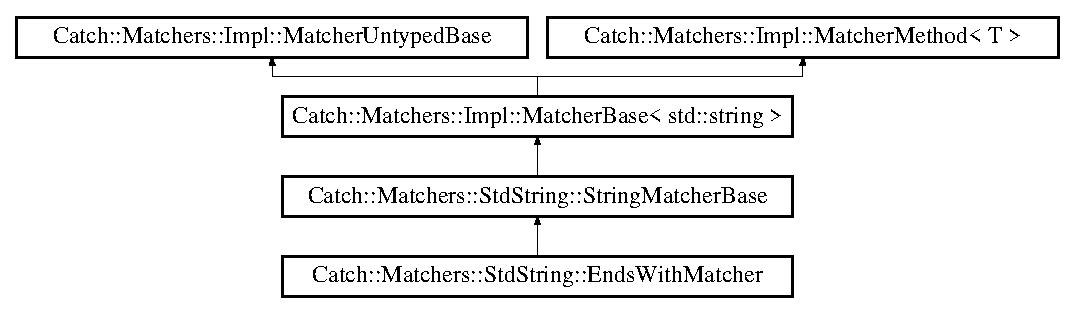
\includegraphics[height=3.758389cm]{struct_catch_1_1_matchers_1_1_std_string_1_1_ends_with_matcher}
\end{center}
\end{figure}
\subsection*{Public Member Functions}
\begin{DoxyCompactItemize}
\item 
\mbox{\Hypertarget{struct_catch_1_1_matchers_1_1_std_string_1_1_ends_with_matcher_aa5ec700b4629562f74f362080accfd7b}\label{struct_catch_1_1_matchers_1_1_std_string_1_1_ends_with_matcher_aa5ec700b4629562f74f362080accfd7b}} 
{\bfseries Ends\+With\+Matcher} (\mbox{\hyperlink{struct_catch_1_1_matchers_1_1_std_string_1_1_cased_string}{Cased\+String}} const \&comparator)
\item 
\mbox{\Hypertarget{struct_catch_1_1_matchers_1_1_std_string_1_1_ends_with_matcher_aca2741fa57374a2a98d2a84ac3e13a6d}\label{struct_catch_1_1_matchers_1_1_std_string_1_1_ends_with_matcher_aca2741fa57374a2a98d2a84ac3e13a6d}} 
bool {\bfseries match} (std\+::string const \&source) const override
\end{DoxyCompactItemize}
\subsection*{Additional Inherited Members}


The documentation for this struct was generated from the following file\+:\begin{DoxyCompactItemize}
\item 
D\+:/kouluhommat/\+Advanced Object-\/\+Oriented Programming/lopputyö/\+Battleship/\+Battleship/catch.\+hpp\end{DoxyCompactItemize}

\hypertarget{struct_catch_1_1_matchers_1_1_std_string_1_1_equals_matcher}{}\section{Catch\+:\+:Matchers\+:\+:Std\+String\+:\+:Equals\+Matcher Struct Reference}
\label{struct_catch_1_1_matchers_1_1_std_string_1_1_equals_matcher}\index{Catch\+::\+Matchers\+::\+Std\+String\+::\+Equals\+Matcher@{Catch\+::\+Matchers\+::\+Std\+String\+::\+Equals\+Matcher}}
Inheritance diagram for Catch\+:\+:Matchers\+:\+:Std\+String\+:\+:Equals\+Matcher\+:\begin{figure}[H]
\begin{center}
\leavevmode
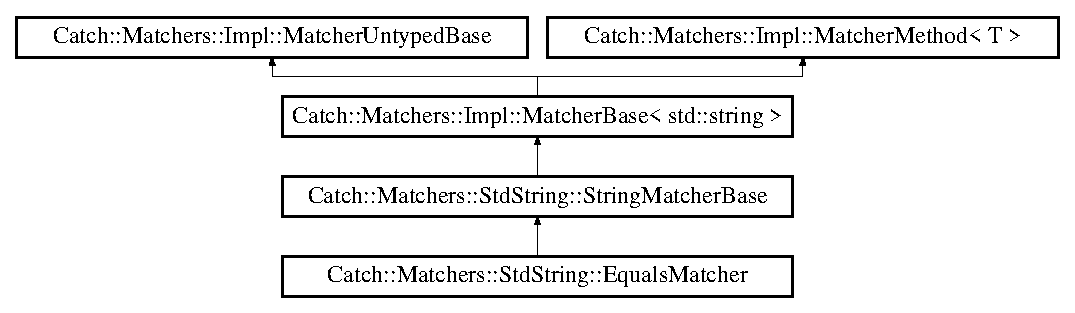
\includegraphics[height=3.758389cm]{struct_catch_1_1_matchers_1_1_std_string_1_1_equals_matcher}
\end{center}
\end{figure}
\subsection*{Public Member Functions}
\begin{DoxyCompactItemize}
\item 
\mbox{\Hypertarget{struct_catch_1_1_matchers_1_1_std_string_1_1_equals_matcher_ab740f1fb2310e9fe3fed5134d4c7e4c8}\label{struct_catch_1_1_matchers_1_1_std_string_1_1_equals_matcher_ab740f1fb2310e9fe3fed5134d4c7e4c8}} 
{\bfseries Equals\+Matcher} (\mbox{\hyperlink{struct_catch_1_1_matchers_1_1_std_string_1_1_cased_string}{Cased\+String}} const \&comparator)
\item 
\mbox{\Hypertarget{struct_catch_1_1_matchers_1_1_std_string_1_1_equals_matcher_a0bb9d64693f7bb1ef7441062d219f21a}\label{struct_catch_1_1_matchers_1_1_std_string_1_1_equals_matcher_a0bb9d64693f7bb1ef7441062d219f21a}} 
bool {\bfseries match} (std\+::string const \&source) const override
\end{DoxyCompactItemize}
\subsection*{Additional Inherited Members}


The documentation for this struct was generated from the following file\+:\begin{DoxyCompactItemize}
\item 
D\+:/kouluhommat/\+Advanced Object-\/\+Oriented Programming/lopputyö/\+Battleship/\+Battleship/catch.\+hpp\end{DoxyCompactItemize}

\hypertarget{struct_catch_1_1_matchers_1_1_vector_1_1_equals_matcher}{}\section{Catch\+:\+:Matchers\+:\+:Vector\+:\+:Equals\+Matcher$<$ T $>$ Struct Template Reference}
\label{struct_catch_1_1_matchers_1_1_vector_1_1_equals_matcher}\index{Catch\+::\+Matchers\+::\+Vector\+::\+Equals\+Matcher$<$ T $>$@{Catch\+::\+Matchers\+::\+Vector\+::\+Equals\+Matcher$<$ T $>$}}
Inheritance diagram for Catch\+:\+:Matchers\+:\+:Vector\+:\+:Equals\+Matcher$<$ T $>$\+:\begin{figure}[H]
\begin{center}
\leavevmode
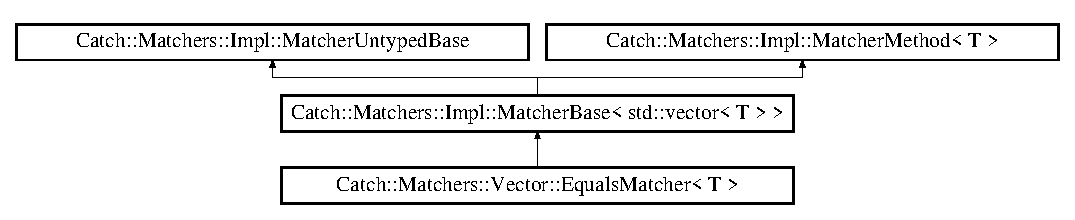
\includegraphics[height=2.514970cm]{struct_catch_1_1_matchers_1_1_vector_1_1_equals_matcher}
\end{center}
\end{figure}
\subsection*{Public Member Functions}
\begin{DoxyCompactItemize}
\item 
\mbox{\Hypertarget{struct_catch_1_1_matchers_1_1_vector_1_1_equals_matcher_a3846c47780d1991dcfe87aefded98008}\label{struct_catch_1_1_matchers_1_1_vector_1_1_equals_matcher_a3846c47780d1991dcfe87aefded98008}} 
{\bfseries Equals\+Matcher} (std\+::vector$<$ T $>$ const \&comparator)
\item 
\mbox{\Hypertarget{struct_catch_1_1_matchers_1_1_vector_1_1_equals_matcher_a2d96cca58a44151fddc5257eda3305da}\label{struct_catch_1_1_matchers_1_1_vector_1_1_equals_matcher_a2d96cca58a44151fddc5257eda3305da}} 
bool {\bfseries match} (std\+::vector$<$ T $>$ const \&v) const override
\item 
\mbox{\Hypertarget{struct_catch_1_1_matchers_1_1_vector_1_1_equals_matcher_a36b5f7ecada4081d6c65bebe8ddea6f4}\label{struct_catch_1_1_matchers_1_1_vector_1_1_equals_matcher_a36b5f7ecada4081d6c65bebe8ddea6f4}} 
std\+::string {\bfseries describe} () const override
\end{DoxyCompactItemize}
\subsection*{Public Attributes}
\begin{DoxyCompactItemize}
\item 
\mbox{\Hypertarget{struct_catch_1_1_matchers_1_1_vector_1_1_equals_matcher_a56f7aa6f110a12b1b9aeb0cabbc9d755}\label{struct_catch_1_1_matchers_1_1_vector_1_1_equals_matcher_a56f7aa6f110a12b1b9aeb0cabbc9d755}} 
std\+::vector$<$ T $>$ const  \& {\bfseries m\+\_\+comparator}
\end{DoxyCompactItemize}
\subsection*{Additional Inherited Members}


The documentation for this struct was generated from the following file\+:\begin{DoxyCompactItemize}
\item 
D\+:/kouluhommat/\+Advanced Object-\/\+Oriented Programming/lopputyö/\+Battleship/\+Battleship/catch.\+hpp\end{DoxyCompactItemize}

\hypertarget{class_catch_1_1_exception_translator_registrar}{}\section{Catch\+:\+:Exception\+Translator\+Registrar Class Reference}
\label{class_catch_1_1_exception_translator_registrar}\index{Catch\+::\+Exception\+Translator\+Registrar@{Catch\+::\+Exception\+Translator\+Registrar}}
\subsection*{Public Member Functions}
\begin{DoxyCompactItemize}
\item 
\mbox{\Hypertarget{class_catch_1_1_exception_translator_registrar_aa73229de911f26b1df6c6c87c4d9e04e}\label{class_catch_1_1_exception_translator_registrar_aa73229de911f26b1df6c6c87c4d9e04e}} 
{\footnotesize template$<$typename T $>$ }\\{\bfseries Exception\+Translator\+Registrar} (std\+::string($\ast$translate\+Function)(T \&))
\end{DoxyCompactItemize}


The documentation for this class was generated from the following file\+:\begin{DoxyCompactItemize}
\item 
D\+:/kouluhommat/\+Advanced Object-\/\+Oriented Programming/lopputyö/\+Battleship/\+Battleship/catch.\+hpp\end{DoxyCompactItemize}

\hypertarget{class_catch_1_1_expr_lhs}{}\section{Catch\+:\+:Expr\+Lhs$<$ LhsT $>$ Class Template Reference}
\label{class_catch_1_1_expr_lhs}\index{Catch\+::\+Expr\+Lhs$<$ Lhs\+T $>$@{Catch\+::\+Expr\+Lhs$<$ Lhs\+T $>$}}
\subsection*{Public Member Functions}
\begin{DoxyCompactItemize}
\item 
\mbox{\Hypertarget{class_catch_1_1_expr_lhs_ad22c6af1a7d6993240624d299714a479}\label{class_catch_1_1_expr_lhs_ad22c6af1a7d6993240624d299714a479}} 
{\bfseries Expr\+Lhs} (LhsT lhs)
\item 
\mbox{\Hypertarget{class_catch_1_1_expr_lhs_a3068adff1dbbaeec62ffc368d4d6cc4d}\label{class_catch_1_1_expr_lhs_a3068adff1dbbaeec62ffc368d4d6cc4d}} 
{\footnotesize template$<$typename RhsT $>$ }\\auto {\bfseries operator==} (RhsT const \&rhs) -\/$>$ \mbox{\hyperlink{class_catch_1_1_binary_expr}{Binary\+Expr}}$<$ LhsT, RhsT const \&$>$ const
\item 
\mbox{\Hypertarget{class_catch_1_1_expr_lhs_ab707a84abdffbdc35962a495e238d393}\label{class_catch_1_1_expr_lhs_ab707a84abdffbdc35962a495e238d393}} 
auto {\bfseries operator==} (bool rhs) -\/$>$ \mbox{\hyperlink{class_catch_1_1_binary_expr}{Binary\+Expr}}$<$ LhsT, bool $>$ const
\item 
\mbox{\Hypertarget{class_catch_1_1_expr_lhs_a5e10eab8aed53dd000b89d8fd7754437}\label{class_catch_1_1_expr_lhs_a5e10eab8aed53dd000b89d8fd7754437}} 
{\footnotesize template$<$typename RhsT $>$ }\\auto {\bfseries operator!=} (RhsT const \&rhs) -\/$>$ \mbox{\hyperlink{class_catch_1_1_binary_expr}{Binary\+Expr}}$<$ LhsT, RhsT const \&$>$ const
\item 
\mbox{\Hypertarget{class_catch_1_1_expr_lhs_a60eca847201d057d8a8b7222c69b619c}\label{class_catch_1_1_expr_lhs_a60eca847201d057d8a8b7222c69b619c}} 
auto {\bfseries operator!=} (bool rhs) -\/$>$ \mbox{\hyperlink{class_catch_1_1_binary_expr}{Binary\+Expr}}$<$ LhsT, bool $>$ const
\item 
\mbox{\Hypertarget{class_catch_1_1_expr_lhs_a23cb0cd983a1ac9c3df5160542199b83}\label{class_catch_1_1_expr_lhs_a23cb0cd983a1ac9c3df5160542199b83}} 
{\footnotesize template$<$typename RhsT $>$ }\\auto {\bfseries operator$>$} (RhsT const \&rhs) -\/$>$ \mbox{\hyperlink{class_catch_1_1_binary_expr}{Binary\+Expr}}$<$ LhsT, RhsT const \&$>$ const
\item 
\mbox{\Hypertarget{class_catch_1_1_expr_lhs_a55284221df2edb3542e765c87b5691b9}\label{class_catch_1_1_expr_lhs_a55284221df2edb3542e765c87b5691b9}} 
{\footnotesize template$<$typename RhsT $>$ }\\auto {\bfseries operator$<$} (RhsT const \&rhs) -\/$>$ \mbox{\hyperlink{class_catch_1_1_binary_expr}{Binary\+Expr}}$<$ LhsT, RhsT const \&$>$ const
\item 
\mbox{\Hypertarget{class_catch_1_1_expr_lhs_aff594ae5b957105c517a6257d2e730f0}\label{class_catch_1_1_expr_lhs_aff594ae5b957105c517a6257d2e730f0}} 
{\footnotesize template$<$typename RhsT $>$ }\\auto {\bfseries operator$>$=} (RhsT const \&rhs) -\/$>$ \mbox{\hyperlink{class_catch_1_1_binary_expr}{Binary\+Expr}}$<$ LhsT, RhsT const \&$>$ const
\item 
\mbox{\Hypertarget{class_catch_1_1_expr_lhs_a6bd8a22c1a7fe2f66d71d7196f20af4f}\label{class_catch_1_1_expr_lhs_a6bd8a22c1a7fe2f66d71d7196f20af4f}} 
{\footnotesize template$<$typename RhsT $>$ }\\auto {\bfseries operator$<$=} (RhsT const \&rhs) -\/$>$ \mbox{\hyperlink{class_catch_1_1_binary_expr}{Binary\+Expr}}$<$ LhsT, RhsT const \&$>$ const
\item 
\mbox{\Hypertarget{class_catch_1_1_expr_lhs_ab68bd6d5d3ae21b7fba9010150fba95d}\label{class_catch_1_1_expr_lhs_ab68bd6d5d3ae21b7fba9010150fba95d}} 
auto {\bfseries make\+Unary\+Expr} () const -\/$>$ \mbox{\hyperlink{class_catch_1_1_unary_expr}{Unary\+Expr}}$<$ LhsT $>$
\end{DoxyCompactItemize}


The documentation for this class was generated from the following file\+:\begin{DoxyCompactItemize}
\item 
D\+:/kouluhommat/\+Advanced Object-\/\+Oriented Programming/lopputyö/\+Battleship/\+Battleship/catch.\+hpp\end{DoxyCompactItemize}

\hypertarget{class_catch_1_1_generators_1_1_fixed_values_generator}{}\section{Catch\+:\+:Generators\+:\+:Fixed\+Values\+Generator$<$ T $>$ Class Template Reference}
\label{class_catch_1_1_generators_1_1_fixed_values_generator}\index{Catch\+::\+Generators\+::\+Fixed\+Values\+Generator$<$ T $>$@{Catch\+::\+Generators\+::\+Fixed\+Values\+Generator$<$ T $>$}}
Inheritance diagram for Catch\+:\+:Generators\+:\+:Fixed\+Values\+Generator$<$ T $>$\+:\begin{figure}[H]
\begin{center}
\leavevmode
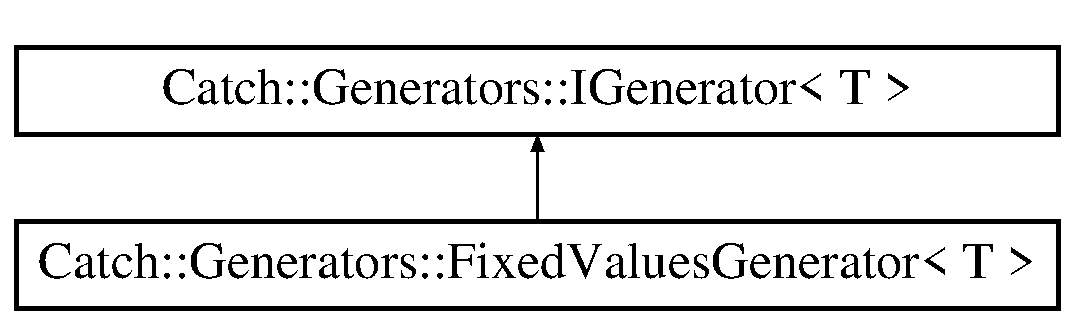
\includegraphics[height=2.000000cm]{class_catch_1_1_generators_1_1_fixed_values_generator}
\end{center}
\end{figure}
\subsection*{Public Member Functions}
\begin{DoxyCompactItemize}
\item 
\mbox{\Hypertarget{class_catch_1_1_generators_1_1_fixed_values_generator_a6e9f473655413c1cb15f079890f06b86}\label{class_catch_1_1_generators_1_1_fixed_values_generator_a6e9f473655413c1cb15f079890f06b86}} 
{\bfseries Fixed\+Values\+Generator} (std\+::initializer\+\_\+list$<$ T $>$ values)
\item 
\mbox{\Hypertarget{class_catch_1_1_generators_1_1_fixed_values_generator_a3ed654a5860c170dbe7b01487b83253d}\label{class_catch_1_1_generators_1_1_fixed_values_generator_a3ed654a5860c170dbe7b01487b83253d}} 
auto {\bfseries get} (size\+\_\+t index) const -\/$>$ T override
\end{DoxyCompactItemize}


The documentation for this class was generated from the following file\+:\begin{DoxyCompactItemize}
\item 
D\+:/kouluhommat/\+Advanced Object-\/\+Oriented Programming/lopputyö/\+Battleship/\+Battleship/catch.\+hpp\end{DoxyCompactItemize}

\hypertarget{class_game}{}\section{Game Class Reference}
\label{class_game}\index{Game@{Game}}


Declaration for game implementation class.  




{\ttfamily \#include $<$Game.\+h$>$}

\subsection*{Public Member Functions}
\begin{DoxyCompactItemize}
\item 
\mbox{\hyperlink{class_game_a848102f31ba288bac7aa39db4378db7a}{Game}} (int n\+Rows, int n\+Cols)
\begin{DoxyCompactList}\small\item\em Constructor for game object. \end{DoxyCompactList}\item 
\mbox{\hyperlink{class_game_ae3d112ca6e0e55150d2fdbc704474530}{$\sim$\+Game}} ()
\begin{DoxyCompactList}\small\item\em Destructor for game object. \end{DoxyCompactList}\item 
int \mbox{\hyperlink{class_game_a0a0531ce88923b4fbe2b3fea4c9d27f5}{rows}} () const
\begin{DoxyCompactList}\small\item\em Getter for game\textquotesingle{}s rows. \end{DoxyCompactList}\item 
int \mbox{\hyperlink{class_game_afbb769ac9dc75bd26e33a74a3cce5009}{cols}} () const
\begin{DoxyCompactList}\small\item\em Getter for game\textquotesingle{}s columns. \end{DoxyCompactList}\item 
int \mbox{\hyperlink{class_game_a783885809649e4799b199ece36c72be0}{n\+Ships}} () const
\begin{DoxyCompactList}\small\item\em Getter for number of ships. \end{DoxyCompactList}\item 
int \mbox{\hyperlink{class_game_af447d664cda0ae50f98afaa1e75ec0e3}{ship\+Length}} (int ship\+ID) const
\begin{DoxyCompactList}\small\item\em Getter for ship\textquotesingle{}s length. \end{DoxyCompactList}\item 
char \mbox{\hyperlink{class_game_a4d7e709c85b6abd5defa24f5f78cd1d1}{ship\+Symbol}} (int ship\+ID) const
\begin{DoxyCompactList}\small\item\em Getter for ship\textquotesingle{}s symbol. \end{DoxyCompactList}\item 
std\+::string \mbox{\hyperlink{class_game_aa652b00557acd25657c4aeface33d29a}{ship\+Name}} (int ship\+ID) const
\begin{DoxyCompactList}\small\item\em Getter for ship\textquotesingle{}s name. \end{DoxyCompactList}\item 
bool \mbox{\hyperlink{class_game_a3ec9ae2ce5d1ac1cbf4ed18aa7141744}{valid}} (\mbox{\hyperlink{class_point}{Point}} p) const
\begin{DoxyCompactList}\small\item\em Checks if shot is valid. \end{DoxyCompactList}\item 
bool \mbox{\hyperlink{class_game_a3ac4fd5a820cafec68f05cc81c26492a}{add\+Ship}} (int length, char symbol, std\+::string name)
\begin{DoxyCompactList}\small\item\em Adds ship into game. \end{DoxyCompactList}\item 
\mbox{\hyperlink{class_point}{Point}} \mbox{\hyperlink{class_game_acd99c992d69fe990abfb16ab1bde177c}{rnd\+Point}} () const
\begin{DoxyCompactList}\small\item\em Getter for random point. \end{DoxyCompactList}\item 
\mbox{\hyperlink{class_player}{Player}} $\ast$ \mbox{\hyperlink{class_game_a9102360e66754f58044c93d80260f6d0}{play}} (\mbox{\hyperlink{class_player}{Player}} $\ast$p1, \mbox{\hyperlink{class_player}{Player}} $\ast$p2, bool pause=true)
\item 
\mbox{\Hypertarget{class_game_abb28875d74d25fa9e0dcdbe37c6ad89c}\label{class_game_abb28875d74d25fa9e0dcdbe37c6ad89c}} 
\mbox{\hyperlink{class_game_abb28875d74d25fa9e0dcdbe37c6ad89c}{Game}} (const \mbox{\hyperlink{class_game}{Game}} \&)=delete
\begin{DoxyCompactList}\small\item\em Prevents game object from being copied/assigned. \end{DoxyCompactList}\item 
\mbox{\Hypertarget{class_game_a4d0c0503733cc50b0b5cb8d7ef1237ec}\label{class_game_a4d0c0503733cc50b0b5cb8d7ef1237ec}} 
\mbox{\hyperlink{class_game}{Game}} \& {\bfseries operator=} (const \mbox{\hyperlink{class_game}{Game}} \&)=delete
\end{DoxyCompactItemize}


\subsection{Detailed Description}
Declaration for game implementation class. 

\subsection{Constructor \& Destructor Documentation}
\mbox{\Hypertarget{class_game_a848102f31ba288bac7aa39db4378db7a}\label{class_game_a848102f31ba288bac7aa39db4378db7a}} 
\index{Game@{Game}!Game@{Game}}
\index{Game@{Game}!Game@{Game}}
\subsubsection{\texorpdfstring{Game()}{Game()}}
{\footnotesize\ttfamily Game\+::\+Game (\begin{DoxyParamCaption}\item[{int}]{n\+Rows,  }\item[{int}]{n\+Cols }\end{DoxyParamCaption})}



Constructor for game object. 

Delegates to game implementation 
\begin{DoxyParams}{Parameters}
{\em n\+Rows} & integer containing number of rows \\
\hline
{\em n\+Cols} & integer containing number of columns \\
\hline
\end{DoxyParams}
Checks if the number of rows is valid \mbox{\Hypertarget{class_game_ae3d112ca6e0e55150d2fdbc704474530}\label{class_game_ae3d112ca6e0e55150d2fdbc704474530}} 
\index{Game@{Game}!````~Game@{$\sim$\+Game}}
\index{````~Game@{$\sim$\+Game}!Game@{Game}}
\subsubsection{\texorpdfstring{$\sim$\+Game()}{~Game()}}
{\footnotesize\ttfamily Game\+::$\sim$\+Game (\begin{DoxyParamCaption}{ }\end{DoxyParamCaption})}



Destructor for game object. 

Deletes to game implementation 

\subsection{Member Function Documentation}
\mbox{\Hypertarget{class_game_a3ac4fd5a820cafec68f05cc81c26492a}\label{class_game_a3ac4fd5a820cafec68f05cc81c26492a}} 
\index{Game@{Game}!add\+Ship@{add\+Ship}}
\index{add\+Ship@{add\+Ship}!Game@{Game}}
\subsubsection{\texorpdfstring{add\+Ship()}{addShip()}}
{\footnotesize\ttfamily bool Game\+::add\+Ship (\begin{DoxyParamCaption}\item[{int}]{length,  }\item[{char}]{symbol,  }\item[{std\+::string}]{name }\end{DoxyParamCaption})}



Adds ship into game. 

Delegates to game implementations add\+Ships method Checks if the ship\textquotesingle{}s parameters are valid 
\begin{DoxyParams}{Parameters}
{\em length} & integer containing ship\textquotesingle{}s length \\
\hline
{\em symbol} & character containing ship\textquotesingle{}s symbol \\
\hline
{\em name} & string containing ship\textquotesingle{}s name \\
\hline
\end{DoxyParams}
Checks if ship\textquotesingle{}s length is less than 1

Checks if ship fits into the board

Checks if ship\textquotesingle{}s character is valid

Checks if ship\textquotesingle{}s symbol is already in use for other reasons

$<$ Total length of the ships ~\newline
~\newline
~\newline
 Loops through ships and adds into total length

Checks if ship symbol is already used by another ship

Checks if the game board is too small for all the ships \mbox{\Hypertarget{class_game_afbb769ac9dc75bd26e33a74a3cce5009}\label{class_game_afbb769ac9dc75bd26e33a74a3cce5009}} 
\index{Game@{Game}!cols@{cols}}
\index{cols@{cols}!Game@{Game}}
\subsubsection{\texorpdfstring{cols()}{cols()}}
{\footnotesize\ttfamily int Game\+::cols (\begin{DoxyParamCaption}{ }\end{DoxyParamCaption}) const}



Getter for game\textquotesingle{}s columns. 

Delegates to game implementations columns method \mbox{\Hypertarget{class_game_a783885809649e4799b199ece36c72be0}\label{class_game_a783885809649e4799b199ece36c72be0}} 
\index{Game@{Game}!n\+Ships@{n\+Ships}}
\index{n\+Ships@{n\+Ships}!Game@{Game}}
\subsubsection{\texorpdfstring{n\+Ships()}{nShips()}}
{\footnotesize\ttfamily int Game\+::n\+Ships (\begin{DoxyParamCaption}{ }\end{DoxyParamCaption}) const}



Getter for number of ships. 

Delegates into game implementations number of ships method \mbox{\Hypertarget{class_game_a9102360e66754f58044c93d80260f6d0}\label{class_game_a9102360e66754f58044c93d80260f6d0}} 
\index{Game@{Game}!play@{play}}
\index{play@{play}!Game@{Game}}
\subsubsection{\texorpdfstring{play()}{play()}}
{\footnotesize\ttfamily \mbox{\hyperlink{class_player}{Player}} $\ast$ Game\+::play (\begin{DoxyParamCaption}\item[{\mbox{\hyperlink{class_player}{Player}} $\ast$}]{p1,  }\item[{\mbox{\hyperlink{class_player}{Player}} $\ast$}]{p2,  }\item[{bool}]{pause = {\ttfamily true} }\end{DoxyParamCaption})}

Method for playing game

Delegates to game implementations play method 
\begin{DoxyParams}{Parameters}
{\em p1} & pointer for first player \\
\hline
{\em p2} & pointer for second player \\
\hline
{\em pause} & boolean for pausing game \\
\hline
\end{DoxyParams}
Checks if players are null pointers and there are no ships

Uses copy of this object to create boards \mbox{\Hypertarget{class_game_acd99c992d69fe990abfb16ab1bde177c}\label{class_game_acd99c992d69fe990abfb16ab1bde177c}} 
\index{Game@{Game}!rnd\+Point@{rnd\+Point}}
\index{rnd\+Point@{rnd\+Point}!Game@{Game}}
\subsubsection{\texorpdfstring{rnd\+Point()}{rndPoint()}}
{\footnotesize\ttfamily \mbox{\hyperlink{class_point}{Point}} Game\+::rnd\+Point (\begin{DoxyParamCaption}{ }\end{DoxyParamCaption}) const}



Getter for random point. 

Delegates into game implementation\textquotesingle{}s random point method \mbox{\Hypertarget{class_game_a0a0531ce88923b4fbe2b3fea4c9d27f5}\label{class_game_a0a0531ce88923b4fbe2b3fea4c9d27f5}} 
\index{Game@{Game}!rows@{rows}}
\index{rows@{rows}!Game@{Game}}
\subsubsection{\texorpdfstring{rows()}{rows()}}
{\footnotesize\ttfamily int Game\+::rows (\begin{DoxyParamCaption}{ }\end{DoxyParamCaption}) const}



Getter for game\textquotesingle{}s rows. 

Delegates to game implementations rows method \mbox{\Hypertarget{class_game_af447d664cda0ae50f98afaa1e75ec0e3}\label{class_game_af447d664cda0ae50f98afaa1e75ec0e3}} 
\index{Game@{Game}!ship\+Length@{ship\+Length}}
\index{ship\+Length@{ship\+Length}!Game@{Game}}
\subsubsection{\texorpdfstring{ship\+Length()}{shipLength()}}
{\footnotesize\ttfamily int Game\+::ship\+Length (\begin{DoxyParamCaption}\item[{int}]{ship\+ID }\end{DoxyParamCaption}) const}



Getter for ship\textquotesingle{}s length. 

Delegates to game implementations ship length method Asserts that ship\+ID is more than 0 and less than number of ships 
\begin{DoxyParams}{Parameters}
{\em ship\+ID} & integer containing ship\textquotesingle{}s id \\
\hline
\end{DoxyParams}
\mbox{\Hypertarget{class_game_aa652b00557acd25657c4aeface33d29a}\label{class_game_aa652b00557acd25657c4aeface33d29a}} 
\index{Game@{Game}!ship\+Name@{ship\+Name}}
\index{ship\+Name@{ship\+Name}!Game@{Game}}
\subsubsection{\texorpdfstring{ship\+Name()}{shipName()}}
{\footnotesize\ttfamily string Game\+::ship\+Name (\begin{DoxyParamCaption}\item[{int}]{ship\+ID }\end{DoxyParamCaption}) const}



Getter for ship\textquotesingle{}s name. 

Delegates to game implementations ship name method Asserts that ship\+ID is more than 0 and less than number of ships 
\begin{DoxyParams}{Parameters}
{\em ship\+ID} & integer containing ship\textquotesingle{}s id \\
\hline
\end{DoxyParams}
\mbox{\Hypertarget{class_game_a4d7e709c85b6abd5defa24f5f78cd1d1}\label{class_game_a4d7e709c85b6abd5defa24f5f78cd1d1}} 
\index{Game@{Game}!ship\+Symbol@{ship\+Symbol}}
\index{ship\+Symbol@{ship\+Symbol}!Game@{Game}}
\subsubsection{\texorpdfstring{ship\+Symbol()}{shipSymbol()}}
{\footnotesize\ttfamily char Game\+::ship\+Symbol (\begin{DoxyParamCaption}\item[{int}]{ship\+ID }\end{DoxyParamCaption}) const}



Getter for ship\textquotesingle{}s symbol. 

Delegates to game implementations ship symbol method Asserts that ship\+ID is more than 0 and less than number of ships 
\begin{DoxyParams}{Parameters}
{\em ship\+ID} & integer containing ship\textquotesingle{}s id \\
\hline
\end{DoxyParams}
\mbox{\Hypertarget{class_game_a3ec9ae2ce5d1ac1cbf4ed18aa7141744}\label{class_game_a3ec9ae2ce5d1ac1cbf4ed18aa7141744}} 
\index{Game@{Game}!valid@{valid}}
\index{valid@{valid}!Game@{Game}}
\subsubsection{\texorpdfstring{valid()}{valid()}}
{\footnotesize\ttfamily bool Game\+::valid (\begin{DoxyParamCaption}\item[{\mbox{\hyperlink{class_point}{Point}}}]{p }\end{DoxyParamCaption}) const}



Checks if shot is valid. 

Delegates to game implementations valid method 

The documentation for this class was generated from the following files\+:\begin{DoxyCompactItemize}
\item 
D\+:/kouluhommat/\+Advanced Object-\/\+Oriented Programming/lopputyö/\+Battleship/\+Battleship/\mbox{\hyperlink{_game_8h}{Game.\+h}}\item 
D\+:/kouluhommat/\+Advanced Object-\/\+Oriented Programming/lopputyö/\+Battleship/\+Battleship/\mbox{\hyperlink{_game_8cpp}{Game.\+cpp}}\end{DoxyCompactItemize}

\hypertarget{class_game_impl}{}\section{Game\+Impl Class Reference}
\label{class_game_impl}\index{Game\+Impl@{Game\+Impl}}


{\ttfamily \#include $<$Game.\+h$>$}

\subsection*{Public Member Functions}
\begin{DoxyCompactItemize}
\item 
\mbox{\hyperlink{class_game_impl_a1ec88dfb57e180ee008cff4cf10934bf}{Game\+Impl}} (int n\+Rows, int n\+Cols)
\item 
int \mbox{\hyperlink{class_game_impl_a705c32b11b7cfaf9e8fd442c6434f7df}{rows}} () const
\item 
int \mbox{\hyperlink{class_game_impl_a73a94a0378afbe0ae9369afcdabc51ab}{cols}} () const
\item 
int \mbox{\hyperlink{class_game_impl_a15bfe27ab66ca758afaed1cc805c2f10}{n\+Ships}} () const
\item 
int \mbox{\hyperlink{class_game_impl_aa3b7b99102e9bcb3c9d06a1d3c672dc0}{ship\+Length}} (int ship\+ID) const
\item 
char \mbox{\hyperlink{class_game_impl_a1138859824715420317de50ffb15fdb9}{ship\+Symbol}} (int ship\+ID) const
\item 
std\+::string \mbox{\hyperlink{class_game_impl_ad39261b5f7198a6bacf99188e1108a50}{ship\+Name}} (int ship\+ID) const
\item 
bool \mbox{\hyperlink{class_game_impl_adae52d5fa830b6f0f0585e24cde3af3b}{valid}} (\mbox{\hyperlink{class_point}{Point}} p) const
\item 
bool \mbox{\hyperlink{class_game_impl_a181c0a610e9d11739dd1a96a73703103}{add\+Ship}} (int length, char symbol, std\+::string name)
\item 
\mbox{\hyperlink{class_point}{Point}} \mbox{\hyperlink{class_game_impl_a647d740893579abd77cc1d58ac600da7}{rnd\+Point}} () const
\item 
\mbox{\hyperlink{class_player}{Player}} $\ast$ \mbox{\hyperlink{class_game_impl_adf2cc88e7c3f617a7033512d05a6ba0c}{play}} (\mbox{\hyperlink{class_player}{Player}} $\ast$p1, \mbox{\hyperlink{class_player}{Player}} $\ast$p2, \mbox{\hyperlink{class_board}{Board}} \&b1, \mbox{\hyperlink{class_board}{Board}} \&b2, bool pause)
\end{DoxyCompactItemize}


\subsection{Detailed Description}
\mbox{\hyperlink{class_game_impl}{Game\+Impl}}\+: class for game implementation 

\subsection{Constructor \& Destructor Documentation}
\mbox{\Hypertarget{class_game_impl_a1ec88dfb57e180ee008cff4cf10934bf}\label{class_game_impl_a1ec88dfb57e180ee008cff4cf10934bf}} 
\index{Game\+Impl@{Game\+Impl}!Game\+Impl@{Game\+Impl}}
\index{Game\+Impl@{Game\+Impl}!Game\+Impl@{Game\+Impl}}
\subsubsection{\texorpdfstring{Game\+Impl()}{GameImpl()}}
{\footnotesize\ttfamily Game\+Impl\+::\+Game\+Impl (\begin{DoxyParamCaption}\item[{int}]{n\+Rows,  }\item[{int}]{n\+Cols }\end{DoxyParamCaption})}

\mbox{\hyperlink{class_game_impl}{Game\+Impl}} constructor 
\begin{DoxyParams}{Parameters}
{\em n\+Rwos} & integer containing number of rows \\
\hline
{\em n\+Cols} & integer containing number of columns \\
\hline
\end{DoxyParams}


\subsection{Member Function Documentation}
\mbox{\Hypertarget{class_game_impl_a181c0a610e9d11739dd1a96a73703103}\label{class_game_impl_a181c0a610e9d11739dd1a96a73703103}} 
\index{Game\+Impl@{Game\+Impl}!add\+Ship@{add\+Ship}}
\index{add\+Ship@{add\+Ship}!Game\+Impl@{Game\+Impl}}
\subsubsection{\texorpdfstring{add\+Ship()}{addShip()}}
{\footnotesize\ttfamily bool Game\+Impl\+::add\+Ship (\begin{DoxyParamCaption}\item[{int}]{length,  }\item[{char}]{symbol,  }\item[{std\+::string}]{name }\end{DoxyParamCaption})}

Method for checking if it\textquotesingle{}s possible to add ship 
\begin{DoxyParams}{Parameters}
{\em length} & integer containing length of the ship \\
\hline
{\em symbol} & character that contains symbol of the ship \\
\hline
{\em name} & string containing ship\textquotesingle{}s name \\
\hline
\end{DoxyParams}
If ship is too big or value is negative

If any of the symbols are reserved

Loops through ships

Check to see if symbol exists

Checks if wee can create a ship

Add the ship into the vector \mbox{\Hypertarget{class_game_impl_a73a94a0378afbe0ae9369afcdabc51ab}\label{class_game_impl_a73a94a0378afbe0ae9369afcdabc51ab}} 
\index{Game\+Impl@{Game\+Impl}!cols@{cols}}
\index{cols@{cols}!Game\+Impl@{Game\+Impl}}
\subsubsection{\texorpdfstring{cols()}{cols()}}
{\footnotesize\ttfamily int Game\+Impl\+::cols (\begin{DoxyParamCaption}{ }\end{DoxyParamCaption}) const}

Method for getting columns \mbox{\Hypertarget{class_game_impl_a15bfe27ab66ca758afaed1cc805c2f10}\label{class_game_impl_a15bfe27ab66ca758afaed1cc805c2f10}} 
\index{Game\+Impl@{Game\+Impl}!n\+Ships@{n\+Ships}}
\index{n\+Ships@{n\+Ships}!Game\+Impl@{Game\+Impl}}
\subsubsection{\texorpdfstring{n\+Ships()}{nShips()}}
{\footnotesize\ttfamily int Game\+Impl\+::n\+Ships (\begin{DoxyParamCaption}{ }\end{DoxyParamCaption}) const}

Method for getting size of ships vector \mbox{\Hypertarget{class_game_impl_adf2cc88e7c3f617a7033512d05a6ba0c}\label{class_game_impl_adf2cc88e7c3f617a7033512d05a6ba0c}} 
\index{Game\+Impl@{Game\+Impl}!play@{play}}
\index{play@{play}!Game\+Impl@{Game\+Impl}}
\subsubsection{\texorpdfstring{play()}{play()}}
{\footnotesize\ttfamily \mbox{\hyperlink{class_player}{Player}} $\ast$ Game\+Impl\+::play (\begin{DoxyParamCaption}\item[{\mbox{\hyperlink{class_player}{Player}} $\ast$}]{p1,  }\item[{\mbox{\hyperlink{class_player}{Player}} $\ast$}]{p2,  }\item[{\mbox{\hyperlink{class_board}{Board}} \&}]{b1,  }\item[{\mbox{\hyperlink{class_board}{Board}} \&}]{b2,  }\item[{bool}]{pause }\end{DoxyParamCaption})}

Method for game play 
\begin{DoxyParams}{Parameters}
{\em p1} & Pointer to first player \\
\hline
{\em p2} & Pointer to second player \\
\hline
{\em b1} & Reference to first player\textquotesingle{}s board \\
\hline
{\em b2} & Reference to second player\textquotesingle{}s board \\
\hline
{\em pause} & Boolean for pausing game \\
\hline
\end{DoxyParams}
Clear the game boards

Return null pointer if first player didn\textquotesingle{}t place ships

Return null pointer if second player didn\textquotesingle{}t place ships

Run while there are still ships left

Checks if pause method returns true

$<$ Wait for input

Checks if first player is human

$<$ Displays the second game board with shots only

$<$ Displays the whole second game board

$<$ Recommends attack for bots and asks human user for input

$<$ Shoots cell and returns result

$<$ Records attack result

$<$ Records attack result for opponent

Checks if the target is valid

Checks result of the hit

Checks if ship isn\textquotesingle{}t destroyed

$<$ \mbox{\hyperlink{class_ship}{Ship}} is destroyed

$<$ \mbox{\hyperlink{class_player}{Player}} missed a shot

Checks if first player is human

$<$ Displays second game board with shots only

$<$ Displays the whole second game board

$<$ \mbox{\hyperlink{class_player}{Player}} not valid

Checks if game is paused

$<$ Wait for user input

Checks if second player\textquotesingle{}s all boats have been destroyed

Checks if the second player is human

$<$ Shows the first game board with shots only

$<$ Shows the whole first game board

$<$ Recommends attacks for bots and asks for user input

$<$ Shoots cell and returns result

$<$ Records attack result

$<$ Records attack result for opponent

Checks if the target is valid

Checks result of the hit

Checks if ship isn\textquotesingle{}t destroyed

$<$ \mbox{\hyperlink{class_ship}{Ship}} was destroyed

$<$ Shot missed

Checks if second player is human

$<$ Displays the first board with shots only

$<$ Displays the first second board

$<$ Shot was not valid

Checks if all first player\textquotesingle{}s ships have been destroyed

Checks if second player is human

$<$ All second player\textquotesingle{}s ships have been destroyed

$<$ Checks if first player is human \mbox{\Hypertarget{class_game_impl_a647d740893579abd77cc1d58ac600da7}\label{class_game_impl_a647d740893579abd77cc1d58ac600da7}} 
\index{Game\+Impl@{Game\+Impl}!rnd\+Point@{rnd\+Point}}
\index{rnd\+Point@{rnd\+Point}!Game\+Impl@{Game\+Impl}}
\subsubsection{\texorpdfstring{rnd\+Point()}{rndPoint()}}
{\footnotesize\ttfamily \mbox{\hyperlink{class_point}{Point}} Game\+Impl\+::rnd\+Point (\begin{DoxyParamCaption}{ }\end{DoxyParamCaption}) const}

Method for getting random point from the game grid \mbox{\Hypertarget{class_game_impl_a705c32b11b7cfaf9e8fd442c6434f7df}\label{class_game_impl_a705c32b11b7cfaf9e8fd442c6434f7df}} 
\index{Game\+Impl@{Game\+Impl}!rows@{rows}}
\index{rows@{rows}!Game\+Impl@{Game\+Impl}}
\subsubsection{\texorpdfstring{rows()}{rows()}}
{\footnotesize\ttfamily int Game\+Impl\+::rows (\begin{DoxyParamCaption}{ }\end{DoxyParamCaption}) const}

Method for getting rows \mbox{\Hypertarget{class_game_impl_aa3b7b99102e9bcb3c9d06a1d3c672dc0}\label{class_game_impl_aa3b7b99102e9bcb3c9d06a1d3c672dc0}} 
\index{Game\+Impl@{Game\+Impl}!ship\+Length@{ship\+Length}}
\index{ship\+Length@{ship\+Length}!Game\+Impl@{Game\+Impl}}
\subsubsection{\texorpdfstring{ship\+Length()}{shipLength()}}
{\footnotesize\ttfamily int Game\+Impl\+::ship\+Length (\begin{DoxyParamCaption}\item[{int}]{ship\+ID }\end{DoxyParamCaption}) const}

Method for getting ship\textquotesingle{}s length 
\begin{DoxyParams}{Parameters}
{\em ship\+ID} & integer containing ship\textquotesingle{}s id \\
\hline
\end{DoxyParams}
Loops through ships

Checks if the ship is right \mbox{\Hypertarget{class_game_impl_ad39261b5f7198a6bacf99188e1108a50}\label{class_game_impl_ad39261b5f7198a6bacf99188e1108a50}} 
\index{Game\+Impl@{Game\+Impl}!ship\+Name@{ship\+Name}}
\index{ship\+Name@{ship\+Name}!Game\+Impl@{Game\+Impl}}
\subsubsection{\texorpdfstring{ship\+Name()}{shipName()}}
{\footnotesize\ttfamily string Game\+Impl\+::ship\+Name (\begin{DoxyParamCaption}\item[{int}]{ship\+ID }\end{DoxyParamCaption}) const}

Method for getting ship\textquotesingle{}s name 
\begin{DoxyParams}{Parameters}
{\em ship\+ID} & integer containing ship\textquotesingle{}s ID \\
\hline
\end{DoxyParams}
Loops through ships

Checks if the ID is right \mbox{\Hypertarget{class_game_impl_a1138859824715420317de50ffb15fdb9}\label{class_game_impl_a1138859824715420317de50ffb15fdb9}} 
\index{Game\+Impl@{Game\+Impl}!ship\+Symbol@{ship\+Symbol}}
\index{ship\+Symbol@{ship\+Symbol}!Game\+Impl@{Game\+Impl}}
\subsubsection{\texorpdfstring{ship\+Symbol()}{shipSymbol()}}
{\footnotesize\ttfamily char Game\+Impl\+::ship\+Symbol (\begin{DoxyParamCaption}\item[{int}]{ship\+ID }\end{DoxyParamCaption}) const}

Method for getting ship\textquotesingle{}s symbol 
\begin{DoxyParams}{Parameters}
{\em ship\+ID} & integer containing ship\textquotesingle{}s id \\
\hline
\end{DoxyParams}
$<$ For the chance that there is no ship with that ID ~\newline
~\newline
 Loops through ships

Checks if the ID is right \mbox{\Hypertarget{class_game_impl_adae52d5fa830b6f0f0585e24cde3af3b}\label{class_game_impl_adae52d5fa830b6f0f0585e24cde3af3b}} 
\index{Game\+Impl@{Game\+Impl}!valid@{valid}}
\index{valid@{valid}!Game\+Impl@{Game\+Impl}}
\subsubsection{\texorpdfstring{valid()}{valid()}}
{\footnotesize\ttfamily bool Game\+Impl\+::valid (\begin{DoxyParamCaption}\item[{\mbox{\hyperlink{class_point}{Point}}}]{p }\end{DoxyParamCaption}) const}

Method for checking if target is valid 
\begin{DoxyParams}{Parameters}
{\em p} & \mbox{\hyperlink{class_point}{Point}} containing the cell \\
\hline
\end{DoxyParams}


The documentation for this class was generated from the following files\+:\begin{DoxyCompactItemize}
\item 
D\+:/kouluhommat/\+Advanced Object-\/\+Oriented Programming/lopputyö/\+Battleship/\+Battleship/\mbox{\hyperlink{_game_8h}{Game.\+h}}\item 
D\+:/kouluhommat/\+Advanced Object-\/\+Oriented Programming/lopputyö/\+Battleship/\+Battleship/\mbox{\hyperlink{_game_impl_8cpp}{Game\+Impl.\+cpp}}\end{DoxyCompactItemize}

\hypertarget{class_catch_1_1_generators_1_1_generator}{}\section{Catch\+:\+:Generators\+:\+:Generator$<$ T $>$ Class Template Reference}
\label{class_catch_1_1_generators_1_1_generator}\index{Catch\+::\+Generators\+::\+Generator$<$ T $>$@{Catch\+::\+Generators\+::\+Generator$<$ T $>$}}
\subsection*{Public Member Functions}
\begin{DoxyCompactItemize}
\item 
\mbox{\Hypertarget{class_catch_1_1_generators_1_1_generator_a3d992b33c5c1abb7370065c6ae10388f}\label{class_catch_1_1_generators_1_1_generator_a3d992b33c5c1abb7370065c6ae10388f}} 
{\bfseries Generator} (size\+\_\+t size, std\+::unique\+\_\+ptr$<$ \mbox{\hyperlink{struct_catch_1_1_generators_1_1_i_generator}{I\+Generator}}$<$ T $>$$>$ generator)
\item 
\mbox{\Hypertarget{class_catch_1_1_generators_1_1_generator_a4ebea9a7448f8f374bc7cff5d7b63041}\label{class_catch_1_1_generators_1_1_generator_a4ebea9a7448f8f374bc7cff5d7b63041}} 
auto {\bfseries size} () const -\/$>$ size\+\_\+t
\item 
\mbox{\Hypertarget{class_catch_1_1_generators_1_1_generator_ad8835935e962baaf1fab6c6dcac83865}\label{class_catch_1_1_generators_1_1_generator_ad8835935e962baaf1fab6c6dcac83865}} 
auto {\bfseries operator\mbox{[}$\,$\mbox{]}} (size\+\_\+t index) const -\/$>$ T
\end{DoxyCompactItemize}


The documentation for this class was generated from the following file\+:\begin{DoxyCompactItemize}
\item 
D\+:/kouluhommat/\+Advanced Object-\/\+Oriented Programming/lopputyö/\+Battleship/\+Battleship/catch.\+hpp\end{DoxyCompactItemize}

\hypertarget{class_catch_1_1_generators_1_1_generator_base}{}\section{Catch\+:\+:Generators\+:\+:Generator\+Base Class Reference}
\label{class_catch_1_1_generators_1_1_generator_base}\index{Catch\+::\+Generators\+::\+Generator\+Base@{Catch\+::\+Generators\+::\+Generator\+Base}}


{\ttfamily \#include $<$catch.\+hpp$>$}

Inheritance diagram for Catch\+:\+:Generators\+:\+:Generator\+Base\+:\begin{figure}[H]
\begin{center}
\leavevmode
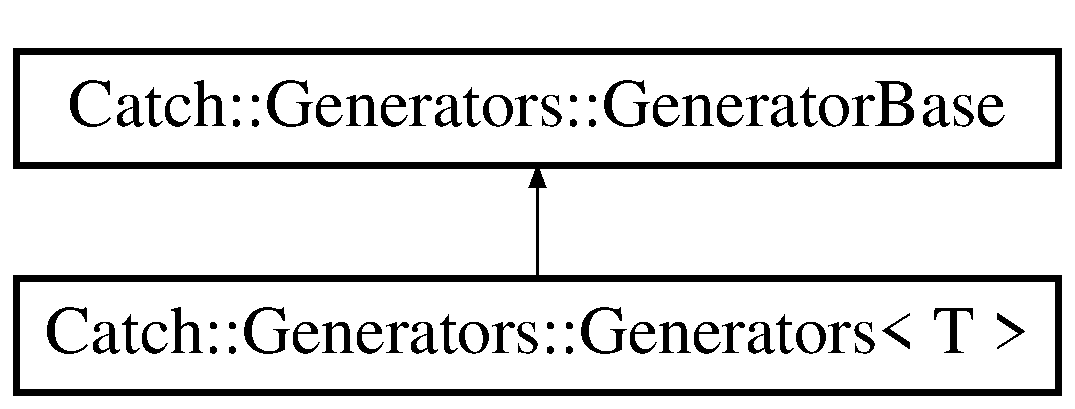
\includegraphics[height=2.000000cm]{class_catch_1_1_generators_1_1_generator_base}
\end{center}
\end{figure}
\subsection*{Public Member Functions}
\begin{DoxyCompactItemize}
\item 
\mbox{\hyperlink{class_catch_1_1_generators_1_1_generator_base_ab003974d458a14acfb48f79e7e8abe21}{Generator\+Base}} (size\+\_\+t \mbox{\hyperlink{class_catch_1_1_generators_1_1_generator_base_a2fb4a5c153f3fdc2708245b40751b487}{size}})
\item 
virtual \mbox{\hyperlink{class_catch_1_1_generators_1_1_generator_base_a6941ab95f6e2a7a2aaa64f0c94b7322c}{$\sim$\+Generator\+Base}} ()
\item 
auto \mbox{\hyperlink{class_catch_1_1_generators_1_1_generator_base_a2fb4a5c153f3fdc2708245b40751b487}{size}} () const -\/$>$ size\+\_\+t
\end{DoxyCompactItemize}
\subsection*{Protected Attributes}
\begin{DoxyCompactItemize}
\item 
size\+\_\+t \mbox{\hyperlink{class_catch_1_1_generators_1_1_generator_base_ac6ab90adfdda9401e2ea03db5b2dfc6a}{m\+\_\+size}} = 0
\end{DoxyCompactItemize}


\subsection{Constructor \& Destructor Documentation}
\mbox{\Hypertarget{class_catch_1_1_generators_1_1_generator_base_ab003974d458a14acfb48f79e7e8abe21}\label{class_catch_1_1_generators_1_1_generator_base_ab003974d458a14acfb48f79e7e8abe21}} 
\index{Catch\+::\+Generators\+::\+Generator\+Base@{Catch\+::\+Generators\+::\+Generator\+Base}!Generator\+Base@{Generator\+Base}}
\index{Generator\+Base@{Generator\+Base}!Catch\+::\+Generators\+::\+Generator\+Base@{Catch\+::\+Generators\+::\+Generator\+Base}}
\subsubsection{\texorpdfstring{Generator\+Base()}{GeneratorBase()}}
{\footnotesize\ttfamily Catch\+::\+Generators\+::\+Generator\+Base\+::\+Generator\+Base (\begin{DoxyParamCaption}\item[{size\+\_\+t}]{size }\end{DoxyParamCaption})\hspace{0.3cm}{\ttfamily [inline]}}

\mbox{\Hypertarget{class_catch_1_1_generators_1_1_generator_base_a6941ab95f6e2a7a2aaa64f0c94b7322c}\label{class_catch_1_1_generators_1_1_generator_base_a6941ab95f6e2a7a2aaa64f0c94b7322c}} 
\index{Catch\+::\+Generators\+::\+Generator\+Base@{Catch\+::\+Generators\+::\+Generator\+Base}!````~Generator\+Base@{$\sim$\+Generator\+Base}}
\index{````~Generator\+Base@{$\sim$\+Generator\+Base}!Catch\+::\+Generators\+::\+Generator\+Base@{Catch\+::\+Generators\+::\+Generator\+Base}}
\subsubsection{\texorpdfstring{$\sim$\+Generator\+Base()}{~GeneratorBase()}}
{\footnotesize\ttfamily virtual Catch\+::\+Generators\+::\+Generator\+Base\+::$\sim$\+Generator\+Base (\begin{DoxyParamCaption}{ }\end{DoxyParamCaption})\hspace{0.3cm}{\ttfamily [virtual]}}



\subsection{Member Function Documentation}
\mbox{\Hypertarget{class_catch_1_1_generators_1_1_generator_base_a2fb4a5c153f3fdc2708245b40751b487}\label{class_catch_1_1_generators_1_1_generator_base_a2fb4a5c153f3fdc2708245b40751b487}} 
\index{Catch\+::\+Generators\+::\+Generator\+Base@{Catch\+::\+Generators\+::\+Generator\+Base}!size@{size}}
\index{size@{size}!Catch\+::\+Generators\+::\+Generator\+Base@{Catch\+::\+Generators\+::\+Generator\+Base}}
\subsubsection{\texorpdfstring{size()}{size()}}
{\footnotesize\ttfamily auto Catch\+::\+Generators\+::\+Generator\+Base\+::size (\begin{DoxyParamCaption}{ }\end{DoxyParamCaption}) const -\/$>$ size\+\_\+t \hspace{0.3cm}{\ttfamily [inline]}}



\subsection{Member Data Documentation}
\mbox{\Hypertarget{class_catch_1_1_generators_1_1_generator_base_ac6ab90adfdda9401e2ea03db5b2dfc6a}\label{class_catch_1_1_generators_1_1_generator_base_ac6ab90adfdda9401e2ea03db5b2dfc6a}} 
\index{Catch\+::\+Generators\+::\+Generator\+Base@{Catch\+::\+Generators\+::\+Generator\+Base}!m\+\_\+size@{m\+\_\+size}}
\index{m\+\_\+size@{m\+\_\+size}!Catch\+::\+Generators\+::\+Generator\+Base@{Catch\+::\+Generators\+::\+Generator\+Base}}
\subsubsection{\texorpdfstring{m\+\_\+size}{m\_size}}
{\footnotesize\ttfamily size\+\_\+t Catch\+::\+Generators\+::\+Generator\+Base\+::m\+\_\+size = 0\hspace{0.3cm}{\ttfamily [protected]}}



The documentation for this class was generated from the following file\+:\begin{DoxyCompactItemize}
\item 
D\+:/kouluhommat/\+Advanced Object-\/\+Oriented Programming/lopputyö/\+Battleship/\+Battleship/\mbox{\hyperlink{catch_8hpp}{catch.\+hpp}}\end{DoxyCompactItemize}

\hypertarget{class_catch_1_1_generators_1_1_generator_randomiser}{}\section{Catch\+:\+:Generators\+:\+:Generator\+Randomiser$<$ T $>$ Class Template Reference}
\label{class_catch_1_1_generators_1_1_generator_randomiser}\index{Catch\+::\+Generators\+::\+Generator\+Randomiser$<$ T $>$@{Catch\+::\+Generators\+::\+Generator\+Randomiser$<$ T $>$}}
Inheritance diagram for Catch\+:\+:Generators\+:\+:Generator\+Randomiser$<$ T $>$\+:\begin{figure}[H]
\begin{center}
\leavevmode
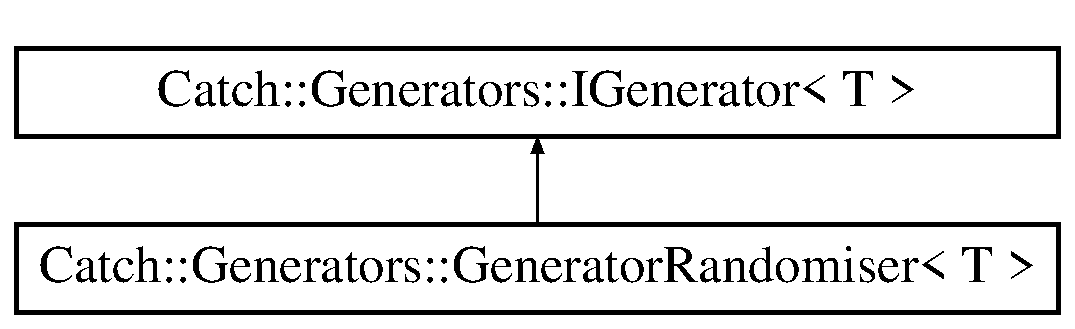
\includegraphics[height=2.000000cm]{class_catch_1_1_generators_1_1_generator_randomiser}
\end{center}
\end{figure}
\subsection*{Public Member Functions}
\begin{DoxyCompactItemize}
\item 
\mbox{\Hypertarget{class_catch_1_1_generators_1_1_generator_randomiser_aba3234a2885baff107766814d10c2efc}\label{class_catch_1_1_generators_1_1_generator_randomiser_aba3234a2885baff107766814d10c2efc}} 
{\bfseries Generator\+Randomiser} (\mbox{\hyperlink{class_catch_1_1_generators_1_1_generator}{Generator}}$<$ T $>$ \&\&base\+Generator, size\+\_\+t number\+Of\+Items)
\item 
\mbox{\Hypertarget{class_catch_1_1_generators_1_1_generator_randomiser_a4ad5de15865727bdaa638863e0969ab4}\label{class_catch_1_1_generators_1_1_generator_randomiser_a4ad5de15865727bdaa638863e0969ab4}} 
auto {\bfseries get} (size\+\_\+t index) const -\/$>$ T override
\end{DoxyCompactItemize}


The documentation for this class was generated from the following file\+:\begin{DoxyCompactItemize}
\item 
D\+:/kouluhommat/\+Advanced Object-\/\+Oriented Programming/lopputyö/\+Battleship/\+Battleship/catch.\+hpp\end{DoxyCompactItemize}

\hypertarget{struct_catch_1_1_generators_1_1_generators}{}\section{Catch\+:\+:Generators\+:\+:Generators$<$ T $>$ Struct Template Reference}
\label{struct_catch_1_1_generators_1_1_generators}\index{Catch\+::\+Generators\+::\+Generators$<$ T $>$@{Catch\+::\+Generators\+::\+Generators$<$ T $>$}}


{\ttfamily \#include $<$catch.\+hpp$>$}

Inheritance diagram for Catch\+:\+:Generators\+:\+:Generators$<$ T $>$\+:\begin{figure}[H]
\begin{center}
\leavevmode
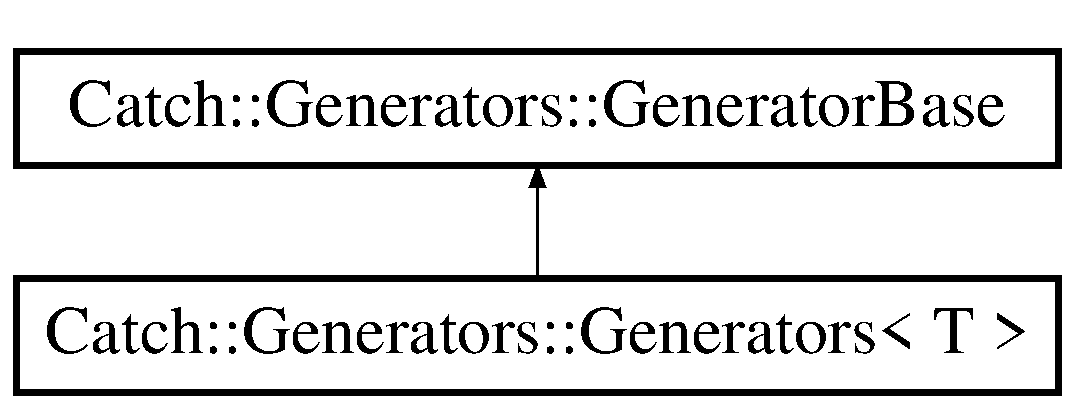
\includegraphics[height=2.000000cm]{struct_catch_1_1_generators_1_1_generators}
\end{center}
\end{figure}
\subsection*{Public Types}
\begin{DoxyCompactItemize}
\item 
using \mbox{\hyperlink{struct_catch_1_1_generators_1_1_generators_aab27f98a577b49532b2ca7556a84286b}{type}} = T
\end{DoxyCompactItemize}
\subsection*{Public Member Functions}
\begin{DoxyCompactItemize}
\item 
\mbox{\hyperlink{struct_catch_1_1_generators_1_1_generators_ad936c563841f7db16a301576c40622e4}{Generators}} ()
\item 
void \mbox{\hyperlink{struct_catch_1_1_generators_1_1_generators_ad708036fa5a9bf0cd1520ce111bc851d}{populate}} (T \&\&val)
\item 
{\footnotesize template$<$typename U $>$ }\\void \mbox{\hyperlink{struct_catch_1_1_generators_1_1_generators_a8ff8b7dda734d1808b644fefc67f4c98}{populate}} (U \&\&val)
\item 
void \mbox{\hyperlink{struct_catch_1_1_generators_1_1_generators_a2155cad48ab03c362483e200d957eefc}{populate}} (\mbox{\hyperlink{class_catch_1_1_generators_1_1_generator}{Generator}}$<$ T $>$ \&\&generator)
\item 
{\footnotesize template$<$typename U , typename... Gs$>$ }\\void \mbox{\hyperlink{struct_catch_1_1_generators_1_1_generators_a4b9680ee28e48e4dc4c4538b5510e649}{populate}} (U \&\&value\+Or\+Generator, Gs... more\+Generators)
\item 
auto \mbox{\hyperlink{struct_catch_1_1_generators_1_1_generators_a1812ebb7d0146d63e3a005e93831afa2}{operator\mbox{[}$\,$\mbox{]}}} (size\+\_\+t index) const -\/$>$ T
\end{DoxyCompactItemize}
\subsection*{Public Attributes}
\begin{DoxyCompactItemize}
\item 
std\+::vector$<$ \mbox{\hyperlink{class_catch_1_1_generators_1_1_generator}{Generator}}$<$ T $>$ $>$ \mbox{\hyperlink{struct_catch_1_1_generators_1_1_generators_a49f1d0e8851a4726bb9981edffe094fa}{m\+\_\+generators}}
\end{DoxyCompactItemize}
\subsection*{Additional Inherited Members}


\subsection{Member Typedef Documentation}
\mbox{\Hypertarget{struct_catch_1_1_generators_1_1_generators_aab27f98a577b49532b2ca7556a84286b}\label{struct_catch_1_1_generators_1_1_generators_aab27f98a577b49532b2ca7556a84286b}} 
\index{Catch\+::\+Generators\+::\+Generators@{Catch\+::\+Generators\+::\+Generators}!type@{type}}
\index{type@{type}!Catch\+::\+Generators\+::\+Generators@{Catch\+::\+Generators\+::\+Generators}}
\subsubsection{\texorpdfstring{type}{type}}
{\footnotesize\ttfamily template$<$typename T $>$ \\
using \mbox{\hyperlink{struct_catch_1_1_generators_1_1_generators}{Catch\+::\+Generators\+::\+Generators}}$<$ T $>$\+::\mbox{\hyperlink{struct_catch_1_1_generators_1_1_generators_aab27f98a577b49532b2ca7556a84286b}{type}} =  T}



\subsection{Constructor \& Destructor Documentation}
\mbox{\Hypertarget{struct_catch_1_1_generators_1_1_generators_ad936c563841f7db16a301576c40622e4}\label{struct_catch_1_1_generators_1_1_generators_ad936c563841f7db16a301576c40622e4}} 
\index{Catch\+::\+Generators\+::\+Generators@{Catch\+::\+Generators\+::\+Generators}!Generators@{Generators}}
\index{Generators@{Generators}!Catch\+::\+Generators\+::\+Generators@{Catch\+::\+Generators\+::\+Generators}}
\subsubsection{\texorpdfstring{Generators()}{Generators()}}
{\footnotesize\ttfamily template$<$typename T $>$ \\
\mbox{\hyperlink{struct_catch_1_1_generators_1_1_generators}{Catch\+::\+Generators\+::\+Generators}}$<$ T $>$\+::\mbox{\hyperlink{struct_catch_1_1_generators_1_1_generators}{Generators}} (\begin{DoxyParamCaption}{ }\end{DoxyParamCaption})\hspace{0.3cm}{\ttfamily [inline]}}



\subsection{Member Function Documentation}
\mbox{\Hypertarget{struct_catch_1_1_generators_1_1_generators_a1812ebb7d0146d63e3a005e93831afa2}\label{struct_catch_1_1_generators_1_1_generators_a1812ebb7d0146d63e3a005e93831afa2}} 
\index{Catch\+::\+Generators\+::\+Generators@{Catch\+::\+Generators\+::\+Generators}!operator\mbox{[}\mbox{]}@{operator[]}}
\index{operator\mbox{[}\mbox{]}@{operator[]}!Catch\+::\+Generators\+::\+Generators@{Catch\+::\+Generators\+::\+Generators}}
\subsubsection{\texorpdfstring{operator[]()}{operator[]()}}
{\footnotesize\ttfamily template$<$typename T $>$ \\
auto \mbox{\hyperlink{struct_catch_1_1_generators_1_1_generators}{Catch\+::\+Generators\+::\+Generators}}$<$ T $>$\+::operator\mbox{[}$\,$\mbox{]} (\begin{DoxyParamCaption}\item[{size\+\_\+t}]{index }\end{DoxyParamCaption}) const -\/$>$ T \hspace{0.3cm}{\ttfamily [inline]}}

\mbox{\Hypertarget{struct_catch_1_1_generators_1_1_generators_ad708036fa5a9bf0cd1520ce111bc851d}\label{struct_catch_1_1_generators_1_1_generators_ad708036fa5a9bf0cd1520ce111bc851d}} 
\index{Catch\+::\+Generators\+::\+Generators@{Catch\+::\+Generators\+::\+Generators}!populate@{populate}}
\index{populate@{populate}!Catch\+::\+Generators\+::\+Generators@{Catch\+::\+Generators\+::\+Generators}}
\subsubsection{\texorpdfstring{populate()}{populate()}\hspace{0.1cm}{\footnotesize\ttfamily [1/4]}}
{\footnotesize\ttfamily template$<$typename T $>$ \\
void \mbox{\hyperlink{struct_catch_1_1_generators_1_1_generators}{Catch\+::\+Generators\+::\+Generators}}$<$ T $>$\+::populate (\begin{DoxyParamCaption}\item[{T \&\&}]{val }\end{DoxyParamCaption})\hspace{0.3cm}{\ttfamily [inline]}}

\mbox{\Hypertarget{struct_catch_1_1_generators_1_1_generators_a8ff8b7dda734d1808b644fefc67f4c98}\label{struct_catch_1_1_generators_1_1_generators_a8ff8b7dda734d1808b644fefc67f4c98}} 
\index{Catch\+::\+Generators\+::\+Generators@{Catch\+::\+Generators\+::\+Generators}!populate@{populate}}
\index{populate@{populate}!Catch\+::\+Generators\+::\+Generators@{Catch\+::\+Generators\+::\+Generators}}
\subsubsection{\texorpdfstring{populate()}{populate()}\hspace{0.1cm}{\footnotesize\ttfamily [2/4]}}
{\footnotesize\ttfamily template$<$typename T $>$ \\
template$<$typename U $>$ \\
void \mbox{\hyperlink{struct_catch_1_1_generators_1_1_generators}{Catch\+::\+Generators\+::\+Generators}}$<$ T $>$\+::populate (\begin{DoxyParamCaption}\item[{U \&\&}]{val }\end{DoxyParamCaption})\hspace{0.3cm}{\ttfamily [inline]}}

\mbox{\Hypertarget{struct_catch_1_1_generators_1_1_generators_a2155cad48ab03c362483e200d957eefc}\label{struct_catch_1_1_generators_1_1_generators_a2155cad48ab03c362483e200d957eefc}} 
\index{Catch\+::\+Generators\+::\+Generators@{Catch\+::\+Generators\+::\+Generators}!populate@{populate}}
\index{populate@{populate}!Catch\+::\+Generators\+::\+Generators@{Catch\+::\+Generators\+::\+Generators}}
\subsubsection{\texorpdfstring{populate()}{populate()}\hspace{0.1cm}{\footnotesize\ttfamily [3/4]}}
{\footnotesize\ttfamily template$<$typename T $>$ \\
void \mbox{\hyperlink{struct_catch_1_1_generators_1_1_generators}{Catch\+::\+Generators\+::\+Generators}}$<$ T $>$\+::populate (\begin{DoxyParamCaption}\item[{\mbox{\hyperlink{class_catch_1_1_generators_1_1_generator}{Generator}}$<$ T $>$ \&\&}]{generator }\end{DoxyParamCaption})\hspace{0.3cm}{\ttfamily [inline]}}

\mbox{\Hypertarget{struct_catch_1_1_generators_1_1_generators_a4b9680ee28e48e4dc4c4538b5510e649}\label{struct_catch_1_1_generators_1_1_generators_a4b9680ee28e48e4dc4c4538b5510e649}} 
\index{Catch\+::\+Generators\+::\+Generators@{Catch\+::\+Generators\+::\+Generators}!populate@{populate}}
\index{populate@{populate}!Catch\+::\+Generators\+::\+Generators@{Catch\+::\+Generators\+::\+Generators}}
\subsubsection{\texorpdfstring{populate()}{populate()}\hspace{0.1cm}{\footnotesize\ttfamily [4/4]}}
{\footnotesize\ttfamily template$<$typename T $>$ \\
template$<$typename U , typename... Gs$>$ \\
void \mbox{\hyperlink{struct_catch_1_1_generators_1_1_generators}{Catch\+::\+Generators\+::\+Generators}}$<$ T $>$\+::populate (\begin{DoxyParamCaption}\item[{U \&\&}]{value\+Or\+Generator,  }\item[{Gs...}]{more\+Generators }\end{DoxyParamCaption})\hspace{0.3cm}{\ttfamily [inline]}}



\subsection{Member Data Documentation}
\mbox{\Hypertarget{struct_catch_1_1_generators_1_1_generators_a49f1d0e8851a4726bb9981edffe094fa}\label{struct_catch_1_1_generators_1_1_generators_a49f1d0e8851a4726bb9981edffe094fa}} 
\index{Catch\+::\+Generators\+::\+Generators@{Catch\+::\+Generators\+::\+Generators}!m\+\_\+generators@{m\+\_\+generators}}
\index{m\+\_\+generators@{m\+\_\+generators}!Catch\+::\+Generators\+::\+Generators@{Catch\+::\+Generators\+::\+Generators}}
\subsubsection{\texorpdfstring{m\+\_\+generators}{m\_generators}}
{\footnotesize\ttfamily template$<$typename T $>$ \\
std\+::vector$<$\mbox{\hyperlink{class_catch_1_1_generators_1_1_generator}{Generator}}$<$T$>$ $>$ \mbox{\hyperlink{struct_catch_1_1_generators_1_1_generators}{Catch\+::\+Generators\+::\+Generators}}$<$ T $>$\+::m\+\_\+generators}



The documentation for this struct was generated from the following file\+:\begin{DoxyCompactItemize}
\item 
D\+:/kouluhommat/\+Advanced Object-\/\+Oriented Programming/lopputyö/\+Battleship/\+Battleship/\mbox{\hyperlink{catch_8hpp}{catch.\+hpp}}\end{DoxyCompactItemize}

\hypertarget{class_hard_player}{}\section{Hard\+Player Class Reference}
\label{class_hard_player}\index{Hard\+Player@{Hard\+Player}}


{\ttfamily \#include $<$Hard\+Player.\+h$>$}

Inheritance diagram for Hard\+Player\+:\begin{figure}[H]
\begin{center}
\leavevmode
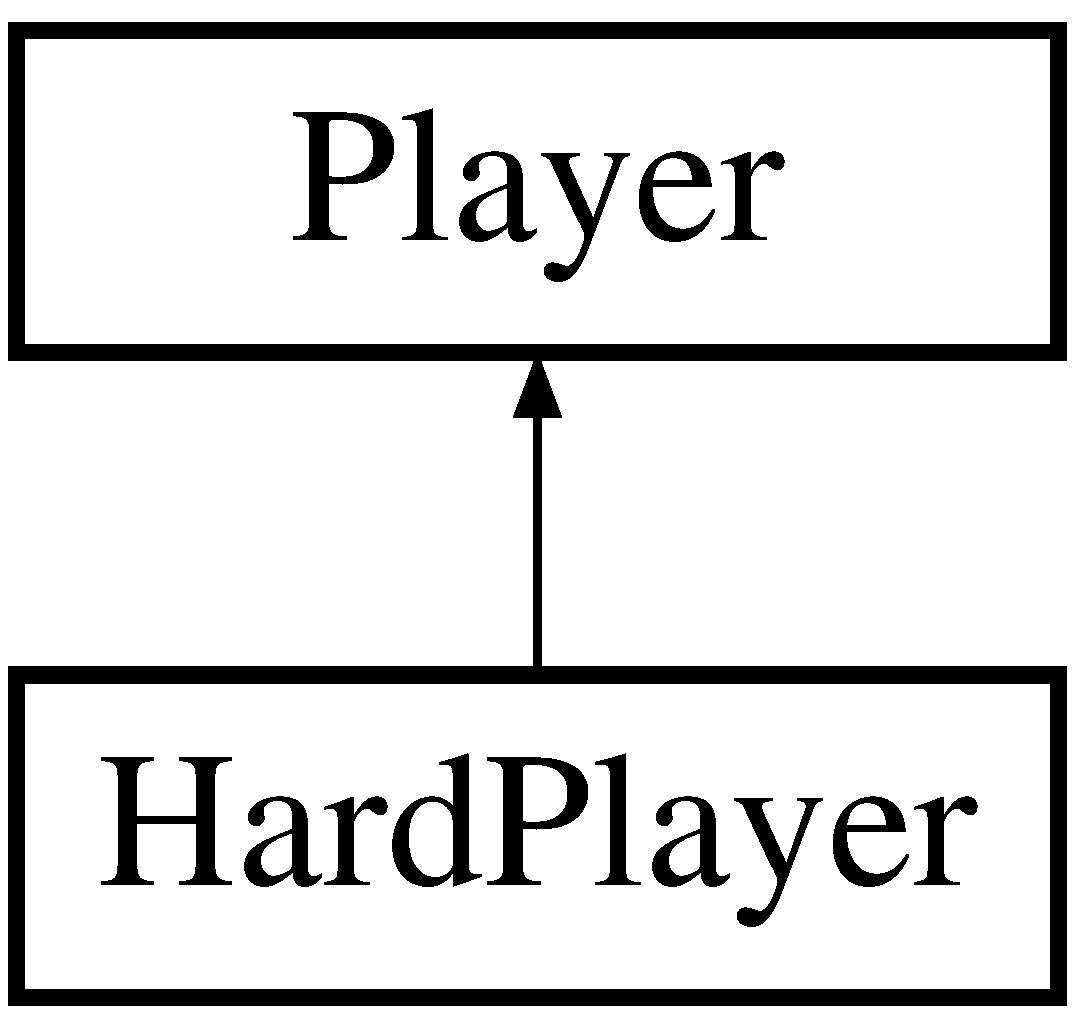
\includegraphics[height=2.000000cm]{class_hard_player}
\end{center}
\end{figure}
\subsection*{Public Member Functions}
\begin{DoxyCompactItemize}
\item 
\mbox{\hyperlink{class_player}{Player}} $\ast$ \mbox{\hyperlink{class_hard_player_aa435bcb65ee8b3aea7553196c95fc4e1}{create}} (std\+::string nm, const \mbox{\hyperlink{class_game}{Game}} \&g) override
\item 
\mbox{\hyperlink{class_hard_player_a40d564084e88021b21324672bf67b169}{Hard\+Player}} (std\+::string nm, const \mbox{\hyperlink{class_game}{Game}} \&g)
\begin{DoxyCompactList}\small\item\em Constructor for hard bot. \end{DoxyCompactList}\item 
virtual bool \mbox{\hyperlink{class_hard_player_a27d0ad3353eba585d7a93d2092036f98}{place\+Ships}} (\mbox{\hyperlink{class_board}{Board}} \&b)
\begin{DoxyCompactList}\small\item\em Destructor for hard player. \end{DoxyCompactList}\item 
virtual \mbox{\hyperlink{class_point}{Point}} \mbox{\hyperlink{class_hard_player_ae1d21325a648a88f1bf51f2b0b286190}{recommend}} ()
\item 
virtual void \mbox{\hyperlink{class_hard_player_aa8977ca3294daf996707bd0ff434d69e}{record\+Result}} (\mbox{\hyperlink{class_point}{Point}} p, bool valid\+Shot, bool hit, bool destroyed, int ship\+ID)
\item 
virtual void \mbox{\hyperlink{class_hard_player_a986175fb966099ac5fe39950e18799ae}{record\+Opponent}} (\mbox{\hyperlink{class_point}{Point}} p)
\item 
\mbox{\Hypertarget{class_hard_player_a063d9f4071b687339fbc134239771ef3}\label{class_hard_player_a063d9f4071b687339fbc134239771ef3}} 
virtual bool {\bfseries get\+State} () const
\item 
\mbox{\Hypertarget{class_hard_player_aa25afded558192bd39d8d2c1b2a8209a}\label{class_hard_player_aa25afded558192bd39d8d2c1b2a8209a}} 
virtual void {\bfseries change\+State} (bool state)
\item 
\mbox{\Hypertarget{class_hard_player_ad86f7d42434ae5526d7a1ca4ea65b51a}\label{class_hard_player_ad86f7d42434ae5526d7a1ca4ea65b51a}} 
virtual \mbox{\hyperlink{class_point}{Point}} {\bfseries get\+LastP} () const
\item 
virtual bool \mbox{\hyperlink{class_hard_player_a8107a94c8db7d5f1023dbeeddfaaedb2}{already\+Shot}} (\mbox{\hyperlink{class_point}{Point}} p)
\item 
virtual void \mbox{\hyperlink{class_hard_player_a77c82c1a36c9e956fdab98837ed888e5}{add\+Point}} (\mbox{\hyperlink{class_point}{Point}} p)
\item 
bool \mbox{\hyperlink{class_hard_player_aec6ff0ed3ef8f47ac46d374cff89e6be}{hard\+Helper}} (\mbox{\hyperlink{class_board}{Board}} \&b, int ship\+ID, int c, int track)
\begin{DoxyCompactList}\small\item\em Method for helping hard bot\textquotesingle{}s operations. \end{DoxyCompactList}\item 
bool \mbox{\hyperlink{class_hard_player_aebad1f5ad6f9ac20eb4f1ca639088c7b}{check\+Ships}} (\mbox{\hyperlink{class_point}{Point}} p, \mbox{\hyperlink{_globals_8h_a224b9163917ac32fc95a60d8c1eec3aa}{Direction}} d, int ship\+ID)
\begin{DoxyCompactList}\small\item\em Method for checking ships. \end{DoxyCompactList}\item 
void \mbox{\hyperlink{class_hard_player_a9358a28f7f0e618d3c98aba7b135e6a8}{record\+Ship}} (\mbox{\hyperlink{class_point}{Point}} p, \mbox{\hyperlink{_globals_8h_a224b9163917ac32fc95a60d8c1eec3aa}{Direction}} d, int ship\+ID)
\begin{DoxyCompactList}\small\item\em Method for recording ships. \end{DoxyCompactList}\item 
bool \mbox{\hyperlink{class_hard_player_a91cdd6239e111ea02bff561f6a3a0c41}{close\+By}} (\mbox{\hyperlink{class_point}{Point}} p)
\begin{DoxyCompactList}\small\item\em Method for checking target\textquotesingle{}s that are close by. \end{DoxyCompactList}\end{DoxyCompactItemize}


\subsection{Detailed Description}
\mbox{\hyperlink{class_hard_player}{Hard\+Player}}\+: declaration for player class that\textquotesingle{}s controlled by hard bot 

\subsection{Constructor \& Destructor Documentation}
\mbox{\Hypertarget{class_hard_player_a40d564084e88021b21324672bf67b169}\label{class_hard_player_a40d564084e88021b21324672bf67b169}} 
\index{Hard\+Player@{Hard\+Player}!Hard\+Player@{Hard\+Player}}
\index{Hard\+Player@{Hard\+Player}!Hard\+Player@{Hard\+Player}}
\subsubsection{\texorpdfstring{Hard\+Player()}{HardPlayer()}}
{\footnotesize\ttfamily Hard\+Player\+::\+Hard\+Player (\begin{DoxyParamCaption}\item[{std\+::string}]{nm,  }\item[{const \mbox{\hyperlink{class_game}{Game}} \&}]{g }\end{DoxyParamCaption})\hspace{0.3cm}{\ttfamily [inline]}}



Constructor for hard bot. 

Loops through game\textquotesingle{}s rows

Loops through games columns

$<$ Clears screen 

\subsection{Member Function Documentation}
\mbox{\Hypertarget{class_hard_player_a77c82c1a36c9e956fdab98837ed888e5}\label{class_hard_player_a77c82c1a36c9e956fdab98837ed888e5}} 
\index{Hard\+Player@{Hard\+Player}!add\+Point@{add\+Point}}
\index{add\+Point@{add\+Point}!Hard\+Player@{Hard\+Player}}
\subsubsection{\texorpdfstring{add\+Point()}{addPoint()}}
{\footnotesize\ttfamily void Hard\+Player\+::add\+Point (\begin{DoxyParamCaption}\item[{\mbox{\hyperlink{class_point}{Point}}}]{p }\end{DoxyParamCaption})\hspace{0.3cm}{\ttfamily [virtual]}}

Method for adding target location to shots 
\begin{DoxyParams}{Parameters}
{\em p} & \mbox{\hyperlink{class_point}{Point}} containing targeted cell \\
\hline
\end{DoxyParams}
\mbox{\Hypertarget{class_hard_player_a8107a94c8db7d5f1023dbeeddfaaedb2}\label{class_hard_player_a8107a94c8db7d5f1023dbeeddfaaedb2}} 
\index{Hard\+Player@{Hard\+Player}!already\+Shot@{already\+Shot}}
\index{already\+Shot@{already\+Shot}!Hard\+Player@{Hard\+Player}}
\subsubsection{\texorpdfstring{already\+Shot()}{alreadyShot()}}
{\footnotesize\ttfamily bool Hard\+Player\+::already\+Shot (\begin{DoxyParamCaption}\item[{\mbox{\hyperlink{class_point}{Point}}}]{p }\end{DoxyParamCaption})\hspace{0.3cm}{\ttfamily [virtual]}}

Method for checking if player has already shot targeted location 
\begin{DoxyParams}{Parameters}
{\em p} & \mbox{\hyperlink{class_point}{Point}} containing target cell \\
\hline
\end{DoxyParams}
Checks if target is OoB

Loops through number of shots

Checks if shots contain targeted cell \mbox{\Hypertarget{class_hard_player_aebad1f5ad6f9ac20eb4f1ca639088c7b}\label{class_hard_player_aebad1f5ad6f9ac20eb4f1ca639088c7b}} 
\index{Hard\+Player@{Hard\+Player}!check\+Ships@{check\+Ships}}
\index{check\+Ships@{check\+Ships}!Hard\+Player@{Hard\+Player}}
\subsubsection{\texorpdfstring{check\+Ships()}{checkShips()}}
{\footnotesize\ttfamily bool Hard\+Player\+::check\+Ships (\begin{DoxyParamCaption}\item[{\mbox{\hyperlink{class_point}{Point}}}]{p,  }\item[{\mbox{\hyperlink{_globals_8h_a224b9163917ac32fc95a60d8c1eec3aa}{Direction}}}]{d,  }\item[{int}]{ship\+ID }\end{DoxyParamCaption})}



Method for checking ships. 

Method for checking ship\textquotesingle{}s location 
\begin{DoxyParams}{Parameters}
{\em p} & \mbox{\hyperlink{class_point}{Point}} containing target cell \\
\hline
{\em d} & Direction of the ship \\
\hline
{\em ship\+ID} & Integer containing ship\textquotesingle{}s id \\
\hline
\end{DoxyParams}
Checks if ship\textquotesingle{}s direction is horizontal

Loops through ship length by ship\textquotesingle{}s ID

Checks if target cell is valid and contains space next to it

Checks if ship has been tracked on location

Checks if target cell is valid and contains space next to it

Checks if my\+Ships contains a ship mark next to it

Checks if target cell is valid for the ship

Checks if ship has been tracked on location

Checks if target cell is valid and has a column next to it

Checks if my\+Ships contains a ship symbol next to it

Checks if target is valid and has a column next to it

Checks if my\+Ships contains a ship symbol next to it

Checks if target cell is valid for the ship

Checks if ship has been tracked on location

$<$ \mbox{\hyperlink{class_ship}{Ship}} is vertical ~\newline
~\newline
~\newline
~\newline
~\newline
~\newline
~\newline
~\newline
~\newline
~\newline
~\newline
~\newline
~\newline
 Loops through ship length by ship\textquotesingle{}s ID

Checks if target cell is valid and has a row it

Checks if there is a ship under it

Checks if target cell is valid and has a row under it

Checks if there is a ship under it

Checks if target cell is valid

Checks if ship has been tracked on location

Checks if target cell is valid and has a row on top of it

Checks if rows above it contain a ship

Checks if target cell is valid

Checks if ship has been tracked on location

Checks if target cell is valid for the ship

Checks if ship has been tracked on location \mbox{\Hypertarget{class_hard_player_a91cdd6239e111ea02bff561f6a3a0c41}\label{class_hard_player_a91cdd6239e111ea02bff561f6a3a0c41}} 
\index{Hard\+Player@{Hard\+Player}!close\+By@{close\+By}}
\index{close\+By@{close\+By}!Hard\+Player@{Hard\+Player}}
\subsubsection{\texorpdfstring{close\+By()}{closeBy()}}
{\footnotesize\ttfamily bool Hard\+Player\+::close\+By (\begin{DoxyParamCaption}\item[{\mbox{\hyperlink{class_point}{Point}}}]{p }\end{DoxyParamCaption})}



Method for checking target\textquotesingle{}s that are close by. 

Method for checking if there are targets close by 
\begin{DoxyParams}{Parameters}
{\em p} & \mbox{\hyperlink{class_point}{Point}} containing targeted cell \\
\hline
\end{DoxyParams}
Loops through number of shots \mbox{\Hypertarget{class_hard_player_aa435bcb65ee8b3aea7553196c95fc4e1}\label{class_hard_player_aa435bcb65ee8b3aea7553196c95fc4e1}} 
\index{Hard\+Player@{Hard\+Player}!create@{create}}
\index{create@{create}!Hard\+Player@{Hard\+Player}}
\subsubsection{\texorpdfstring{create()}{create()}}
{\footnotesize\ttfamily \mbox{\hyperlink{class_player}{Player}}$\ast$ Hard\+Player\+::create (\begin{DoxyParamCaption}\item[{std\+::string}]{nm,  }\item[{const \mbox{\hyperlink{class_game}{Game}} \&}]{g }\end{DoxyParamCaption})\hspace{0.3cm}{\ttfamily [inline]}, {\ttfamily [override]}, {\ttfamily [virtual]}}

Pure virtual method for creating a player 
\begin{DoxyParams}{Parameters}
{\em nm} & string containing player\textquotesingle{}s name \\
\hline
{\em g} & reference to game object \\
\hline
\end{DoxyParams}


Implements \mbox{\hyperlink{class_player_a9b9133f3347894da1416953048cecdb2}{Player}}.

\mbox{\Hypertarget{class_hard_player_aec6ff0ed3ef8f47ac46d374cff89e6be}\label{class_hard_player_aec6ff0ed3ef8f47ac46d374cff89e6be}} 
\index{Hard\+Player@{Hard\+Player}!hard\+Helper@{hard\+Helper}}
\index{hard\+Helper@{hard\+Helper}!Hard\+Player@{Hard\+Player}}
\subsubsection{\texorpdfstring{hard\+Helper()}{hardHelper()}}
{\footnotesize\ttfamily bool Hard\+Player\+::hard\+Helper (\begin{DoxyParamCaption}\item[{\mbox{\hyperlink{class_board}{Board}} \&}]{b,  }\item[{int}]{ship\+ID,  }\item[{int}]{c,  }\item[{int}]{track }\end{DoxyParamCaption})}



Method for helping hard bot\textquotesingle{}s operations. 

Method for helping hard bot\textquotesingle{}s operations 
\begin{DoxyParams}{Parameters}
{\em b} & reference to game board \\
\hline
{\em ship\+ID} & integer containing ship\textquotesingle{}s id \\
\hline
{\em c} & integer containing count \\
\hline
{\em track} & integer containing track of ships \\
\hline
\end{DoxyParams}
Checks if all the ship\textquotesingle{}s have been placed

Checks if we just need to place some ships

Top left

$<$ Top right

$<$ Bottom left

$<$ Bottom right

$<$ Anywhere

Switch case for random direction

$<$ Place vertical ship ~\newline
~\newline
~\newline
~\newline
~\newline
~\newline
~\newline
~\newline
~\newline
~\newline
~\newline
~\newline
~\newline
~\newline
 Checks if ship can\textquotesingle{}t be placed

$<$ increase track

Checks tracked ships

$<$ Removes ship

$<$ Increase track

$<$ Change direction to vertical

$<$ Place horizontal ship ~\newline
~\newline
~\newline
~\newline
~\newline
~\newline
~\newline
 Checks if ship can\textquotesingle{}t be placed

$<$ Increase track

checks tracked ship

$<$ Removes ship

$<$ Increase track

$<$ Change direction to horizontal

$<$ Place ship into grid to track it \mbox{\Hypertarget{class_hard_player_a27d0ad3353eba585d7a93d2092036f98}\label{class_hard_player_a27d0ad3353eba585d7a93d2092036f98}} 
\index{Hard\+Player@{Hard\+Player}!place\+Ships@{place\+Ships}}
\index{place\+Ships@{place\+Ships}!Hard\+Player@{Hard\+Player}}
\subsubsection{\texorpdfstring{place\+Ships()}{placeShips()}}
{\footnotesize\ttfamily bool Hard\+Player\+::place\+Ships (\begin{DoxyParamCaption}\item[{\mbox{\hyperlink{class_board}{Board}} \&}]{b }\end{DoxyParamCaption})\hspace{0.3cm}{\ttfamily [virtual]}}



Destructor for hard player. 

Method for placing ships 
\begin{DoxyParams}{Parameters}
{\em b} & reference to game board \\
\hline
\end{DoxyParams}


Implements \mbox{\hyperlink{class_player_ab89c1180c7314d3e19bcf4b2bed2e02a}{Player}}.

\mbox{\Hypertarget{class_hard_player_ae1d21325a648a88f1bf51f2b0b286190}\label{class_hard_player_ae1d21325a648a88f1bf51f2b0b286190}} 
\index{Hard\+Player@{Hard\+Player}!recommend@{recommend}}
\index{recommend@{recommend}!Hard\+Player@{Hard\+Player}}
\subsubsection{\texorpdfstring{recommend()}{recommend()}}
{\footnotesize\ttfamily \mbox{\hyperlink{class_point}{Point}} Hard\+Player\+::recommend (\begin{DoxyParamCaption}{ }\end{DoxyParamCaption})\hspace{0.3cm}{\ttfamily [virtual]}}

Method for recommending attack $<$ Ford figuring out next shot

Checks if state is 1

$<$ Get random point ~\newline
~\newline
~\newline
~\newline
~\newline
~\newline
~\newline
~\newline
~\newline
~\newline
~\newline
~\newline
~\newline
~\newline
~\newline
~\newline
~\newline
~\newline
~\newline
~\newline
~\newline
~\newline
~\newline
~\newline
~\newline
~\newline
~\newline
~\newline
~\newline
~\newline
~\newline
~\newline
~\newline
~\newline
~\newline
~\newline
~\newline
~\newline
~\newline
~\newline
~\newline
~\newline
~\newline
 Checks random point has already been shot

Checks if number of shots is under 30 and there is a ship close to target cell

$<$ Return random cell

$<$ State is 2 ~\newline
~\newline
~\newline
~\newline
~\newline
~\newline
~\newline
~\newline
~\newline
~\newline
~\newline
~\newline
~\newline
~\newline
~\newline
~\newline
~\newline
~\newline
~\newline
~\newline
~\newline
~\newline
~\newline
~\newline
~\newline
~\newline
~\newline
~\newline
~\newline
~\newline
~\newline
~\newline
~\newline
~\newline
~\newline
~\newline
~\newline
~\newline
~\newline
 Checks if hits since state change is ore than 1

Checks if ship is horizontal

Checks if ship is heading to right

$<$ Shoot to the right side next

$<$ Ships is probably heading left

$<$ Shoot to the left side next

Checks if we have reached the end of grid

Loop while we are still targeting the end

$<$ Go back left ~\newline
~\newline
~\newline
~\newline
~\newline
~\newline
~\newline
~\newline
~\newline
~\newline
~\newline
~\newline
~\newline
~\newline
~\newline
~\newline
~\newline
~\newline
~\newline
~\newline
~\newline
~\newline
~\newline
~\newline
~\newline
~\newline
~\newline
~\newline
~\newline
~\newline
 Checks if target column is less than 0

$<$ Checks if we have reached the end of grid ~\newline
~\newline
~\newline
~\newline
~\newline
~\newline
~\newline
~\newline
~\newline
~\newline
~\newline
~\newline
~\newline
~\newline
~\newline
~\newline
~\newline
~\newline
~\newline
~\newline
~\newline
~\newline
~\newline
~\newline
~\newline
~\newline
~\newline
~\newline
 Loop while we are still targeting the end

$<$ Go back right ~\newline
~\newline
~\newline
~\newline
~\newline
~\newline
~\newline
~\newline
~\newline
~\newline
~\newline
~\newline
~\newline
~\newline
~\newline
~\newline
~\newline
~\newline
~\newline
~\newline
~\newline
~\newline
~\newline
~\newline
~\newline
~\newline
 Checks if target column is more than game\textquotesingle{}s columns

$<$ Checks if ship is vertical ~\newline
~\newline
~\newline
~\newline
~\newline
~\newline
~\newline
~\newline
~\newline
~\newline
~\newline
~\newline
~\newline
~\newline
~\newline
~\newline
~\newline
~\newline
~\newline
~\newline
~\newline
~\newline
~\newline
~\newline
 Checks if ship is heading up

$<$ Shoot up next

$<$ \mbox{\hyperlink{class_ship}{Ship}} is heading down

$<$ Shoot down next

Check if we have reached the end of grid

Loop while we are still targeting the end

$<$ Go back up ~\newline
~\newline
~\newline
~\newline
~\newline
~\newline
~\newline
~\newline
~\newline
~\newline
~\newline
~\newline
~\newline
~\newline
~\newline
~\newline
~\newline
 Check if rows are less than 0

$<$ Check if we have reached the end of grid ~\newline
~\newline
~\newline
~\newline
~\newline
~\newline
~\newline
~\newline
~\newline
~\newline
~\newline
~\newline
~\newline
~\newline
~\newline
 Loop while we are still targeting the end

$<$ Go back down ~\newline
~\newline
~\newline
~\newline
~\newline
~\newline
~\newline
~\newline
~\newline
~\newline
~\newline
~\newline
~\newline
 If rows is less than game\textquotesingle{}s rows

$<$ Target has been hit, circle around

$<$ Look down

Check if target hasn\textquotesingle{}t been already shot

$<$ Look left ~\newline
~\newline
~\newline
~\newline
~\newline
~\newline
~\newline
~\newline
 Check if target hasn\textquotesingle{}t been already shot

$<$ Look up

Check if target hasn\textquotesingle{}t been already shot

$<$ Look right ~\newline
~\newline
~\newline
~\newline
 If target hasn\textquotesingle{}t already been shot

$<$ Just shoot somewhere

Checks if target has already been shot

Check if target has already been shot 

Implements \mbox{\hyperlink{class_player_a2cc7a83d11158eafd8d49d4b9f23ce56}{Player}}.

\mbox{\Hypertarget{class_hard_player_a986175fb966099ac5fe39950e18799ae}\label{class_hard_player_a986175fb966099ac5fe39950e18799ae}} 
\index{Hard\+Player@{Hard\+Player}!record\+Opponent@{record\+Opponent}}
\index{record\+Opponent@{record\+Opponent}!Hard\+Player@{Hard\+Player}}
\subsubsection{\texorpdfstring{record\+Opponent()}{recordOpponent()}}
{\footnotesize\ttfamily void Hard\+Player\+::record\+Opponent (\begin{DoxyParamCaption}\item[{\mbox{\hyperlink{class_point}{Point}}}]{p }\end{DoxyParamCaption})\hspace{0.3cm}{\ttfamily [virtual]}}

Method for recording opponent\textquotesingle{}s attacks 
\begin{DoxyParams}{Parameters}
{\em p} & \mbox{\hyperlink{class_point}{Point}} containing targeted cell \\
\hline
\end{DoxyParams}


Implements \mbox{\hyperlink{class_player_a768e14edee61e208e6fd295cdd72a49c}{Player}}.

\mbox{\Hypertarget{class_hard_player_aa8977ca3294daf996707bd0ff434d69e}\label{class_hard_player_aa8977ca3294daf996707bd0ff434d69e}} 
\index{Hard\+Player@{Hard\+Player}!record\+Result@{record\+Result}}
\index{record\+Result@{record\+Result}!Hard\+Player@{Hard\+Player}}
\subsubsection{\texorpdfstring{record\+Result()}{recordResult()}}
{\footnotesize\ttfamily void Hard\+Player\+::record\+Result (\begin{DoxyParamCaption}\item[{\mbox{\hyperlink{class_point}{Point}}}]{p,  }\item[{bool}]{valid\+Shot,  }\item[{bool}]{hit,  }\item[{bool}]{destroyed,  }\item[{int}]{ship\+ID }\end{DoxyParamCaption})\hspace{0.3cm}{\ttfamily [virtual]}}

Method for recording attack result 
\begin{DoxyParams}{Parameters}
{\em p} & \mbox{\hyperlink{class_point}{Point}} containing target cell \\
\hline
{\em valid\+Shot} & boolean for checking if shot is valid \\
\hline
{\em hit} & boolean for checking if shot was hit \\
\hline
{\em destroyed} & boolean for checking if ship was destroyed \\
\hline
{\em ship\+ID} & Integer that contains ship\textquotesingle{}s ID \\
\hline
\end{DoxyParams}
Checks if shot wasn\textquotesingle{}t valid

Checks if target hasn\textquotesingle{}t been already shot

$<$ Add the point to the array

Checks if target was hit

$<$ Adds target point to the vector

$<$ Increase hits since last state change

$<$ Changes state to 2

Checks if ship was destroyed

$<$ Reset hits since last state change

$<$ Return back to state 1 

Implements \mbox{\hyperlink{class_player_a368527cfefaac58dc942b32658f977ed}{Player}}.

\mbox{\Hypertarget{class_hard_player_a9358a28f7f0e618d3c98aba7b135e6a8}\label{class_hard_player_a9358a28f7f0e618d3c98aba7b135e6a8}} 
\index{Hard\+Player@{Hard\+Player}!record\+Ship@{record\+Ship}}
\index{record\+Ship@{record\+Ship}!Hard\+Player@{Hard\+Player}}
\subsubsection{\texorpdfstring{record\+Ship()}{recordShip()}}
{\footnotesize\ttfamily void Hard\+Player\+::record\+Ship (\begin{DoxyParamCaption}\item[{\mbox{\hyperlink{class_point}{Point}}}]{p,  }\item[{\mbox{\hyperlink{_globals_8h_a224b9163917ac32fc95a60d8c1eec3aa}{Direction}}}]{d,  }\item[{int}]{ship\+ID }\end{DoxyParamCaption})}



Method for recording ships. 

Method for placing a ship on a grid to track it 
\begin{DoxyParams}{Parameters}
{\em p} & \mbox{\hyperlink{class_point}{Point}} containing target cell \\
\hline
{\em d} & Direction of ship \\
\hline
{\em ship\+ID} & Integer containing ship\textquotesingle{}s id \\
\hline
\end{DoxyParams}
Checks if direction is horizontal

Loops through ship length by ID

$<$ Direction is vertical ~\newline
 Loops through ship length by ID 

The documentation for this class was generated from the following files\+:\begin{DoxyCompactItemize}
\item 
D\+:/kouluhommat/\+Advanced Object-\/\+Oriented Programming/lopputyö/\+Battleship/\+Battleship/\mbox{\hyperlink{_hard_player_8h}{Hard\+Player.\+h}}\item 
D\+:/kouluhommat/\+Advanced Object-\/\+Oriented Programming/lopputyö/\+Battleship/\+Battleship/\mbox{\hyperlink{_player_8cpp}{Player.\+cpp}}\end{DoxyCompactItemize}

\hypertarget{class_human_player}{}\section{Human\+Player Class Reference}
\label{class_human_player}\index{Human\+Player@{Human\+Player}}


{\ttfamily \#include $<$Player.\+h$>$}

Inheritance diagram for Human\+Player\+:\begin{figure}[H]
\begin{center}
\leavevmode
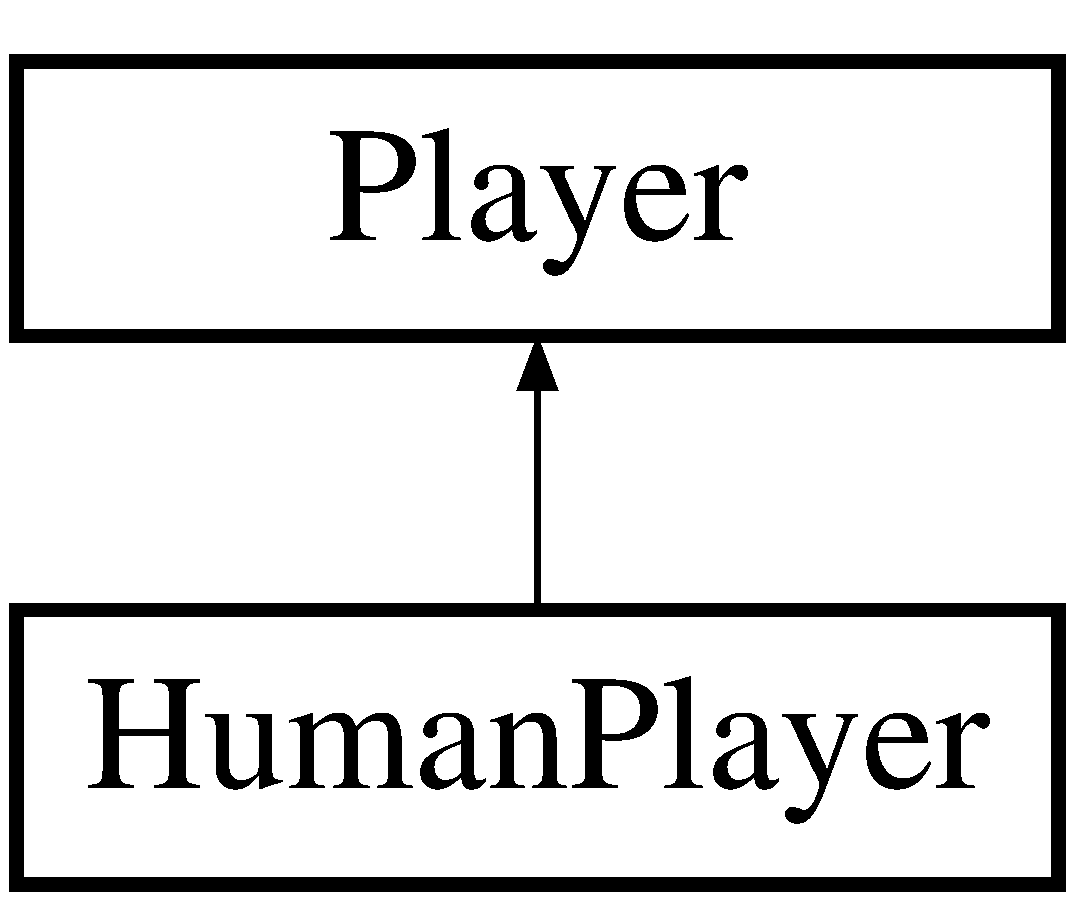
\includegraphics[height=2.000000cm]{class_human_player}
\end{center}
\end{figure}
\subsection*{Public Member Functions}
\begin{DoxyCompactItemize}
\item 
\mbox{\hyperlink{class_player}{Player}} $\ast$ \mbox{\hyperlink{class_human_player_ac369ccb03a62b40dcf3dc157841a965e}{create}} (std\+::string nm, const \mbox{\hyperlink{class_game}{Game}} \&g)
\item 
\mbox{\Hypertarget{class_human_player_a443ff25b201959966555c0902a10e19c}\label{class_human_player_a443ff25b201959966555c0902a10e19c}} 
{\bfseries Human\+Player} (std\+::string nm, const \mbox{\hyperlink{class_game}{Game}} \&g)
\item 
\mbox{\Hypertarget{class_human_player_acecbe621447504a013c2a763aaba05fa}\label{class_human_player_acecbe621447504a013c2a763aaba05fa}} 
virtual bool \mbox{\hyperlink{class_human_player_acecbe621447504a013c2a763aaba05fa}{human}} () const
\begin{DoxyCompactList}\small\item\em Destructor for human player. \end{DoxyCompactList}\item 
virtual bool \mbox{\hyperlink{class_human_player_ae9315a3c66f6b2f2bf4d1ebb09669aff}{place\+Ships}} (\mbox{\hyperlink{class_board}{Board}} \&b)
\item 
virtual \mbox{\hyperlink{class_point}{Point}} \mbox{\hyperlink{class_human_player_a718f16f3ddeeb34c9f2e93cf1d805b46}{recommend}} ()
\item 
virtual void \mbox{\hyperlink{class_human_player_a19be81244b7a1c88a3ca89d207055b6e}{record\+Result}} (\mbox{\hyperlink{class_point}{Point}} p, bool valid\+Shot, bool hit, bool destroyed, int ship\+ID)
\item 
virtual void \mbox{\hyperlink{class_human_player_a16b18f42e02d7c8d1f0971ce5e91595f}{record\+Opponent}} (\mbox{\hyperlink{class_point}{Point}} p)
\end{DoxyCompactItemize}


\subsection{Detailed Description}
\mbox{\hyperlink{class_human_player}{Human\+Player}}\+: implementation for player class that\textquotesingle{}s controlled by human 

\subsection{Member Function Documentation}
\mbox{\Hypertarget{class_human_player_ac369ccb03a62b40dcf3dc157841a965e}\label{class_human_player_ac369ccb03a62b40dcf3dc157841a965e}} 
\index{Human\+Player@{Human\+Player}!create@{create}}
\index{create@{create}!Human\+Player@{Human\+Player}}
\subsubsection{\texorpdfstring{create()}{create()}}
{\footnotesize\ttfamily \mbox{\hyperlink{class_player}{Player}}$\ast$ Human\+Player\+::create (\begin{DoxyParamCaption}\item[{std\+::string}]{nm,  }\item[{const \mbox{\hyperlink{class_game}{Game}} \&}]{g }\end{DoxyParamCaption})\hspace{0.3cm}{\ttfamily [inline]}, {\ttfamily [virtual]}}

Pure virtual method for creating a player 
\begin{DoxyParams}{Parameters}
{\em nm} & string containing player\textquotesingle{}s name \\
\hline
{\em g} & reference to game object \\
\hline
\end{DoxyParams}


Implements \mbox{\hyperlink{class_player_a9b9133f3347894da1416953048cecdb2}{Player}}.

\mbox{\Hypertarget{class_human_player_ae9315a3c66f6b2f2bf4d1ebb09669aff}\label{class_human_player_ae9315a3c66f6b2f2bf4d1ebb09669aff}} 
\index{Human\+Player@{Human\+Player}!place\+Ships@{place\+Ships}}
\index{place\+Ships@{place\+Ships}!Human\+Player@{Human\+Player}}
\subsubsection{\texorpdfstring{place\+Ships()}{placeShips()}}
{\footnotesize\ttfamily bool Human\+Player\+::place\+Ships (\begin{DoxyParamCaption}\item[{\mbox{\hyperlink{class_board}{Board}} \&}]{b }\end{DoxyParamCaption})\hspace{0.3cm}{\ttfamily [virtual]}}

Method for placing ships 
\begin{DoxyParams}{Parameters}
{\em b} & reference to board \\
\hline
\end{DoxyParams}
Loops through ships

Checks if choice is 1, then ship\textquotesingle{}s direction is horizontal

$<$ Checks if choice is 2, then ship\textquotesingle{}s direction is vertical

$<$ Not a valid choice

$<$ Get row and column from user input ~\newline
~\newline
~\newline
~\newline
~\newline
~\newline
~\newline
~\newline
~\newline
~\newline
~\newline
~\newline
~\newline
~\newline
~\newline
~\newline
~\newline
~\newline
~\newline
~\newline
~\newline
 Checks if ship isn\textquotesingle{}t placed into valid cell

Checks if choice is 1, then ship\textquotesingle{}s direction is horizontal

$<$ Checks if choice is 2, then ship\textquotesingle{}s direction is vertical

$<$ Not a valid direction

$<$ Get row and column from user input ~\newline
~\newline
~\newline
~\newline
~\newline
~\newline
~\newline
~\newline
~\newline
~\newline
~\newline
~\newline
~\newline
~\newline
~\newline
~\newline
 Checks if ship is placed into valid location

Checks if choice is 1 then ship is horizontal

$<$ Checks if choice is 2 then ship is vertical

$<$ Direction is not valid

$<$ Get row and column from user input

$<$ Checks if ship is placed into valid cell

Checks if choice is 1 then ship is horizontal

$<$ Checks if choice is 2 then ship is vertical

$<$ Direction is not valid

$<$ Get rows and columns from user input ~\newline
~\newline
~\newline
~\newline
~\newline
~\newline
 Checks if ship is placed into valid cell

Checks if choice is 1 then ship is horizontal

$<$ Checks if choice is 2 then ship is vertical

$<$ Direction is not valid

$<$ Get row and column from user input ~\newline
 Checks if ship is placed into valid cell 

Implements \mbox{\hyperlink{class_player_ab89c1180c7314d3e19bcf4b2bed2e02a}{Player}}.

\mbox{\Hypertarget{class_human_player_a718f16f3ddeeb34c9f2e93cf1d805b46}\label{class_human_player_a718f16f3ddeeb34c9f2e93cf1d805b46}} 
\index{Human\+Player@{Human\+Player}!recommend@{recommend}}
\index{recommend@{recommend}!Human\+Player@{Human\+Player}}
\subsubsection{\texorpdfstring{recommend()}{recommend()}}
{\footnotesize\ttfamily \mbox{\hyperlink{class_point}{Point}} Human\+Player\+::recommend (\begin{DoxyParamCaption}{ }\end{DoxyParamCaption})\hspace{0.3cm}{\ttfamily [virtual]}}

Method for getting user input for target cell 

Implements \mbox{\hyperlink{class_player_a2cc7a83d11158eafd8d49d4b9f23ce56}{Player}}.

\mbox{\Hypertarget{class_human_player_a16b18f42e02d7c8d1f0971ce5e91595f}\label{class_human_player_a16b18f42e02d7c8d1f0971ce5e91595f}} 
\index{Human\+Player@{Human\+Player}!record\+Opponent@{record\+Opponent}}
\index{record\+Opponent@{record\+Opponent}!Human\+Player@{Human\+Player}}
\subsubsection{\texorpdfstring{record\+Opponent()}{recordOpponent()}}
{\footnotesize\ttfamily void Human\+Player\+::record\+Opponent (\begin{DoxyParamCaption}\item[{\mbox{\hyperlink{class_point}{Point}}}]{p }\end{DoxyParamCaption})\hspace{0.3cm}{\ttfamily [virtual]}}

Method for recording opponent\textquotesingle{}s result 
\begin{DoxyParams}{Parameters}
{\em p} & \mbox{\hyperlink{class_point}{Point}} containing targetted cell \\
\hline
\end{DoxyParams}


Implements \mbox{\hyperlink{class_player_a768e14edee61e208e6fd295cdd72a49c}{Player}}.

\mbox{\Hypertarget{class_human_player_a19be81244b7a1c88a3ca89d207055b6e}\label{class_human_player_a19be81244b7a1c88a3ca89d207055b6e}} 
\index{Human\+Player@{Human\+Player}!record\+Result@{record\+Result}}
\index{record\+Result@{record\+Result}!Human\+Player@{Human\+Player}}
\subsubsection{\texorpdfstring{record\+Result()}{recordResult()}}
{\footnotesize\ttfamily void Human\+Player\+::record\+Result (\begin{DoxyParamCaption}\item[{\mbox{\hyperlink{class_point}{Point}}}]{p,  }\item[{bool}]{valid\+Shot,  }\item[{bool}]{hit,  }\item[{bool}]{destroyed,  }\item[{int}]{ship\+ID }\end{DoxyParamCaption})\hspace{0.3cm}{\ttfamily [virtual]}}

Method for recording result 
\begin{DoxyParams}{Parameters}
{\em p} & \mbox{\hyperlink{class_point}{Point}} where player attacked \\
\hline
{\em valid\+Shot} & boolean that checks if shot is valid \\
\hline
{\em hit} & boolean that checks if shot hit \\
\hline
{\em destroyed} & boolean that checks if ship was destroyed \\
\hline
{\em ship\+ID} & integer containing ship ID \\
\hline
\end{DoxyParams}


Implements \mbox{\hyperlink{class_player_a368527cfefaac58dc942b32658f977ed}{Player}}.



The documentation for this class was generated from the following files\+:\begin{DoxyCompactItemize}
\item 
D\+:/kouluhommat/\+Advanced Object-\/\+Oriented Programming/lopputyö/\+Battleship/\+Battleship/\mbox{\hyperlink{_player_8h}{Player.\+h}}\item 
D\+:/kouluhommat/\+Advanced Object-\/\+Oriented Programming/lopputyö/\+Battleship/\+Battleship/\mbox{\hyperlink{_player_8cpp}{Player.\+cpp}}\end{DoxyCompactItemize}

\hypertarget{struct_catch_1_1_i_exception_translator}{}\section{Catch\+:\+:I\+Exception\+Translator Struct Reference}
\label{struct_catch_1_1_i_exception_translator}\index{Catch\+::\+I\+Exception\+Translator@{Catch\+::\+I\+Exception\+Translator}}


{\ttfamily \#include $<$catch.\+hpp$>$}

\subsection*{Public Member Functions}
\begin{DoxyCompactItemize}
\item 
virtual \mbox{\hyperlink{struct_catch_1_1_i_exception_translator_afa00bb6258c07591df472aadae05783f}{$\sim$\+I\+Exception\+Translator}} ()
\item 
virtual std\+::string \mbox{\hyperlink{struct_catch_1_1_i_exception_translator_a2a554b96ed5ed411e7c796b6b42837a5}{translate}} (Exception\+Translators\+::const\+\_\+iterator it, Exception\+Translators\+::const\+\_\+iterator it\+End) const =0
\end{DoxyCompactItemize}


\subsection{Constructor \& Destructor Documentation}
\mbox{\Hypertarget{struct_catch_1_1_i_exception_translator_afa00bb6258c07591df472aadae05783f}\label{struct_catch_1_1_i_exception_translator_afa00bb6258c07591df472aadae05783f}} 
\index{Catch\+::\+I\+Exception\+Translator@{Catch\+::\+I\+Exception\+Translator}!````~I\+Exception\+Translator@{$\sim$\+I\+Exception\+Translator}}
\index{````~I\+Exception\+Translator@{$\sim$\+I\+Exception\+Translator}!Catch\+::\+I\+Exception\+Translator@{Catch\+::\+I\+Exception\+Translator}}
\subsubsection{\texorpdfstring{$\sim$\+I\+Exception\+Translator()}{~IExceptionTranslator()}}
{\footnotesize\ttfamily virtual Catch\+::\+I\+Exception\+Translator\+::$\sim$\+I\+Exception\+Translator (\begin{DoxyParamCaption}{ }\end{DoxyParamCaption})\hspace{0.3cm}{\ttfamily [virtual]}}



\subsection{Member Function Documentation}
\mbox{\Hypertarget{struct_catch_1_1_i_exception_translator_a2a554b96ed5ed411e7c796b6b42837a5}\label{struct_catch_1_1_i_exception_translator_a2a554b96ed5ed411e7c796b6b42837a5}} 
\index{Catch\+::\+I\+Exception\+Translator@{Catch\+::\+I\+Exception\+Translator}!translate@{translate}}
\index{translate@{translate}!Catch\+::\+I\+Exception\+Translator@{Catch\+::\+I\+Exception\+Translator}}
\subsubsection{\texorpdfstring{translate()}{translate()}}
{\footnotesize\ttfamily virtual std\+::string Catch\+::\+I\+Exception\+Translator\+::translate (\begin{DoxyParamCaption}\item[{Exception\+Translators\+::const\+\_\+iterator}]{it,  }\item[{Exception\+Translators\+::const\+\_\+iterator}]{it\+End }\end{DoxyParamCaption}) const\hspace{0.3cm}{\ttfamily [pure virtual]}}



The documentation for this struct was generated from the following file\+:\begin{DoxyCompactItemize}
\item 
D\+:/kouluhommat/\+Advanced Object-\/\+Oriented Programming/lopputyö/\+Battleship/\+Battleship/\mbox{\hyperlink{catch_8hpp}{catch.\+hpp}}\end{DoxyCompactItemize}

\hypertarget{struct_catch_1_1_i_exception_translator_registry}{}\section{Catch\+:\+:I\+Exception\+Translator\+Registry Struct Reference}
\label{struct_catch_1_1_i_exception_translator_registry}\index{Catch\+::\+I\+Exception\+Translator\+Registry@{Catch\+::\+I\+Exception\+Translator\+Registry}}
\subsection*{Public Member Functions}
\begin{DoxyCompactItemize}
\item 
\mbox{\Hypertarget{struct_catch_1_1_i_exception_translator_registry_af76ae8c331a17f2a94c9720bc0d686bb}\label{struct_catch_1_1_i_exception_translator_registry_af76ae8c331a17f2a94c9720bc0d686bb}} 
virtual std\+::string {\bfseries translate\+Active\+Exception} () const =0
\end{DoxyCompactItemize}


The documentation for this struct was generated from the following file\+:\begin{DoxyCompactItemize}
\item 
D\+:/kouluhommat/\+Advanced Object-\/\+Oriented Programming/lopputyö/\+Battleship/\+Battleship/catch.\+hpp\end{DoxyCompactItemize}

\hypertarget{struct_catch_1_1_generators_1_1_i_generator}{}\section{Catch\+:\+:Generators\+:\+:I\+Generator$<$ T $>$ Struct Template Reference}
\label{struct_catch_1_1_generators_1_1_i_generator}\index{Catch\+::\+Generators\+::\+I\+Generator$<$ T $>$@{Catch\+::\+Generators\+::\+I\+Generator$<$ T $>$}}


{\ttfamily \#include $<$catch.\+hpp$>$}

Inheritance diagram for Catch\+:\+:Generators\+:\+:I\+Generator$<$ T $>$\+:\begin{figure}[H]
\begin{center}
\leavevmode
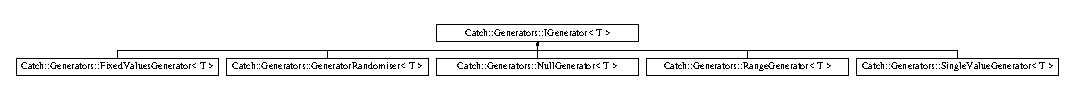
\includegraphics[height=0.783217cm]{struct_catch_1_1_generators_1_1_i_generator}
\end{center}
\end{figure}
\subsection*{Public Member Functions}
\begin{DoxyCompactItemize}
\item 
virtual \mbox{\hyperlink{struct_catch_1_1_generators_1_1_i_generator_a7d877bd8144e71d402347b227c909ffb}{$\sim$\+I\+Generator}} ()
\item 
virtual auto \mbox{\hyperlink{struct_catch_1_1_generators_1_1_i_generator_a737a89eb0bff02e580e36c59fb0d1171}{get}} (size\+\_\+t index) const -\/$>$ T=0
\end{DoxyCompactItemize}


\subsection{Constructor \& Destructor Documentation}
\mbox{\Hypertarget{struct_catch_1_1_generators_1_1_i_generator_a7d877bd8144e71d402347b227c909ffb}\label{struct_catch_1_1_generators_1_1_i_generator_a7d877bd8144e71d402347b227c909ffb}} 
\index{Catch\+::\+Generators\+::\+I\+Generator@{Catch\+::\+Generators\+::\+I\+Generator}!````~I\+Generator@{$\sim$\+I\+Generator}}
\index{````~I\+Generator@{$\sim$\+I\+Generator}!Catch\+::\+Generators\+::\+I\+Generator@{Catch\+::\+Generators\+::\+I\+Generator}}
\subsubsection{\texorpdfstring{$\sim$\+I\+Generator()}{~IGenerator()}}
{\footnotesize\ttfamily template$<$typename T $>$ \\
virtual \mbox{\hyperlink{struct_catch_1_1_generators_1_1_i_generator}{Catch\+::\+Generators\+::\+I\+Generator}}$<$ T $>$\+::$\sim$\mbox{\hyperlink{struct_catch_1_1_generators_1_1_i_generator}{I\+Generator}} (\begin{DoxyParamCaption}{ }\end{DoxyParamCaption})\hspace{0.3cm}{\ttfamily [inline]}, {\ttfamily [virtual]}}



\subsection{Member Function Documentation}
\mbox{\Hypertarget{struct_catch_1_1_generators_1_1_i_generator_a737a89eb0bff02e580e36c59fb0d1171}\label{struct_catch_1_1_generators_1_1_i_generator_a737a89eb0bff02e580e36c59fb0d1171}} 
\index{Catch\+::\+Generators\+::\+I\+Generator@{Catch\+::\+Generators\+::\+I\+Generator}!get@{get}}
\index{get@{get}!Catch\+::\+Generators\+::\+I\+Generator@{Catch\+::\+Generators\+::\+I\+Generator}}
\subsubsection{\texorpdfstring{get()}{get()}}
{\footnotesize\ttfamily template$<$typename T $>$ \\
virtual auto \mbox{\hyperlink{struct_catch_1_1_generators_1_1_i_generator}{Catch\+::\+Generators\+::\+I\+Generator}}$<$ T $>$\+::get (\begin{DoxyParamCaption}\item[{size\+\_\+t}]{index }\end{DoxyParamCaption}) const -\/$>$  T\hspace{0.3cm}{\ttfamily [pure virtual]}}



Implemented in \mbox{\hyperlink{class_catch_1_1_generators_1_1_generator_randomiser_a4ad5de15865727bdaa638863e0969ab4}{Catch\+::\+Generators\+::\+Generator\+Randomiser$<$ T $>$}}, \mbox{\hyperlink{struct_catch_1_1_generators_1_1_null_generator_a17a2cc82d644e97afded4017c7a062ef}{Catch\+::\+Generators\+::\+Null\+Generator$<$ T $>$}}, \mbox{\hyperlink{class_catch_1_1_generators_1_1_range_generator_a78f7f624b7545823d1a683ebf2ac00e7}{Catch\+::\+Generators\+::\+Range\+Generator$<$ T $>$}}, \mbox{\hyperlink{class_catch_1_1_generators_1_1_fixed_values_generator_a3ed654a5860c170dbe7b01487b83253d}{Catch\+::\+Generators\+::\+Fixed\+Values\+Generator$<$ T $>$}}, and \mbox{\hyperlink{class_catch_1_1_generators_1_1_single_value_generator_ad03af3fe263136425595bfd2eec84209}{Catch\+::\+Generators\+::\+Single\+Value\+Generator$<$ T $>$}}.



The documentation for this struct was generated from the following file\+:\begin{DoxyCompactItemize}
\item 
D\+:/kouluhommat/\+Advanced Object-\/\+Oriented Programming/lopputyö/\+Battleship/\+Battleship/\mbox{\hyperlink{catch_8hpp}{catch.\+hpp}}\end{DoxyCompactItemize}

\hypertarget{struct_catch_1_1_i_generator_tracker}{}\section{Catch\+:\+:I\+Generator\+Tracker Struct Reference}
\label{struct_catch_1_1_i_generator_tracker}\index{Catch\+::\+I\+Generator\+Tracker@{Catch\+::\+I\+Generator\+Tracker}}
\subsection*{Public Member Functions}
\begin{DoxyCompactItemize}
\item 
\mbox{\Hypertarget{struct_catch_1_1_i_generator_tracker_ae88084f9af27c8b9a5d5775b9c148498}\label{struct_catch_1_1_i_generator_tracker_ae88084f9af27c8b9a5d5775b9c148498}} 
virtual auto {\bfseries has\+Generator} () const -\/$>$ bool=0
\item 
\mbox{\Hypertarget{struct_catch_1_1_i_generator_tracker_a23be942fc51672598bfa02c678c3078a}\label{struct_catch_1_1_i_generator_tracker_a23be942fc51672598bfa02c678c3078a}} 
virtual auto {\bfseries get\+Generator} () const -\/$>$ Generators\+::\+Generator\+Base\+Ptr const \&=0
\item 
\mbox{\Hypertarget{struct_catch_1_1_i_generator_tracker_a9945eff42219edc5a7071eebd8b0419e}\label{struct_catch_1_1_i_generator_tracker_a9945eff42219edc5a7071eebd8b0419e}} 
virtual void {\bfseries set\+Generator} (Generators\+::\+Generator\+Base\+Ptr \&\&generator)=0
\item 
\mbox{\Hypertarget{struct_catch_1_1_i_generator_tracker_a2922f0d8bc7a732079eadbda78e30f79}\label{struct_catch_1_1_i_generator_tracker_a2922f0d8bc7a732079eadbda78e30f79}} 
virtual auto {\bfseries get\+Index} () const -\/$>$ std\+::size\+\_\+t=0
\end{DoxyCompactItemize}


The documentation for this struct was generated from the following file\+:\begin{DoxyCompactItemize}
\item 
D\+:/kouluhommat/\+Advanced Object-\/\+Oriented Programming/lopputyö/\+Battleship/\+Battleship/catch.\+hpp\end{DoxyCompactItemize}

\hypertarget{struct_catch_1_1_i_mutable_registry_hub}{}\section{Catch\+:\+:I\+Mutable\+Registry\+Hub Struct Reference}
\label{struct_catch_1_1_i_mutable_registry_hub}\index{Catch\+::\+I\+Mutable\+Registry\+Hub@{Catch\+::\+I\+Mutable\+Registry\+Hub}}
\subsection*{Public Member Functions}
\begin{DoxyCompactItemize}
\item 
\mbox{\Hypertarget{struct_catch_1_1_i_mutable_registry_hub_a1c0ac202ac31ee9f88e8ff5cbac4b243}\label{struct_catch_1_1_i_mutable_registry_hub_a1c0ac202ac31ee9f88e8ff5cbac4b243}} 
virtual void {\bfseries register\+Reporter} (std\+::string const \&name, I\+Reporter\+Factory\+Ptr const \&factory)=0
\item 
\mbox{\Hypertarget{struct_catch_1_1_i_mutable_registry_hub_abd892a133f85581fd00ee75bb379ca56}\label{struct_catch_1_1_i_mutable_registry_hub_abd892a133f85581fd00ee75bb379ca56}} 
virtual void {\bfseries register\+Listener} (I\+Reporter\+Factory\+Ptr const \&factory)=0
\item 
\mbox{\Hypertarget{struct_catch_1_1_i_mutable_registry_hub_a11b85c6744d88c9f83fe16ad4a8dd451}\label{struct_catch_1_1_i_mutable_registry_hub_a11b85c6744d88c9f83fe16ad4a8dd451}} 
virtual void {\bfseries register\+Test} (\mbox{\hyperlink{class_catch_1_1_test_case}{Test\+Case}} const \&test\+Info)=0
\item 
\mbox{\Hypertarget{struct_catch_1_1_i_mutable_registry_hub_ae6825365102693cf7707db022a2c2b49}\label{struct_catch_1_1_i_mutable_registry_hub_ae6825365102693cf7707db022a2c2b49}} 
virtual void {\bfseries register\+Translator} (const \mbox{\hyperlink{struct_catch_1_1_i_exception_translator}{I\+Exception\+Translator}} $\ast$translator)=0
\item 
\mbox{\Hypertarget{struct_catch_1_1_i_mutable_registry_hub_abf2e386b6f94f615719ada711adbf822}\label{struct_catch_1_1_i_mutable_registry_hub_abf2e386b6f94f615719ada711adbf822}} 
virtual void {\bfseries register\+Tag\+Alias} (std\+::string const \&alias, std\+::string const \&tag, \mbox{\hyperlink{struct_catch_1_1_source_line_info}{Source\+Line\+Info}} const \&line\+Info)=0
\item 
\mbox{\Hypertarget{struct_catch_1_1_i_mutable_registry_hub_a72a7d5386851ac3200f8da794a009c86}\label{struct_catch_1_1_i_mutable_registry_hub_a72a7d5386851ac3200f8da794a009c86}} 
virtual void {\bfseries register\+Startup\+Exception} () noexcept=0
\end{DoxyCompactItemize}


The documentation for this struct was generated from the following file\+:\begin{DoxyCompactItemize}
\item 
D\+:/kouluhommat/\+Advanced Object-\/\+Oriented Programming/lopputyö/\+Battleship/\+Battleship/catch.\+hpp\end{DoxyCompactItemize}

\hypertarget{struct_catch_1_1_i_registry_hub}{}\section{Catch\+:\+:I\+Registry\+Hub Struct Reference}
\label{struct_catch_1_1_i_registry_hub}\index{Catch\+::\+I\+Registry\+Hub@{Catch\+::\+I\+Registry\+Hub}}
\subsection*{Public Member Functions}
\begin{DoxyCompactItemize}
\item 
\mbox{\Hypertarget{struct_catch_1_1_i_registry_hub_a55534563f7ecf7e20ec1e37285ebe54d}\label{struct_catch_1_1_i_registry_hub_a55534563f7ecf7e20ec1e37285ebe54d}} 
virtual I\+Reporter\+Registry const  \& {\bfseries get\+Reporter\+Registry} () const =0
\item 
\mbox{\Hypertarget{struct_catch_1_1_i_registry_hub_af4f6255f0c0f8f1f179fa9d7d4843076}\label{struct_catch_1_1_i_registry_hub_af4f6255f0c0f8f1f179fa9d7d4843076}} 
virtual \mbox{\hyperlink{struct_catch_1_1_i_test_case_registry}{I\+Test\+Case\+Registry}} const  \& {\bfseries get\+Test\+Case\+Registry} () const =0
\item 
\mbox{\Hypertarget{struct_catch_1_1_i_registry_hub_a3c511b1d33e5a6d95c333a0ff387df1a}\label{struct_catch_1_1_i_registry_hub_a3c511b1d33e5a6d95c333a0ff387df1a}} 
virtual I\+Tag\+Alias\+Registry const  \& {\bfseries get\+Tag\+Alias\+Registry} () const =0
\item 
\mbox{\Hypertarget{struct_catch_1_1_i_registry_hub_a48347c170d9c583af73027a27b2f0bd4}\label{struct_catch_1_1_i_registry_hub_a48347c170d9c583af73027a27b2f0bd4}} 
virtual \mbox{\hyperlink{struct_catch_1_1_i_exception_translator_registry}{I\+Exception\+Translator\+Registry}} const  \& {\bfseries get\+Exception\+Translator\+Registry} () const =0
\item 
\mbox{\Hypertarget{struct_catch_1_1_i_registry_hub_a00281210628e6c616aca1d3e0d84db04}\label{struct_catch_1_1_i_registry_hub_a00281210628e6c616aca1d3e0d84db04}} 
virtual Startup\+Exception\+Registry const  \& {\bfseries get\+Startup\+Exception\+Registry} () const =0
\end{DoxyCompactItemize}


The documentation for this struct was generated from the following file\+:\begin{DoxyCompactItemize}
\item 
D\+:/kouluhommat/\+Advanced Object-\/\+Oriented Programming/lopputyö/\+Battleship/\+Battleship/catch.\+hpp\end{DoxyCompactItemize}

\hypertarget{struct_catch_1_1_i_result_capture}{}\section{Catch\+:\+:I\+Result\+Capture Struct Reference}
\label{struct_catch_1_1_i_result_capture}\index{Catch\+::\+I\+Result\+Capture@{Catch\+::\+I\+Result\+Capture}}


{\ttfamily \#include $<$catch.\+hpp$>$}

\subsection*{Public Member Functions}
\begin{DoxyCompactItemize}
\item 
virtual \mbox{\hyperlink{struct_catch_1_1_i_result_capture_a3bd16719d6772b7470887fc36c6d0808}{$\sim$\+I\+Result\+Capture}} ()
\item 
virtual bool \mbox{\hyperlink{struct_catch_1_1_i_result_capture_a5b76ed52badcb64cf374202e12b81a03}{section\+Started}} (\mbox{\hyperlink{struct_catch_1_1_section_info}{Section\+Info}} const \&section\+Info, \mbox{\hyperlink{struct_catch_1_1_counts}{Counts}} \&assertions)=0
\item 
virtual void \mbox{\hyperlink{struct_catch_1_1_i_result_capture_a4e152bc43dc0933684e31fa67a58195d}{section\+Ended}} (\mbox{\hyperlink{struct_catch_1_1_section_end_info}{Section\+End\+Info}} const \&end\+Info)=0
\item 
virtual void \mbox{\hyperlink{struct_catch_1_1_i_result_capture_afcc71eef8ca821ae132cced4a2be6988}{section\+Ended\+Early}} (\mbox{\hyperlink{struct_catch_1_1_section_end_info}{Section\+End\+Info}} const \&end\+Info)=0
\item 
virtual auto \mbox{\hyperlink{struct_catch_1_1_i_result_capture_ab020d111e29ad1cabe1227dcfda712ef}{acquire\+Generator\+Tracker}} (\mbox{\hyperlink{struct_catch_1_1_source_line_info}{Source\+Line\+Info}} const \&line\+Info) -\/$>$ \mbox{\hyperlink{struct_catch_1_1_i_generator_tracker}{I\+Generator\+Tracker}} \&=0
\item 
virtual void \mbox{\hyperlink{struct_catch_1_1_i_result_capture_a264ae12330c74b2daae41715a30d51bf}{benchmark\+Starting}} (Benchmark\+Info const \&info)=0
\item 
virtual void \mbox{\hyperlink{struct_catch_1_1_i_result_capture_a6e5e64f9d94211a888249012ab6cc7fb}{benchmark\+Ended}} (Benchmark\+Stats const \&stats)=0
\item 
virtual void \mbox{\hyperlink{struct_catch_1_1_i_result_capture_a91d154c1e087e383dcde5aad95cb6a05}{push\+Scoped\+Message}} (\mbox{\hyperlink{struct_catch_1_1_message_info}{Message\+Info}} const \&message)=0
\item 
virtual void \mbox{\hyperlink{struct_catch_1_1_i_result_capture_a42bcb13276706bf8c3ce081ce16d37fd}{pop\+Scoped\+Message}} (\mbox{\hyperlink{struct_catch_1_1_message_info}{Message\+Info}} const \&message)=0
\item 
virtual void \mbox{\hyperlink{struct_catch_1_1_i_result_capture_a48559e6598ba9474b903697b69c769b2}{handle\+Fatal\+Error\+Condition}} (\mbox{\hyperlink{class_catch_1_1_string_ref}{String\+Ref}} message)=0
\item 
virtual void \mbox{\hyperlink{struct_catch_1_1_i_result_capture_a59a2b05391e464954575d2afb6d5d607}{handle\+Expr}} (\mbox{\hyperlink{struct_catch_1_1_assertion_info}{Assertion\+Info}} const \&info, \mbox{\hyperlink{struct_catch_1_1_i_transient_expression}{I\+Transient\+Expression}} const \&expr, \mbox{\hyperlink{struct_catch_1_1_assertion_reaction}{Assertion\+Reaction}} \&reaction)=0
\item 
virtual void \mbox{\hyperlink{struct_catch_1_1_i_result_capture_a21788ebc64571abf322b80c8cc51794d}{handle\+Message}} (\mbox{\hyperlink{struct_catch_1_1_assertion_info}{Assertion\+Info}} const \&info, \mbox{\hyperlink{struct_catch_1_1_result_was_a624e1ee3661fcf6094ceef1f654601ef}{Result\+Was\+::\+Of\+Type}} result\+Type, \mbox{\hyperlink{class_catch_1_1_string_ref}{String\+Ref}} const \&message, \mbox{\hyperlink{struct_catch_1_1_assertion_reaction}{Assertion\+Reaction}} \&reaction)=0
\item 
virtual void \mbox{\hyperlink{struct_catch_1_1_i_result_capture_a6382ed20486e2d9a020da971c6d5c53d}{handle\+Unexpected\+Exception\+Not\+Thrown}} (\mbox{\hyperlink{struct_catch_1_1_assertion_info}{Assertion\+Info}} const \&info, \mbox{\hyperlink{struct_catch_1_1_assertion_reaction}{Assertion\+Reaction}} \&reaction)=0
\item 
virtual void \mbox{\hyperlink{struct_catch_1_1_i_result_capture_afc97bc69829185222f955ebeef97adfe}{handle\+Unexpected\+Inflight\+Exception}} (\mbox{\hyperlink{struct_catch_1_1_assertion_info}{Assertion\+Info}} const \&info, std\+::string const \&message, \mbox{\hyperlink{struct_catch_1_1_assertion_reaction}{Assertion\+Reaction}} \&reaction)=0
\item 
virtual void \mbox{\hyperlink{struct_catch_1_1_i_result_capture_a89b89372eb09cc44f8dcad363de6157d}{handle\+Incomplete}} (\mbox{\hyperlink{struct_catch_1_1_assertion_info}{Assertion\+Info}} const \&info)=0
\item 
virtual void \mbox{\hyperlink{struct_catch_1_1_i_result_capture_ab7dbdf8aa28427119583e24dbb302c63}{handle\+Non\+Expr}} (\mbox{\hyperlink{struct_catch_1_1_assertion_info}{Assertion\+Info}} const \&info, \mbox{\hyperlink{struct_catch_1_1_result_was_a624e1ee3661fcf6094ceef1f654601ef}{Result\+Was\+::\+Of\+Type}} result\+Type, \mbox{\hyperlink{struct_catch_1_1_assertion_reaction}{Assertion\+Reaction}} \&reaction)=0
\item 
virtual bool \mbox{\hyperlink{struct_catch_1_1_i_result_capture_a973435fbdcb2f6f07a0ec5719a01e956}{last\+Assertion\+Passed}} ()=0
\item 
virtual void \mbox{\hyperlink{struct_catch_1_1_i_result_capture_a9b0ef2cb071e9a9dc6ec1b533026aea7}{assertion\+Passed}} ()=0
\item 
virtual std\+::string \mbox{\hyperlink{struct_catch_1_1_i_result_capture_aea1617f4a84cc648246aa3ed6918b5bf}{get\+Current\+Test\+Name}} () const =0
\item 
virtual const Assertion\+Result $\ast$ \mbox{\hyperlink{struct_catch_1_1_i_result_capture_ab18872c89fab97405a56e9c6a4919736}{get\+Last\+Result}} () const =0
\item 
virtual void \mbox{\hyperlink{struct_catch_1_1_i_result_capture_ae63ecec95db4c236c63ecf616f483810}{exception\+Early\+Reported}} ()=0
\end{DoxyCompactItemize}


\subsection{Constructor \& Destructor Documentation}
\mbox{\Hypertarget{struct_catch_1_1_i_result_capture_a3bd16719d6772b7470887fc36c6d0808}\label{struct_catch_1_1_i_result_capture_a3bd16719d6772b7470887fc36c6d0808}} 
\index{Catch\+::\+I\+Result\+Capture@{Catch\+::\+I\+Result\+Capture}!````~I\+Result\+Capture@{$\sim$\+I\+Result\+Capture}}
\index{````~I\+Result\+Capture@{$\sim$\+I\+Result\+Capture}!Catch\+::\+I\+Result\+Capture@{Catch\+::\+I\+Result\+Capture}}
\subsubsection{\texorpdfstring{$\sim$\+I\+Result\+Capture()}{~IResultCapture()}}
{\footnotesize\ttfamily virtual Catch\+::\+I\+Result\+Capture\+::$\sim$\+I\+Result\+Capture (\begin{DoxyParamCaption}{ }\end{DoxyParamCaption})\hspace{0.3cm}{\ttfamily [virtual]}}



\subsection{Member Function Documentation}
\mbox{\Hypertarget{struct_catch_1_1_i_result_capture_ab020d111e29ad1cabe1227dcfda712ef}\label{struct_catch_1_1_i_result_capture_ab020d111e29ad1cabe1227dcfda712ef}} 
\index{Catch\+::\+I\+Result\+Capture@{Catch\+::\+I\+Result\+Capture}!acquire\+Generator\+Tracker@{acquire\+Generator\+Tracker}}
\index{acquire\+Generator\+Tracker@{acquire\+Generator\+Tracker}!Catch\+::\+I\+Result\+Capture@{Catch\+::\+I\+Result\+Capture}}
\subsubsection{\texorpdfstring{acquire\+Generator\+Tracker()}{acquireGeneratorTracker()}}
{\footnotesize\ttfamily virtual auto Catch\+::\+I\+Result\+Capture\+::acquire\+Generator\+Tracker (\begin{DoxyParamCaption}\item[{\mbox{\hyperlink{struct_catch_1_1_source_line_info}{Source\+Line\+Info}} const \&}]{line\+Info }\end{DoxyParamCaption}) -\/$>$  \mbox{\hyperlink{struct_catch_1_1_i_generator_tracker}{I\+Generator\+Tracker}} \&\hspace{0.3cm}{\ttfamily [pure virtual]}}

\mbox{\Hypertarget{struct_catch_1_1_i_result_capture_a9b0ef2cb071e9a9dc6ec1b533026aea7}\label{struct_catch_1_1_i_result_capture_a9b0ef2cb071e9a9dc6ec1b533026aea7}} 
\index{Catch\+::\+I\+Result\+Capture@{Catch\+::\+I\+Result\+Capture}!assertion\+Passed@{assertion\+Passed}}
\index{assertion\+Passed@{assertion\+Passed}!Catch\+::\+I\+Result\+Capture@{Catch\+::\+I\+Result\+Capture}}
\subsubsection{\texorpdfstring{assertion\+Passed()}{assertionPassed()}}
{\footnotesize\ttfamily virtual void Catch\+::\+I\+Result\+Capture\+::assertion\+Passed (\begin{DoxyParamCaption}{ }\end{DoxyParamCaption})\hspace{0.3cm}{\ttfamily [pure virtual]}}

\mbox{\Hypertarget{struct_catch_1_1_i_result_capture_a6e5e64f9d94211a888249012ab6cc7fb}\label{struct_catch_1_1_i_result_capture_a6e5e64f9d94211a888249012ab6cc7fb}} 
\index{Catch\+::\+I\+Result\+Capture@{Catch\+::\+I\+Result\+Capture}!benchmark\+Ended@{benchmark\+Ended}}
\index{benchmark\+Ended@{benchmark\+Ended}!Catch\+::\+I\+Result\+Capture@{Catch\+::\+I\+Result\+Capture}}
\subsubsection{\texorpdfstring{benchmark\+Ended()}{benchmarkEnded()}}
{\footnotesize\ttfamily virtual void Catch\+::\+I\+Result\+Capture\+::benchmark\+Ended (\begin{DoxyParamCaption}\item[{Benchmark\+Stats const \&}]{stats }\end{DoxyParamCaption})\hspace{0.3cm}{\ttfamily [pure virtual]}}

\mbox{\Hypertarget{struct_catch_1_1_i_result_capture_a264ae12330c74b2daae41715a30d51bf}\label{struct_catch_1_1_i_result_capture_a264ae12330c74b2daae41715a30d51bf}} 
\index{Catch\+::\+I\+Result\+Capture@{Catch\+::\+I\+Result\+Capture}!benchmark\+Starting@{benchmark\+Starting}}
\index{benchmark\+Starting@{benchmark\+Starting}!Catch\+::\+I\+Result\+Capture@{Catch\+::\+I\+Result\+Capture}}
\subsubsection{\texorpdfstring{benchmark\+Starting()}{benchmarkStarting()}}
{\footnotesize\ttfamily virtual void Catch\+::\+I\+Result\+Capture\+::benchmark\+Starting (\begin{DoxyParamCaption}\item[{Benchmark\+Info const \&}]{info }\end{DoxyParamCaption})\hspace{0.3cm}{\ttfamily [pure virtual]}}

\mbox{\Hypertarget{struct_catch_1_1_i_result_capture_ae63ecec95db4c236c63ecf616f483810}\label{struct_catch_1_1_i_result_capture_ae63ecec95db4c236c63ecf616f483810}} 
\index{Catch\+::\+I\+Result\+Capture@{Catch\+::\+I\+Result\+Capture}!exception\+Early\+Reported@{exception\+Early\+Reported}}
\index{exception\+Early\+Reported@{exception\+Early\+Reported}!Catch\+::\+I\+Result\+Capture@{Catch\+::\+I\+Result\+Capture}}
\subsubsection{\texorpdfstring{exception\+Early\+Reported()}{exceptionEarlyReported()}}
{\footnotesize\ttfamily virtual void Catch\+::\+I\+Result\+Capture\+::exception\+Early\+Reported (\begin{DoxyParamCaption}{ }\end{DoxyParamCaption})\hspace{0.3cm}{\ttfamily [pure virtual]}}

\mbox{\Hypertarget{struct_catch_1_1_i_result_capture_aea1617f4a84cc648246aa3ed6918b5bf}\label{struct_catch_1_1_i_result_capture_aea1617f4a84cc648246aa3ed6918b5bf}} 
\index{Catch\+::\+I\+Result\+Capture@{Catch\+::\+I\+Result\+Capture}!get\+Current\+Test\+Name@{get\+Current\+Test\+Name}}
\index{get\+Current\+Test\+Name@{get\+Current\+Test\+Name}!Catch\+::\+I\+Result\+Capture@{Catch\+::\+I\+Result\+Capture}}
\subsubsection{\texorpdfstring{get\+Current\+Test\+Name()}{getCurrentTestName()}}
{\footnotesize\ttfamily virtual std\+::string Catch\+::\+I\+Result\+Capture\+::get\+Current\+Test\+Name (\begin{DoxyParamCaption}{ }\end{DoxyParamCaption}) const\hspace{0.3cm}{\ttfamily [pure virtual]}}

\mbox{\Hypertarget{struct_catch_1_1_i_result_capture_ab18872c89fab97405a56e9c6a4919736}\label{struct_catch_1_1_i_result_capture_ab18872c89fab97405a56e9c6a4919736}} 
\index{Catch\+::\+I\+Result\+Capture@{Catch\+::\+I\+Result\+Capture}!get\+Last\+Result@{get\+Last\+Result}}
\index{get\+Last\+Result@{get\+Last\+Result}!Catch\+::\+I\+Result\+Capture@{Catch\+::\+I\+Result\+Capture}}
\subsubsection{\texorpdfstring{get\+Last\+Result()}{getLastResult()}}
{\footnotesize\ttfamily virtual const Assertion\+Result$\ast$ Catch\+::\+I\+Result\+Capture\+::get\+Last\+Result (\begin{DoxyParamCaption}{ }\end{DoxyParamCaption}) const\hspace{0.3cm}{\ttfamily [pure virtual]}}

\mbox{\Hypertarget{struct_catch_1_1_i_result_capture_a59a2b05391e464954575d2afb6d5d607}\label{struct_catch_1_1_i_result_capture_a59a2b05391e464954575d2afb6d5d607}} 
\index{Catch\+::\+I\+Result\+Capture@{Catch\+::\+I\+Result\+Capture}!handle\+Expr@{handle\+Expr}}
\index{handle\+Expr@{handle\+Expr}!Catch\+::\+I\+Result\+Capture@{Catch\+::\+I\+Result\+Capture}}
\subsubsection{\texorpdfstring{handle\+Expr()}{handleExpr()}}
{\footnotesize\ttfamily virtual void Catch\+::\+I\+Result\+Capture\+::handle\+Expr (\begin{DoxyParamCaption}\item[{\mbox{\hyperlink{struct_catch_1_1_assertion_info}{Assertion\+Info}} const \&}]{info,  }\item[{\mbox{\hyperlink{struct_catch_1_1_i_transient_expression}{I\+Transient\+Expression}} const \&}]{expr,  }\item[{\mbox{\hyperlink{struct_catch_1_1_assertion_reaction}{Assertion\+Reaction}} \&}]{reaction }\end{DoxyParamCaption})\hspace{0.3cm}{\ttfamily [pure virtual]}}

\mbox{\Hypertarget{struct_catch_1_1_i_result_capture_a48559e6598ba9474b903697b69c769b2}\label{struct_catch_1_1_i_result_capture_a48559e6598ba9474b903697b69c769b2}} 
\index{Catch\+::\+I\+Result\+Capture@{Catch\+::\+I\+Result\+Capture}!handle\+Fatal\+Error\+Condition@{handle\+Fatal\+Error\+Condition}}
\index{handle\+Fatal\+Error\+Condition@{handle\+Fatal\+Error\+Condition}!Catch\+::\+I\+Result\+Capture@{Catch\+::\+I\+Result\+Capture}}
\subsubsection{\texorpdfstring{handle\+Fatal\+Error\+Condition()}{handleFatalErrorCondition()}}
{\footnotesize\ttfamily virtual void Catch\+::\+I\+Result\+Capture\+::handle\+Fatal\+Error\+Condition (\begin{DoxyParamCaption}\item[{\mbox{\hyperlink{class_catch_1_1_string_ref}{String\+Ref}}}]{message }\end{DoxyParamCaption})\hspace{0.3cm}{\ttfamily [pure virtual]}}

\mbox{\Hypertarget{struct_catch_1_1_i_result_capture_a89b89372eb09cc44f8dcad363de6157d}\label{struct_catch_1_1_i_result_capture_a89b89372eb09cc44f8dcad363de6157d}} 
\index{Catch\+::\+I\+Result\+Capture@{Catch\+::\+I\+Result\+Capture}!handle\+Incomplete@{handle\+Incomplete}}
\index{handle\+Incomplete@{handle\+Incomplete}!Catch\+::\+I\+Result\+Capture@{Catch\+::\+I\+Result\+Capture}}
\subsubsection{\texorpdfstring{handle\+Incomplete()}{handleIncomplete()}}
{\footnotesize\ttfamily virtual void Catch\+::\+I\+Result\+Capture\+::handle\+Incomplete (\begin{DoxyParamCaption}\item[{\mbox{\hyperlink{struct_catch_1_1_assertion_info}{Assertion\+Info}} const \&}]{info }\end{DoxyParamCaption})\hspace{0.3cm}{\ttfamily [pure virtual]}}

\mbox{\Hypertarget{struct_catch_1_1_i_result_capture_a21788ebc64571abf322b80c8cc51794d}\label{struct_catch_1_1_i_result_capture_a21788ebc64571abf322b80c8cc51794d}} 
\index{Catch\+::\+I\+Result\+Capture@{Catch\+::\+I\+Result\+Capture}!handle\+Message@{handle\+Message}}
\index{handle\+Message@{handle\+Message}!Catch\+::\+I\+Result\+Capture@{Catch\+::\+I\+Result\+Capture}}
\subsubsection{\texorpdfstring{handle\+Message()}{handleMessage()}}
{\footnotesize\ttfamily virtual void Catch\+::\+I\+Result\+Capture\+::handle\+Message (\begin{DoxyParamCaption}\item[{\mbox{\hyperlink{struct_catch_1_1_assertion_info}{Assertion\+Info}} const \&}]{info,  }\item[{\mbox{\hyperlink{struct_catch_1_1_result_was_a624e1ee3661fcf6094ceef1f654601ef}{Result\+Was\+::\+Of\+Type}}}]{result\+Type,  }\item[{\mbox{\hyperlink{class_catch_1_1_string_ref}{String\+Ref}} const \&}]{message,  }\item[{\mbox{\hyperlink{struct_catch_1_1_assertion_reaction}{Assertion\+Reaction}} \&}]{reaction }\end{DoxyParamCaption})\hspace{0.3cm}{\ttfamily [pure virtual]}}

\mbox{\Hypertarget{struct_catch_1_1_i_result_capture_ab7dbdf8aa28427119583e24dbb302c63}\label{struct_catch_1_1_i_result_capture_ab7dbdf8aa28427119583e24dbb302c63}} 
\index{Catch\+::\+I\+Result\+Capture@{Catch\+::\+I\+Result\+Capture}!handle\+Non\+Expr@{handle\+Non\+Expr}}
\index{handle\+Non\+Expr@{handle\+Non\+Expr}!Catch\+::\+I\+Result\+Capture@{Catch\+::\+I\+Result\+Capture}}
\subsubsection{\texorpdfstring{handle\+Non\+Expr()}{handleNonExpr()}}
{\footnotesize\ttfamily virtual void Catch\+::\+I\+Result\+Capture\+::handle\+Non\+Expr (\begin{DoxyParamCaption}\item[{\mbox{\hyperlink{struct_catch_1_1_assertion_info}{Assertion\+Info}} const \&}]{info,  }\item[{\mbox{\hyperlink{struct_catch_1_1_result_was_a624e1ee3661fcf6094ceef1f654601ef}{Result\+Was\+::\+Of\+Type}}}]{result\+Type,  }\item[{\mbox{\hyperlink{struct_catch_1_1_assertion_reaction}{Assertion\+Reaction}} \&}]{reaction }\end{DoxyParamCaption})\hspace{0.3cm}{\ttfamily [pure virtual]}}

\mbox{\Hypertarget{struct_catch_1_1_i_result_capture_a6382ed20486e2d9a020da971c6d5c53d}\label{struct_catch_1_1_i_result_capture_a6382ed20486e2d9a020da971c6d5c53d}} 
\index{Catch\+::\+I\+Result\+Capture@{Catch\+::\+I\+Result\+Capture}!handle\+Unexpected\+Exception\+Not\+Thrown@{handle\+Unexpected\+Exception\+Not\+Thrown}}
\index{handle\+Unexpected\+Exception\+Not\+Thrown@{handle\+Unexpected\+Exception\+Not\+Thrown}!Catch\+::\+I\+Result\+Capture@{Catch\+::\+I\+Result\+Capture}}
\subsubsection{\texorpdfstring{handle\+Unexpected\+Exception\+Not\+Thrown()}{handleUnexpectedExceptionNotThrown()}}
{\footnotesize\ttfamily virtual void Catch\+::\+I\+Result\+Capture\+::handle\+Unexpected\+Exception\+Not\+Thrown (\begin{DoxyParamCaption}\item[{\mbox{\hyperlink{struct_catch_1_1_assertion_info}{Assertion\+Info}} const \&}]{info,  }\item[{\mbox{\hyperlink{struct_catch_1_1_assertion_reaction}{Assertion\+Reaction}} \&}]{reaction }\end{DoxyParamCaption})\hspace{0.3cm}{\ttfamily [pure virtual]}}

\mbox{\Hypertarget{struct_catch_1_1_i_result_capture_afc97bc69829185222f955ebeef97adfe}\label{struct_catch_1_1_i_result_capture_afc97bc69829185222f955ebeef97adfe}} 
\index{Catch\+::\+I\+Result\+Capture@{Catch\+::\+I\+Result\+Capture}!handle\+Unexpected\+Inflight\+Exception@{handle\+Unexpected\+Inflight\+Exception}}
\index{handle\+Unexpected\+Inflight\+Exception@{handle\+Unexpected\+Inflight\+Exception}!Catch\+::\+I\+Result\+Capture@{Catch\+::\+I\+Result\+Capture}}
\subsubsection{\texorpdfstring{handle\+Unexpected\+Inflight\+Exception()}{handleUnexpectedInflightException()}}
{\footnotesize\ttfamily virtual void Catch\+::\+I\+Result\+Capture\+::handle\+Unexpected\+Inflight\+Exception (\begin{DoxyParamCaption}\item[{\mbox{\hyperlink{struct_catch_1_1_assertion_info}{Assertion\+Info}} const \&}]{info,  }\item[{std\+::string const \&}]{message,  }\item[{\mbox{\hyperlink{struct_catch_1_1_assertion_reaction}{Assertion\+Reaction}} \&}]{reaction }\end{DoxyParamCaption})\hspace{0.3cm}{\ttfamily [pure virtual]}}

\mbox{\Hypertarget{struct_catch_1_1_i_result_capture_a973435fbdcb2f6f07a0ec5719a01e956}\label{struct_catch_1_1_i_result_capture_a973435fbdcb2f6f07a0ec5719a01e956}} 
\index{Catch\+::\+I\+Result\+Capture@{Catch\+::\+I\+Result\+Capture}!last\+Assertion\+Passed@{last\+Assertion\+Passed}}
\index{last\+Assertion\+Passed@{last\+Assertion\+Passed}!Catch\+::\+I\+Result\+Capture@{Catch\+::\+I\+Result\+Capture}}
\subsubsection{\texorpdfstring{last\+Assertion\+Passed()}{lastAssertionPassed()}}
{\footnotesize\ttfamily virtual bool Catch\+::\+I\+Result\+Capture\+::last\+Assertion\+Passed (\begin{DoxyParamCaption}{ }\end{DoxyParamCaption})\hspace{0.3cm}{\ttfamily [pure virtual]}}

\mbox{\Hypertarget{struct_catch_1_1_i_result_capture_a42bcb13276706bf8c3ce081ce16d37fd}\label{struct_catch_1_1_i_result_capture_a42bcb13276706bf8c3ce081ce16d37fd}} 
\index{Catch\+::\+I\+Result\+Capture@{Catch\+::\+I\+Result\+Capture}!pop\+Scoped\+Message@{pop\+Scoped\+Message}}
\index{pop\+Scoped\+Message@{pop\+Scoped\+Message}!Catch\+::\+I\+Result\+Capture@{Catch\+::\+I\+Result\+Capture}}
\subsubsection{\texorpdfstring{pop\+Scoped\+Message()}{popScopedMessage()}}
{\footnotesize\ttfamily virtual void Catch\+::\+I\+Result\+Capture\+::pop\+Scoped\+Message (\begin{DoxyParamCaption}\item[{\mbox{\hyperlink{struct_catch_1_1_message_info}{Message\+Info}} const \&}]{message }\end{DoxyParamCaption})\hspace{0.3cm}{\ttfamily [pure virtual]}}

\mbox{\Hypertarget{struct_catch_1_1_i_result_capture_a91d154c1e087e383dcde5aad95cb6a05}\label{struct_catch_1_1_i_result_capture_a91d154c1e087e383dcde5aad95cb6a05}} 
\index{Catch\+::\+I\+Result\+Capture@{Catch\+::\+I\+Result\+Capture}!push\+Scoped\+Message@{push\+Scoped\+Message}}
\index{push\+Scoped\+Message@{push\+Scoped\+Message}!Catch\+::\+I\+Result\+Capture@{Catch\+::\+I\+Result\+Capture}}
\subsubsection{\texorpdfstring{push\+Scoped\+Message()}{pushScopedMessage()}}
{\footnotesize\ttfamily virtual void Catch\+::\+I\+Result\+Capture\+::push\+Scoped\+Message (\begin{DoxyParamCaption}\item[{\mbox{\hyperlink{struct_catch_1_1_message_info}{Message\+Info}} const \&}]{message }\end{DoxyParamCaption})\hspace{0.3cm}{\ttfamily [pure virtual]}}

\mbox{\Hypertarget{struct_catch_1_1_i_result_capture_a4e152bc43dc0933684e31fa67a58195d}\label{struct_catch_1_1_i_result_capture_a4e152bc43dc0933684e31fa67a58195d}} 
\index{Catch\+::\+I\+Result\+Capture@{Catch\+::\+I\+Result\+Capture}!section\+Ended@{section\+Ended}}
\index{section\+Ended@{section\+Ended}!Catch\+::\+I\+Result\+Capture@{Catch\+::\+I\+Result\+Capture}}
\subsubsection{\texorpdfstring{section\+Ended()}{sectionEnded()}}
{\footnotesize\ttfamily virtual void Catch\+::\+I\+Result\+Capture\+::section\+Ended (\begin{DoxyParamCaption}\item[{\mbox{\hyperlink{struct_catch_1_1_section_end_info}{Section\+End\+Info}} const \&}]{end\+Info }\end{DoxyParamCaption})\hspace{0.3cm}{\ttfamily [pure virtual]}}

\mbox{\Hypertarget{struct_catch_1_1_i_result_capture_afcc71eef8ca821ae132cced4a2be6988}\label{struct_catch_1_1_i_result_capture_afcc71eef8ca821ae132cced4a2be6988}} 
\index{Catch\+::\+I\+Result\+Capture@{Catch\+::\+I\+Result\+Capture}!section\+Ended\+Early@{section\+Ended\+Early}}
\index{section\+Ended\+Early@{section\+Ended\+Early}!Catch\+::\+I\+Result\+Capture@{Catch\+::\+I\+Result\+Capture}}
\subsubsection{\texorpdfstring{section\+Ended\+Early()}{sectionEndedEarly()}}
{\footnotesize\ttfamily virtual void Catch\+::\+I\+Result\+Capture\+::section\+Ended\+Early (\begin{DoxyParamCaption}\item[{\mbox{\hyperlink{struct_catch_1_1_section_end_info}{Section\+End\+Info}} const \&}]{end\+Info }\end{DoxyParamCaption})\hspace{0.3cm}{\ttfamily [pure virtual]}}

\mbox{\Hypertarget{struct_catch_1_1_i_result_capture_a5b76ed52badcb64cf374202e12b81a03}\label{struct_catch_1_1_i_result_capture_a5b76ed52badcb64cf374202e12b81a03}} 
\index{Catch\+::\+I\+Result\+Capture@{Catch\+::\+I\+Result\+Capture}!section\+Started@{section\+Started}}
\index{section\+Started@{section\+Started}!Catch\+::\+I\+Result\+Capture@{Catch\+::\+I\+Result\+Capture}}
\subsubsection{\texorpdfstring{section\+Started()}{sectionStarted()}}
{\footnotesize\ttfamily virtual bool Catch\+::\+I\+Result\+Capture\+::section\+Started (\begin{DoxyParamCaption}\item[{\mbox{\hyperlink{struct_catch_1_1_section_info}{Section\+Info}} const \&}]{section\+Info,  }\item[{\mbox{\hyperlink{struct_catch_1_1_counts}{Counts}} \&}]{assertions }\end{DoxyParamCaption})\hspace{0.3cm}{\ttfamily [pure virtual]}}



The documentation for this struct was generated from the following file\+:\begin{DoxyCompactItemize}
\item 
D\+:/kouluhommat/\+Advanced Object-\/\+Oriented Programming/lopputyö/\+Battleship/\+Battleship/\mbox{\hyperlink{catch_8hpp}{catch.\+hpp}}\end{DoxyCompactItemize}

\hypertarget{struct_catch_1_1_i_runner}{}\section{Catch\+:\+:I\+Runner Struct Reference}
\label{struct_catch_1_1_i_runner}\index{Catch\+::\+I\+Runner@{Catch\+::\+I\+Runner}}


{\ttfamily \#include $<$catch.\+hpp$>$}

\subsection*{Public Member Functions}
\begin{DoxyCompactItemize}
\item 
virtual \mbox{\hyperlink{struct_catch_1_1_i_runner_a5f539a88a7772d68de8a2e4028774209}{$\sim$\+I\+Runner}} ()
\item 
virtual bool \mbox{\hyperlink{struct_catch_1_1_i_runner_a03713202dd2e041e30b8030088ab0116}{aborting}} () const =0
\end{DoxyCompactItemize}


\subsection{Constructor \& Destructor Documentation}
\mbox{\Hypertarget{struct_catch_1_1_i_runner_a5f539a88a7772d68de8a2e4028774209}\label{struct_catch_1_1_i_runner_a5f539a88a7772d68de8a2e4028774209}} 
\index{Catch\+::\+I\+Runner@{Catch\+::\+I\+Runner}!````~I\+Runner@{$\sim$\+I\+Runner}}
\index{````~I\+Runner@{$\sim$\+I\+Runner}!Catch\+::\+I\+Runner@{Catch\+::\+I\+Runner}}
\subsubsection{\texorpdfstring{$\sim$\+I\+Runner()}{~IRunner()}}
{\footnotesize\ttfamily virtual Catch\+::\+I\+Runner\+::$\sim$\+I\+Runner (\begin{DoxyParamCaption}{ }\end{DoxyParamCaption})\hspace{0.3cm}{\ttfamily [virtual]}}



\subsection{Member Function Documentation}
\mbox{\Hypertarget{struct_catch_1_1_i_runner_a03713202dd2e041e30b8030088ab0116}\label{struct_catch_1_1_i_runner_a03713202dd2e041e30b8030088ab0116}} 
\index{Catch\+::\+I\+Runner@{Catch\+::\+I\+Runner}!aborting@{aborting}}
\index{aborting@{aborting}!Catch\+::\+I\+Runner@{Catch\+::\+I\+Runner}}
\subsubsection{\texorpdfstring{aborting()}{aborting()}}
{\footnotesize\ttfamily virtual bool Catch\+::\+I\+Runner\+::aborting (\begin{DoxyParamCaption}{ }\end{DoxyParamCaption}) const\hspace{0.3cm}{\ttfamily [pure virtual]}}



The documentation for this struct was generated from the following file\+:\begin{DoxyCompactItemize}
\item 
D\+:/kouluhommat/\+Advanced Object-\/\+Oriented Programming/lopputyö/\+Battleship/\+Battleship/\mbox{\hyperlink{catch_8hpp}{catch.\+hpp}}\end{DoxyCompactItemize}

\hypertarget{struct_catch_1_1is__range}{}\section{Catch\+:\+:is\+\_\+range$<$ T $>$ Struct Template Reference}
\label{struct_catch_1_1is__range}\index{Catch\+::is\+\_\+range$<$ T $>$@{Catch\+::is\+\_\+range$<$ T $>$}}
\subsection*{Static Public Attributes}
\begin{DoxyCompactItemize}
\item 
static const bool {\bfseries value}
\end{DoxyCompactItemize}


\subsection{Member Data Documentation}
\mbox{\Hypertarget{struct_catch_1_1is__range_afaec39e819c3956829cbbd00feba11be}\label{struct_catch_1_1is__range_afaec39e819c3956829cbbd00feba11be}} 
\index{Catch\+::is\+\_\+range@{Catch\+::is\+\_\+range}!value@{value}}
\index{value@{value}!Catch\+::is\+\_\+range@{Catch\+::is\+\_\+range}}
\subsubsection{\texorpdfstring{value}{value}}
{\footnotesize\ttfamily template$<$typename T $>$ \\
const bool \mbox{\hyperlink{struct_catch_1_1is__range}{Catch\+::is\+\_\+range}}$<$ T $>$\+::value\hspace{0.3cm}{\ttfamily [static]}}

{\bfseries Initial value\+:}
\begin{DoxyCode}
=
            !std::is\_same<decltype(begin(std::declval<T>())), not\_this\_one>::value &&
            !std::is\_same<decltype(end(std::declval<T>())), not\_this\_one>::value
\end{DoxyCode}


The documentation for this struct was generated from the following file\+:\begin{DoxyCompactItemize}
\item 
D\+:/kouluhommat/\+Advanced Object-\/\+Oriented Programming/lopputyö/\+Battleship/\+Battleship/catch.\+hpp\end{DoxyCompactItemize}

\hypertarget{struct_catch_1_1is__unique}{}\section{Catch\+:\+:is\+\_\+unique$<$... $>$ Struct Template Reference}
\label{struct_catch_1_1is__unique}\index{Catch\+::is\+\_\+unique$<$... $>$@{Catch\+::is\+\_\+unique$<$... $>$}}
Inheritance diagram for Catch\+:\+:is\+\_\+unique$<$... $>$\+:\begin{figure}[H]
\begin{center}
\leavevmode
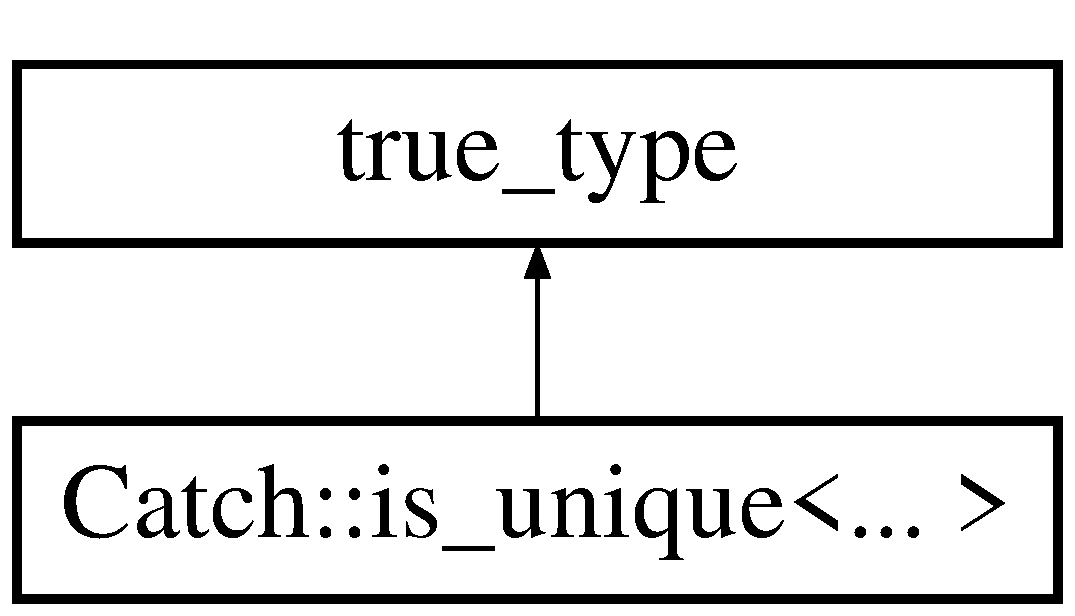
\includegraphics[height=2.000000cm]{struct_catch_1_1is__unique}
\end{center}
\end{figure}


The documentation for this struct was generated from the following file\+:\begin{DoxyCompactItemize}
\item 
D\+:/kouluhommat/\+Advanced Object-\/\+Oriented Programming/lopputyö/\+Battleship/\+Battleship/catch.\+hpp\end{DoxyCompactItemize}

\hypertarget{struct_catch_1_1is__unique_3_01_t0_00_01_t1_00_01_rest_8_8_8_01_4}{}\section{Catch\+:\+:is\+\_\+unique$<$ T0, T1, Rest... $>$ Struct Template Reference}
\label{struct_catch_1_1is__unique_3_01_t0_00_01_t1_00_01_rest_8_8_8_01_4}\index{Catch\+::is\+\_\+unique$<$ T0, T1, Rest... $>$@{Catch\+::is\+\_\+unique$<$ T0, T1, Rest... $>$}}
Inheritance diagram for Catch\+:\+:is\+\_\+unique$<$ T0, T1, Rest... $>$\+:\begin{figure}[H]
\begin{center}
\leavevmode
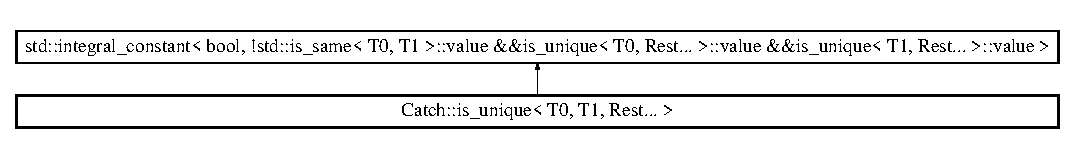
\includegraphics[height=1.483444cm]{struct_catch_1_1is__unique_3_01_t0_00_01_t1_00_01_rest_8_8_8_01_4}
\end{center}
\end{figure}


The documentation for this struct was generated from the following file\+:\begin{DoxyCompactItemize}
\item 
D\+:/kouluhommat/\+Advanced Object-\/\+Oriented Programming/lopputyö/\+Battleship/\+Battleship/catch.\+hpp\end{DoxyCompactItemize}

\hypertarget{class_catch_1_1_detail_1_1_is_stream_insertable}{}\section{Catch\+:\+:Detail\+:\+:Is\+Stream\+Insertable$<$ T $>$ Class Template Reference}
\label{class_catch_1_1_detail_1_1_is_stream_insertable}\index{Catch\+::\+Detail\+::\+Is\+Stream\+Insertable$<$ T $>$@{Catch\+::\+Detail\+::\+Is\+Stream\+Insertable$<$ T $>$}}
\subsection*{Static Public Attributes}
\begin{DoxyCompactItemize}
\item 
\mbox{\Hypertarget{class_catch_1_1_detail_1_1_is_stream_insertable_a42818b09ae5851126a70ee263769e309}\label{class_catch_1_1_detail_1_1_is_stream_insertable_a42818b09ae5851126a70ee263769e309}} 
static const bool {\bfseries value} = decltype(test$<$std\+::ostream, const T\&$>$(0))\+::value
\end{DoxyCompactItemize}


The documentation for this class was generated from the following file\+:\begin{DoxyCompactItemize}
\item 
D\+:/kouluhommat/\+Advanced Object-\/\+Oriented Programming/lopputyö/\+Battleship/\+Battleship/catch.\+hpp\end{DoxyCompactItemize}

\hypertarget{struct_catch_1_1_i_stream}{}\section{Catch\+:\+:I\+Stream Struct Reference}
\label{struct_catch_1_1_i_stream}\index{Catch\+::\+I\+Stream@{Catch\+::\+I\+Stream}}


{\ttfamily \#include $<$catch.\+hpp$>$}

\subsection*{Public Member Functions}
\begin{DoxyCompactItemize}
\item 
virtual \mbox{\hyperlink{struct_catch_1_1_i_stream_a344a88d0e5fc1f727f5801c72b4a4e2a}{$\sim$\+I\+Stream}} ()
\item 
virtual std\+::ostream \& \mbox{\hyperlink{struct_catch_1_1_i_stream_a55a9ddbe250261ff38642f480ebdd902}{stream}} () const =0
\end{DoxyCompactItemize}


\subsection{Constructor \& Destructor Documentation}
\mbox{\Hypertarget{struct_catch_1_1_i_stream_a344a88d0e5fc1f727f5801c72b4a4e2a}\label{struct_catch_1_1_i_stream_a344a88d0e5fc1f727f5801c72b4a4e2a}} 
\index{Catch\+::\+I\+Stream@{Catch\+::\+I\+Stream}!````~I\+Stream@{$\sim$\+I\+Stream}}
\index{````~I\+Stream@{$\sim$\+I\+Stream}!Catch\+::\+I\+Stream@{Catch\+::\+I\+Stream}}
\subsubsection{\texorpdfstring{$\sim$\+I\+Stream()}{~IStream()}}
{\footnotesize\ttfamily virtual Catch\+::\+I\+Stream\+::$\sim$\+I\+Stream (\begin{DoxyParamCaption}{ }\end{DoxyParamCaption})\hspace{0.3cm}{\ttfamily [virtual]}}



\subsection{Member Function Documentation}
\mbox{\Hypertarget{struct_catch_1_1_i_stream_a55a9ddbe250261ff38642f480ebdd902}\label{struct_catch_1_1_i_stream_a55a9ddbe250261ff38642f480ebdd902}} 
\index{Catch\+::\+I\+Stream@{Catch\+::\+I\+Stream}!stream@{stream}}
\index{stream@{stream}!Catch\+::\+I\+Stream@{Catch\+::\+I\+Stream}}
\subsubsection{\texorpdfstring{stream()}{stream()}}
{\footnotesize\ttfamily virtual std\+::ostream\& Catch\+::\+I\+Stream\+::stream (\begin{DoxyParamCaption}{ }\end{DoxyParamCaption}) const\hspace{0.3cm}{\ttfamily [pure virtual]}}



The documentation for this struct was generated from the following file\+:\begin{DoxyCompactItemize}
\item 
D\+:/kouluhommat/\+Advanced Object-\/\+Oriented Programming/lopputyö/\+Battleship/\+Battleship/\mbox{\hyperlink{catch_8hpp}{catch.\+hpp}}\end{DoxyCompactItemize}

\hypertarget{struct_catch_1_1_i_test_case_registry}{}\section{Catch\+:\+:I\+Test\+Case\+Registry Struct Reference}
\label{struct_catch_1_1_i_test_case_registry}\index{Catch\+::\+I\+Test\+Case\+Registry@{Catch\+::\+I\+Test\+Case\+Registry}}
\subsection*{Public Member Functions}
\begin{DoxyCompactItemize}
\item 
\mbox{\Hypertarget{struct_catch_1_1_i_test_case_registry_ad6e4d4a621655123f73ae98cfeda063d}\label{struct_catch_1_1_i_test_case_registry_ad6e4d4a621655123f73ae98cfeda063d}} 
virtual std\+::vector$<$ \mbox{\hyperlink{class_catch_1_1_test_case}{Test\+Case}} $>$ const  \& {\bfseries get\+All\+Tests} () const =0
\item 
\mbox{\Hypertarget{struct_catch_1_1_i_test_case_registry_a33e46639d0319d35497c05bb5d02be5a}\label{struct_catch_1_1_i_test_case_registry_a33e46639d0319d35497c05bb5d02be5a}} 
virtual std\+::vector$<$ \mbox{\hyperlink{class_catch_1_1_test_case}{Test\+Case}} $>$ const  \& {\bfseries get\+All\+Tests\+Sorted} (I\+Config const \&config) const =0
\end{DoxyCompactItemize}


The documentation for this struct was generated from the following file\+:\begin{DoxyCompactItemize}
\item 
D\+:/kouluhommat/\+Advanced Object-\/\+Oriented Programming/lopputyö/\+Battleship/\+Battleship/catch.\+hpp\end{DoxyCompactItemize}

\hypertarget{struct_catch_1_1_i_test_invoker}{}\section{Catch\+:\+:I\+Test\+Invoker Struct Reference}
\label{struct_catch_1_1_i_test_invoker}\index{Catch\+::\+I\+Test\+Invoker@{Catch\+::\+I\+Test\+Invoker}}
Inheritance diagram for Catch\+:\+:I\+Test\+Invoker\+:\begin{figure}[H]
\begin{center}
\leavevmode
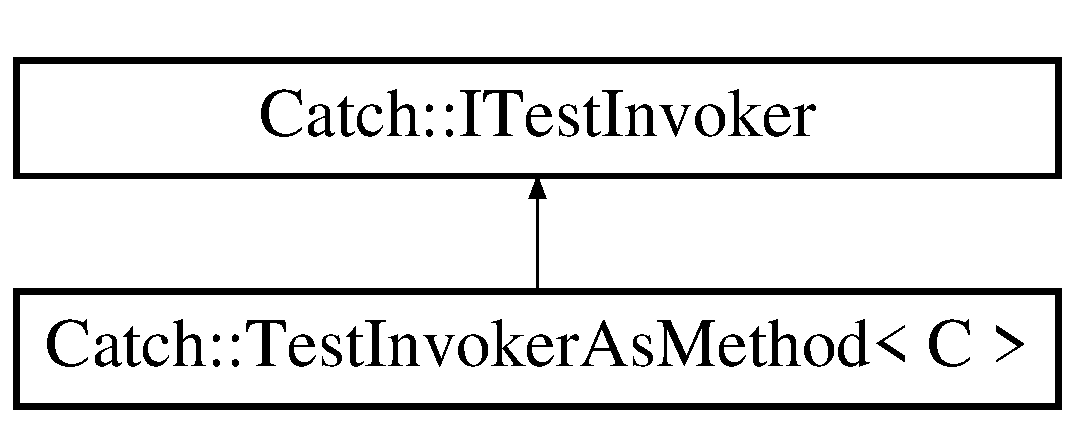
\includegraphics[height=2.000000cm]{struct_catch_1_1_i_test_invoker}
\end{center}
\end{figure}
\subsection*{Public Member Functions}
\begin{DoxyCompactItemize}
\item 
\mbox{\Hypertarget{struct_catch_1_1_i_test_invoker_a6fcd5c5b67d6d5ade6491ff33411ca7f}\label{struct_catch_1_1_i_test_invoker_a6fcd5c5b67d6d5ade6491ff33411ca7f}} 
virtual void {\bfseries invoke} () const =0
\end{DoxyCompactItemize}


The documentation for this struct was generated from the following file\+:\begin{DoxyCompactItemize}
\item 
D\+:/kouluhommat/\+Advanced Object-\/\+Oriented Programming/lopputyö/\+Battleship/\+Battleship/catch.\+hpp\end{DoxyCompactItemize}

\hypertarget{struct_catch_1_1_i_transient_expression}{}\section{Catch\+:\+:I\+Transient\+Expression Struct Reference}
\label{struct_catch_1_1_i_transient_expression}\index{Catch\+::\+I\+Transient\+Expression@{Catch\+::\+I\+Transient\+Expression}}


{\ttfamily \#include $<$catch.\+hpp$>$}

Inheritance diagram for Catch\+:\+:I\+Transient\+Expression\+:\begin{figure}[H]
\begin{center}
\leavevmode
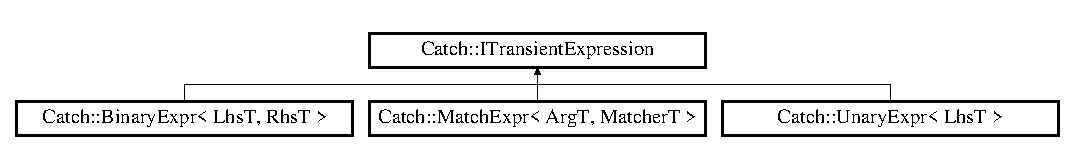
\includegraphics[height=1.588652cm]{struct_catch_1_1_i_transient_expression}
\end{center}
\end{figure}
\subsection*{Public Member Functions}
\begin{DoxyCompactItemize}
\item 
auto \mbox{\hyperlink{struct_catch_1_1_i_transient_expression_a3b436e13a0a6d3522bbf70d4e31deb22}{is\+Binary\+Expression}} () const -\/$>$ bool
\item 
auto \mbox{\hyperlink{struct_catch_1_1_i_transient_expression_a101c7db86c87eff93a8ff496720e6320}{get\+Result}} () const -\/$>$ bool
\item 
virtual void \mbox{\hyperlink{struct_catch_1_1_i_transient_expression_aabe1889df9c6e639a24afb08d8a0fe9e}{stream\+Reconstructed\+Expression}} (std\+::ostream \&os) const =0
\item 
\mbox{\hyperlink{struct_catch_1_1_i_transient_expression_aafe69572b7ed884e63ec81f58d4afd8c}{I\+Transient\+Expression}} (bool \mbox{\hyperlink{struct_catch_1_1_i_transient_expression_a3b436e13a0a6d3522bbf70d4e31deb22}{is\+Binary\+Expression}}, bool result)
\item 
virtual \mbox{\hyperlink{struct_catch_1_1_i_transient_expression_aeadf426de589938c4964fe4068eeee77}{$\sim$\+I\+Transient\+Expression}} ()
\end{DoxyCompactItemize}
\subsection*{Public Attributes}
\begin{DoxyCompactItemize}
\item 
bool \mbox{\hyperlink{struct_catch_1_1_i_transient_expression_a75ce48da824d514d08152d396abb28d8}{m\+\_\+is\+Binary\+Expression}}
\item 
bool \mbox{\hyperlink{struct_catch_1_1_i_transient_expression_a4646e2b5e0156e913653ec3b9b60c942}{m\+\_\+result}}
\end{DoxyCompactItemize}


\subsection{Constructor \& Destructor Documentation}
\mbox{\Hypertarget{struct_catch_1_1_i_transient_expression_aafe69572b7ed884e63ec81f58d4afd8c}\label{struct_catch_1_1_i_transient_expression_aafe69572b7ed884e63ec81f58d4afd8c}} 
\index{Catch\+::\+I\+Transient\+Expression@{Catch\+::\+I\+Transient\+Expression}!I\+Transient\+Expression@{I\+Transient\+Expression}}
\index{I\+Transient\+Expression@{I\+Transient\+Expression}!Catch\+::\+I\+Transient\+Expression@{Catch\+::\+I\+Transient\+Expression}}
\subsubsection{\texorpdfstring{I\+Transient\+Expression()}{ITransientExpression()}}
{\footnotesize\ttfamily Catch\+::\+I\+Transient\+Expression\+::\+I\+Transient\+Expression (\begin{DoxyParamCaption}\item[{bool}]{is\+Binary\+Expression,  }\item[{bool}]{result }\end{DoxyParamCaption})\hspace{0.3cm}{\ttfamily [inline]}}

\mbox{\Hypertarget{struct_catch_1_1_i_transient_expression_aeadf426de589938c4964fe4068eeee77}\label{struct_catch_1_1_i_transient_expression_aeadf426de589938c4964fe4068eeee77}} 
\index{Catch\+::\+I\+Transient\+Expression@{Catch\+::\+I\+Transient\+Expression}!````~I\+Transient\+Expression@{$\sim$\+I\+Transient\+Expression}}
\index{````~I\+Transient\+Expression@{$\sim$\+I\+Transient\+Expression}!Catch\+::\+I\+Transient\+Expression@{Catch\+::\+I\+Transient\+Expression}}
\subsubsection{\texorpdfstring{$\sim$\+I\+Transient\+Expression()}{~ITransientExpression()}}
{\footnotesize\ttfamily virtual Catch\+::\+I\+Transient\+Expression\+::$\sim$\+I\+Transient\+Expression (\begin{DoxyParamCaption}{ }\end{DoxyParamCaption})\hspace{0.3cm}{\ttfamily [virtual]}}



\subsection{Member Function Documentation}
\mbox{\Hypertarget{struct_catch_1_1_i_transient_expression_a101c7db86c87eff93a8ff496720e6320}\label{struct_catch_1_1_i_transient_expression_a101c7db86c87eff93a8ff496720e6320}} 
\index{Catch\+::\+I\+Transient\+Expression@{Catch\+::\+I\+Transient\+Expression}!get\+Result@{get\+Result}}
\index{get\+Result@{get\+Result}!Catch\+::\+I\+Transient\+Expression@{Catch\+::\+I\+Transient\+Expression}}
\subsubsection{\texorpdfstring{get\+Result()}{getResult()}}
{\footnotesize\ttfamily auto Catch\+::\+I\+Transient\+Expression\+::get\+Result (\begin{DoxyParamCaption}{ }\end{DoxyParamCaption}) const -\/$>$ bool \hspace{0.3cm}{\ttfamily [inline]}}

\mbox{\Hypertarget{struct_catch_1_1_i_transient_expression_a3b436e13a0a6d3522bbf70d4e31deb22}\label{struct_catch_1_1_i_transient_expression_a3b436e13a0a6d3522bbf70d4e31deb22}} 
\index{Catch\+::\+I\+Transient\+Expression@{Catch\+::\+I\+Transient\+Expression}!is\+Binary\+Expression@{is\+Binary\+Expression}}
\index{is\+Binary\+Expression@{is\+Binary\+Expression}!Catch\+::\+I\+Transient\+Expression@{Catch\+::\+I\+Transient\+Expression}}
\subsubsection{\texorpdfstring{is\+Binary\+Expression()}{isBinaryExpression()}}
{\footnotesize\ttfamily auto Catch\+::\+I\+Transient\+Expression\+::is\+Binary\+Expression (\begin{DoxyParamCaption}{ }\end{DoxyParamCaption}) const -\/$>$ bool \hspace{0.3cm}{\ttfamily [inline]}}

\mbox{\Hypertarget{struct_catch_1_1_i_transient_expression_aabe1889df9c6e639a24afb08d8a0fe9e}\label{struct_catch_1_1_i_transient_expression_aabe1889df9c6e639a24afb08d8a0fe9e}} 
\index{Catch\+::\+I\+Transient\+Expression@{Catch\+::\+I\+Transient\+Expression}!stream\+Reconstructed\+Expression@{stream\+Reconstructed\+Expression}}
\index{stream\+Reconstructed\+Expression@{stream\+Reconstructed\+Expression}!Catch\+::\+I\+Transient\+Expression@{Catch\+::\+I\+Transient\+Expression}}
\subsubsection{\texorpdfstring{stream\+Reconstructed\+Expression()}{streamReconstructedExpression()}}
{\footnotesize\ttfamily virtual void Catch\+::\+I\+Transient\+Expression\+::stream\+Reconstructed\+Expression (\begin{DoxyParamCaption}\item[{std\+::ostream \&}]{os }\end{DoxyParamCaption}) const\hspace{0.3cm}{\ttfamily [pure virtual]}}



Implemented in \mbox{\hyperlink{class_catch_1_1_match_expr_ad3e41adb597750b2219bb37e51185629}{Catch\+::\+Match\+Expr$<$ Arg\+T, Matcher\+T $>$}}.



\subsection{Member Data Documentation}
\mbox{\Hypertarget{struct_catch_1_1_i_transient_expression_a75ce48da824d514d08152d396abb28d8}\label{struct_catch_1_1_i_transient_expression_a75ce48da824d514d08152d396abb28d8}} 
\index{Catch\+::\+I\+Transient\+Expression@{Catch\+::\+I\+Transient\+Expression}!m\+\_\+is\+Binary\+Expression@{m\+\_\+is\+Binary\+Expression}}
\index{m\+\_\+is\+Binary\+Expression@{m\+\_\+is\+Binary\+Expression}!Catch\+::\+I\+Transient\+Expression@{Catch\+::\+I\+Transient\+Expression}}
\subsubsection{\texorpdfstring{m\+\_\+is\+Binary\+Expression}{m\_isBinaryExpression}}
{\footnotesize\ttfamily bool Catch\+::\+I\+Transient\+Expression\+::m\+\_\+is\+Binary\+Expression}

\mbox{\Hypertarget{struct_catch_1_1_i_transient_expression_a4646e2b5e0156e913653ec3b9b60c942}\label{struct_catch_1_1_i_transient_expression_a4646e2b5e0156e913653ec3b9b60c942}} 
\index{Catch\+::\+I\+Transient\+Expression@{Catch\+::\+I\+Transient\+Expression}!m\+\_\+result@{m\+\_\+result}}
\index{m\+\_\+result@{m\+\_\+result}!Catch\+::\+I\+Transient\+Expression@{Catch\+::\+I\+Transient\+Expression}}
\subsubsection{\texorpdfstring{m\+\_\+result}{m\_result}}
{\footnotesize\ttfamily bool Catch\+::\+I\+Transient\+Expression\+::m\+\_\+result}



The documentation for this struct was generated from the following file\+:\begin{DoxyCompactItemize}
\item 
D\+:/kouluhommat/\+Advanced Object-\/\+Oriented Programming/lopputyö/\+Battleship/\+Battleship/\mbox{\hyperlink{catch_8hpp}{catch.\+hpp}}\end{DoxyCompactItemize}

\hypertarget{class_catch_1_1_lazy_expression}{}\section{Catch\+:\+:Lazy\+Expression Class Reference}
\label{class_catch_1_1_lazy_expression}\index{Catch\+::\+Lazy\+Expression@{Catch\+::\+Lazy\+Expression}}
\subsection*{Public Member Functions}
\begin{DoxyCompactItemize}
\item 
\mbox{\Hypertarget{class_catch_1_1_lazy_expression_a47186c2487bd4bf871e870ba8048553a}\label{class_catch_1_1_lazy_expression_a47186c2487bd4bf871e870ba8048553a}} 
{\bfseries Lazy\+Expression} (bool is\+Negated)
\item 
\mbox{\Hypertarget{class_catch_1_1_lazy_expression_ab82d5e94df0e159b018fbde0170e46f8}\label{class_catch_1_1_lazy_expression_ab82d5e94df0e159b018fbde0170e46f8}} 
{\bfseries Lazy\+Expression} (\mbox{\hyperlink{class_catch_1_1_lazy_expression}{Lazy\+Expression}} const \&other)
\item 
\mbox{\Hypertarget{class_catch_1_1_lazy_expression_ae4ae00d4f36f084c369f2da36565a822}\label{class_catch_1_1_lazy_expression_ae4ae00d4f36f084c369f2da36565a822}} 
\mbox{\hyperlink{class_catch_1_1_lazy_expression}{Lazy\+Expression}} \& {\bfseries operator=} (\mbox{\hyperlink{class_catch_1_1_lazy_expression}{Lazy\+Expression}} const \&)=delete
\item 
\mbox{\Hypertarget{class_catch_1_1_lazy_expression_acdb846cb230cecfc6aca7a925b31fbca}\label{class_catch_1_1_lazy_expression_acdb846cb230cecfc6aca7a925b31fbca}} 
{\bfseries operator bool} () const
\end{DoxyCompactItemize}
\subsection*{Friends}
\begin{DoxyCompactItemize}
\item 
\mbox{\Hypertarget{class_catch_1_1_lazy_expression_a4301a3aa57b612dd8b6ef8461742ecab}\label{class_catch_1_1_lazy_expression_a4301a3aa57b612dd8b6ef8461742ecab}} 
class {\bfseries Assertion\+Handler}
\item 
\mbox{\Hypertarget{class_catch_1_1_lazy_expression_a64019eb137f5ce447cdc71cb80b6e7a4}\label{class_catch_1_1_lazy_expression_a64019eb137f5ce447cdc71cb80b6e7a4}} 
struct {\bfseries Assertion\+Stats}
\item 
\mbox{\Hypertarget{class_catch_1_1_lazy_expression_af3aa096bb29a772bc534830f29a2ce7a}\label{class_catch_1_1_lazy_expression_af3aa096bb29a772bc534830f29a2ce7a}} 
class {\bfseries Run\+Context}
\item 
\mbox{\Hypertarget{class_catch_1_1_lazy_expression_aa01086581cab2fcd2d4580b8fa787dfc}\label{class_catch_1_1_lazy_expression_aa01086581cab2fcd2d4580b8fa787dfc}} 
auto {\bfseries operator$<$$<$} (std\+::ostream \&os, \mbox{\hyperlink{class_catch_1_1_lazy_expression}{Lazy\+Expression}} const \&lazy\+Expr) -\/$>$ std\+::ostream \&
\end{DoxyCompactItemize}


The documentation for this class was generated from the following file\+:\begin{DoxyCompactItemize}
\item 
D\+:/kouluhommat/\+Advanced Object-\/\+Oriented Programming/lopputyö/\+Battleship/\+Battleship/catch.\+hpp\end{DoxyCompactItemize}

\hypertarget{struct_catch_1_1_matchers_1_1_impl_1_1_match_all_of}{}\section{Catch\+:\+:Matchers\+:\+:Impl\+:\+:Match\+All\+Of$<$ ArgT $>$ Struct Template Reference}
\label{struct_catch_1_1_matchers_1_1_impl_1_1_match_all_of}\index{Catch\+::\+Matchers\+::\+Impl\+::\+Match\+All\+Of$<$ Arg\+T $>$@{Catch\+::\+Matchers\+::\+Impl\+::\+Match\+All\+Of$<$ Arg\+T $>$}}
Inheritance diagram for Catch\+:\+:Matchers\+:\+:Impl\+:\+:Match\+All\+Of$<$ ArgT $>$\+:\begin{figure}[H]
\begin{center}
\leavevmode
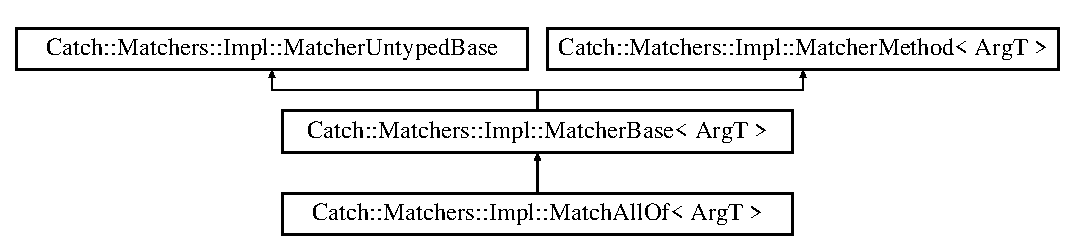
\includegraphics[height=2.926829cm]{struct_catch_1_1_matchers_1_1_impl_1_1_match_all_of}
\end{center}
\end{figure}
\subsection*{Public Member Functions}
\begin{DoxyCompactItemize}
\item 
\mbox{\Hypertarget{struct_catch_1_1_matchers_1_1_impl_1_1_match_all_of_acfb377bda2c58ae62e6df9c3a8a89f8f}\label{struct_catch_1_1_matchers_1_1_impl_1_1_match_all_of_acfb377bda2c58ae62e6df9c3a8a89f8f}} 
bool {\bfseries match} (ArgT const \&arg) const override
\item 
\mbox{\Hypertarget{struct_catch_1_1_matchers_1_1_impl_1_1_match_all_of_acbb9a083e93b546fd33c9235b644c40f}\label{struct_catch_1_1_matchers_1_1_impl_1_1_match_all_of_acbb9a083e93b546fd33c9235b644c40f}} 
std\+::string {\bfseries describe} () const override
\item 
\mbox{\Hypertarget{struct_catch_1_1_matchers_1_1_impl_1_1_match_all_of_a9d0e38b36474336498d627610db434f3}\label{struct_catch_1_1_matchers_1_1_impl_1_1_match_all_of_a9d0e38b36474336498d627610db434f3}} 
\mbox{\hyperlink{struct_catch_1_1_matchers_1_1_impl_1_1_match_all_of}{Match\+All\+Of}}$<$ ArgT $>$ \& {\bfseries operator\&\&} (\mbox{\hyperlink{struct_catch_1_1_matchers_1_1_impl_1_1_matcher_base}{Matcher\+Base}}$<$ ArgT $>$ const \&other)
\end{DoxyCompactItemize}
\subsection*{Public Attributes}
\begin{DoxyCompactItemize}
\item 
\mbox{\Hypertarget{struct_catch_1_1_matchers_1_1_impl_1_1_match_all_of_a98d6a2611f195a4a5c49f92fd877be9a}\label{struct_catch_1_1_matchers_1_1_impl_1_1_match_all_of_a98d6a2611f195a4a5c49f92fd877be9a}} 
std\+::vector$<$ \mbox{\hyperlink{struct_catch_1_1_matchers_1_1_impl_1_1_matcher_base}{Matcher\+Base}}$<$ ArgT $>$ const  $\ast$ $>$ {\bfseries m\+\_\+matchers}
\end{DoxyCompactItemize}
\subsection*{Additional Inherited Members}


The documentation for this struct was generated from the following file\+:\begin{DoxyCompactItemize}
\item 
D\+:/kouluhommat/\+Advanced Object-\/\+Oriented Programming/lopputyö/\+Battleship/\+Battleship/catch.\+hpp\end{DoxyCompactItemize}

\hypertarget{struct_catch_1_1_matchers_1_1_impl_1_1_match_any_of}{}\section{Catch\+:\+:Matchers\+:\+:Impl\+:\+:Match\+Any\+Of$<$ ArgT $>$ Struct Template Reference}
\label{struct_catch_1_1_matchers_1_1_impl_1_1_match_any_of}\index{Catch\+::\+Matchers\+::\+Impl\+::\+Match\+Any\+Of$<$ Arg\+T $>$@{Catch\+::\+Matchers\+::\+Impl\+::\+Match\+Any\+Of$<$ Arg\+T $>$}}
Inheritance diagram for Catch\+:\+:Matchers\+:\+:Impl\+:\+:Match\+Any\+Of$<$ ArgT $>$\+:\begin{figure}[H]
\begin{center}
\leavevmode
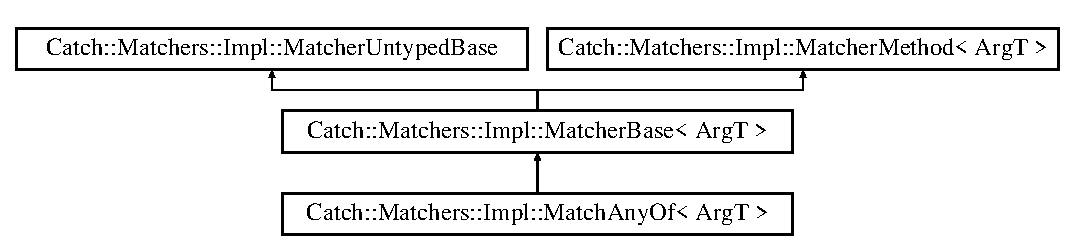
\includegraphics[height=2.926829cm]{struct_catch_1_1_matchers_1_1_impl_1_1_match_any_of}
\end{center}
\end{figure}
\subsection*{Public Member Functions}
\begin{DoxyCompactItemize}
\item 
\mbox{\Hypertarget{struct_catch_1_1_matchers_1_1_impl_1_1_match_any_of_a8a3e8338f979e56277dcf553efb78dc0}\label{struct_catch_1_1_matchers_1_1_impl_1_1_match_any_of_a8a3e8338f979e56277dcf553efb78dc0}} 
bool {\bfseries match} (ArgT const \&arg) const override
\item 
\mbox{\Hypertarget{struct_catch_1_1_matchers_1_1_impl_1_1_match_any_of_a315285204df93d1f8e72f50dd66eb709}\label{struct_catch_1_1_matchers_1_1_impl_1_1_match_any_of_a315285204df93d1f8e72f50dd66eb709}} 
std\+::string {\bfseries describe} () const override
\item 
\mbox{\Hypertarget{struct_catch_1_1_matchers_1_1_impl_1_1_match_any_of_a44d7582dbe09fc31b9a5ba8a6367b506}\label{struct_catch_1_1_matchers_1_1_impl_1_1_match_any_of_a44d7582dbe09fc31b9a5ba8a6367b506}} 
\mbox{\hyperlink{struct_catch_1_1_matchers_1_1_impl_1_1_match_any_of}{Match\+Any\+Of}}$<$ ArgT $>$ \& {\bfseries operator$\vert$$\vert$} (\mbox{\hyperlink{struct_catch_1_1_matchers_1_1_impl_1_1_matcher_base}{Matcher\+Base}}$<$ ArgT $>$ const \&other)
\end{DoxyCompactItemize}
\subsection*{Public Attributes}
\begin{DoxyCompactItemize}
\item 
\mbox{\Hypertarget{struct_catch_1_1_matchers_1_1_impl_1_1_match_any_of_a1fb1119e6110dc15b8d5262ec0aeddd5}\label{struct_catch_1_1_matchers_1_1_impl_1_1_match_any_of_a1fb1119e6110dc15b8d5262ec0aeddd5}} 
std\+::vector$<$ \mbox{\hyperlink{struct_catch_1_1_matchers_1_1_impl_1_1_matcher_base}{Matcher\+Base}}$<$ ArgT $>$ const  $\ast$ $>$ {\bfseries m\+\_\+matchers}
\end{DoxyCompactItemize}
\subsection*{Additional Inherited Members}


The documentation for this struct was generated from the following file\+:\begin{DoxyCompactItemize}
\item 
D\+:/kouluhommat/\+Advanced Object-\/\+Oriented Programming/lopputyö/\+Battleship/\+Battleship/catch.\+hpp\end{DoxyCompactItemize}

\hypertarget{struct_catch_1_1_matchers_1_1_impl_1_1_matcher_base}{}\section{Catch\+:\+:Matchers\+:\+:Impl\+:\+:Matcher\+Base$<$ T $>$ Struct Template Reference}
\label{struct_catch_1_1_matchers_1_1_impl_1_1_matcher_base}\index{Catch\+::\+Matchers\+::\+Impl\+::\+Matcher\+Base$<$ T $>$@{Catch\+::\+Matchers\+::\+Impl\+::\+Matcher\+Base$<$ T $>$}}


{\ttfamily \#include $<$catch.\+hpp$>$}

Inheritance diagram for Catch\+:\+:Matchers\+:\+:Impl\+:\+:Matcher\+Base$<$ T $>$\+:\begin{figure}[H]
\begin{center}
\leavevmode
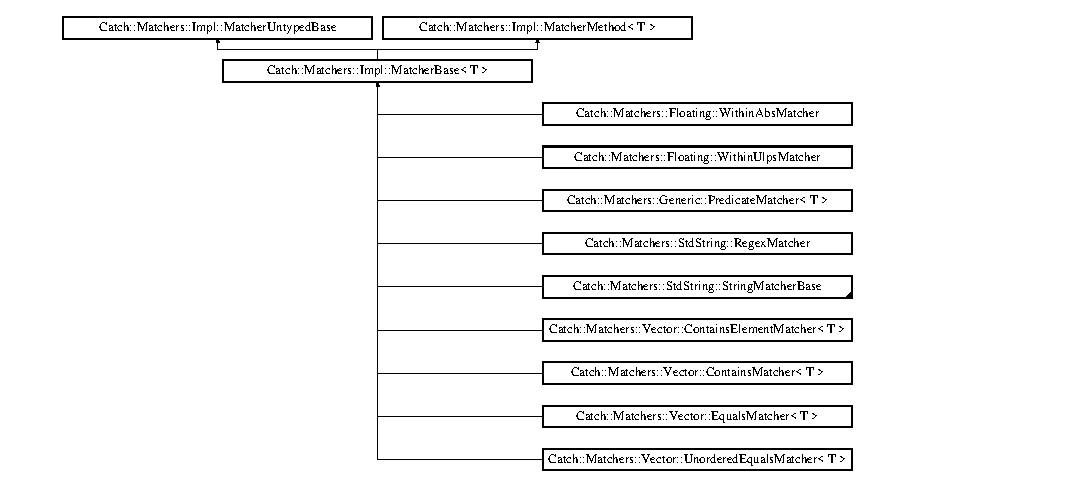
\includegraphics[height=6.092978cm]{struct_catch_1_1_matchers_1_1_impl_1_1_matcher_base}
\end{center}
\end{figure}
\subsection*{Public Member Functions}
\begin{DoxyCompactItemize}
\item 
\mbox{\hyperlink{struct_catch_1_1_matchers_1_1_impl_1_1_match_all_of}{Match\+All\+Of}}$<$ T $>$ \mbox{\hyperlink{struct_catch_1_1_matchers_1_1_impl_1_1_matcher_base_a23c336f6d9457735ddc8dc7ea864d7c9}{operator\&\&}} (\mbox{\hyperlink{struct_catch_1_1_matchers_1_1_impl_1_1_matcher_base}{Matcher\+Base}} const \&other) const
\item 
\mbox{\hyperlink{struct_catch_1_1_matchers_1_1_impl_1_1_match_any_of}{Match\+Any\+Of}}$<$ T $>$ \mbox{\hyperlink{struct_catch_1_1_matchers_1_1_impl_1_1_matcher_base_a5f8542b8f1567a6f9c65d0a6da7b679b}{operator$\vert$$\vert$}} (\mbox{\hyperlink{struct_catch_1_1_matchers_1_1_impl_1_1_matcher_base}{Matcher\+Base}} const \&other) const
\item 
\mbox{\hyperlink{struct_catch_1_1_matchers_1_1_impl_1_1_match_not_of}{Match\+Not\+Of}}$<$ T $>$ \mbox{\hyperlink{struct_catch_1_1_matchers_1_1_impl_1_1_matcher_base_a5bb94bf2ff5c7ef73b7c11eb173bdf3b}{operator!}} () const
\end{DoxyCompactItemize}
\subsection*{Additional Inherited Members}


\subsection{Member Function Documentation}
\mbox{\Hypertarget{struct_catch_1_1_matchers_1_1_impl_1_1_matcher_base_a5bb94bf2ff5c7ef73b7c11eb173bdf3b}\label{struct_catch_1_1_matchers_1_1_impl_1_1_matcher_base_a5bb94bf2ff5c7ef73b7c11eb173bdf3b}} 
\index{Catch\+::\+Matchers\+::\+Impl\+::\+Matcher\+Base@{Catch\+::\+Matchers\+::\+Impl\+::\+Matcher\+Base}!operator"!@{operator"!}}
\index{operator"!@{operator"!}!Catch\+::\+Matchers\+::\+Impl\+::\+Matcher\+Base@{Catch\+::\+Matchers\+::\+Impl\+::\+Matcher\+Base}}
\subsubsection{\texorpdfstring{operator"!()}{operator!()}}
{\footnotesize\ttfamily template$<$typename T $>$ \\
\mbox{\hyperlink{struct_catch_1_1_matchers_1_1_impl_1_1_match_not_of}{Match\+Not\+Of}}$<$ T $>$ \mbox{\hyperlink{struct_catch_1_1_matchers_1_1_impl_1_1_matcher_base}{Catch\+::\+Matchers\+::\+Impl\+::\+Matcher\+Base}}$<$ T $>$\+::operator! (\begin{DoxyParamCaption}{ }\end{DoxyParamCaption}) const}

\mbox{\Hypertarget{struct_catch_1_1_matchers_1_1_impl_1_1_matcher_base_a23c336f6d9457735ddc8dc7ea864d7c9}\label{struct_catch_1_1_matchers_1_1_impl_1_1_matcher_base_a23c336f6d9457735ddc8dc7ea864d7c9}} 
\index{Catch\+::\+Matchers\+::\+Impl\+::\+Matcher\+Base@{Catch\+::\+Matchers\+::\+Impl\+::\+Matcher\+Base}!operator\&\&@{operator\&\&}}
\index{operator\&\&@{operator\&\&}!Catch\+::\+Matchers\+::\+Impl\+::\+Matcher\+Base@{Catch\+::\+Matchers\+::\+Impl\+::\+Matcher\+Base}}
\subsubsection{\texorpdfstring{operator\&\&()}{operator\&\&()}}
{\footnotesize\ttfamily template$<$typename T$>$ \\
\mbox{\hyperlink{struct_catch_1_1_matchers_1_1_impl_1_1_match_all_of}{Match\+All\+Of}}$<$T$>$ \mbox{\hyperlink{struct_catch_1_1_matchers_1_1_impl_1_1_matcher_base}{Catch\+::\+Matchers\+::\+Impl\+::\+Matcher\+Base}}$<$ T $>$\+::operator \&\& (\begin{DoxyParamCaption}\item[{\mbox{\hyperlink{struct_catch_1_1_matchers_1_1_impl_1_1_matcher_base}{Matcher\+Base}}$<$ T $>$ const \&}]{other }\end{DoxyParamCaption}) const}

\mbox{\Hypertarget{struct_catch_1_1_matchers_1_1_impl_1_1_matcher_base_a5f8542b8f1567a6f9c65d0a6da7b679b}\label{struct_catch_1_1_matchers_1_1_impl_1_1_matcher_base_a5f8542b8f1567a6f9c65d0a6da7b679b}} 
\index{Catch\+::\+Matchers\+::\+Impl\+::\+Matcher\+Base@{Catch\+::\+Matchers\+::\+Impl\+::\+Matcher\+Base}!operator\texttt{"|}\texttt{"|}@{operator\texttt{"|}\texttt{"|}}}
\index{operator\texttt{"|}\texttt{"|}@{operator\texttt{"|}\texttt{"|}}!Catch\+::\+Matchers\+::\+Impl\+::\+Matcher\+Base@{Catch\+::\+Matchers\+::\+Impl\+::\+Matcher\+Base}}
\subsubsection{\texorpdfstring{operator\texttt{"|}\texttt{"|}()}{operator||()}}
{\footnotesize\ttfamily template$<$typename T $>$ \\
\mbox{\hyperlink{struct_catch_1_1_matchers_1_1_impl_1_1_match_any_of}{Match\+Any\+Of}}$<$ T $>$ \mbox{\hyperlink{struct_catch_1_1_matchers_1_1_impl_1_1_matcher_base}{Catch\+::\+Matchers\+::\+Impl\+::\+Matcher\+Base}}$<$ T $>$\+::operator$\vert$$\vert$ (\begin{DoxyParamCaption}\item[{\mbox{\hyperlink{struct_catch_1_1_matchers_1_1_impl_1_1_matcher_base}{Matcher\+Base}}$<$ T $>$ const \&}]{other }\end{DoxyParamCaption}) const}



The documentation for this struct was generated from the following file\+:\begin{DoxyCompactItemize}
\item 
D\+:/kouluhommat/\+Advanced Object-\/\+Oriented Programming/lopputyö/\+Battleship/\+Battleship/\mbox{\hyperlink{catch_8hpp}{catch.\+hpp}}\end{DoxyCompactItemize}

\hypertarget{struct_catch_1_1_matchers_1_1_impl_1_1_matcher_method}{}\section{Catch\+:\+:Matchers\+:\+:Impl\+:\+:Matcher\+Method$<$ ObjectT $>$ Struct Template Reference}
\label{struct_catch_1_1_matchers_1_1_impl_1_1_matcher_method}\index{Catch\+::\+Matchers\+::\+Impl\+::\+Matcher\+Method$<$ Object\+T $>$@{Catch\+::\+Matchers\+::\+Impl\+::\+Matcher\+Method$<$ Object\+T $>$}}
\subsection*{Public Member Functions}
\begin{DoxyCompactItemize}
\item 
\mbox{\Hypertarget{struct_catch_1_1_matchers_1_1_impl_1_1_matcher_method_ae0920ff9e817acf08e1bb0cbcb044e30}\label{struct_catch_1_1_matchers_1_1_impl_1_1_matcher_method_ae0920ff9e817acf08e1bb0cbcb044e30}} 
virtual bool {\bfseries match} (ObjectT const \&arg) const =0
\end{DoxyCompactItemize}


The documentation for this struct was generated from the following file\+:\begin{DoxyCompactItemize}
\item 
D\+:/kouluhommat/\+Advanced Object-\/\+Oriented Programming/lopputyö/\+Battleship/\+Battleship/catch.\+hpp\end{DoxyCompactItemize}

\hypertarget{class_catch_1_1_matchers_1_1_impl_1_1_matcher_untyped_base}{}\section{Catch\+:\+:Matchers\+:\+:Impl\+:\+:Matcher\+Untyped\+Base Class Reference}
\label{class_catch_1_1_matchers_1_1_impl_1_1_matcher_untyped_base}\index{Catch\+::\+Matchers\+::\+Impl\+::\+Matcher\+Untyped\+Base@{Catch\+::\+Matchers\+::\+Impl\+::\+Matcher\+Untyped\+Base}}


{\ttfamily \#include $<$catch.\+hpp$>$}

Inheritance diagram for Catch\+:\+:Matchers\+:\+:Impl\+:\+:Matcher\+Untyped\+Base\+:\begin{figure}[H]
\begin{center}
\leavevmode
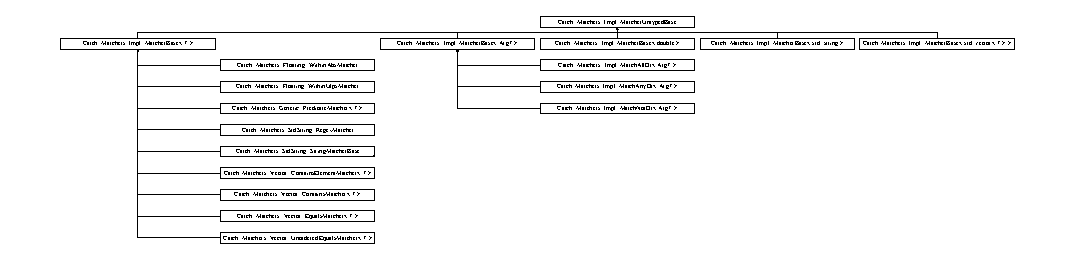
\includegraphics[height=3.046489cm]{class_catch_1_1_matchers_1_1_impl_1_1_matcher_untyped_base}
\end{center}
\end{figure}
\subsection*{Public Member Functions}
\begin{DoxyCompactItemize}
\item 
\mbox{\hyperlink{class_catch_1_1_matchers_1_1_impl_1_1_matcher_untyped_base_ab65764dc245d85e2b268d3be870b650a}{Matcher\+Untyped\+Base}} ()=default
\item 
\mbox{\hyperlink{class_catch_1_1_matchers_1_1_impl_1_1_matcher_untyped_base_a985fd3c3ffcc9f2e8dc7a330130040b0}{Matcher\+Untyped\+Base}} (\mbox{\hyperlink{class_catch_1_1_matchers_1_1_impl_1_1_matcher_untyped_base}{Matcher\+Untyped\+Base}} const \&)=default
\item 
\mbox{\hyperlink{class_catch_1_1_matchers_1_1_impl_1_1_matcher_untyped_base}{Matcher\+Untyped\+Base}} \& \mbox{\hyperlink{class_catch_1_1_matchers_1_1_impl_1_1_matcher_untyped_base_a62668ccc47b64a9094dcb6413f9af80b}{operator=}} (\mbox{\hyperlink{class_catch_1_1_matchers_1_1_impl_1_1_matcher_untyped_base}{Matcher\+Untyped\+Base}} const \&)=delete
\item 
std\+::string \mbox{\hyperlink{class_catch_1_1_matchers_1_1_impl_1_1_matcher_untyped_base_a5982c7c80ca71dfe2298babadad7a453}{to\+String}} () const
\end{DoxyCompactItemize}
\subsection*{Protected Member Functions}
\begin{DoxyCompactItemize}
\item 
virtual \mbox{\hyperlink{class_catch_1_1_matchers_1_1_impl_1_1_matcher_untyped_base_a853be93ce33f71b5abede38081c79e9d}{$\sim$\+Matcher\+Untyped\+Base}} ()
\item 
virtual std\+::string \mbox{\hyperlink{class_catch_1_1_matchers_1_1_impl_1_1_matcher_untyped_base_a91d3a907dbfcbb596077df24f6e11fe2}{describe}} () const =0
\end{DoxyCompactItemize}
\subsection*{Protected Attributes}
\begin{DoxyCompactItemize}
\item 
std\+::string \mbox{\hyperlink{class_catch_1_1_matchers_1_1_impl_1_1_matcher_untyped_base_a951095c462657e7097a9a6dc4dde813f}{m\+\_\+cached\+To\+String}}
\end{DoxyCompactItemize}


\subsection{Constructor \& Destructor Documentation}
\mbox{\Hypertarget{class_catch_1_1_matchers_1_1_impl_1_1_matcher_untyped_base_ab65764dc245d85e2b268d3be870b650a}\label{class_catch_1_1_matchers_1_1_impl_1_1_matcher_untyped_base_ab65764dc245d85e2b268d3be870b650a}} 
\index{Catch\+::\+Matchers\+::\+Impl\+::\+Matcher\+Untyped\+Base@{Catch\+::\+Matchers\+::\+Impl\+::\+Matcher\+Untyped\+Base}!Matcher\+Untyped\+Base@{Matcher\+Untyped\+Base}}
\index{Matcher\+Untyped\+Base@{Matcher\+Untyped\+Base}!Catch\+::\+Matchers\+::\+Impl\+::\+Matcher\+Untyped\+Base@{Catch\+::\+Matchers\+::\+Impl\+::\+Matcher\+Untyped\+Base}}
\subsubsection{\texorpdfstring{Matcher\+Untyped\+Base()}{MatcherUntypedBase()}\hspace{0.1cm}{\footnotesize\ttfamily [1/2]}}
{\footnotesize\ttfamily Catch\+::\+Matchers\+::\+Impl\+::\+Matcher\+Untyped\+Base\+::\+Matcher\+Untyped\+Base (\begin{DoxyParamCaption}{ }\end{DoxyParamCaption})\hspace{0.3cm}{\ttfamily [default]}}

\mbox{\Hypertarget{class_catch_1_1_matchers_1_1_impl_1_1_matcher_untyped_base_a985fd3c3ffcc9f2e8dc7a330130040b0}\label{class_catch_1_1_matchers_1_1_impl_1_1_matcher_untyped_base_a985fd3c3ffcc9f2e8dc7a330130040b0}} 
\index{Catch\+::\+Matchers\+::\+Impl\+::\+Matcher\+Untyped\+Base@{Catch\+::\+Matchers\+::\+Impl\+::\+Matcher\+Untyped\+Base}!Matcher\+Untyped\+Base@{Matcher\+Untyped\+Base}}
\index{Matcher\+Untyped\+Base@{Matcher\+Untyped\+Base}!Catch\+::\+Matchers\+::\+Impl\+::\+Matcher\+Untyped\+Base@{Catch\+::\+Matchers\+::\+Impl\+::\+Matcher\+Untyped\+Base}}
\subsubsection{\texorpdfstring{Matcher\+Untyped\+Base()}{MatcherUntypedBase()}\hspace{0.1cm}{\footnotesize\ttfamily [2/2]}}
{\footnotesize\ttfamily Catch\+::\+Matchers\+::\+Impl\+::\+Matcher\+Untyped\+Base\+::\+Matcher\+Untyped\+Base (\begin{DoxyParamCaption}\item[{\mbox{\hyperlink{class_catch_1_1_matchers_1_1_impl_1_1_matcher_untyped_base}{Matcher\+Untyped\+Base}} const \&}]{ }\end{DoxyParamCaption})\hspace{0.3cm}{\ttfamily [default]}}

\mbox{\Hypertarget{class_catch_1_1_matchers_1_1_impl_1_1_matcher_untyped_base_a853be93ce33f71b5abede38081c79e9d}\label{class_catch_1_1_matchers_1_1_impl_1_1_matcher_untyped_base_a853be93ce33f71b5abede38081c79e9d}} 
\index{Catch\+::\+Matchers\+::\+Impl\+::\+Matcher\+Untyped\+Base@{Catch\+::\+Matchers\+::\+Impl\+::\+Matcher\+Untyped\+Base}!````~Matcher\+Untyped\+Base@{$\sim$\+Matcher\+Untyped\+Base}}
\index{````~Matcher\+Untyped\+Base@{$\sim$\+Matcher\+Untyped\+Base}!Catch\+::\+Matchers\+::\+Impl\+::\+Matcher\+Untyped\+Base@{Catch\+::\+Matchers\+::\+Impl\+::\+Matcher\+Untyped\+Base}}
\subsubsection{\texorpdfstring{$\sim$\+Matcher\+Untyped\+Base()}{~MatcherUntypedBase()}}
{\footnotesize\ttfamily virtual Catch\+::\+Matchers\+::\+Impl\+::\+Matcher\+Untyped\+Base\+::$\sim$\+Matcher\+Untyped\+Base (\begin{DoxyParamCaption}{ }\end{DoxyParamCaption})\hspace{0.3cm}{\ttfamily [protected]}, {\ttfamily [virtual]}}



\subsection{Member Function Documentation}
\mbox{\Hypertarget{class_catch_1_1_matchers_1_1_impl_1_1_matcher_untyped_base_a91d3a907dbfcbb596077df24f6e11fe2}\label{class_catch_1_1_matchers_1_1_impl_1_1_matcher_untyped_base_a91d3a907dbfcbb596077df24f6e11fe2}} 
\index{Catch\+::\+Matchers\+::\+Impl\+::\+Matcher\+Untyped\+Base@{Catch\+::\+Matchers\+::\+Impl\+::\+Matcher\+Untyped\+Base}!describe@{describe}}
\index{describe@{describe}!Catch\+::\+Matchers\+::\+Impl\+::\+Matcher\+Untyped\+Base@{Catch\+::\+Matchers\+::\+Impl\+::\+Matcher\+Untyped\+Base}}
\subsubsection{\texorpdfstring{describe()}{describe()}}
{\footnotesize\ttfamily virtual std\+::string Catch\+::\+Matchers\+::\+Impl\+::\+Matcher\+Untyped\+Base\+::describe (\begin{DoxyParamCaption}{ }\end{DoxyParamCaption}) const\hspace{0.3cm}{\ttfamily [protected]}, {\ttfamily [pure virtual]}}



Implemented in \mbox{\hyperlink{struct_catch_1_1_matchers_1_1_vector_1_1_unordered_equals_matcher_a7202d811200317abc58c844f663823df}{Catch\+::\+Matchers\+::\+Vector\+::\+Unordered\+Equals\+Matcher$<$ T $>$}}, \mbox{\hyperlink{struct_catch_1_1_matchers_1_1_vector_1_1_equals_matcher_a36b5f7ecada4081d6c65bebe8ddea6f4}{Catch\+::\+Matchers\+::\+Vector\+::\+Equals\+Matcher$<$ T $>$}}, \mbox{\hyperlink{struct_catch_1_1_matchers_1_1_vector_1_1_contains_matcher_abe6a9ea3d6506c9a1f75ff524f35832e}{Catch\+::\+Matchers\+::\+Vector\+::\+Contains\+Matcher$<$ T $>$}}, \mbox{\hyperlink{struct_catch_1_1_matchers_1_1_vector_1_1_contains_element_matcher_aea3b674389a0afd82af6ba4b10f86ae6}{Catch\+::\+Matchers\+::\+Vector\+::\+Contains\+Element\+Matcher$<$ T $>$}}, \mbox{\hyperlink{struct_catch_1_1_matchers_1_1_std_string_1_1_regex_matcher_a1f788cd5258c987e5043f6c7f43adeb9}{Catch\+::\+Matchers\+::\+Std\+String\+::\+Regex\+Matcher}}, \mbox{\hyperlink{struct_catch_1_1_matchers_1_1_std_string_1_1_string_matcher_base_a47af030f8cea42a601ffb1000eea5cca}{Catch\+::\+Matchers\+::\+Std\+String\+::\+String\+Matcher\+Base}}, \mbox{\hyperlink{class_catch_1_1_matchers_1_1_generic_1_1_predicate_matcher_af7d59e94892cc09471bbaefac4c889fd}{Catch\+::\+Matchers\+::\+Generic\+::\+Predicate\+Matcher$<$ T $>$}}, \mbox{\hyperlink{struct_catch_1_1_matchers_1_1_floating_1_1_within_ulps_matcher_ad9bc8bb7f3abd326580a4bf6cf369b1b}{Catch\+::\+Matchers\+::\+Floating\+::\+Within\+Ulps\+Matcher}}, \mbox{\hyperlink{struct_catch_1_1_matchers_1_1_floating_1_1_within_abs_matcher_a206a738680f8767af31d3f1835afff3f}{Catch\+::\+Matchers\+::\+Floating\+::\+Within\+Abs\+Matcher}}, \mbox{\hyperlink{struct_catch_1_1_matchers_1_1_impl_1_1_match_not_of_ac5fb4ef6a9069d23a4098c3c818f06b0}{Catch\+::\+Matchers\+::\+Impl\+::\+Match\+Not\+Of$<$ Arg\+T $>$}}, \mbox{\hyperlink{struct_catch_1_1_matchers_1_1_impl_1_1_match_any_of_a315285204df93d1f8e72f50dd66eb709}{Catch\+::\+Matchers\+::\+Impl\+::\+Match\+Any\+Of$<$ Arg\+T $>$}}, and \mbox{\hyperlink{struct_catch_1_1_matchers_1_1_impl_1_1_match_all_of_acbb9a083e93b546fd33c9235b644c40f}{Catch\+::\+Matchers\+::\+Impl\+::\+Match\+All\+Of$<$ Arg\+T $>$}}.

\mbox{\Hypertarget{class_catch_1_1_matchers_1_1_impl_1_1_matcher_untyped_base_a62668ccc47b64a9094dcb6413f9af80b}\label{class_catch_1_1_matchers_1_1_impl_1_1_matcher_untyped_base_a62668ccc47b64a9094dcb6413f9af80b}} 
\index{Catch\+::\+Matchers\+::\+Impl\+::\+Matcher\+Untyped\+Base@{Catch\+::\+Matchers\+::\+Impl\+::\+Matcher\+Untyped\+Base}!operator=@{operator=}}
\index{operator=@{operator=}!Catch\+::\+Matchers\+::\+Impl\+::\+Matcher\+Untyped\+Base@{Catch\+::\+Matchers\+::\+Impl\+::\+Matcher\+Untyped\+Base}}
\subsubsection{\texorpdfstring{operator=()}{operator=()}}
{\footnotesize\ttfamily \mbox{\hyperlink{class_catch_1_1_matchers_1_1_impl_1_1_matcher_untyped_base}{Matcher\+Untyped\+Base}}\& Catch\+::\+Matchers\+::\+Impl\+::\+Matcher\+Untyped\+Base\+::operator= (\begin{DoxyParamCaption}\item[{\mbox{\hyperlink{class_catch_1_1_matchers_1_1_impl_1_1_matcher_untyped_base}{Matcher\+Untyped\+Base}} const \&}]{ }\end{DoxyParamCaption})\hspace{0.3cm}{\ttfamily [delete]}}

\mbox{\Hypertarget{class_catch_1_1_matchers_1_1_impl_1_1_matcher_untyped_base_a5982c7c80ca71dfe2298babadad7a453}\label{class_catch_1_1_matchers_1_1_impl_1_1_matcher_untyped_base_a5982c7c80ca71dfe2298babadad7a453}} 
\index{Catch\+::\+Matchers\+::\+Impl\+::\+Matcher\+Untyped\+Base@{Catch\+::\+Matchers\+::\+Impl\+::\+Matcher\+Untyped\+Base}!to\+String@{to\+String}}
\index{to\+String@{to\+String}!Catch\+::\+Matchers\+::\+Impl\+::\+Matcher\+Untyped\+Base@{Catch\+::\+Matchers\+::\+Impl\+::\+Matcher\+Untyped\+Base}}
\subsubsection{\texorpdfstring{to\+String()}{toString()}}
{\footnotesize\ttfamily std\+::string Catch\+::\+Matchers\+::\+Impl\+::\+Matcher\+Untyped\+Base\+::to\+String (\begin{DoxyParamCaption}{ }\end{DoxyParamCaption}) const}



\subsection{Member Data Documentation}
\mbox{\Hypertarget{class_catch_1_1_matchers_1_1_impl_1_1_matcher_untyped_base_a951095c462657e7097a9a6dc4dde813f}\label{class_catch_1_1_matchers_1_1_impl_1_1_matcher_untyped_base_a951095c462657e7097a9a6dc4dde813f}} 
\index{Catch\+::\+Matchers\+::\+Impl\+::\+Matcher\+Untyped\+Base@{Catch\+::\+Matchers\+::\+Impl\+::\+Matcher\+Untyped\+Base}!m\+\_\+cached\+To\+String@{m\+\_\+cached\+To\+String}}
\index{m\+\_\+cached\+To\+String@{m\+\_\+cached\+To\+String}!Catch\+::\+Matchers\+::\+Impl\+::\+Matcher\+Untyped\+Base@{Catch\+::\+Matchers\+::\+Impl\+::\+Matcher\+Untyped\+Base}}
\subsubsection{\texorpdfstring{m\+\_\+cached\+To\+String}{m\_cachedToString}}
{\footnotesize\ttfamily std\+::string Catch\+::\+Matchers\+::\+Impl\+::\+Matcher\+Untyped\+Base\+::m\+\_\+cached\+To\+String\hspace{0.3cm}{\ttfamily [mutable]}, {\ttfamily [protected]}}



The documentation for this class was generated from the following file\+:\begin{DoxyCompactItemize}
\item 
D\+:/kouluhommat/\+Advanced Object-\/\+Oriented Programming/lopputyö/\+Battleship/\+Battleship/\mbox{\hyperlink{catch_8hpp}{catch.\+hpp}}\end{DoxyCompactItemize}

\hypertarget{class_catch_1_1_match_expr}{}\section{Catch\+:\+:Match\+Expr$<$ ArgT, MatcherT $>$ Class Template Reference}
\label{class_catch_1_1_match_expr}\index{Catch\+::\+Match\+Expr$<$ Arg\+T, Matcher\+T $>$@{Catch\+::\+Match\+Expr$<$ Arg\+T, Matcher\+T $>$}}


{\ttfamily \#include $<$catch.\+hpp$>$}

Inheritance diagram for Catch\+:\+:Match\+Expr$<$ ArgT, MatcherT $>$\+:\begin{figure}[H]
\begin{center}
\leavevmode
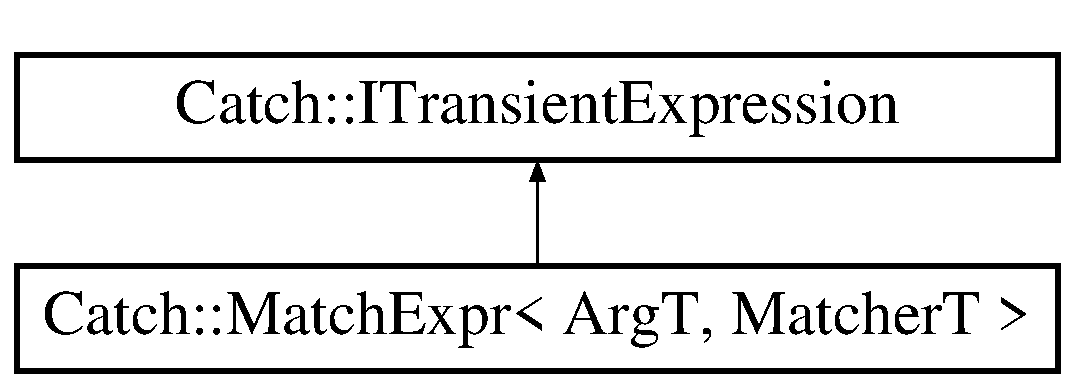
\includegraphics[height=2.000000cm]{class_catch_1_1_match_expr}
\end{center}
\end{figure}
\subsection*{Public Member Functions}
\begin{DoxyCompactItemize}
\item 
\mbox{\hyperlink{class_catch_1_1_match_expr_ae55ee9bf46c8676c65e9df291a98c345}{Match\+Expr}} (ArgT const \&arg, MatcherT const \&matcher, \mbox{\hyperlink{class_catch_1_1_string_ref}{String\+Ref}} const \&matcher\+String)
\item 
void \mbox{\hyperlink{class_catch_1_1_match_expr_ad3e41adb597750b2219bb37e51185629}{stream\+Reconstructed\+Expression}} (std\+::ostream \&os) const override
\end{DoxyCompactItemize}
\subsection*{Additional Inherited Members}


\subsection{Constructor \& Destructor Documentation}
\mbox{\Hypertarget{class_catch_1_1_match_expr_ae55ee9bf46c8676c65e9df291a98c345}\label{class_catch_1_1_match_expr_ae55ee9bf46c8676c65e9df291a98c345}} 
\index{Catch\+::\+Match\+Expr@{Catch\+::\+Match\+Expr}!Match\+Expr@{Match\+Expr}}
\index{Match\+Expr@{Match\+Expr}!Catch\+::\+Match\+Expr@{Catch\+::\+Match\+Expr}}
\subsubsection{\texorpdfstring{Match\+Expr()}{MatchExpr()}}
{\footnotesize\ttfamily template$<$typename ArgT, typename MatcherT$>$ \\
\mbox{\hyperlink{class_catch_1_1_match_expr}{Catch\+::\+Match\+Expr}}$<$ ArgT, MatcherT $>$\+::\mbox{\hyperlink{class_catch_1_1_match_expr}{Match\+Expr}} (\begin{DoxyParamCaption}\item[{ArgT const \&}]{arg,  }\item[{MatcherT const \&}]{matcher,  }\item[{\mbox{\hyperlink{class_catch_1_1_string_ref}{String\+Ref}} const \&}]{matcher\+String }\end{DoxyParamCaption})\hspace{0.3cm}{\ttfamily [inline]}}



\subsection{Member Function Documentation}
\mbox{\Hypertarget{class_catch_1_1_match_expr_ad3e41adb597750b2219bb37e51185629}\label{class_catch_1_1_match_expr_ad3e41adb597750b2219bb37e51185629}} 
\index{Catch\+::\+Match\+Expr@{Catch\+::\+Match\+Expr}!stream\+Reconstructed\+Expression@{stream\+Reconstructed\+Expression}}
\index{stream\+Reconstructed\+Expression@{stream\+Reconstructed\+Expression}!Catch\+::\+Match\+Expr@{Catch\+::\+Match\+Expr}}
\subsubsection{\texorpdfstring{stream\+Reconstructed\+Expression()}{streamReconstructedExpression()}}
{\footnotesize\ttfamily template$<$typename ArgT, typename MatcherT$>$ \\
void \mbox{\hyperlink{class_catch_1_1_match_expr}{Catch\+::\+Match\+Expr}}$<$ ArgT, MatcherT $>$\+::stream\+Reconstructed\+Expression (\begin{DoxyParamCaption}\item[{std\+::ostream \&}]{os }\end{DoxyParamCaption}) const\hspace{0.3cm}{\ttfamily [inline]}, {\ttfamily [override]}, {\ttfamily [virtual]}}



Implements \mbox{\hyperlink{struct_catch_1_1_i_transient_expression_aabe1889df9c6e639a24afb08d8a0fe9e}{Catch\+::\+I\+Transient\+Expression}}.



The documentation for this class was generated from the following file\+:\begin{DoxyCompactItemize}
\item 
D\+:/kouluhommat/\+Advanced Object-\/\+Oriented Programming/lopputyö/\+Battleship/\+Battleship/\mbox{\hyperlink{catch_8hpp}{catch.\+hpp}}\end{DoxyCompactItemize}

\hypertarget{struct_catch_1_1_matchers_1_1_impl_1_1_match_not_of}{}\section{Catch\+:\+:Matchers\+:\+:Impl\+:\+:Match\+Not\+Of$<$ ArgT $>$ Struct Template Reference}
\label{struct_catch_1_1_matchers_1_1_impl_1_1_match_not_of}\index{Catch\+::\+Matchers\+::\+Impl\+::\+Match\+Not\+Of$<$ Arg\+T $>$@{Catch\+::\+Matchers\+::\+Impl\+::\+Match\+Not\+Of$<$ Arg\+T $>$}}


{\ttfamily \#include $<$catch.\+hpp$>$}

Inheritance diagram for Catch\+:\+:Matchers\+:\+:Impl\+:\+:Match\+Not\+Of$<$ ArgT $>$\+:\begin{figure}[H]
\begin{center}
\leavevmode
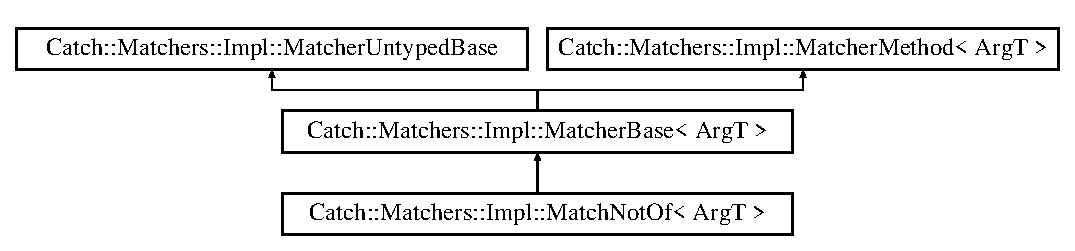
\includegraphics[height=2.926829cm]{struct_catch_1_1_matchers_1_1_impl_1_1_match_not_of}
\end{center}
\end{figure}
\subsection*{Public Member Functions}
\begin{DoxyCompactItemize}
\item 
\mbox{\hyperlink{struct_catch_1_1_matchers_1_1_impl_1_1_match_not_of_a47afdd9e4c3354cef85adc3186097ae4}{Match\+Not\+Of}} (\mbox{\hyperlink{struct_catch_1_1_matchers_1_1_impl_1_1_matcher_base}{Matcher\+Base}}$<$ ArgT $>$ const \&underlying\+Matcher)
\item 
bool \mbox{\hyperlink{struct_catch_1_1_matchers_1_1_impl_1_1_match_not_of_a181d693c0258e582d80dc6117a1f2b66}{match}} (ArgT const \&arg) const override
\item 
std\+::string \mbox{\hyperlink{struct_catch_1_1_matchers_1_1_impl_1_1_match_not_of_ac5fb4ef6a9069d23a4098c3c818f06b0}{describe}} () const override
\end{DoxyCompactItemize}
\subsection*{Public Attributes}
\begin{DoxyCompactItemize}
\item 
\mbox{\hyperlink{struct_catch_1_1_matchers_1_1_impl_1_1_matcher_base}{Matcher\+Base}}$<$ ArgT $>$ const  \& \mbox{\hyperlink{struct_catch_1_1_matchers_1_1_impl_1_1_match_not_of_af7ac67f112b0e93796b048a47329aad4}{m\+\_\+underlying\+Matcher}}
\end{DoxyCompactItemize}
\subsection*{Additional Inherited Members}


\subsection{Constructor \& Destructor Documentation}
\mbox{\Hypertarget{struct_catch_1_1_matchers_1_1_impl_1_1_match_not_of_a47afdd9e4c3354cef85adc3186097ae4}\label{struct_catch_1_1_matchers_1_1_impl_1_1_match_not_of_a47afdd9e4c3354cef85adc3186097ae4}} 
\index{Catch\+::\+Matchers\+::\+Impl\+::\+Match\+Not\+Of@{Catch\+::\+Matchers\+::\+Impl\+::\+Match\+Not\+Of}!Match\+Not\+Of@{Match\+Not\+Of}}
\index{Match\+Not\+Of@{Match\+Not\+Of}!Catch\+::\+Matchers\+::\+Impl\+::\+Match\+Not\+Of@{Catch\+::\+Matchers\+::\+Impl\+::\+Match\+Not\+Of}}
\subsubsection{\texorpdfstring{Match\+Not\+Of()}{MatchNotOf()}}
{\footnotesize\ttfamily template$<$typename ArgT$>$ \\
\mbox{\hyperlink{struct_catch_1_1_matchers_1_1_impl_1_1_match_not_of}{Catch\+::\+Matchers\+::\+Impl\+::\+Match\+Not\+Of}}$<$ ArgT $>$\+::\mbox{\hyperlink{struct_catch_1_1_matchers_1_1_impl_1_1_match_not_of}{Match\+Not\+Of}} (\begin{DoxyParamCaption}\item[{\mbox{\hyperlink{struct_catch_1_1_matchers_1_1_impl_1_1_matcher_base}{Matcher\+Base}}$<$ ArgT $>$ const \&}]{underlying\+Matcher }\end{DoxyParamCaption})\hspace{0.3cm}{\ttfamily [inline]}}



\subsection{Member Function Documentation}
\mbox{\Hypertarget{struct_catch_1_1_matchers_1_1_impl_1_1_match_not_of_ac5fb4ef6a9069d23a4098c3c818f06b0}\label{struct_catch_1_1_matchers_1_1_impl_1_1_match_not_of_ac5fb4ef6a9069d23a4098c3c818f06b0}} 
\index{Catch\+::\+Matchers\+::\+Impl\+::\+Match\+Not\+Of@{Catch\+::\+Matchers\+::\+Impl\+::\+Match\+Not\+Of}!describe@{describe}}
\index{describe@{describe}!Catch\+::\+Matchers\+::\+Impl\+::\+Match\+Not\+Of@{Catch\+::\+Matchers\+::\+Impl\+::\+Match\+Not\+Of}}
\subsubsection{\texorpdfstring{describe()}{describe()}}
{\footnotesize\ttfamily template$<$typename ArgT$>$ \\
std\+::string \mbox{\hyperlink{struct_catch_1_1_matchers_1_1_impl_1_1_match_not_of}{Catch\+::\+Matchers\+::\+Impl\+::\+Match\+Not\+Of}}$<$ ArgT $>$\+::describe (\begin{DoxyParamCaption}{ }\end{DoxyParamCaption}) const\hspace{0.3cm}{\ttfamily [inline]}, {\ttfamily [override]}, {\ttfamily [virtual]}}



Implements \mbox{\hyperlink{class_catch_1_1_matchers_1_1_impl_1_1_matcher_untyped_base_a91d3a907dbfcbb596077df24f6e11fe2}{Catch\+::\+Matchers\+::\+Impl\+::\+Matcher\+Untyped\+Base}}.

\mbox{\Hypertarget{struct_catch_1_1_matchers_1_1_impl_1_1_match_not_of_a181d693c0258e582d80dc6117a1f2b66}\label{struct_catch_1_1_matchers_1_1_impl_1_1_match_not_of_a181d693c0258e582d80dc6117a1f2b66}} 
\index{Catch\+::\+Matchers\+::\+Impl\+::\+Match\+Not\+Of@{Catch\+::\+Matchers\+::\+Impl\+::\+Match\+Not\+Of}!match@{match}}
\index{match@{match}!Catch\+::\+Matchers\+::\+Impl\+::\+Match\+Not\+Of@{Catch\+::\+Matchers\+::\+Impl\+::\+Match\+Not\+Of}}
\subsubsection{\texorpdfstring{match()}{match()}}
{\footnotesize\ttfamily template$<$typename ArgT$>$ \\
bool \mbox{\hyperlink{struct_catch_1_1_matchers_1_1_impl_1_1_match_not_of}{Catch\+::\+Matchers\+::\+Impl\+::\+Match\+Not\+Of}}$<$ ArgT $>$\+::match (\begin{DoxyParamCaption}\item[{ArgT const \&}]{arg }\end{DoxyParamCaption}) const\hspace{0.3cm}{\ttfamily [inline]}, {\ttfamily [override]}, {\ttfamily [virtual]}}



Implements \mbox{\hyperlink{struct_catch_1_1_matchers_1_1_impl_1_1_matcher_method_ae0920ff9e817acf08e1bb0cbcb044e30}{Catch\+::\+Matchers\+::\+Impl\+::\+Matcher\+Method$<$ Arg\+T $>$}}.



\subsection{Member Data Documentation}
\mbox{\Hypertarget{struct_catch_1_1_matchers_1_1_impl_1_1_match_not_of_af7ac67f112b0e93796b048a47329aad4}\label{struct_catch_1_1_matchers_1_1_impl_1_1_match_not_of_af7ac67f112b0e93796b048a47329aad4}} 
\index{Catch\+::\+Matchers\+::\+Impl\+::\+Match\+Not\+Of@{Catch\+::\+Matchers\+::\+Impl\+::\+Match\+Not\+Of}!m\+\_\+underlying\+Matcher@{m\+\_\+underlying\+Matcher}}
\index{m\+\_\+underlying\+Matcher@{m\+\_\+underlying\+Matcher}!Catch\+::\+Matchers\+::\+Impl\+::\+Match\+Not\+Of@{Catch\+::\+Matchers\+::\+Impl\+::\+Match\+Not\+Of}}
\subsubsection{\texorpdfstring{m\+\_\+underlying\+Matcher}{m\_underlyingMatcher}}
{\footnotesize\ttfamily template$<$typename ArgT$>$ \\
\mbox{\hyperlink{struct_catch_1_1_matchers_1_1_impl_1_1_matcher_base}{Matcher\+Base}}$<$ArgT$>$ const\& \mbox{\hyperlink{struct_catch_1_1_matchers_1_1_impl_1_1_match_not_of}{Catch\+::\+Matchers\+::\+Impl\+::\+Match\+Not\+Of}}$<$ ArgT $>$\+::m\+\_\+underlying\+Matcher}



The documentation for this struct was generated from the following file\+:\begin{DoxyCompactItemize}
\item 
D\+:/kouluhommat/\+Advanced Object-\/\+Oriented Programming/lopputyö/\+Battleship/\+Battleship/\mbox{\hyperlink{catch_8hpp}{catch.\+hpp}}\end{DoxyCompactItemize}

\hypertarget{class_medium_player}{}\section{Medium\+Player Class Reference}
\label{class_medium_player}\index{Medium\+Player@{Medium\+Player}}


{\ttfamily \#include $<$Player.\+h$>$}

Inheritance diagram for Medium\+Player\+:\begin{figure}[H]
\begin{center}
\leavevmode
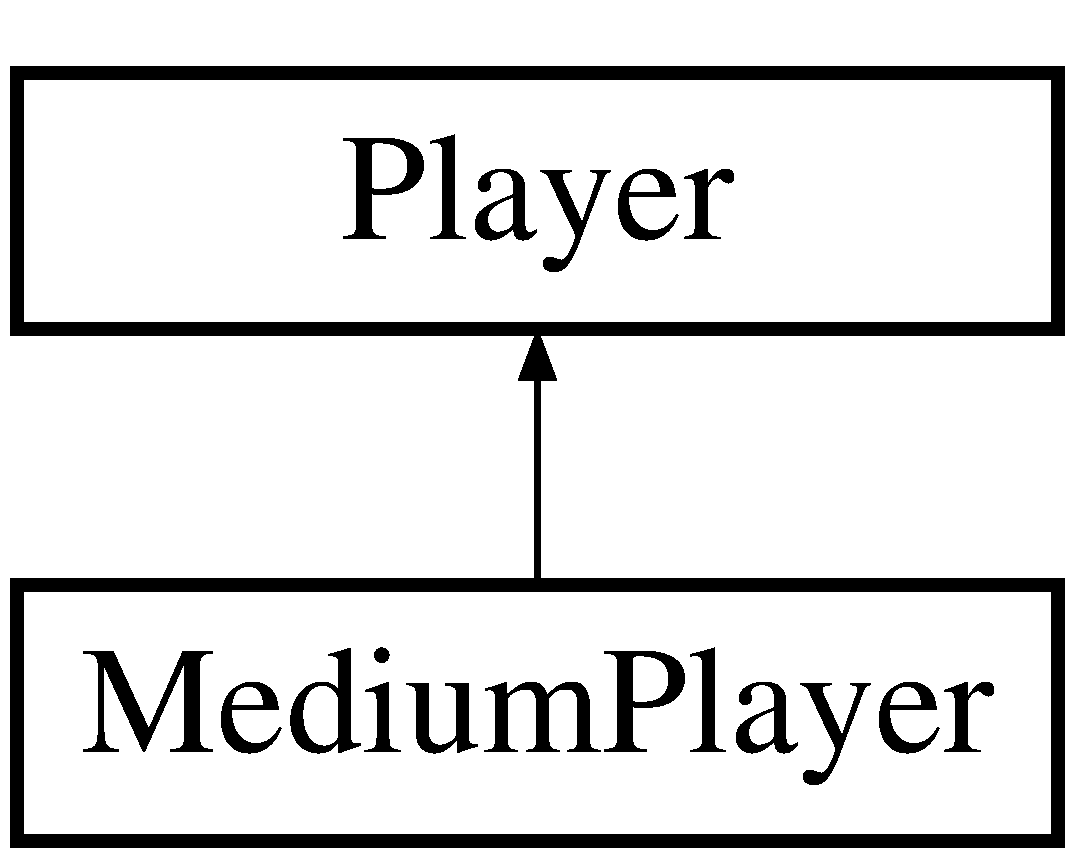
\includegraphics[height=2.000000cm]{class_medium_player}
\end{center}
\end{figure}
\subsection*{Public Member Functions}
\begin{DoxyCompactItemize}
\item 
\mbox{\hyperlink{class_player}{Player}} $\ast$ \mbox{\hyperlink{class_medium_player_a6a51f6bab42f57e8af235f2ab196d74e}{create}} (std\+::string nm, const \mbox{\hyperlink{class_game}{Game}} \&g)
\item 
\mbox{\Hypertarget{class_medium_player_a76923857c4fa54d192ed4644c72bce2d}\label{class_medium_player_a76923857c4fa54d192ed4644c72bce2d}} 
\mbox{\hyperlink{class_medium_player_a76923857c4fa54d192ed4644c72bce2d}{Medium\+Player}} (std\+::string nm, const \mbox{\hyperlink{class_game}{Game}} \&g)
\begin{DoxyCompactList}\small\item\em Constructor for medium bot. \end{DoxyCompactList}\item 
virtual bool \mbox{\hyperlink{class_medium_player_ac4d4748e2c27a2a51033bbce9f12de26}{place\+Ships}} (\mbox{\hyperlink{class_board}{Board}} \&b)
\begin{DoxyCompactList}\small\item\em Destructor for medium player. \end{DoxyCompactList}\item 
virtual \mbox{\hyperlink{class_point}{Point}} \mbox{\hyperlink{class_medium_player_a2e99d57f30f3f7f929840b8cda16527d}{recommend}} ()
\item 
virtual void \mbox{\hyperlink{class_medium_player_aeadd8498cba5c447afbb5a0eb7408285}{record\+Result}} (\mbox{\hyperlink{class_point}{Point}} p, bool valid\+Shot, bool hit, bool destroyed, int ship\+ID)
\item 
virtual void \mbox{\hyperlink{class_medium_player_a6183d4a8fe3d68419afcfa9e33cd5928}{record\+Opponent}} (\mbox{\hyperlink{class_point}{Point}} p)
\item 
bool \mbox{\hyperlink{class_medium_player_a502c34f56cfe60def6d01de7c4f300e2}{medium\+Helper}} (\mbox{\hyperlink{class_board}{Board}} \&b, int ship\+ID, int r, int c, \mbox{\hyperlink{_globals_8h_a224b9163917ac32fc95a60d8c1eec3aa}{Direction}} ld)
\begin{DoxyCompactList}\small\item\em Method for helping medium bot\textquotesingle{}s operations. \end{DoxyCompactList}\item 
\mbox{\Hypertarget{class_medium_player_a90a8cd5feeaa759043af77afe266907c}\label{class_medium_player_a90a8cd5feeaa759043af77afe266907c}} 
virtual bool {\bfseries get\+State} () const
\item 
\mbox{\Hypertarget{class_medium_player_ae0f69d678d6567e09baed0350468be61}\label{class_medium_player_ae0f69d678d6567e09baed0350468be61}} 
virtual void \mbox{\hyperlink{class_medium_player_ae0f69d678d6567e09baed0350468be61}{change\+State}} (bool state)
\begin{DoxyCompactList}\small\item\em Getter for the last state. \end{DoxyCompactList}\item 
\mbox{\Hypertarget{class_medium_player_abd585986250a5b713d6a554ea70e3ba6}\label{class_medium_player_abd585986250a5b713d6a554ea70e3ba6}} 
virtual \mbox{\hyperlink{class_point}{Point}} \mbox{\hyperlink{class_medium_player_abd585986250a5b713d6a554ea70e3ba6}{get\+LastP}} () const
\begin{DoxyCompactList}\small\item\em Method for changing state. \end{DoxyCompactList}\item 
virtual void \mbox{\hyperlink{class_medium_player_afc952f7dac91d979743154c021d8dee8}{change\+LastP}} (\mbox{\hyperlink{class_point}{Point}} p)
\begin{DoxyCompactList}\small\item\em Method for changing last point. \end{DoxyCompactList}\item 
virtual bool \mbox{\hyperlink{class_medium_player_a0c237af510ff84898759ed2e9a9271ce}{already\+Shot}} (\mbox{\hyperlink{class_point}{Point}} p)
\begin{DoxyCompactList}\small\item\em Method for checking if player has already shot. \end{DoxyCompactList}\item 
virtual void \mbox{\hyperlink{class_medium_player_a4cd5cbf0327e002112c80a52b279358f}{add\+Point}} (\mbox{\hyperlink{class_point}{Point}} p)
\begin{DoxyCompactList}\small\item\em Method for adding point into shots. \end{DoxyCompactList}\end{DoxyCompactItemize}


\subsection{Detailed Description}
\mbox{\hyperlink{class_medium_player}{Medium\+Player}}\+: class implementation for player class that\textquotesingle{}s controlled by medium bot 

\subsection{Member Function Documentation}
\mbox{\Hypertarget{class_medium_player_a4cd5cbf0327e002112c80a52b279358f}\label{class_medium_player_a4cd5cbf0327e002112c80a52b279358f}} 
\index{Medium\+Player@{Medium\+Player}!add\+Point@{add\+Point}}
\index{add\+Point@{add\+Point}!Medium\+Player@{Medium\+Player}}
\subsubsection{\texorpdfstring{add\+Point()}{addPoint()}}
{\footnotesize\ttfamily void Medium\+Player\+::add\+Point (\begin{DoxyParamCaption}\item[{\mbox{\hyperlink{class_point}{Point}}}]{p }\end{DoxyParamCaption})\hspace{0.3cm}{\ttfamily [virtual]}}



Method for adding point into shots. 

Method for adding point into shots 
\begin{DoxyParams}{Parameters}
{\em p} & \mbox{\hyperlink{class_point}{Point}} for target cell \\
\hline
\end{DoxyParams}
\mbox{\Hypertarget{class_medium_player_a0c237af510ff84898759ed2e9a9271ce}\label{class_medium_player_a0c237af510ff84898759ed2e9a9271ce}} 
\index{Medium\+Player@{Medium\+Player}!already\+Shot@{already\+Shot}}
\index{already\+Shot@{already\+Shot}!Medium\+Player@{Medium\+Player}}
\subsubsection{\texorpdfstring{already\+Shot()}{alreadyShot()}}
{\footnotesize\ttfamily bool Medium\+Player\+::already\+Shot (\begin{DoxyParamCaption}\item[{\mbox{\hyperlink{class_point}{Point}}}]{p }\end{DoxyParamCaption})\hspace{0.3cm}{\ttfamily [virtual]}}



Method for checking if player has already shot. 

Method for checking if medium bot has already shot 
\begin{DoxyParams}{Parameters}
{\em p} & \mbox{\hyperlink{class_point}{Point}} containing target cell \\
\hline
\end{DoxyParams}
Checks if given point\textquotesingle{}s rows and columns are greater than game\textquotesingle{}s or less than 0

Loops through number of shots

Checks if point\textquotesingle{}s rows and columns correspond to shot\textquotesingle{}s rows and columns \mbox{\Hypertarget{class_medium_player_afc952f7dac91d979743154c021d8dee8}\label{class_medium_player_afc952f7dac91d979743154c021d8dee8}} 
\index{Medium\+Player@{Medium\+Player}!change\+LastP@{change\+LastP}}
\index{change\+LastP@{change\+LastP}!Medium\+Player@{Medium\+Player}}
\subsubsection{\texorpdfstring{change\+Last\+P()}{changeLastP()}}
{\footnotesize\ttfamily virtual void Medium\+Player\+::change\+LastP (\begin{DoxyParamCaption}\item[{\mbox{\hyperlink{class_point}{Point}}}]{p }\end{DoxyParamCaption})\hspace{0.3cm}{\ttfamily [inline]}, {\ttfamily [virtual]}}



Method for changing last point. 

Getter for last point \mbox{\Hypertarget{class_medium_player_a6a51f6bab42f57e8af235f2ab196d74e}\label{class_medium_player_a6a51f6bab42f57e8af235f2ab196d74e}} 
\index{Medium\+Player@{Medium\+Player}!create@{create}}
\index{create@{create}!Medium\+Player@{Medium\+Player}}
\subsubsection{\texorpdfstring{create()}{create()}}
{\footnotesize\ttfamily \mbox{\hyperlink{class_player}{Player}}$\ast$ Medium\+Player\+::create (\begin{DoxyParamCaption}\item[{std\+::string}]{nm,  }\item[{const \mbox{\hyperlink{class_game}{Game}} \&}]{g }\end{DoxyParamCaption})\hspace{0.3cm}{\ttfamily [inline]}, {\ttfamily [virtual]}}

Pure virtual method for creating a player 
\begin{DoxyParams}{Parameters}
{\em nm} & string containing player\textquotesingle{}s name \\
\hline
{\em g} & reference to game object \\
\hline
\end{DoxyParams}


Implements \mbox{\hyperlink{class_player_a9b9133f3347894da1416953048cecdb2}{Player}}.

\mbox{\Hypertarget{class_medium_player_a502c34f56cfe60def6d01de7c4f300e2}\label{class_medium_player_a502c34f56cfe60def6d01de7c4f300e2}} 
\index{Medium\+Player@{Medium\+Player}!medium\+Helper@{medium\+Helper}}
\index{medium\+Helper@{medium\+Helper}!Medium\+Player@{Medium\+Player}}
\subsubsection{\texorpdfstring{medium\+Helper()}{mediumHelper()}}
{\footnotesize\ttfamily bool Medium\+Player\+::medium\+Helper (\begin{DoxyParamCaption}\item[{\mbox{\hyperlink{class_board}{Board}} \&}]{b,  }\item[{int}]{ship\+ID,  }\item[{int}]{r,  }\item[{int}]{c,  }\item[{\mbox{\hyperlink{_globals_8h_a224b9163917ac32fc95a60d8c1eec3aa}{Direction}}}]{ld }\end{DoxyParamCaption})}



Method for helping medium bot\textquotesingle{}s operations. 

Method for medium bot\textquotesingle{}s operations 
\begin{DoxyParams}{Parameters}
{\em b} & reference to game board object \\
\hline
{\em ship\+ID} & integer containing ship\textquotesingle{}s ID \\
\hline
{\em r} & integer containing row \\
\hline
{\em c} & integer containing column \\
\hline
{\em ld} & Direction object containing last direction \\
\hline
\end{DoxyParams}
Checks if we are at the last ship

Loops through point\textquotesingle{}s rows

Loops through point\textquotesingle{}s columns

Try to place ship horizontally

Try to place ship vertically

Checks if ship id is less than game\textquotesingle{}s number of ships -\/ 1

Loops through game\textquotesingle{}s rows

Loops through game\textquotesingle{}s columns

Try to place ship horizontally

Try to place ship vertically

Checks if method has been success

Checks if method has been success

$<$ Checks if method hasn\textquotesingle{}t been success and backtracks the move

$<$ Otherwise this is a first ship and we have failed \mbox{\Hypertarget{class_medium_player_ac4d4748e2c27a2a51033bbce9f12de26}\label{class_medium_player_ac4d4748e2c27a2a51033bbce9f12de26}} 
\index{Medium\+Player@{Medium\+Player}!place\+Ships@{place\+Ships}}
\index{place\+Ships@{place\+Ships}!Medium\+Player@{Medium\+Player}}
\subsubsection{\texorpdfstring{place\+Ships()}{placeShips()}}
{\footnotesize\ttfamily bool Medium\+Player\+::place\+Ships (\begin{DoxyParamCaption}\item[{\mbox{\hyperlink{class_board}{Board}} \&}]{b }\end{DoxyParamCaption})\hspace{0.3cm}{\ttfamily [virtual]}}



Destructor for medium player. 

Method for placing ships 
\begin{DoxyParams}{Parameters}
{\em b} & reference to game board object \\
\hline
\end{DoxyParams}
$<$ Integer for count ~\newline
~\newline
~\newline
~\newline
~\newline
~\newline
~\newline
 Loops while count is less than 50

$<$ Blocks the game board ~\newline
~\newline
~\newline
~\newline
~\newline
 Checks if medium helper is success with 0 values

$<$ Unblocks the game board

$<$ Increases count

$<$ Unblocks the game board

$<$ Unblocks the game board 

Implements \mbox{\hyperlink{class_player_ab89c1180c7314d3e19bcf4b2bed2e02a}{Player}}.

\mbox{\Hypertarget{class_medium_player_a2e99d57f30f3f7f929840b8cda16527d}\label{class_medium_player_a2e99d57f30f3f7f929840b8cda16527d}} 
\index{Medium\+Player@{Medium\+Player}!recommend@{recommend}}
\index{recommend@{recommend}!Medium\+Player@{Medium\+Player}}
\subsubsection{\texorpdfstring{recommend()}{recommend()}}
{\footnotesize\ttfamily \mbox{\hyperlink{class_point}{Point}} Medium\+Player\+::recommend (\begin{DoxyParamCaption}{ }\end{DoxyParamCaption})\hspace{0.3cm}{\ttfamily [virtual]}}

Method for recommending attack for medium bot $<$ Random integer with limit 4 + 1

$<$ \mbox{\hyperlink{class_point}{Point}} for answer cell

$<$ Random integer with limit 2

$<$ Random integer with limit 2

$<$ integer for count

Checks if state isn\textquotesingle{}t 1

Loops from 1 to 5

Checks if cells around the last point haven\textquotesingle{}t been shot

Checks if while loop finished

Checks if state is 1

Get random point

Checks if random point has already been shot

$<$ Recommends attack

$<$ Returns random point

Checks if first random integer is 0

Checks if second random integer is 1

$<$ Second random integer is 0

$<$ First random integer is 1 ~\newline
~\newline
~\newline
 Checks if second random integer is 0

$<$ First random integer is 1

Checks if answer cell has already been shot or target is OoB 

Implements \mbox{\hyperlink{class_player_a2cc7a83d11158eafd8d49d4b9f23ce56}{Player}}.

\mbox{\Hypertarget{class_medium_player_a6183d4a8fe3d68419afcfa9e33cd5928}\label{class_medium_player_a6183d4a8fe3d68419afcfa9e33cd5928}} 
\index{Medium\+Player@{Medium\+Player}!record\+Opponent@{record\+Opponent}}
\index{record\+Opponent@{record\+Opponent}!Medium\+Player@{Medium\+Player}}
\subsubsection{\texorpdfstring{record\+Opponent()}{recordOpponent()}}
{\footnotesize\ttfamily void Medium\+Player\+::record\+Opponent (\begin{DoxyParamCaption}\item[{\mbox{\hyperlink{class_point}{Point}}}]{p }\end{DoxyParamCaption})\hspace{0.3cm}{\ttfamily [virtual]}}

Method for recording opponent\textquotesingle{}s attacks 
\begin{DoxyParams}{Parameters}
{\em p} & \mbox{\hyperlink{class_point}{Point}} containing target cell \\
\hline
\end{DoxyParams}


Implements \mbox{\hyperlink{class_player_a768e14edee61e208e6fd295cdd72a49c}{Player}}.

\mbox{\Hypertarget{class_medium_player_aeadd8498cba5c447afbb5a0eb7408285}\label{class_medium_player_aeadd8498cba5c447afbb5a0eb7408285}} 
\index{Medium\+Player@{Medium\+Player}!record\+Result@{record\+Result}}
\index{record\+Result@{record\+Result}!Medium\+Player@{Medium\+Player}}
\subsubsection{\texorpdfstring{record\+Result()}{recordResult()}}
{\footnotesize\ttfamily void Medium\+Player\+::record\+Result (\begin{DoxyParamCaption}\item[{\mbox{\hyperlink{class_point}{Point}}}]{p,  }\item[{bool}]{valid\+Shot,  }\item[{bool}]{hit,  }\item[{bool}]{destroyed,  }\item[{int}]{ship\+ID }\end{DoxyParamCaption})\hspace{0.3cm}{\ttfamily [virtual]}}

Method for recording attack result 
\begin{DoxyParams}{Parameters}
{\em p} & \mbox{\hyperlink{class_point}{Point}} object of cell \\
\hline
{\em valid\+Shot} & boolean for checking if shot was valid \\
\hline
{\em hit} & boolean for checking if ship was hit \\
\hline
{\em destroyed} & boolean for checking if ship was destroyed \\
\hline
{\em ship\+ID} & integer containing ship id \\
\hline
\end{DoxyParams}
Checks if shot wasn\textquotesingle{}t valid

Checks if target cell hasn\textquotesingle{}t already been shot

$<$ Adds point into shots

$<$ Increases number of shots

Checks if ship was hit and state is 1

$<$ Last point updated

$<$ Shot hit so turn to state 2

Checks if ship was destroyed

$<$ \mbox{\hyperlink{class_ship}{Ship}} was destroyed so turn to state 1 

Implements \mbox{\hyperlink{class_player_a368527cfefaac58dc942b32658f977ed}{Player}}.



The documentation for this class was generated from the following files\+:\begin{DoxyCompactItemize}
\item 
D\+:/kouluhommat/\+Advanced Object-\/\+Oriented Programming/lopputyö/\+Battleship/\+Battleship/\mbox{\hyperlink{_player_8h}{Player.\+h}}\item 
D\+:/kouluhommat/\+Advanced Object-\/\+Oriented Programming/lopputyö/\+Battleship/\+Battleship/\mbox{\hyperlink{_player_8cpp}{Player.\+cpp}}\end{DoxyCompactItemize}

\hypertarget{struct_catch_1_1_message_builder}{}\section{Catch\+:\+:Message\+Builder Struct Reference}
\label{struct_catch_1_1_message_builder}\index{Catch\+::\+Message\+Builder@{Catch\+::\+Message\+Builder}}


{\ttfamily \#include $<$catch.\+hpp$>$}

Inheritance diagram for Catch\+:\+:Message\+Builder\+:\begin{figure}[H]
\begin{center}
\leavevmode
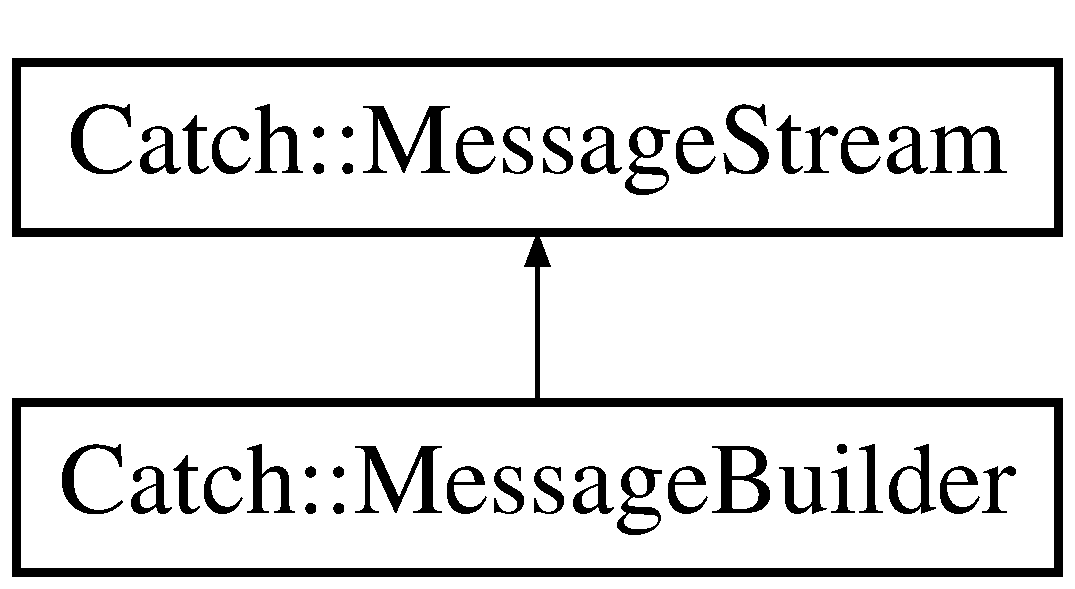
\includegraphics[height=2.000000cm]{struct_catch_1_1_message_builder}
\end{center}
\end{figure}
\subsection*{Public Member Functions}
\begin{DoxyCompactItemize}
\item 
\mbox{\hyperlink{struct_catch_1_1_message_builder_ac34832ca527a758f000ac233d32dd068}{Message\+Builder}} (\mbox{\hyperlink{class_catch_1_1_string_ref}{String\+Ref}} const \&macro\+Name, \mbox{\hyperlink{struct_catch_1_1_source_line_info}{Source\+Line\+Info}} const \&line\+Info, \mbox{\hyperlink{struct_catch_1_1_result_was_a624e1ee3661fcf6094ceef1f654601ef}{Result\+Was\+::\+Of\+Type}} type)
\item 
{\footnotesize template$<$typename T $>$ }\\\mbox{\hyperlink{struct_catch_1_1_message_builder}{Message\+Builder}} \& \mbox{\hyperlink{struct_catch_1_1_message_builder_a20fa48d069b20dddcc2d3df8abb123c1}{operator$<$$<$}} (T const \&value)
\end{DoxyCompactItemize}
\subsection*{Public Attributes}
\begin{DoxyCompactItemize}
\item 
\mbox{\hyperlink{struct_catch_1_1_message_info}{Message\+Info}} \mbox{\hyperlink{struct_catch_1_1_message_builder_a979f1c2b36d78f80ee275bfa5ba0209f}{m\+\_\+info}}
\end{DoxyCompactItemize}


\subsection{Constructor \& Destructor Documentation}
\mbox{\Hypertarget{struct_catch_1_1_message_builder_ac34832ca527a758f000ac233d32dd068}\label{struct_catch_1_1_message_builder_ac34832ca527a758f000ac233d32dd068}} 
\index{Catch\+::\+Message\+Builder@{Catch\+::\+Message\+Builder}!Message\+Builder@{Message\+Builder}}
\index{Message\+Builder@{Message\+Builder}!Catch\+::\+Message\+Builder@{Catch\+::\+Message\+Builder}}
\subsubsection{\texorpdfstring{Message\+Builder()}{MessageBuilder()}}
{\footnotesize\ttfamily Catch\+::\+Message\+Builder\+::\+Message\+Builder (\begin{DoxyParamCaption}\item[{\mbox{\hyperlink{class_catch_1_1_string_ref}{String\+Ref}} const \&}]{macro\+Name,  }\item[{\mbox{\hyperlink{struct_catch_1_1_source_line_info}{Source\+Line\+Info}} const \&}]{line\+Info,  }\item[{\mbox{\hyperlink{struct_catch_1_1_result_was_a624e1ee3661fcf6094ceef1f654601ef}{Result\+Was\+::\+Of\+Type}}}]{type }\end{DoxyParamCaption})}



\subsection{Member Function Documentation}
\mbox{\Hypertarget{struct_catch_1_1_message_builder_a20fa48d069b20dddcc2d3df8abb123c1}\label{struct_catch_1_1_message_builder_a20fa48d069b20dddcc2d3df8abb123c1}} 
\index{Catch\+::\+Message\+Builder@{Catch\+::\+Message\+Builder}!operator$<$$<$@{operator$<$$<$}}
\index{operator$<$$<$@{operator$<$$<$}!Catch\+::\+Message\+Builder@{Catch\+::\+Message\+Builder}}
\subsubsection{\texorpdfstring{operator$<$$<$()}{operator<<()}}
{\footnotesize\ttfamily template$<$typename T $>$ \\
\mbox{\hyperlink{struct_catch_1_1_message_builder}{Message\+Builder}}\& Catch\+::\+Message\+Builder\+::operator$<$$<$ (\begin{DoxyParamCaption}\item[{T const \&}]{value }\end{DoxyParamCaption})\hspace{0.3cm}{\ttfamily [inline]}}



\subsection{Member Data Documentation}
\mbox{\Hypertarget{struct_catch_1_1_message_builder_a979f1c2b36d78f80ee275bfa5ba0209f}\label{struct_catch_1_1_message_builder_a979f1c2b36d78f80ee275bfa5ba0209f}} 
\index{Catch\+::\+Message\+Builder@{Catch\+::\+Message\+Builder}!m\+\_\+info@{m\+\_\+info}}
\index{m\+\_\+info@{m\+\_\+info}!Catch\+::\+Message\+Builder@{Catch\+::\+Message\+Builder}}
\subsubsection{\texorpdfstring{m\+\_\+info}{m\_info}}
{\footnotesize\ttfamily \mbox{\hyperlink{struct_catch_1_1_message_info}{Message\+Info}} Catch\+::\+Message\+Builder\+::m\+\_\+info}



The documentation for this struct was generated from the following file\+:\begin{DoxyCompactItemize}
\item 
D\+:/kouluhommat/\+Advanced Object-\/\+Oriented Programming/lopputyö/\+Battleship/\+Battleship/\mbox{\hyperlink{catch_8hpp}{catch.\+hpp}}\end{DoxyCompactItemize}

\hypertarget{struct_catch_1_1_message_info}{}\section{Catch\+:\+:Message\+Info Struct Reference}
\label{struct_catch_1_1_message_info}\index{Catch\+::\+Message\+Info@{Catch\+::\+Message\+Info}}
\subsection*{Public Member Functions}
\begin{DoxyCompactItemize}
\item 
\mbox{\Hypertarget{struct_catch_1_1_message_info_afac7a84a9e8655428035a3c5418044f0}\label{struct_catch_1_1_message_info_afac7a84a9e8655428035a3c5418044f0}} 
{\bfseries Message\+Info} (\mbox{\hyperlink{class_catch_1_1_string_ref}{String\+Ref}} const \&\+\_\+macro\+Name, \mbox{\hyperlink{struct_catch_1_1_source_line_info}{Source\+Line\+Info}} const \&\+\_\+line\+Info, Result\+Was\+::\+Of\+Type \+\_\+type)
\item 
\mbox{\Hypertarget{struct_catch_1_1_message_info_af4b37f2172ba55395813b4bb6bbbde1a}\label{struct_catch_1_1_message_info_af4b37f2172ba55395813b4bb6bbbde1a}} 
bool {\bfseries operator==} (\mbox{\hyperlink{struct_catch_1_1_message_info}{Message\+Info}} const \&other) const
\item 
\mbox{\Hypertarget{struct_catch_1_1_message_info_a8254cb8fca2da02a29a9843cdcb79df1}\label{struct_catch_1_1_message_info_a8254cb8fca2da02a29a9843cdcb79df1}} 
bool {\bfseries operator$<$} (\mbox{\hyperlink{struct_catch_1_1_message_info}{Message\+Info}} const \&other) const
\end{DoxyCompactItemize}
\subsection*{Public Attributes}
\begin{DoxyCompactItemize}
\item 
\mbox{\Hypertarget{struct_catch_1_1_message_info_a3ee7cd41def0989d2193bad7101436a0}\label{struct_catch_1_1_message_info_a3ee7cd41def0989d2193bad7101436a0}} 
\mbox{\hyperlink{class_catch_1_1_string_ref}{String\+Ref}} {\bfseries macro\+Name}
\item 
\mbox{\Hypertarget{struct_catch_1_1_message_info_ab6cd06e050bf426c6577502a5c50e256}\label{struct_catch_1_1_message_info_ab6cd06e050bf426c6577502a5c50e256}} 
std\+::string {\bfseries message}
\item 
\mbox{\Hypertarget{struct_catch_1_1_message_info_a985165328723e599696ebd8e43195cc5}\label{struct_catch_1_1_message_info_a985165328723e599696ebd8e43195cc5}} 
\mbox{\hyperlink{struct_catch_1_1_source_line_info}{Source\+Line\+Info}} {\bfseries line\+Info}
\item 
\mbox{\Hypertarget{struct_catch_1_1_message_info_ae928b9117465c696e45951d9d0284e78}\label{struct_catch_1_1_message_info_ae928b9117465c696e45951d9d0284e78}} 
Result\+Was\+::\+Of\+Type {\bfseries type}
\item 
\mbox{\Hypertarget{struct_catch_1_1_message_info_a7f4f57ea21e50160adefce7b68a781d6}\label{struct_catch_1_1_message_info_a7f4f57ea21e50160adefce7b68a781d6}} 
unsigned int {\bfseries sequence}
\end{DoxyCompactItemize}


The documentation for this struct was generated from the following file\+:\begin{DoxyCompactItemize}
\item 
D\+:/kouluhommat/\+Advanced Object-\/\+Oriented Programming/lopputyö/\+Battleship/\+Battleship/catch.\+hpp\end{DoxyCompactItemize}

\hypertarget{struct_catch_1_1_message_stream}{}\section{Catch\+:\+:Message\+Stream Struct Reference}
\label{struct_catch_1_1_message_stream}\index{Catch\+::\+Message\+Stream@{Catch\+::\+Message\+Stream}}
Inheritance diagram for Catch\+:\+:Message\+Stream\+:\begin{figure}[H]
\begin{center}
\leavevmode
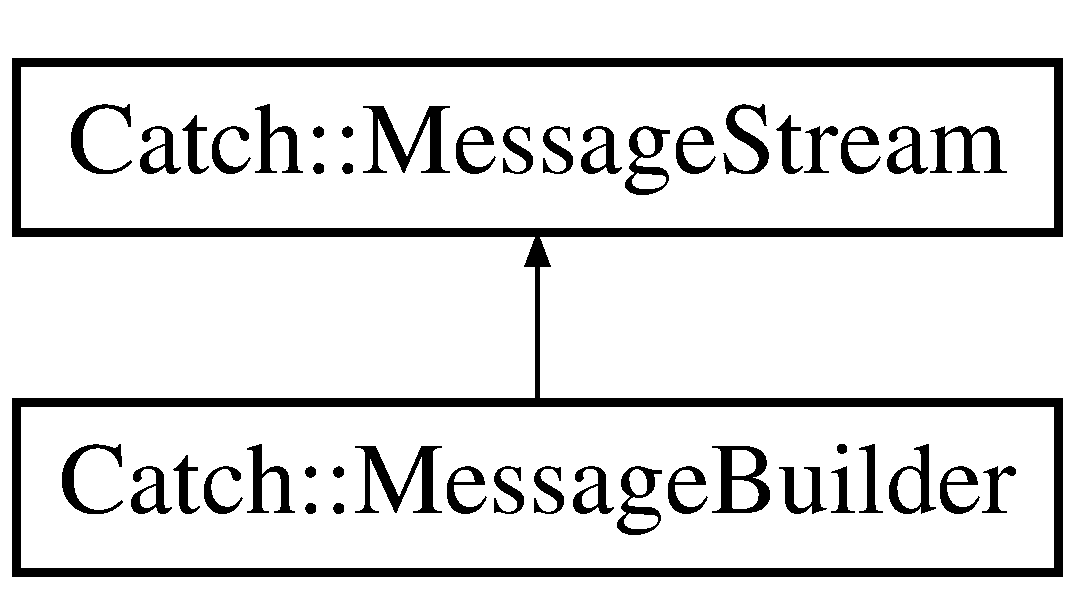
\includegraphics[height=2.000000cm]{struct_catch_1_1_message_stream}
\end{center}
\end{figure}
\subsection*{Public Member Functions}
\begin{DoxyCompactItemize}
\item 
\mbox{\Hypertarget{struct_catch_1_1_message_stream_a554c4aff5925a077e9fe9d858217428d}\label{struct_catch_1_1_message_stream_a554c4aff5925a077e9fe9d858217428d}} 
{\footnotesize template$<$typename T $>$ }\\\mbox{\hyperlink{struct_catch_1_1_message_stream}{Message\+Stream}} \& {\bfseries operator$<$$<$} (T const \&value)
\end{DoxyCompactItemize}
\subsection*{Public Attributes}
\begin{DoxyCompactItemize}
\item 
\mbox{\Hypertarget{struct_catch_1_1_message_stream_a9202520faed8882ef469db9f353ec578}\label{struct_catch_1_1_message_stream_a9202520faed8882ef469db9f353ec578}} 
\mbox{\hyperlink{class_catch_1_1_reusable_string_stream}{Reusable\+String\+Stream}} {\bfseries m\+\_\+stream}
\end{DoxyCompactItemize}


The documentation for this struct was generated from the following file\+:\begin{DoxyCompactItemize}
\item 
D\+:/kouluhommat/\+Advanced Object-\/\+Oriented Programming/lopputyö/\+Battleship/\+Battleship/catch.\+hpp\end{DoxyCompactItemize}

\hypertarget{struct_catch_1_1_name_and_tags}{}\section{Catch\+:\+:Name\+And\+Tags Struct Reference}
\label{struct_catch_1_1_name_and_tags}\index{Catch\+::\+Name\+And\+Tags@{Catch\+::\+Name\+And\+Tags}}
\subsection*{Public Member Functions}
\begin{DoxyCompactItemize}
\item 
\mbox{\Hypertarget{struct_catch_1_1_name_and_tags_ab585111e615ce8c504a2b9630de8ee94}\label{struct_catch_1_1_name_and_tags_ab585111e615ce8c504a2b9630de8ee94}} 
{\bfseries Name\+And\+Tags} (\mbox{\hyperlink{class_catch_1_1_string_ref}{String\+Ref}} const \&name\+\_\+=\mbox{\hyperlink{class_catch_1_1_string_ref}{String\+Ref}}(), \mbox{\hyperlink{class_catch_1_1_string_ref}{String\+Ref}} const \&tags\+\_\+=\mbox{\hyperlink{class_catch_1_1_string_ref}{String\+Ref}}()) noexcept
\end{DoxyCompactItemize}
\subsection*{Public Attributes}
\begin{DoxyCompactItemize}
\item 
\mbox{\Hypertarget{struct_catch_1_1_name_and_tags_a7cbea60e0cebfa622c667008eb011420}\label{struct_catch_1_1_name_and_tags_a7cbea60e0cebfa622c667008eb011420}} 
\mbox{\hyperlink{class_catch_1_1_string_ref}{String\+Ref}} {\bfseries name}
\item 
\mbox{\Hypertarget{struct_catch_1_1_name_and_tags_a74062ed1138834a348424eb7ed900c57}\label{struct_catch_1_1_name_and_tags_a74062ed1138834a348424eb7ed900c57}} 
\mbox{\hyperlink{class_catch_1_1_string_ref}{String\+Ref}} {\bfseries tags}
\end{DoxyCompactItemize}


The documentation for this struct was generated from the following file\+:\begin{DoxyCompactItemize}
\item 
D\+:/kouluhommat/\+Advanced Object-\/\+Oriented Programming/lopputyö/\+Battleship/\+Battleship/catch.\+hpp\end{DoxyCompactItemize}

\hypertarget{class_catch_1_1_non_copyable}{}\section{Catch\+:\+:Non\+Copyable Class Reference}
\label{class_catch_1_1_non_copyable}\index{Catch\+::\+Non\+Copyable@{Catch\+::\+Non\+Copyable}}


{\ttfamily \#include $<$catch.\+hpp$>$}

Inheritance diagram for Catch\+:\+:Non\+Copyable\+:\begin{figure}[H]
\begin{center}
\leavevmode
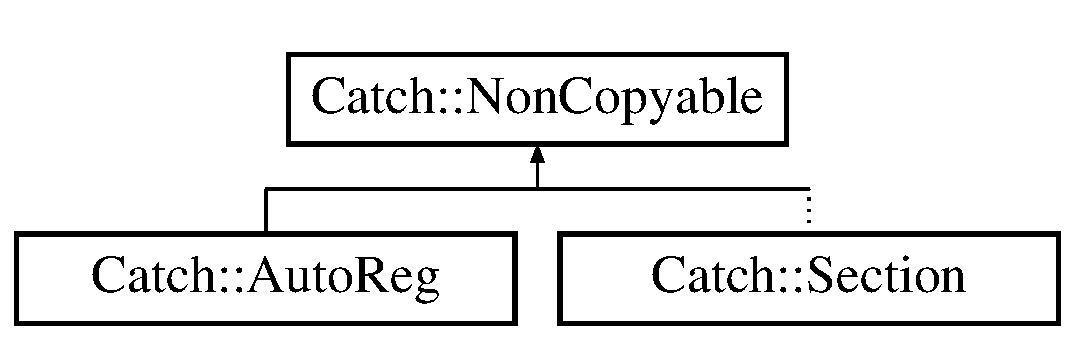
\includegraphics[height=2.000000cm]{class_catch_1_1_non_copyable}
\end{center}
\end{figure}
\subsection*{Protected Member Functions}
\begin{DoxyCompactItemize}
\item 
\mbox{\hyperlink{class_catch_1_1_non_copyable_a4b492dd5753f9952350fb64dc6cb9fe2}{Non\+Copyable}} ()
\item 
virtual \mbox{\hyperlink{class_catch_1_1_non_copyable_a81254677280fef337eb4a676e91e3293}{$\sim$\+Non\+Copyable}} ()
\end{DoxyCompactItemize}


\subsection{Constructor \& Destructor Documentation}
\mbox{\Hypertarget{class_catch_1_1_non_copyable_a4b492dd5753f9952350fb64dc6cb9fe2}\label{class_catch_1_1_non_copyable_a4b492dd5753f9952350fb64dc6cb9fe2}} 
\index{Catch\+::\+Non\+Copyable@{Catch\+::\+Non\+Copyable}!Non\+Copyable@{Non\+Copyable}}
\index{Non\+Copyable@{Non\+Copyable}!Catch\+::\+Non\+Copyable@{Catch\+::\+Non\+Copyable}}
\subsubsection{\texorpdfstring{Non\+Copyable()}{NonCopyable()}}
{\footnotesize\ttfamily Catch\+::\+Non\+Copyable\+::\+Non\+Copyable (\begin{DoxyParamCaption}{ }\end{DoxyParamCaption})\hspace{0.3cm}{\ttfamily [protected]}}

\mbox{\Hypertarget{class_catch_1_1_non_copyable_a81254677280fef337eb4a676e91e3293}\label{class_catch_1_1_non_copyable_a81254677280fef337eb4a676e91e3293}} 
\index{Catch\+::\+Non\+Copyable@{Catch\+::\+Non\+Copyable}!````~Non\+Copyable@{$\sim$\+Non\+Copyable}}
\index{````~Non\+Copyable@{$\sim$\+Non\+Copyable}!Catch\+::\+Non\+Copyable@{Catch\+::\+Non\+Copyable}}
\subsubsection{\texorpdfstring{$\sim$\+Non\+Copyable()}{~NonCopyable()}}
{\footnotesize\ttfamily virtual Catch\+::\+Non\+Copyable\+::$\sim$\+Non\+Copyable (\begin{DoxyParamCaption}{ }\end{DoxyParamCaption})\hspace{0.3cm}{\ttfamily [protected]}, {\ttfamily [virtual]}}



The documentation for this class was generated from the following file\+:\begin{DoxyCompactItemize}
\item 
D\+:/kouluhommat/\+Advanced Object-\/\+Oriented Programming/lopputyö/\+Battleship/\+Battleship/\mbox{\hyperlink{catch_8hpp}{catch.\+hpp}}\end{DoxyCompactItemize}

\hypertarget{struct_catch_1_1not__this__one}{}\section{Catch\+:\+:not\+\_\+this\+\_\+one Struct Reference}
\label{struct_catch_1_1not__this__one}\index{Catch\+::not\+\_\+this\+\_\+one@{Catch\+::not\+\_\+this\+\_\+one}}


The documentation for this struct was generated from the following file\+:\begin{DoxyCompactItemize}
\item 
D\+:/kouluhommat/\+Advanced Object-\/\+Oriented Programming/lopputyö/\+Battleship/\+Battleship/catch.\+hpp\end{DoxyCompactItemize}

\hypertarget{struct_catch_1_1_generators_1_1_null_generator}{}\section{Catch\+:\+:Generators\+:\+:Null\+Generator$<$ T $>$ Struct Template Reference}
\label{struct_catch_1_1_generators_1_1_null_generator}\index{Catch\+::\+Generators\+::\+Null\+Generator$<$ T $>$@{Catch\+::\+Generators\+::\+Null\+Generator$<$ T $>$}}
Inheritance diagram for Catch\+:\+:Generators\+:\+:Null\+Generator$<$ T $>$\+:\begin{figure}[H]
\begin{center}
\leavevmode
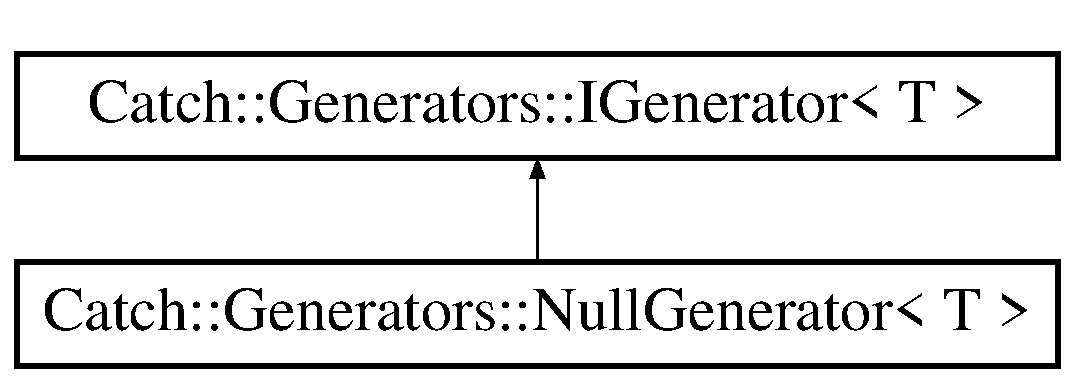
\includegraphics[height=2.000000cm]{struct_catch_1_1_generators_1_1_null_generator}
\end{center}
\end{figure}
\subsection*{Public Member Functions}
\begin{DoxyCompactItemize}
\item 
\mbox{\Hypertarget{struct_catch_1_1_generators_1_1_null_generator_a17a2cc82d644e97afded4017c7a062ef}\label{struct_catch_1_1_generators_1_1_null_generator_a17a2cc82d644e97afded4017c7a062ef}} 
auto {\bfseries get} (size\+\_\+t) const -\/$>$ T override
\end{DoxyCompactItemize}


The documentation for this struct was generated from the following file\+:\begin{DoxyCompactItemize}
\item 
D\+:/kouluhommat/\+Advanced Object-\/\+Oriented Programming/lopputyö/\+Battleship/\+Battleship/catch.\+hpp\end{DoxyCompactItemize}

\hypertarget{class_player}{}\section{Player Class Reference}
\label{class_player}\index{Player@{Player}}


Declaration for \mbox{\hyperlink{class_game}{Game}} class.  




{\ttfamily \#include $<$Player.\+h$>$}

Inheritance diagram for Player\+:\begin{figure}[H]
\begin{center}
\leavevmode
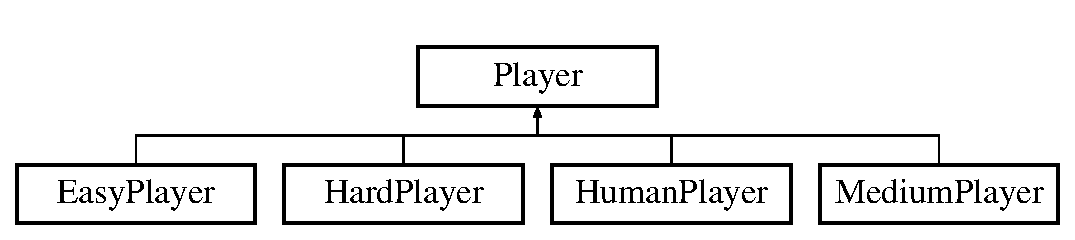
\includegraphics[height=2.000000cm]{class_player}
\end{center}
\end{figure}
\subsection*{Public Member Functions}
\begin{DoxyCompactItemize}
\item 
virtual \mbox{\hyperlink{class_player}{Player}} $\ast$ \mbox{\hyperlink{class_player_a9b9133f3347894da1416953048cecdb2}{create}} (std\+::string nm, const \mbox{\hyperlink{class_game}{Game}} \&g)=0
\item 
\mbox{\Hypertarget{class_player_adebc0e1afa34a20c0be570f8e9e3a9bf}\label{class_player_adebc0e1afa34a20c0be570f8e9e3a9bf}} 
\mbox{\hyperlink{class_player_adebc0e1afa34a20c0be570f8e9e3a9bf}{Player}} (std\+::string nm, const \mbox{\hyperlink{class_game}{Game}} \&g)
\begin{DoxyCompactList}\small\item\em Constructor for player. \end{DoxyCompactList}\item 
\mbox{\Hypertarget{class_player_a8981c201ffb2270c0b6dbd467b627376}\label{class_player_a8981c201ffb2270c0b6dbd467b627376}} 
virtual \mbox{\hyperlink{class_player_a8981c201ffb2270c0b6dbd467b627376}{$\sim$\+Player}} ()
\begin{DoxyCompactList}\small\item\em Destructor for player. \end{DoxyCompactList}\item 
\mbox{\Hypertarget{class_player_a422139ad63182cfc9f82305b87a3f9a5}\label{class_player_a422139ad63182cfc9f82305b87a3f9a5}} 
std\+::string \mbox{\hyperlink{class_player_a422139ad63182cfc9f82305b87a3f9a5}{name}} () const
\begin{DoxyCompactList}\small\item\em Getter for name. \end{DoxyCompactList}\item 
\mbox{\Hypertarget{class_player_ab4ef841709083fe60f6647ce0a7ca816}\label{class_player_ab4ef841709083fe60f6647ce0a7ca816}} 
const \mbox{\hyperlink{class_game}{Game}} \& \mbox{\hyperlink{class_player_ab4ef841709083fe60f6647ce0a7ca816}{game}} () const
\begin{DoxyCompactList}\small\item\em Getter for reference of game. \end{DoxyCompactList}\item 
\mbox{\Hypertarget{class_player_a47c5497b2d8bf5d745e85952d0bf097f}\label{class_player_a47c5497b2d8bf5d745e85952d0bf097f}} 
virtual bool \mbox{\hyperlink{class_player_a47c5497b2d8bf5d745e85952d0bf097f}{human}} () const
\begin{DoxyCompactList}\small\item\em Checks if player is human. \end{DoxyCompactList}\item 
\mbox{\Hypertarget{class_player_ab89c1180c7314d3e19bcf4b2bed2e02a}\label{class_player_ab89c1180c7314d3e19bcf4b2bed2e02a}} 
virtual bool \mbox{\hyperlink{class_player_ab89c1180c7314d3e19bcf4b2bed2e02a}{place\+Ships}} (\mbox{\hyperlink{class_board}{Board}} \&b)=0
\begin{DoxyCompactList}\small\item\em Places ships on game board. \end{DoxyCompactList}\item 
virtual \mbox{\hyperlink{class_point}{Point}} \mbox{\hyperlink{class_player_a2cc7a83d11158eafd8d49d4b9f23ce56}{recommend}} ()=0
\item 
\mbox{\Hypertarget{class_player_a368527cfefaac58dc942b32658f977ed}\label{class_player_a368527cfefaac58dc942b32658f977ed}} 
virtual void \mbox{\hyperlink{class_player_a368527cfefaac58dc942b32658f977ed}{record\+Result}} (\mbox{\hyperlink{class_point}{Point}} p, bool valid\+Shot, bool hit, bool destroyed, int ship\+ID)=0
\begin{DoxyCompactList}\small\item\em Records attack result. \end{DoxyCompactList}\item 
virtual void \mbox{\hyperlink{class_player_a768e14edee61e208e6fd295cdd72a49c}{record\+Opponent}} (\mbox{\hyperlink{class_point}{Point}} p)=0
\item 
\mbox{\Hypertarget{class_player_ae8015d1f08ba69d663cfdaea1a64d1a4}\label{class_player_ae8015d1f08ba69d663cfdaea1a64d1a4}} 
\mbox{\hyperlink{class_player_ae8015d1f08ba69d663cfdaea1a64d1a4}{Player}} (const \mbox{\hyperlink{class_player}{Player}} \&)=delete
\begin{DoxyCompactList}\small\item\em Prevents player object from being copied/assigned. \end{DoxyCompactList}\item 
\mbox{\Hypertarget{class_player_ab81d34e4adb4e329d26b1635d866462d}\label{class_player_ab81d34e4adb4e329d26b1635d866462d}} 
\mbox{\hyperlink{class_player}{Player}} \& {\bfseries operator=} (const \mbox{\hyperlink{class_player}{Player}} \&)=delete
\end{DoxyCompactItemize}


\subsection{Detailed Description}
Declaration for \mbox{\hyperlink{class_game}{Game}} class. 

\subsection{Member Function Documentation}
\mbox{\Hypertarget{class_player_a9b9133f3347894da1416953048cecdb2}\label{class_player_a9b9133f3347894da1416953048cecdb2}} 
\index{Player@{Player}!create@{create}}
\index{create@{create}!Player@{Player}}
\subsubsection{\texorpdfstring{create()}{create()}}
{\footnotesize\ttfamily virtual \mbox{\hyperlink{class_player}{Player}}$\ast$ Player\+::create (\begin{DoxyParamCaption}\item[{std\+::string}]{nm,  }\item[{const \mbox{\hyperlink{class_game}{Game}} \&}]{g }\end{DoxyParamCaption})\hspace{0.3cm}{\ttfamily [pure virtual]}}

Pure virtual method for creating a player 
\begin{DoxyParams}{Parameters}
{\em nm} & string containing player\textquotesingle{}s name \\
\hline
{\em g} & reference to game object \\
\hline
\end{DoxyParams}


Implemented in \mbox{\hyperlink{class_hard_player_ab3e76893b9c5163a33ea91b201715a98}{Hard\+Player}}, \mbox{\hyperlink{class_medium_player_a6a51f6bab42f57e8af235f2ab196d74e}{Medium\+Player}}, \mbox{\hyperlink{class_easy_player_ae927ab9f7f4d152fd457e037ad7828a5}{Easy\+Player}}, and \mbox{\hyperlink{class_human_player_ac369ccb03a62b40dcf3dc157841a965e}{Human\+Player}}.

\mbox{\Hypertarget{class_player_a2cc7a83d11158eafd8d49d4b9f23ce56}\label{class_player_a2cc7a83d11158eafd8d49d4b9f23ce56}} 
\index{Player@{Player}!recommend@{recommend}}
\index{recommend@{recommend}!Player@{Player}}
\subsubsection{\texorpdfstring{recommend()}{recommend()}}
{\footnotesize\ttfamily virtual \mbox{\hyperlink{class_point}{Point}} Player\+::recommend (\begin{DoxyParamCaption}{ }\end{DoxyParamCaption})\hspace{0.3cm}{\ttfamily [pure virtual]}}

Recommends attack 

Implemented in \mbox{\hyperlink{class_hard_player_ae1d21325a648a88f1bf51f2b0b286190}{Hard\+Player}}, \mbox{\hyperlink{class_medium_player_a2e99d57f30f3f7f929840b8cda16527d}{Medium\+Player}}, \mbox{\hyperlink{class_easy_player_a9b00f4a9acc74ff688c609bc15bdbb4d}{Easy\+Player}}, and \mbox{\hyperlink{class_human_player_a718f16f3ddeeb34c9f2e93cf1d805b46}{Human\+Player}}.

\mbox{\Hypertarget{class_player_a768e14edee61e208e6fd295cdd72a49c}\label{class_player_a768e14edee61e208e6fd295cdd72a49c}} 
\index{Player@{Player}!record\+Opponent@{record\+Opponent}}
\index{record\+Opponent@{record\+Opponent}!Player@{Player}}
\subsubsection{\texorpdfstring{record\+Opponent()}{recordOpponent()}}
{\footnotesize\ttfamily virtual void Player\+::record\+Opponent (\begin{DoxyParamCaption}\item[{\mbox{\hyperlink{class_point}{Point}}}]{p }\end{DoxyParamCaption})\hspace{0.3cm}{\ttfamily [pure virtual]}}

Records opponent\textquotesingle{}s attack 

Implemented in \mbox{\hyperlink{class_hard_player_a986175fb966099ac5fe39950e18799ae}{Hard\+Player}}, \mbox{\hyperlink{class_medium_player_a6183d4a8fe3d68419afcfa9e33cd5928}{Medium\+Player}}, \mbox{\hyperlink{class_easy_player_a2121149ace67b4a67a5dfa7633738ea3}{Easy\+Player}}, and \mbox{\hyperlink{class_human_player_a16b18f42e02d7c8d1f0971ce5e91595f}{Human\+Player}}.



The documentation for this class was generated from the following file\+:\begin{DoxyCompactItemize}
\item 
D\+:/kouluhommat/\+Advanced Object-\/\+Oriented Programming/lopputyö/\+Battleship/\+Battleship/\mbox{\hyperlink{_player_8h}{Player.\+h}}\end{DoxyCompactItemize}

\hypertarget{class_player_factory}{}\section{Player\+Factory Class Reference}
\label{class_player_factory}\index{Player\+Factory@{Player\+Factory}}
\subsection*{Static Public Member Functions}
\begin{DoxyCompactItemize}
\item 
static \mbox{\hyperlink{class_player}{Player}} $\ast$ \mbox{\hyperlink{class_player_factory_affcfe7a2dd675d688c58d0acd0396f2f}{clone}} (int choice, std\+::string nm, const \mbox{\hyperlink{class_game}{Game}} \&g)
\end{DoxyCompactItemize}


\subsection{Member Function Documentation}
\mbox{\Hypertarget{class_player_factory_affcfe7a2dd675d688c58d0acd0396f2f}\label{class_player_factory_affcfe7a2dd675d688c58d0acd0396f2f}} 
\index{Player\+Factory@{Player\+Factory}!clone@{clone}}
\index{clone@{clone}!Player\+Factory@{Player\+Factory}}
\subsubsection{\texorpdfstring{clone()}{clone()}}
{\footnotesize\ttfamily \mbox{\hyperlink{class_player}{Player}} $\ast$ Player\+Factory\+::clone (\begin{DoxyParamCaption}\item[{int}]{choice,  }\item[{std\+::string}]{nm,  }\item[{const \mbox{\hyperlink{class_game}{Game}} \&}]{g }\end{DoxyParamCaption})\hspace{0.3cm}{\ttfamily [static]}}

Method for creating a clone of \mbox{\hyperlink{class_player}{Player}} 
\begin{DoxyParams}{Parameters}
{\em choice} & Integer containing chosen player type \\
\hline
{\em nm} & string containing player\textquotesingle{}s name \\
\hline
{\em g} & reference to game object \\
\hline
\end{DoxyParams}


The documentation for this class was generated from the following files\+:\begin{DoxyCompactItemize}
\item 
D\+:/kouluhommat/\+Advanced Object-\/\+Oriented Programming/lopputyö/\+Battleship/\+Battleship/\mbox{\hyperlink{_player_factory_8h}{Player\+Factory.\+h}}\item 
D\+:/kouluhommat/\+Advanced Object-\/\+Oriented Programming/lopputyö/\+Battleship/\+Battleship/\mbox{\hyperlink{_player_factory_8cpp}{Player\+Factory.\+cpp}}\end{DoxyCompactItemize}

\hypertarget{struct_catch_1_1pluralise}{}\section{Catch\+:\+:pluralise Struct Reference}
\label{struct_catch_1_1pluralise}\index{Catch\+::pluralise@{Catch\+::pluralise}}
\subsection*{Public Member Functions}
\begin{DoxyCompactItemize}
\item 
\mbox{\Hypertarget{struct_catch_1_1pluralise_a5c55e22de2416cfe416edf715c6b9234}\label{struct_catch_1_1pluralise_a5c55e22de2416cfe416edf715c6b9234}} 
{\bfseries pluralise} (std\+::size\+\_\+t count, std\+::string const \&label)
\end{DoxyCompactItemize}
\subsection*{Public Attributes}
\begin{DoxyCompactItemize}
\item 
\mbox{\Hypertarget{struct_catch_1_1pluralise_a4dce2fa13ec6f00fac09b2418265441e}\label{struct_catch_1_1pluralise_a4dce2fa13ec6f00fac09b2418265441e}} 
std\+::size\+\_\+t {\bfseries m\+\_\+count}
\item 
\mbox{\Hypertarget{struct_catch_1_1pluralise_a8849cbdd3f11ebe7747597c8644e8793}\label{struct_catch_1_1pluralise_a8849cbdd3f11ebe7747597c8644e8793}} 
std\+::string {\bfseries m\+\_\+label}
\end{DoxyCompactItemize}
\subsection*{Friends}
\begin{DoxyCompactItemize}
\item 
\mbox{\Hypertarget{struct_catch_1_1pluralise_aa7dac6b165514c1f85e0695d678fdef5}\label{struct_catch_1_1pluralise_aa7dac6b165514c1f85e0695d678fdef5}} 
std\+::ostream \& {\bfseries operator$<$$<$} (std\+::ostream \&os, \mbox{\hyperlink{struct_catch_1_1pluralise}{pluralise}} const \&pluraliser)
\end{DoxyCompactItemize}


The documentation for this struct was generated from the following file\+:\begin{DoxyCompactItemize}
\item 
D\+:/kouluhommat/\+Advanced Object-\/\+Oriented Programming/lopputyö/\+Battleship/\+Battleship/catch.\+hpp\end{DoxyCompactItemize}

\hypertarget{class_point}{}\section{Point Class Reference}
\label{class_point}\index{Point@{Point}}


{\ttfamily \#include $<$Globals.\+h$>$}

\subsection*{Public Member Functions}
\begin{DoxyCompactItemize}
\item 
\mbox{\hyperlink{class_point_ad92f2337b839a94ce97dcdb439b4325a}{Point}} ()
\begin{DoxyCompactList}\small\item\em Constructor for point. \end{DoxyCompactList}\item 
\mbox{\hyperlink{class_point_a960b60e4a0e680c368e8437f48f7d0fd}{Point}} (int rr, int cc)
\end{DoxyCompactItemize}
\subsection*{Public Attributes}
\begin{DoxyCompactItemize}
\item 
int \mbox{\hyperlink{class_point_a5eec80a5eba17a6cfc509a17125a5f17}{r}}
\item 
int \mbox{\hyperlink{class_point_a8277737deb586b2625d3106aa2fe32d6}{c}}
\begin{DoxyCompactList}\small\item\em Integers containing row and column. \end{DoxyCompactList}\end{DoxyCompactItemize}


\subsection{Detailed Description}
\mbox{\hyperlink{class_point}{Point}}\+: class for a cell in game 

\subsection{Constructor \& Destructor Documentation}
\mbox{\Hypertarget{class_point_ad92f2337b839a94ce97dcdb439b4325a}\label{class_point_ad92f2337b839a94ce97dcdb439b4325a}} 
\index{Point@{Point}!Point@{Point}}
\index{Point@{Point}!Point@{Point}}
\subsubsection{\texorpdfstring{Point()}{Point()}\hspace{0.1cm}{\footnotesize\ttfamily [1/2]}}
{\footnotesize\ttfamily Point\+::\+Point (\begin{DoxyParamCaption}{ }\end{DoxyParamCaption})\hspace{0.3cm}{\ttfamily [inline]}}



Constructor for point. 

\mbox{\Hypertarget{class_point_a960b60e4a0e680c368e8437f48f7d0fd}\label{class_point_a960b60e4a0e680c368e8437f48f7d0fd}} 
\index{Point@{Point}!Point@{Point}}
\index{Point@{Point}!Point@{Point}}
\subsubsection{\texorpdfstring{Point()}{Point()}\hspace{0.1cm}{\footnotesize\ttfamily [2/2]}}
{\footnotesize\ttfamily Point\+::\+Point (\begin{DoxyParamCaption}\item[{int}]{rr,  }\item[{int}]{cc }\end{DoxyParamCaption})\hspace{0.3cm}{\ttfamily [inline]}}



\subsection{Member Data Documentation}
\mbox{\Hypertarget{class_point_a8277737deb586b2625d3106aa2fe32d6}\label{class_point_a8277737deb586b2625d3106aa2fe32d6}} 
\index{Point@{Point}!c@{c}}
\index{c@{c}!Point@{Point}}
\subsubsection{\texorpdfstring{c}{c}}
{\footnotesize\ttfamily int Point\+::c}



Integers containing row and column. 

\mbox{\Hypertarget{class_point_a5eec80a5eba17a6cfc509a17125a5f17}\label{class_point_a5eec80a5eba17a6cfc509a17125a5f17}} 
\index{Point@{Point}!r@{r}}
\index{r@{r}!Point@{Point}}
\subsubsection{\texorpdfstring{r}{r}}
{\footnotesize\ttfamily int Point\+::r}



The documentation for this class was generated from the following file\+:\begin{DoxyCompactItemize}
\item 
D\+:/kouluhommat/\+Advanced Object-\/\+Oriented Programming/lopputyö/\+Battleship/\+Battleship/\mbox{\hyperlink{_globals_8h}{Globals.\+h}}\end{DoxyCompactItemize}

\hypertarget{class_catch_1_1_matchers_1_1_generic_1_1_predicate_matcher}{}\section{Catch\+:\+:Matchers\+:\+:Generic\+:\+:Predicate\+Matcher$<$ T $>$ Class Template Reference}
\label{class_catch_1_1_matchers_1_1_generic_1_1_predicate_matcher}\index{Catch\+::\+Matchers\+::\+Generic\+::\+Predicate\+Matcher$<$ T $>$@{Catch\+::\+Matchers\+::\+Generic\+::\+Predicate\+Matcher$<$ T $>$}}
Inheritance diagram for Catch\+:\+:Matchers\+:\+:Generic\+:\+:Predicate\+Matcher$<$ T $>$\+:\begin{figure}[H]
\begin{center}
\leavevmode
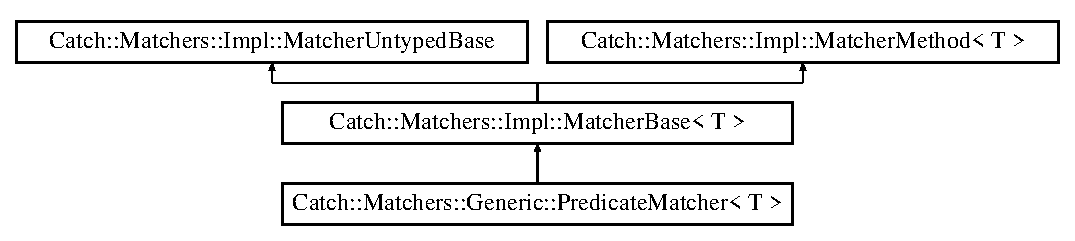
\includegraphics[height=2.790698cm]{class_catch_1_1_matchers_1_1_generic_1_1_predicate_matcher}
\end{center}
\end{figure}
\subsection*{Public Member Functions}
\begin{DoxyCompactItemize}
\item 
\mbox{\Hypertarget{class_catch_1_1_matchers_1_1_generic_1_1_predicate_matcher_a57d53ef028c2f7b92b016f627f91aa76}\label{class_catch_1_1_matchers_1_1_generic_1_1_predicate_matcher_a57d53ef028c2f7b92b016f627f91aa76}} 
{\bfseries Predicate\+Matcher} (std\+::function$<$ bool(T const \&)$>$ const \&elem, std\+::string const \&descr)
\item 
\mbox{\Hypertarget{class_catch_1_1_matchers_1_1_generic_1_1_predicate_matcher_a2ec0e8ec19c4c5e26271d59a06a62b52}\label{class_catch_1_1_matchers_1_1_generic_1_1_predicate_matcher_a2ec0e8ec19c4c5e26271d59a06a62b52}} 
bool {\bfseries match} (T const \&item) const override
\item 
\mbox{\Hypertarget{class_catch_1_1_matchers_1_1_generic_1_1_predicate_matcher_af7d59e94892cc09471bbaefac4c889fd}\label{class_catch_1_1_matchers_1_1_generic_1_1_predicate_matcher_af7d59e94892cc09471bbaefac4c889fd}} 
std\+::string {\bfseries describe} () const override
\end{DoxyCompactItemize}
\subsection*{Additional Inherited Members}


The documentation for this class was generated from the following file\+:\begin{DoxyCompactItemize}
\item 
D\+:/kouluhommat/\+Advanced Object-\/\+Oriented Programming/lopputyö/\+Battleship/\+Battleship/catch.\+hpp\end{DoxyCompactItemize}

\hypertarget{class_catch_1_1_generators_1_1_range_generator}{}\section{Catch\+:\+:Generators\+:\+:Range\+Generator$<$ T $>$ Class Template Reference}
\label{class_catch_1_1_generators_1_1_range_generator}\index{Catch\+::\+Generators\+::\+Range\+Generator$<$ T $>$@{Catch\+::\+Generators\+::\+Range\+Generator$<$ T $>$}}


{\ttfamily \#include $<$catch.\+hpp$>$}

Inheritance diagram for Catch\+:\+:Generators\+:\+:Range\+Generator$<$ T $>$\+:\begin{figure}[H]
\begin{center}
\leavevmode
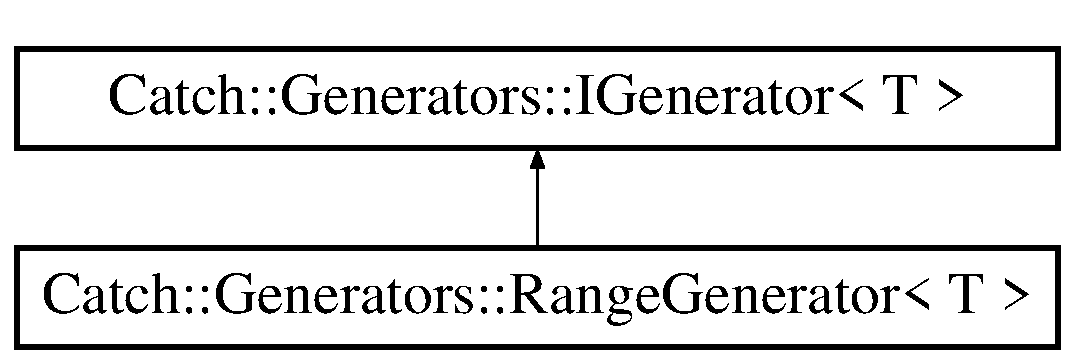
\includegraphics[height=2.000000cm]{class_catch_1_1_generators_1_1_range_generator}
\end{center}
\end{figure}
\subsection*{Public Member Functions}
\begin{DoxyCompactItemize}
\item 
\mbox{\hyperlink{class_catch_1_1_generators_1_1_range_generator_a56c5fcc855bdb668d7b93c2017a7c44c}{Range\+Generator}} (T const \&first, T const \&last)
\item 
auto \mbox{\hyperlink{class_catch_1_1_generators_1_1_range_generator_a78f7f624b7545823d1a683ebf2ac00e7}{get}} (size\+\_\+t index) const -\/$>$ T override
\end{DoxyCompactItemize}


\subsection{Constructor \& Destructor Documentation}
\mbox{\Hypertarget{class_catch_1_1_generators_1_1_range_generator_a56c5fcc855bdb668d7b93c2017a7c44c}\label{class_catch_1_1_generators_1_1_range_generator_a56c5fcc855bdb668d7b93c2017a7c44c}} 
\index{Catch\+::\+Generators\+::\+Range\+Generator@{Catch\+::\+Generators\+::\+Range\+Generator}!Range\+Generator@{Range\+Generator}}
\index{Range\+Generator@{Range\+Generator}!Catch\+::\+Generators\+::\+Range\+Generator@{Catch\+::\+Generators\+::\+Range\+Generator}}
\subsubsection{\texorpdfstring{Range\+Generator()}{RangeGenerator()}}
{\footnotesize\ttfamily template$<$typename T $>$ \\
\mbox{\hyperlink{class_catch_1_1_generators_1_1_range_generator}{Catch\+::\+Generators\+::\+Range\+Generator}}$<$ T $>$\+::\mbox{\hyperlink{class_catch_1_1_generators_1_1_range_generator}{Range\+Generator}} (\begin{DoxyParamCaption}\item[{T const \&}]{first,  }\item[{T const \&}]{last }\end{DoxyParamCaption})\hspace{0.3cm}{\ttfamily [inline]}}



\subsection{Member Function Documentation}
\mbox{\Hypertarget{class_catch_1_1_generators_1_1_range_generator_a78f7f624b7545823d1a683ebf2ac00e7}\label{class_catch_1_1_generators_1_1_range_generator_a78f7f624b7545823d1a683ebf2ac00e7}} 
\index{Catch\+::\+Generators\+::\+Range\+Generator@{Catch\+::\+Generators\+::\+Range\+Generator}!get@{get}}
\index{get@{get}!Catch\+::\+Generators\+::\+Range\+Generator@{Catch\+::\+Generators\+::\+Range\+Generator}}
\subsubsection{\texorpdfstring{get()}{get()}}
{\footnotesize\ttfamily template$<$typename T $>$ \\
auto \mbox{\hyperlink{class_catch_1_1_generators_1_1_range_generator}{Catch\+::\+Generators\+::\+Range\+Generator}}$<$ T $>$\+::get (\begin{DoxyParamCaption}\item[{size\+\_\+t}]{index }\end{DoxyParamCaption}) const -\/$>$ T\hspace{0.3cm}{\ttfamily [inline]}, {\ttfamily [override]}, {\ttfamily [virtual]}}



Implements \mbox{\hyperlink{struct_catch_1_1_generators_1_1_i_generator_a737a89eb0bff02e580e36c59fb0d1171}{Catch\+::\+Generators\+::\+I\+Generator$<$ T $>$}}.



The documentation for this class was generated from the following file\+:\begin{DoxyCompactItemize}
\item 
D\+:/kouluhommat/\+Advanced Object-\/\+Oriented Programming/lopputyö/\+Battleship/\+Battleship/\mbox{\hyperlink{catch_8hpp}{catch.\+hpp}}\end{DoxyCompactItemize}

\hypertarget{struct_catch_1_1_matchers_1_1_std_string_1_1_regex_matcher}{}\section{Catch\+:\+:Matchers\+:\+:Std\+String\+:\+:Regex\+Matcher Struct Reference}
\label{struct_catch_1_1_matchers_1_1_std_string_1_1_regex_matcher}\index{Catch\+::\+Matchers\+::\+Std\+String\+::\+Regex\+Matcher@{Catch\+::\+Matchers\+::\+Std\+String\+::\+Regex\+Matcher}}


{\ttfamily \#include $<$catch.\+hpp$>$}

Inheritance diagram for Catch\+:\+:Matchers\+:\+:Std\+String\+:\+:Regex\+Matcher\+:\begin{figure}[H]
\begin{center}
\leavevmode
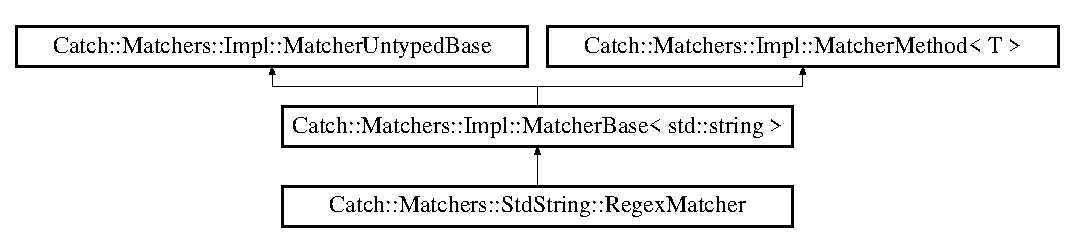
\includegraphics[height=2.818792cm]{struct_catch_1_1_matchers_1_1_std_string_1_1_regex_matcher}
\end{center}
\end{figure}
\subsection*{Public Member Functions}
\begin{DoxyCompactItemize}
\item 
\mbox{\hyperlink{struct_catch_1_1_matchers_1_1_std_string_1_1_regex_matcher_ab914deb885fe25558c41ab368c6b3916}{Regex\+Matcher}} (std\+::string regex, \mbox{\hyperlink{struct_catch_1_1_case_sensitive_aad49d3aee2d97066642fffa919685c6a}{Case\+Sensitive\+::\+Choice}} case\+Sensitivity)
\item 
bool \mbox{\hyperlink{struct_catch_1_1_matchers_1_1_std_string_1_1_regex_matcher_aa8e61adccabb2f36133029301f6b8f4e}{match}} (std\+::string const \&matchee) const override
\item 
std\+::string \mbox{\hyperlink{struct_catch_1_1_matchers_1_1_std_string_1_1_regex_matcher_a1f788cd5258c987e5043f6c7f43adeb9}{describe}} () const override
\end{DoxyCompactItemize}
\subsection*{Additional Inherited Members}


\subsection{Constructor \& Destructor Documentation}
\mbox{\Hypertarget{struct_catch_1_1_matchers_1_1_std_string_1_1_regex_matcher_ab914deb885fe25558c41ab368c6b3916}\label{struct_catch_1_1_matchers_1_1_std_string_1_1_regex_matcher_ab914deb885fe25558c41ab368c6b3916}} 
\index{Catch\+::\+Matchers\+::\+Std\+String\+::\+Regex\+Matcher@{Catch\+::\+Matchers\+::\+Std\+String\+::\+Regex\+Matcher}!Regex\+Matcher@{Regex\+Matcher}}
\index{Regex\+Matcher@{Regex\+Matcher}!Catch\+::\+Matchers\+::\+Std\+String\+::\+Regex\+Matcher@{Catch\+::\+Matchers\+::\+Std\+String\+::\+Regex\+Matcher}}
\subsubsection{\texorpdfstring{Regex\+Matcher()}{RegexMatcher()}}
{\footnotesize\ttfamily Catch\+::\+Matchers\+::\+Std\+String\+::\+Regex\+Matcher\+::\+Regex\+Matcher (\begin{DoxyParamCaption}\item[{std\+::string}]{regex,  }\item[{\mbox{\hyperlink{struct_catch_1_1_case_sensitive_aad49d3aee2d97066642fffa919685c6a}{Case\+Sensitive\+::\+Choice}}}]{case\+Sensitivity }\end{DoxyParamCaption})}



\subsection{Member Function Documentation}
\mbox{\Hypertarget{struct_catch_1_1_matchers_1_1_std_string_1_1_regex_matcher_a1f788cd5258c987e5043f6c7f43adeb9}\label{struct_catch_1_1_matchers_1_1_std_string_1_1_regex_matcher_a1f788cd5258c987e5043f6c7f43adeb9}} 
\index{Catch\+::\+Matchers\+::\+Std\+String\+::\+Regex\+Matcher@{Catch\+::\+Matchers\+::\+Std\+String\+::\+Regex\+Matcher}!describe@{describe}}
\index{describe@{describe}!Catch\+::\+Matchers\+::\+Std\+String\+::\+Regex\+Matcher@{Catch\+::\+Matchers\+::\+Std\+String\+::\+Regex\+Matcher}}
\subsubsection{\texorpdfstring{describe()}{describe()}}
{\footnotesize\ttfamily std\+::string Catch\+::\+Matchers\+::\+Std\+String\+::\+Regex\+Matcher\+::describe (\begin{DoxyParamCaption}{ }\end{DoxyParamCaption}) const\hspace{0.3cm}{\ttfamily [override]}, {\ttfamily [virtual]}}



Implements \mbox{\hyperlink{class_catch_1_1_matchers_1_1_impl_1_1_matcher_untyped_base_a91d3a907dbfcbb596077df24f6e11fe2}{Catch\+::\+Matchers\+::\+Impl\+::\+Matcher\+Untyped\+Base}}.

\mbox{\Hypertarget{struct_catch_1_1_matchers_1_1_std_string_1_1_regex_matcher_aa8e61adccabb2f36133029301f6b8f4e}\label{struct_catch_1_1_matchers_1_1_std_string_1_1_regex_matcher_aa8e61adccabb2f36133029301f6b8f4e}} 
\index{Catch\+::\+Matchers\+::\+Std\+String\+::\+Regex\+Matcher@{Catch\+::\+Matchers\+::\+Std\+String\+::\+Regex\+Matcher}!match@{match}}
\index{match@{match}!Catch\+::\+Matchers\+::\+Std\+String\+::\+Regex\+Matcher@{Catch\+::\+Matchers\+::\+Std\+String\+::\+Regex\+Matcher}}
\subsubsection{\texorpdfstring{match()}{match()}}
{\footnotesize\ttfamily bool Catch\+::\+Matchers\+::\+Std\+String\+::\+Regex\+Matcher\+::match (\begin{DoxyParamCaption}\item[{std\+::string const \&}]{matchee }\end{DoxyParamCaption}) const\hspace{0.3cm}{\ttfamily [override]}}



The documentation for this struct was generated from the following file\+:\begin{DoxyCompactItemize}
\item 
D\+:/kouluhommat/\+Advanced Object-\/\+Oriented Programming/lopputyö/\+Battleship/\+Battleship/\mbox{\hyperlink{catch_8hpp}{catch.\+hpp}}\end{DoxyCompactItemize}

\hypertarget{struct_catch_1_1_registrar_for_tag_aliases}{}\section{Catch\+:\+:Registrar\+For\+Tag\+Aliases Struct Reference}
\label{struct_catch_1_1_registrar_for_tag_aliases}\index{Catch\+::\+Registrar\+For\+Tag\+Aliases@{Catch\+::\+Registrar\+For\+Tag\+Aliases}}


{\ttfamily \#include $<$catch.\+hpp$>$}

\subsection*{Public Member Functions}
\begin{DoxyCompactItemize}
\item 
\mbox{\hyperlink{struct_catch_1_1_registrar_for_tag_aliases_ae4e45830e4763bcd65d55d8db9167b69}{Registrar\+For\+Tag\+Aliases}} (char const $\ast$alias, char const $\ast$tag, \mbox{\hyperlink{struct_catch_1_1_source_line_info}{Source\+Line\+Info}} const \&line\+Info)
\end{DoxyCompactItemize}


\subsection{Constructor \& Destructor Documentation}
\mbox{\Hypertarget{struct_catch_1_1_registrar_for_tag_aliases_ae4e45830e4763bcd65d55d8db9167b69}\label{struct_catch_1_1_registrar_for_tag_aliases_ae4e45830e4763bcd65d55d8db9167b69}} 
\index{Catch\+::\+Registrar\+For\+Tag\+Aliases@{Catch\+::\+Registrar\+For\+Tag\+Aliases}!Registrar\+For\+Tag\+Aliases@{Registrar\+For\+Tag\+Aliases}}
\index{Registrar\+For\+Tag\+Aliases@{Registrar\+For\+Tag\+Aliases}!Catch\+::\+Registrar\+For\+Tag\+Aliases@{Catch\+::\+Registrar\+For\+Tag\+Aliases}}
\subsubsection{\texorpdfstring{Registrar\+For\+Tag\+Aliases()}{RegistrarForTagAliases()}}
{\footnotesize\ttfamily Catch\+::\+Registrar\+For\+Tag\+Aliases\+::\+Registrar\+For\+Tag\+Aliases (\begin{DoxyParamCaption}\item[{char const $\ast$}]{alias,  }\item[{char const $\ast$}]{tag,  }\item[{\mbox{\hyperlink{struct_catch_1_1_source_line_info}{Source\+Line\+Info}} const \&}]{line\+Info }\end{DoxyParamCaption})}



The documentation for this struct was generated from the following file\+:\begin{DoxyCompactItemize}
\item 
D\+:/kouluhommat/\+Advanced Object-\/\+Oriented Programming/lopputyö/\+Battleship/\+Battleship/\mbox{\hyperlink{catch_8hpp}{catch.\+hpp}}\end{DoxyCompactItemize}

\hypertarget{struct_catch_1_1_generators_1_1_requires_a_specialisation_for}{}\section{Catch\+:\+:Generators\+:\+:Requires\+A\+Specialisation\+For$<$ T $>$ Struct Template Reference}
\label{struct_catch_1_1_generators_1_1_requires_a_specialisation_for}\index{Catch\+::\+Generators\+::\+Requires\+A\+Specialisation\+For$<$ T $>$@{Catch\+::\+Generators\+::\+Requires\+A\+Specialisation\+For$<$ T $>$}}


The documentation for this struct was generated from the following file\+:\begin{DoxyCompactItemize}
\item 
D\+:/kouluhommat/\+Advanced Object-\/\+Oriented Programming/lopputyö/\+Battleship/\+Battleship/catch.\+hpp\end{DoxyCompactItemize}

\hypertarget{struct_catch_1_1_result_disposition}{}\section{Catch\+:\+:Result\+Disposition Struct Reference}
\label{struct_catch_1_1_result_disposition}\index{Catch\+::\+Result\+Disposition@{Catch\+::\+Result\+Disposition}}


{\ttfamily \#include $<$catch.\+hpp$>$}

\subsection*{Public Types}
\begin{DoxyCompactItemize}
\item 
enum \mbox{\hyperlink{struct_catch_1_1_result_disposition_a3396cad6e2259af326b3aae93e23e9d8}{Flags}} \{ \mbox{\hyperlink{struct_catch_1_1_result_disposition_a3396cad6e2259af326b3aae93e23e9d8af3bd52347ed6f8796e8ce2f77bb39ea5}{Normal}} = 0x01, 
\mbox{\hyperlink{struct_catch_1_1_result_disposition_a3396cad6e2259af326b3aae93e23e9d8aa18c94bd60c5614e17a84c2ced3bbfd5}{Continue\+On\+Failure}} = 0x02, 
\mbox{\hyperlink{struct_catch_1_1_result_disposition_a3396cad6e2259af326b3aae93e23e9d8a9980604245f19884691f941dec03eeb8}{False\+Test}} = 0x04, 
\mbox{\hyperlink{struct_catch_1_1_result_disposition_a3396cad6e2259af326b3aae93e23e9d8a1a88eb6004bddee4ccae4b421991bf54}{Suppress\+Fail}} = 0x08
 \}
\end{DoxyCompactItemize}


\subsection{Member Enumeration Documentation}
\mbox{\Hypertarget{struct_catch_1_1_result_disposition_a3396cad6e2259af326b3aae93e23e9d8}\label{struct_catch_1_1_result_disposition_a3396cad6e2259af326b3aae93e23e9d8}} 
\index{Catch\+::\+Result\+Disposition@{Catch\+::\+Result\+Disposition}!Flags@{Flags}}
\index{Flags@{Flags}!Catch\+::\+Result\+Disposition@{Catch\+::\+Result\+Disposition}}
\subsubsection{\texorpdfstring{Flags}{Flags}}
{\footnotesize\ttfamily enum \mbox{\hyperlink{struct_catch_1_1_result_disposition_a3396cad6e2259af326b3aae93e23e9d8}{Catch\+::\+Result\+Disposition\+::\+Flags}}}

\begin{DoxyEnumFields}{Enumerator}
\raisebox{\heightof{T}}[0pt][0pt]{\index{Normal@{Normal}!Catch\+::\+Result\+Disposition@{Catch\+::\+Result\+Disposition}}\index{Catch\+::\+Result\+Disposition@{Catch\+::\+Result\+Disposition}!Normal@{Normal}}}\mbox{\Hypertarget{struct_catch_1_1_result_disposition_a3396cad6e2259af326b3aae93e23e9d8af3bd52347ed6f8796e8ce2f77bb39ea5}\label{struct_catch_1_1_result_disposition_a3396cad6e2259af326b3aae93e23e9d8af3bd52347ed6f8796e8ce2f77bb39ea5}} 
Normal&\\
\hline

\raisebox{\heightof{T}}[0pt][0pt]{\index{Continue\+On\+Failure@{Continue\+On\+Failure}!Catch\+::\+Result\+Disposition@{Catch\+::\+Result\+Disposition}}\index{Catch\+::\+Result\+Disposition@{Catch\+::\+Result\+Disposition}!Continue\+On\+Failure@{Continue\+On\+Failure}}}\mbox{\Hypertarget{struct_catch_1_1_result_disposition_a3396cad6e2259af326b3aae93e23e9d8aa18c94bd60c5614e17a84c2ced3bbfd5}\label{struct_catch_1_1_result_disposition_a3396cad6e2259af326b3aae93e23e9d8aa18c94bd60c5614e17a84c2ced3bbfd5}} 
Continue\+On\+Failure&\\
\hline

\raisebox{\heightof{T}}[0pt][0pt]{\index{False\+Test@{False\+Test}!Catch\+::\+Result\+Disposition@{Catch\+::\+Result\+Disposition}}\index{Catch\+::\+Result\+Disposition@{Catch\+::\+Result\+Disposition}!False\+Test@{False\+Test}}}\mbox{\Hypertarget{struct_catch_1_1_result_disposition_a3396cad6e2259af326b3aae93e23e9d8a9980604245f19884691f941dec03eeb8}\label{struct_catch_1_1_result_disposition_a3396cad6e2259af326b3aae93e23e9d8a9980604245f19884691f941dec03eeb8}} 
False\+Test&\\
\hline

\raisebox{\heightof{T}}[0pt][0pt]{\index{Suppress\+Fail@{Suppress\+Fail}!Catch\+::\+Result\+Disposition@{Catch\+::\+Result\+Disposition}}\index{Catch\+::\+Result\+Disposition@{Catch\+::\+Result\+Disposition}!Suppress\+Fail@{Suppress\+Fail}}}\mbox{\Hypertarget{struct_catch_1_1_result_disposition_a3396cad6e2259af326b3aae93e23e9d8a1a88eb6004bddee4ccae4b421991bf54}\label{struct_catch_1_1_result_disposition_a3396cad6e2259af326b3aae93e23e9d8a1a88eb6004bddee4ccae4b421991bf54}} 
Suppress\+Fail&\\
\hline

\end{DoxyEnumFields}


The documentation for this struct was generated from the following file\+:\begin{DoxyCompactItemize}
\item 
D\+:/kouluhommat/\+Advanced Object-\/\+Oriented Programming/lopputyö/\+Battleship/\+Battleship/\mbox{\hyperlink{catch_8hpp}{catch.\+hpp}}\end{DoxyCompactItemize}

\hypertarget{struct_catch_1_1_result_was}{}\section{Catch\+:\+:Result\+Was Struct Reference}
\label{struct_catch_1_1_result_was}\index{Catch\+::\+Result\+Was@{Catch\+::\+Result\+Was}}


{\ttfamily \#include $<$catch.\+hpp$>$}

\subsection*{Public Types}
\begin{DoxyCompactItemize}
\item 
enum \mbox{\hyperlink{struct_catch_1_1_result_was_a624e1ee3661fcf6094ceef1f654601ef}{Of\+Type}} \{ \newline
\mbox{\hyperlink{struct_catch_1_1_result_was_a624e1ee3661fcf6094ceef1f654601efa65721dda02fe5efb522e7449e496608a}{Unknown}} = -\/1, 
\mbox{\hyperlink{struct_catch_1_1_result_was_a624e1ee3661fcf6094ceef1f654601efae7cbe89bb9ec7ece9b44d48b63d01b63}{Ok}} = 0, 
\mbox{\hyperlink{struct_catch_1_1_result_was_a624e1ee3661fcf6094ceef1f654601efa30222063929ca1b6318faa78e8242f1c}{Info}} = 1, 
\mbox{\hyperlink{struct_catch_1_1_result_was_a624e1ee3661fcf6094ceef1f654601efa67e9d36ba0f04a60a19896834d840c21}{Warning}} = 2, 
\newline
\mbox{\hyperlink{struct_catch_1_1_result_was_a624e1ee3661fcf6094ceef1f654601efa1818f1b198f10b5734c405142b22025c}{Failure\+Bit}} = 0x10, 
\mbox{\hyperlink{struct_catch_1_1_result_was_a624e1ee3661fcf6094ceef1f654601efa5e7126b8458dc1376ac870a719f7873f}{Expression\+Failed}} = Failure\+Bit $\vert$ 1, 
\mbox{\hyperlink{struct_catch_1_1_result_was_a624e1ee3661fcf6094ceef1f654601efacecfc052e2499499b13304249303cc36}{Explicit\+Failure}} = Failure\+Bit $\vert$ 2, 
\mbox{\hyperlink{struct_catch_1_1_result_was_a624e1ee3661fcf6094ceef1f654601efaa9107b7836cc7590ca668002f76d27c7}{Exception}} = 0x100 $\vert$ Failure\+Bit, 
\newline
\mbox{\hyperlink{struct_catch_1_1_result_was_a624e1ee3661fcf6094ceef1f654601efa3bb56296483947280cf7fa1ad074ab45}{Threw\+Exception}} = Exception $\vert$ 1, 
\mbox{\hyperlink{struct_catch_1_1_result_was_a624e1ee3661fcf6094ceef1f654601efa8b6d3d5bc78d4e7a95543b6ecfbdb57d}{Didnt\+Throw\+Exception}} = Exception $\vert$ 2, 
\mbox{\hyperlink{struct_catch_1_1_result_was_a624e1ee3661fcf6094ceef1f654601efa87fa1f2a2a63290b61948002e2935377}{Fatal\+Error\+Condition}} = 0x200 $\vert$ Failure\+Bit
 \}
\end{DoxyCompactItemize}


\subsection{Member Enumeration Documentation}
\mbox{\Hypertarget{struct_catch_1_1_result_was_a624e1ee3661fcf6094ceef1f654601ef}\label{struct_catch_1_1_result_was_a624e1ee3661fcf6094ceef1f654601ef}} 
\index{Catch\+::\+Result\+Was@{Catch\+::\+Result\+Was}!Of\+Type@{Of\+Type}}
\index{Of\+Type@{Of\+Type}!Catch\+::\+Result\+Was@{Catch\+::\+Result\+Was}}
\subsubsection{\texorpdfstring{Of\+Type}{OfType}}
{\footnotesize\ttfamily enum \mbox{\hyperlink{struct_catch_1_1_result_was_a624e1ee3661fcf6094ceef1f654601ef}{Catch\+::\+Result\+Was\+::\+Of\+Type}}}

\begin{DoxyEnumFields}{Enumerator}
\raisebox{\heightof{T}}[0pt][0pt]{\index{Unknown@{Unknown}!Catch\+::\+Result\+Was@{Catch\+::\+Result\+Was}}\index{Catch\+::\+Result\+Was@{Catch\+::\+Result\+Was}!Unknown@{Unknown}}}\mbox{\Hypertarget{struct_catch_1_1_result_was_a624e1ee3661fcf6094ceef1f654601efa65721dda02fe5efb522e7449e496608a}\label{struct_catch_1_1_result_was_a624e1ee3661fcf6094ceef1f654601efa65721dda02fe5efb522e7449e496608a}} 
Unknown&\\
\hline

\raisebox{\heightof{T}}[0pt][0pt]{\index{Ok@{Ok}!Catch\+::\+Result\+Was@{Catch\+::\+Result\+Was}}\index{Catch\+::\+Result\+Was@{Catch\+::\+Result\+Was}!Ok@{Ok}}}\mbox{\Hypertarget{struct_catch_1_1_result_was_a624e1ee3661fcf6094ceef1f654601efae7cbe89bb9ec7ece9b44d48b63d01b63}\label{struct_catch_1_1_result_was_a624e1ee3661fcf6094ceef1f654601efae7cbe89bb9ec7ece9b44d48b63d01b63}} 
Ok&\\
\hline

\raisebox{\heightof{T}}[0pt][0pt]{\index{Info@{Info}!Catch\+::\+Result\+Was@{Catch\+::\+Result\+Was}}\index{Catch\+::\+Result\+Was@{Catch\+::\+Result\+Was}!Info@{Info}}}\mbox{\Hypertarget{struct_catch_1_1_result_was_a624e1ee3661fcf6094ceef1f654601efa30222063929ca1b6318faa78e8242f1c}\label{struct_catch_1_1_result_was_a624e1ee3661fcf6094ceef1f654601efa30222063929ca1b6318faa78e8242f1c}} 
Info&\\
\hline

\raisebox{\heightof{T}}[0pt][0pt]{\index{Warning@{Warning}!Catch\+::\+Result\+Was@{Catch\+::\+Result\+Was}}\index{Catch\+::\+Result\+Was@{Catch\+::\+Result\+Was}!Warning@{Warning}}}\mbox{\Hypertarget{struct_catch_1_1_result_was_a624e1ee3661fcf6094ceef1f654601efa67e9d36ba0f04a60a19896834d840c21}\label{struct_catch_1_1_result_was_a624e1ee3661fcf6094ceef1f654601efa67e9d36ba0f04a60a19896834d840c21}} 
Warning&\\
\hline

\raisebox{\heightof{T}}[0pt][0pt]{\index{Failure\+Bit@{Failure\+Bit}!Catch\+::\+Result\+Was@{Catch\+::\+Result\+Was}}\index{Catch\+::\+Result\+Was@{Catch\+::\+Result\+Was}!Failure\+Bit@{Failure\+Bit}}}\mbox{\Hypertarget{struct_catch_1_1_result_was_a624e1ee3661fcf6094ceef1f654601efa1818f1b198f10b5734c405142b22025c}\label{struct_catch_1_1_result_was_a624e1ee3661fcf6094ceef1f654601efa1818f1b198f10b5734c405142b22025c}} 
Failure\+Bit&\\
\hline

\raisebox{\heightof{T}}[0pt][0pt]{\index{Expression\+Failed@{Expression\+Failed}!Catch\+::\+Result\+Was@{Catch\+::\+Result\+Was}}\index{Catch\+::\+Result\+Was@{Catch\+::\+Result\+Was}!Expression\+Failed@{Expression\+Failed}}}\mbox{\Hypertarget{struct_catch_1_1_result_was_a624e1ee3661fcf6094ceef1f654601efa5e7126b8458dc1376ac870a719f7873f}\label{struct_catch_1_1_result_was_a624e1ee3661fcf6094ceef1f654601efa5e7126b8458dc1376ac870a719f7873f}} 
Expression\+Failed&\\
\hline

\raisebox{\heightof{T}}[0pt][0pt]{\index{Explicit\+Failure@{Explicit\+Failure}!Catch\+::\+Result\+Was@{Catch\+::\+Result\+Was}}\index{Catch\+::\+Result\+Was@{Catch\+::\+Result\+Was}!Explicit\+Failure@{Explicit\+Failure}}}\mbox{\Hypertarget{struct_catch_1_1_result_was_a624e1ee3661fcf6094ceef1f654601efacecfc052e2499499b13304249303cc36}\label{struct_catch_1_1_result_was_a624e1ee3661fcf6094ceef1f654601efacecfc052e2499499b13304249303cc36}} 
Explicit\+Failure&\\
\hline

\raisebox{\heightof{T}}[0pt][0pt]{\index{Exception@{Exception}!Catch\+::\+Result\+Was@{Catch\+::\+Result\+Was}}\index{Catch\+::\+Result\+Was@{Catch\+::\+Result\+Was}!Exception@{Exception}}}\mbox{\Hypertarget{struct_catch_1_1_result_was_a624e1ee3661fcf6094ceef1f654601efaa9107b7836cc7590ca668002f76d27c7}\label{struct_catch_1_1_result_was_a624e1ee3661fcf6094ceef1f654601efaa9107b7836cc7590ca668002f76d27c7}} 
Exception&\\
\hline

\raisebox{\heightof{T}}[0pt][0pt]{\index{Threw\+Exception@{Threw\+Exception}!Catch\+::\+Result\+Was@{Catch\+::\+Result\+Was}}\index{Catch\+::\+Result\+Was@{Catch\+::\+Result\+Was}!Threw\+Exception@{Threw\+Exception}}}\mbox{\Hypertarget{struct_catch_1_1_result_was_a624e1ee3661fcf6094ceef1f654601efa3bb56296483947280cf7fa1ad074ab45}\label{struct_catch_1_1_result_was_a624e1ee3661fcf6094ceef1f654601efa3bb56296483947280cf7fa1ad074ab45}} 
Threw\+Exception&\\
\hline

\raisebox{\heightof{T}}[0pt][0pt]{\index{Didnt\+Throw\+Exception@{Didnt\+Throw\+Exception}!Catch\+::\+Result\+Was@{Catch\+::\+Result\+Was}}\index{Catch\+::\+Result\+Was@{Catch\+::\+Result\+Was}!Didnt\+Throw\+Exception@{Didnt\+Throw\+Exception}}}\mbox{\Hypertarget{struct_catch_1_1_result_was_a624e1ee3661fcf6094ceef1f654601efa8b6d3d5bc78d4e7a95543b6ecfbdb57d}\label{struct_catch_1_1_result_was_a624e1ee3661fcf6094ceef1f654601efa8b6d3d5bc78d4e7a95543b6ecfbdb57d}} 
Didnt\+Throw\+Exception&\\
\hline

\raisebox{\heightof{T}}[0pt][0pt]{\index{Fatal\+Error\+Condition@{Fatal\+Error\+Condition}!Catch\+::\+Result\+Was@{Catch\+::\+Result\+Was}}\index{Catch\+::\+Result\+Was@{Catch\+::\+Result\+Was}!Fatal\+Error\+Condition@{Fatal\+Error\+Condition}}}\mbox{\Hypertarget{struct_catch_1_1_result_was_a624e1ee3661fcf6094ceef1f654601efa87fa1f2a2a63290b61948002e2935377}\label{struct_catch_1_1_result_was_a624e1ee3661fcf6094ceef1f654601efa87fa1f2a2a63290b61948002e2935377}} 
Fatal\+Error\+Condition&\\
\hline

\end{DoxyEnumFields}


The documentation for this struct was generated from the following file\+:\begin{DoxyCompactItemize}
\item 
D\+:/kouluhommat/\+Advanced Object-\/\+Oriented Programming/lopputyö/\+Battleship/\+Battleship/\mbox{\hyperlink{catch_8hpp}{catch.\+hpp}}\end{DoxyCompactItemize}

\hypertarget{class_catch_1_1_reusable_string_stream}{}\section{Catch\+:\+:Reusable\+String\+Stream Class Reference}
\label{class_catch_1_1_reusable_string_stream}\index{Catch\+::\+Reusable\+String\+Stream@{Catch\+::\+Reusable\+String\+Stream}}


{\ttfamily \#include $<$catch.\+hpp$>$}

\subsection*{Public Member Functions}
\begin{DoxyCompactItemize}
\item 
\mbox{\hyperlink{class_catch_1_1_reusable_string_stream_a9b3f8c52b0d2d63ffd825297a9c09781}{Reusable\+String\+Stream}} ()
\item 
\mbox{\hyperlink{class_catch_1_1_reusable_string_stream_aba9384e258a4db3178447b6a58414712}{$\sim$\+Reusable\+String\+Stream}} ()
\item 
auto \mbox{\hyperlink{class_catch_1_1_reusable_string_stream_a0e9ecf260b2a5d35f4886ef0d51f6270}{str}} () const -\/$>$ std\+::string
\item 
{\footnotesize template$<$typename T $>$ }\\auto \mbox{\hyperlink{class_catch_1_1_reusable_string_stream_af95f72024c082db70e5e50782e28e4f6}{operator$<$$<$}} (T const \&value) -\/$>$ \mbox{\hyperlink{class_catch_1_1_reusable_string_stream}{Reusable\+String\+Stream}} \&
\item 
auto \mbox{\hyperlink{class_catch_1_1_reusable_string_stream_a6881808c60a080d4e24a0b81c94cbf67}{get}} () -\/$>$ std\+::ostream \&
\end{DoxyCompactItemize}


\subsection{Constructor \& Destructor Documentation}
\mbox{\Hypertarget{class_catch_1_1_reusable_string_stream_a9b3f8c52b0d2d63ffd825297a9c09781}\label{class_catch_1_1_reusable_string_stream_a9b3f8c52b0d2d63ffd825297a9c09781}} 
\index{Catch\+::\+Reusable\+String\+Stream@{Catch\+::\+Reusable\+String\+Stream}!Reusable\+String\+Stream@{Reusable\+String\+Stream}}
\index{Reusable\+String\+Stream@{Reusable\+String\+Stream}!Catch\+::\+Reusable\+String\+Stream@{Catch\+::\+Reusable\+String\+Stream}}
\subsubsection{\texorpdfstring{Reusable\+String\+Stream()}{ReusableStringStream()}}
{\footnotesize\ttfamily Catch\+::\+Reusable\+String\+Stream\+::\+Reusable\+String\+Stream (\begin{DoxyParamCaption}{ }\end{DoxyParamCaption})}

\mbox{\Hypertarget{class_catch_1_1_reusable_string_stream_aba9384e258a4db3178447b6a58414712}\label{class_catch_1_1_reusable_string_stream_aba9384e258a4db3178447b6a58414712}} 
\index{Catch\+::\+Reusable\+String\+Stream@{Catch\+::\+Reusable\+String\+Stream}!````~Reusable\+String\+Stream@{$\sim$\+Reusable\+String\+Stream}}
\index{````~Reusable\+String\+Stream@{$\sim$\+Reusable\+String\+Stream}!Catch\+::\+Reusable\+String\+Stream@{Catch\+::\+Reusable\+String\+Stream}}
\subsubsection{\texorpdfstring{$\sim$\+Reusable\+String\+Stream()}{~ReusableStringStream()}}
{\footnotesize\ttfamily Catch\+::\+Reusable\+String\+Stream\+::$\sim$\+Reusable\+String\+Stream (\begin{DoxyParamCaption}{ }\end{DoxyParamCaption})}



\subsection{Member Function Documentation}
\mbox{\Hypertarget{class_catch_1_1_reusable_string_stream_a6881808c60a080d4e24a0b81c94cbf67}\label{class_catch_1_1_reusable_string_stream_a6881808c60a080d4e24a0b81c94cbf67}} 
\index{Catch\+::\+Reusable\+String\+Stream@{Catch\+::\+Reusable\+String\+Stream}!get@{get}}
\index{get@{get}!Catch\+::\+Reusable\+String\+Stream@{Catch\+::\+Reusable\+String\+Stream}}
\subsubsection{\texorpdfstring{get()}{get()}}
{\footnotesize\ttfamily auto Catch\+::\+Reusable\+String\+Stream\+::get (\begin{DoxyParamCaption}{ }\end{DoxyParamCaption}) -\/$>$ std\+::ostream\& \hspace{0.3cm}{\ttfamily [inline]}}

\mbox{\Hypertarget{class_catch_1_1_reusable_string_stream_af95f72024c082db70e5e50782e28e4f6}\label{class_catch_1_1_reusable_string_stream_af95f72024c082db70e5e50782e28e4f6}} 
\index{Catch\+::\+Reusable\+String\+Stream@{Catch\+::\+Reusable\+String\+Stream}!operator$<$$<$@{operator$<$$<$}}
\index{operator$<$$<$@{operator$<$$<$}!Catch\+::\+Reusable\+String\+Stream@{Catch\+::\+Reusable\+String\+Stream}}
\subsubsection{\texorpdfstring{operator$<$$<$()}{operator<<()}}
{\footnotesize\ttfamily template$<$typename T $>$ \\
auto Catch\+::\+Reusable\+String\+Stream\+::operator$<$$<$ (\begin{DoxyParamCaption}\item[{T const \&}]{value }\end{DoxyParamCaption}) -\/$>$ \mbox{\hyperlink{class_catch_1_1_reusable_string_stream}{Reusable\+String\+Stream}}\& \hspace{0.3cm}{\ttfamily [inline]}}

\mbox{\Hypertarget{class_catch_1_1_reusable_string_stream_a0e9ecf260b2a5d35f4886ef0d51f6270}\label{class_catch_1_1_reusable_string_stream_a0e9ecf260b2a5d35f4886ef0d51f6270}} 
\index{Catch\+::\+Reusable\+String\+Stream@{Catch\+::\+Reusable\+String\+Stream}!str@{str}}
\index{str@{str}!Catch\+::\+Reusable\+String\+Stream@{Catch\+::\+Reusable\+String\+Stream}}
\subsubsection{\texorpdfstring{str()}{str()}}
{\footnotesize\ttfamily auto Catch\+::\+Reusable\+String\+Stream\+::str (\begin{DoxyParamCaption}{ }\end{DoxyParamCaption}) const -\/$>$  std\+::string}



The documentation for this class was generated from the following file\+:\begin{DoxyCompactItemize}
\item 
D\+:/kouluhommat/\+Advanced Object-\/\+Oriented Programming/lopputyö/\+Battleship/\+Battleship/\mbox{\hyperlink{catch_8hpp}{catch.\+hpp}}\end{DoxyCompactItemize}

\hypertarget{class_catch_1_1_scoped_message}{}\section{Catch\+:\+:Scoped\+Message Class Reference}
\label{class_catch_1_1_scoped_message}\index{Catch\+::\+Scoped\+Message@{Catch\+::\+Scoped\+Message}}


{\ttfamily \#include $<$catch.\+hpp$>$}

\subsection*{Public Member Functions}
\begin{DoxyCompactItemize}
\item 
\mbox{\hyperlink{class_catch_1_1_scoped_message_a5cc59f0f2ebe840e6607f83004d49a17}{Scoped\+Message}} (\mbox{\hyperlink{struct_catch_1_1_message_builder}{Message\+Builder}} const \&builder)
\item 
\mbox{\hyperlink{class_catch_1_1_scoped_message_a43190843f9eeb84a0b42b0bc95fdf93a}{$\sim$\+Scoped\+Message}} ()
\end{DoxyCompactItemize}
\subsection*{Public Attributes}
\begin{DoxyCompactItemize}
\item 
\mbox{\hyperlink{struct_catch_1_1_message_info}{Message\+Info}} \mbox{\hyperlink{class_catch_1_1_scoped_message_ae6e1476f389cc6e1586f033b3747b27b}{m\+\_\+info}}
\end{DoxyCompactItemize}


\subsection{Constructor \& Destructor Documentation}
\mbox{\Hypertarget{class_catch_1_1_scoped_message_a5cc59f0f2ebe840e6607f83004d49a17}\label{class_catch_1_1_scoped_message_a5cc59f0f2ebe840e6607f83004d49a17}} 
\index{Catch\+::\+Scoped\+Message@{Catch\+::\+Scoped\+Message}!Scoped\+Message@{Scoped\+Message}}
\index{Scoped\+Message@{Scoped\+Message}!Catch\+::\+Scoped\+Message@{Catch\+::\+Scoped\+Message}}
\subsubsection{\texorpdfstring{Scoped\+Message()}{ScopedMessage()}}
{\footnotesize\ttfamily Catch\+::\+Scoped\+Message\+::\+Scoped\+Message (\begin{DoxyParamCaption}\item[{\mbox{\hyperlink{struct_catch_1_1_message_builder}{Message\+Builder}} const \&}]{builder }\end{DoxyParamCaption})\hspace{0.3cm}{\ttfamily [explicit]}}

\mbox{\Hypertarget{class_catch_1_1_scoped_message_a43190843f9eeb84a0b42b0bc95fdf93a}\label{class_catch_1_1_scoped_message_a43190843f9eeb84a0b42b0bc95fdf93a}} 
\index{Catch\+::\+Scoped\+Message@{Catch\+::\+Scoped\+Message}!````~Scoped\+Message@{$\sim$\+Scoped\+Message}}
\index{````~Scoped\+Message@{$\sim$\+Scoped\+Message}!Catch\+::\+Scoped\+Message@{Catch\+::\+Scoped\+Message}}
\subsubsection{\texorpdfstring{$\sim$\+Scoped\+Message()}{~ScopedMessage()}}
{\footnotesize\ttfamily Catch\+::\+Scoped\+Message\+::$\sim$\+Scoped\+Message (\begin{DoxyParamCaption}{ }\end{DoxyParamCaption})}



\subsection{Member Data Documentation}
\mbox{\Hypertarget{class_catch_1_1_scoped_message_ae6e1476f389cc6e1586f033b3747b27b}\label{class_catch_1_1_scoped_message_ae6e1476f389cc6e1586f033b3747b27b}} 
\index{Catch\+::\+Scoped\+Message@{Catch\+::\+Scoped\+Message}!m\+\_\+info@{m\+\_\+info}}
\index{m\+\_\+info@{m\+\_\+info}!Catch\+::\+Scoped\+Message@{Catch\+::\+Scoped\+Message}}
\subsubsection{\texorpdfstring{m\+\_\+info}{m\_info}}
{\footnotesize\ttfamily \mbox{\hyperlink{struct_catch_1_1_message_info}{Message\+Info}} Catch\+::\+Scoped\+Message\+::m\+\_\+info}



The documentation for this class was generated from the following file\+:\begin{DoxyCompactItemize}
\item 
D\+:/kouluhommat/\+Advanced Object-\/\+Oriented Programming/lopputyö/\+Battleship/\+Battleship/\mbox{\hyperlink{catch_8hpp}{catch.\+hpp}}\end{DoxyCompactItemize}

\hypertarget{class_catch_1_1_section}{}\section{Catch\+:\+:Section Class Reference}
\label{class_catch_1_1_section}\index{Catch\+::\+Section@{Catch\+::\+Section}}
Inheritance diagram for Catch\+:\+:Section\+:\begin{figure}[H]
\begin{center}
\leavevmode
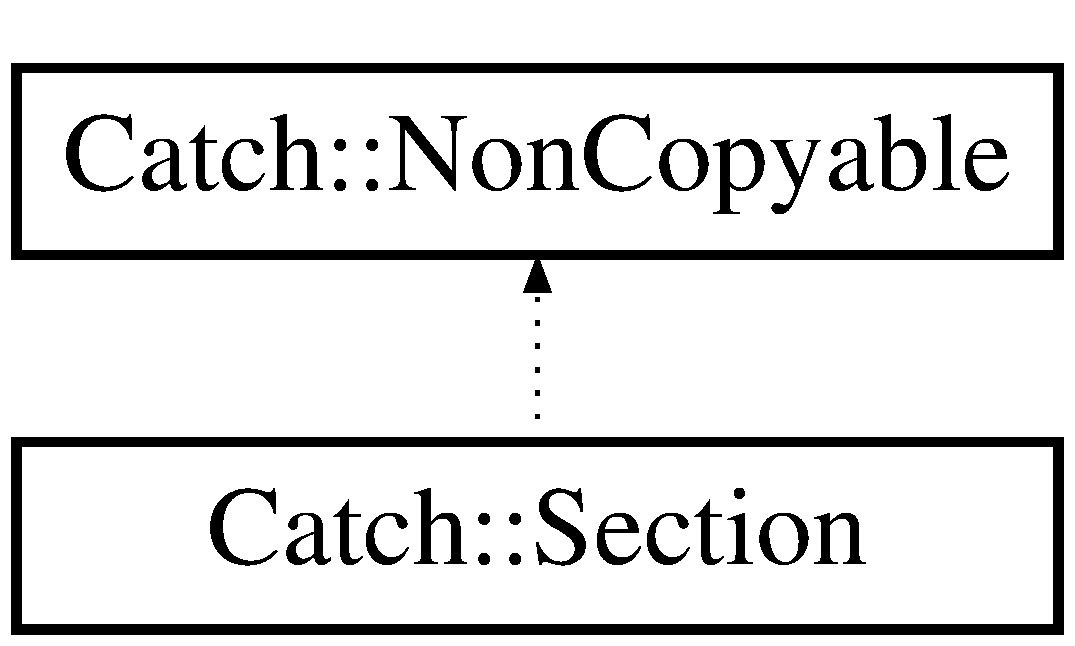
\includegraphics[height=2.000000cm]{class_catch_1_1_section}
\end{center}
\end{figure}
\subsection*{Public Member Functions}
\begin{DoxyCompactItemize}
\item 
\mbox{\Hypertarget{class_catch_1_1_section_a68fd4e51e8981aaa7ddb00d8a6abd099}\label{class_catch_1_1_section_a68fd4e51e8981aaa7ddb00d8a6abd099}} 
{\bfseries Section} (\mbox{\hyperlink{struct_catch_1_1_section_info}{Section\+Info}} const \&info)
\item 
\mbox{\Hypertarget{class_catch_1_1_section_a0632b804dcea1417a2970620a9742eb3}\label{class_catch_1_1_section_a0632b804dcea1417a2970620a9742eb3}} 
{\bfseries operator bool} () const
\end{DoxyCompactItemize}


The documentation for this class was generated from the following file\+:\begin{DoxyCompactItemize}
\item 
D\+:/kouluhommat/\+Advanced Object-\/\+Oriented Programming/lopputyö/\+Battleship/\+Battleship/catch.\+hpp\end{DoxyCompactItemize}

\hypertarget{struct_catch_1_1_section_end_info}{}\section{Catch\+:\+:Section\+End\+Info Struct Reference}
\label{struct_catch_1_1_section_end_info}\index{Catch\+::\+Section\+End\+Info@{Catch\+::\+Section\+End\+Info}}


{\ttfamily \#include $<$catch.\+hpp$>$}

\subsection*{Public Attributes}
\begin{DoxyCompactItemize}
\item 
\mbox{\hyperlink{struct_catch_1_1_section_info}{Section\+Info}} \mbox{\hyperlink{struct_catch_1_1_section_end_info_a2d44793392cb83735d086d726822abe9}{section\+Info}}
\item 
\mbox{\hyperlink{struct_catch_1_1_counts}{Counts}} \mbox{\hyperlink{struct_catch_1_1_section_end_info_ae70b154cbc05b5dd2901d97f89303d8c}{prev\+Assertions}}
\item 
double \mbox{\hyperlink{struct_catch_1_1_section_end_info_a7c262f2dab9cff166b8eca620c47eea5}{duration\+In\+Seconds}}
\end{DoxyCompactItemize}


\subsection{Member Data Documentation}
\mbox{\Hypertarget{struct_catch_1_1_section_end_info_a7c262f2dab9cff166b8eca620c47eea5}\label{struct_catch_1_1_section_end_info_a7c262f2dab9cff166b8eca620c47eea5}} 
\index{Catch\+::\+Section\+End\+Info@{Catch\+::\+Section\+End\+Info}!duration\+In\+Seconds@{duration\+In\+Seconds}}
\index{duration\+In\+Seconds@{duration\+In\+Seconds}!Catch\+::\+Section\+End\+Info@{Catch\+::\+Section\+End\+Info}}
\subsubsection{\texorpdfstring{duration\+In\+Seconds}{durationInSeconds}}
{\footnotesize\ttfamily double Catch\+::\+Section\+End\+Info\+::duration\+In\+Seconds}

\mbox{\Hypertarget{struct_catch_1_1_section_end_info_ae70b154cbc05b5dd2901d97f89303d8c}\label{struct_catch_1_1_section_end_info_ae70b154cbc05b5dd2901d97f89303d8c}} 
\index{Catch\+::\+Section\+End\+Info@{Catch\+::\+Section\+End\+Info}!prev\+Assertions@{prev\+Assertions}}
\index{prev\+Assertions@{prev\+Assertions}!Catch\+::\+Section\+End\+Info@{Catch\+::\+Section\+End\+Info}}
\subsubsection{\texorpdfstring{prev\+Assertions}{prevAssertions}}
{\footnotesize\ttfamily \mbox{\hyperlink{struct_catch_1_1_counts}{Counts}} Catch\+::\+Section\+End\+Info\+::prev\+Assertions}

\mbox{\Hypertarget{struct_catch_1_1_section_end_info_a2d44793392cb83735d086d726822abe9}\label{struct_catch_1_1_section_end_info_a2d44793392cb83735d086d726822abe9}} 
\index{Catch\+::\+Section\+End\+Info@{Catch\+::\+Section\+End\+Info}!section\+Info@{section\+Info}}
\index{section\+Info@{section\+Info}!Catch\+::\+Section\+End\+Info@{Catch\+::\+Section\+End\+Info}}
\subsubsection{\texorpdfstring{section\+Info}{sectionInfo}}
{\footnotesize\ttfamily \mbox{\hyperlink{struct_catch_1_1_section_info}{Section\+Info}} Catch\+::\+Section\+End\+Info\+::section\+Info}



The documentation for this struct was generated from the following file\+:\begin{DoxyCompactItemize}
\item 
D\+:/kouluhommat/\+Advanced Object-\/\+Oriented Programming/lopputyö/\+Battleship/\+Battleship/\mbox{\hyperlink{catch_8hpp}{catch.\+hpp}}\end{DoxyCompactItemize}

\hypertarget{struct_catch_1_1_section_info}{}\section{Catch\+:\+:Section\+Info Struct Reference}
\label{struct_catch_1_1_section_info}\index{Catch\+::\+Section\+Info@{Catch\+::\+Section\+Info}}


{\ttfamily \#include $<$catch.\+hpp$>$}

\subsection*{Public Member Functions}
\begin{DoxyCompactItemize}
\item 
\mbox{\hyperlink{struct_catch_1_1_section_info_a2808437ae7d4bc0830cee1c3995165a6}{Section\+Info}} (\mbox{\hyperlink{struct_catch_1_1_source_line_info}{Source\+Line\+Info}} const \&\+\_\+line\+Info, std\+::string const \&\+\_\+name)
\item 
\mbox{\hyperlink{struct_catch_1_1_section_info_a139875f2e7bd12a5898a948f8bad15b3}{Section\+Info}} (\mbox{\hyperlink{struct_catch_1_1_source_line_info}{Source\+Line\+Info}} const \&\+\_\+line\+Info, std\+::string const \&\+\_\+name, std\+::string const \&)
\end{DoxyCompactItemize}
\subsection*{Public Attributes}
\begin{DoxyCompactItemize}
\item 
std\+::string \mbox{\hyperlink{struct_catch_1_1_section_info_a704c8fc662d309137e0d4f199cb7df58}{name}}
\item 
std\+::string \mbox{\hyperlink{struct_catch_1_1_section_info_a0052060219a6de74bb7ade34d4163a4e}{description}}
\item 
\mbox{\hyperlink{struct_catch_1_1_source_line_info}{Source\+Line\+Info}} \mbox{\hyperlink{struct_catch_1_1_section_info_adbc83b8a3507c4acc8ee249e93465711}{line\+Info}}
\end{DoxyCompactItemize}


\subsection{Constructor \& Destructor Documentation}
\mbox{\Hypertarget{struct_catch_1_1_section_info_a2808437ae7d4bc0830cee1c3995165a6}\label{struct_catch_1_1_section_info_a2808437ae7d4bc0830cee1c3995165a6}} 
\index{Catch\+::\+Section\+Info@{Catch\+::\+Section\+Info}!Section\+Info@{Section\+Info}}
\index{Section\+Info@{Section\+Info}!Catch\+::\+Section\+Info@{Catch\+::\+Section\+Info}}
\subsubsection{\texorpdfstring{Section\+Info()}{SectionInfo()}\hspace{0.1cm}{\footnotesize\ttfamily [1/2]}}
{\footnotesize\ttfamily Catch\+::\+Section\+Info\+::\+Section\+Info (\begin{DoxyParamCaption}\item[{\mbox{\hyperlink{struct_catch_1_1_source_line_info}{Source\+Line\+Info}} const \&}]{\+\_\+line\+Info,  }\item[{std\+::string const \&}]{\+\_\+name }\end{DoxyParamCaption})}

\mbox{\Hypertarget{struct_catch_1_1_section_info_a139875f2e7bd12a5898a948f8bad15b3}\label{struct_catch_1_1_section_info_a139875f2e7bd12a5898a948f8bad15b3}} 
\index{Catch\+::\+Section\+Info@{Catch\+::\+Section\+Info}!Section\+Info@{Section\+Info}}
\index{Section\+Info@{Section\+Info}!Catch\+::\+Section\+Info@{Catch\+::\+Section\+Info}}
\subsubsection{\texorpdfstring{Section\+Info()}{SectionInfo()}\hspace{0.1cm}{\footnotesize\ttfamily [2/2]}}
{\footnotesize\ttfamily Catch\+::\+Section\+Info\+::\+Section\+Info (\begin{DoxyParamCaption}\item[{\mbox{\hyperlink{struct_catch_1_1_source_line_info}{Source\+Line\+Info}} const \&}]{\+\_\+line\+Info,  }\item[{std\+::string const \&}]{\+\_\+name,  }\item[{std\+::string const \&}]{ }\end{DoxyParamCaption})\hspace{0.3cm}{\ttfamily [inline]}}



\subsection{Member Data Documentation}
\mbox{\Hypertarget{struct_catch_1_1_section_info_a0052060219a6de74bb7ade34d4163a4e}\label{struct_catch_1_1_section_info_a0052060219a6de74bb7ade34d4163a4e}} 
\index{Catch\+::\+Section\+Info@{Catch\+::\+Section\+Info}!description@{description}}
\index{description@{description}!Catch\+::\+Section\+Info@{Catch\+::\+Section\+Info}}
\subsubsection{\texorpdfstring{description}{description}}
{\footnotesize\ttfamily std\+::string Catch\+::\+Section\+Info\+::description}

\mbox{\Hypertarget{struct_catch_1_1_section_info_adbc83b8a3507c4acc8ee249e93465711}\label{struct_catch_1_1_section_info_adbc83b8a3507c4acc8ee249e93465711}} 
\index{Catch\+::\+Section\+Info@{Catch\+::\+Section\+Info}!line\+Info@{line\+Info}}
\index{line\+Info@{line\+Info}!Catch\+::\+Section\+Info@{Catch\+::\+Section\+Info}}
\subsubsection{\texorpdfstring{line\+Info}{lineInfo}}
{\footnotesize\ttfamily \mbox{\hyperlink{struct_catch_1_1_source_line_info}{Source\+Line\+Info}} Catch\+::\+Section\+Info\+::line\+Info}

\mbox{\Hypertarget{struct_catch_1_1_section_info_a704c8fc662d309137e0d4f199cb7df58}\label{struct_catch_1_1_section_info_a704c8fc662d309137e0d4f199cb7df58}} 
\index{Catch\+::\+Section\+Info@{Catch\+::\+Section\+Info}!name@{name}}
\index{name@{name}!Catch\+::\+Section\+Info@{Catch\+::\+Section\+Info}}
\subsubsection{\texorpdfstring{name}{name}}
{\footnotesize\ttfamily std\+::string Catch\+::\+Section\+Info\+::name}



The documentation for this struct was generated from the following file\+:\begin{DoxyCompactItemize}
\item 
D\+:/kouluhommat/\+Advanced Object-\/\+Oriented Programming/lopputyö/\+Battleship/\+Battleship/\mbox{\hyperlink{catch_8hpp}{catch.\+hpp}}\end{DoxyCompactItemize}

\hypertarget{class_setup}{}\section{Setup Class Reference}
\label{class_setup}\index{Setup@{Setup}}


{\ttfamily \#include $<$Setup.\+h$>$}

\subsection*{Public Member Functions}
\begin{DoxyCompactItemize}
\item 
\mbox{\hyperlink{class_setup_a0921e54e5a0200af117192e4c0c845b7}{Setup}} ()
\end{DoxyCompactItemize}


\subsection{Detailed Description}
\mbox{\hyperlink{class_setup}{Setup}} class 

\subsection{Constructor \& Destructor Documentation}
\mbox{\Hypertarget{class_setup_a0921e54e5a0200af117192e4c0c845b7}\label{class_setup_a0921e54e5a0200af117192e4c0c845b7}} 
\index{Setup@{Setup}!Setup@{Setup}}
\index{Setup@{Setup}!Setup@{Setup}}
\subsubsection{\texorpdfstring{Setup()}{Setup()}}
{\footnotesize\ttfamily Setup\+::\+Setup (\begin{DoxyParamCaption}{ }\end{DoxyParamCaption})}

Constructor for setup 

The documentation for this class was generated from the following files\+:\begin{DoxyCompactItemize}
\item 
D\+:/kouluhommat/\+Advanced Object-\/\+Oriented Programming/lopputyö/\+Battleship/\+Battleship/\mbox{\hyperlink{_setup_8h}{Setup.\+h}}\item 
D\+:/kouluhommat/\+Advanced Object-\/\+Oriented Programming/lopputyö/\+Battleship/\+Battleship/Setup.\+cpp\end{DoxyCompactItemize}

\hypertarget{class_ship}{}\section{Ship Class Reference}
\label{class_ship}\index{Ship@{Ship}}


{\ttfamily \#include $<$Ship.\+h$>$}

\subsection*{Public Member Functions}
\begin{DoxyCompactItemize}
\item 
\mbox{\hyperlink{class_ship_a1836f4ce3f031b8490a37ac02c5ad65b}{Ship}} (int length, char symbol, std\+::string name, int id)
\begin{DoxyCompactList}\small\item\em Creates \mbox{\hyperlink{class_ship}{Ship}} class. \end{DoxyCompactList}\item 
\mbox{\Hypertarget{class_ship_a5c36a859d4600ba27c091fa9254faadd}\label{class_ship_a5c36a859d4600ba27c091fa9254faadd}} 
int {\bfseries get\+Length} () const
\item 
\mbox{\Hypertarget{class_ship_add61243cfbd60ea5fc3ab79d4ae0c99d}\label{class_ship_add61243cfbd60ea5fc3ab79d4ae0c99d}} 
int \mbox{\hyperlink{class_ship_add61243cfbd60ea5fc3ab79d4ae0c99d}{get\+Ship\+ID}} () const
\begin{DoxyCompactList}\small\item\em Getter for ship\textquotesingle{}s length. \end{DoxyCompactList}\item 
\mbox{\Hypertarget{class_ship_a86ea5893e49e12ceeb6ff43a6f78d86d}\label{class_ship_a86ea5893e49e12ceeb6ff43a6f78d86d}} 
char \mbox{\hyperlink{class_ship_a86ea5893e49e12ceeb6ff43a6f78d86d}{get\+Symbol}} () const
\begin{DoxyCompactList}\small\item\em Getter for ship\textquotesingle{}s ID. \end{DoxyCompactList}\item 
\mbox{\Hypertarget{class_ship_a2ae29387f5c93aa238c3d90526118a20}\label{class_ship_a2ae29387f5c93aa238c3d90526118a20}} 
std\+::string \mbox{\hyperlink{class_ship_a2ae29387f5c93aa238c3d90526118a20}{get\+Name}} () const
\begin{DoxyCompactList}\small\item\em Getter for ship\textquotesingle{}s symbol. \end{DoxyCompactList}\end{DoxyCompactItemize}


\subsection{Detailed Description}
\mbox{\hyperlink{class_ship}{Ship}} class 

\subsection{Constructor \& Destructor Documentation}
\mbox{\Hypertarget{class_ship_a1836f4ce3f031b8490a37ac02c5ad65b}\label{class_ship_a1836f4ce3f031b8490a37ac02c5ad65b}} 
\index{Ship@{Ship}!Ship@{Ship}}
\index{Ship@{Ship}!Ship@{Ship}}
\subsubsection{\texorpdfstring{Ship()}{Ship()}}
{\footnotesize\ttfamily Ship\+::\+Ship (\begin{DoxyParamCaption}\item[{int}]{length,  }\item[{char}]{symbol,  }\item[{std\+::string}]{name,  }\item[{int}]{id }\end{DoxyParamCaption})}



Creates \mbox{\hyperlink{class_ship}{Ship}} class. 

\mbox{\hyperlink{class_ship}{Ship}} constructor 
\begin{DoxyParams}{Parameters}
{\em length} & integer containing ship\textquotesingle{}s length \\
\hline
{\em symbol} & character containing ship\textquotesingle{}s symbol \\
\hline
{\em name} & string containing ship\textquotesingle{}s name \\
\hline
{\em id} & integer containing ship\textquotesingle{}s ID \\
\hline
\end{DoxyParams}


The documentation for this class was generated from the following files\+:\begin{DoxyCompactItemize}
\item 
D\+:/kouluhommat/\+Advanced Object-\/\+Oriented Programming/lopputyö/\+Battleship/\+Battleship/\mbox{\hyperlink{_ship_8h}{Ship.\+h}}\item 
D\+:/kouluhommat/\+Advanced Object-\/\+Oriented Programming/lopputyö/\+Battleship/\+Battleship/\mbox{\hyperlink{_game_8cpp}{Game.\+cpp}}\end{DoxyCompactItemize}

\hypertarget{class_catch_1_1_generators_1_1_single_value_generator}{}\section{Catch\+:\+:Generators\+:\+:Single\+Value\+Generator$<$ T $>$ Class Template Reference}
\label{class_catch_1_1_generators_1_1_single_value_generator}\index{Catch\+::\+Generators\+::\+Single\+Value\+Generator$<$ T $>$@{Catch\+::\+Generators\+::\+Single\+Value\+Generator$<$ T $>$}}


{\ttfamily \#include $<$catch.\+hpp$>$}

Inheritance diagram for Catch\+:\+:Generators\+:\+:Single\+Value\+Generator$<$ T $>$\+:\begin{figure}[H]
\begin{center}
\leavevmode
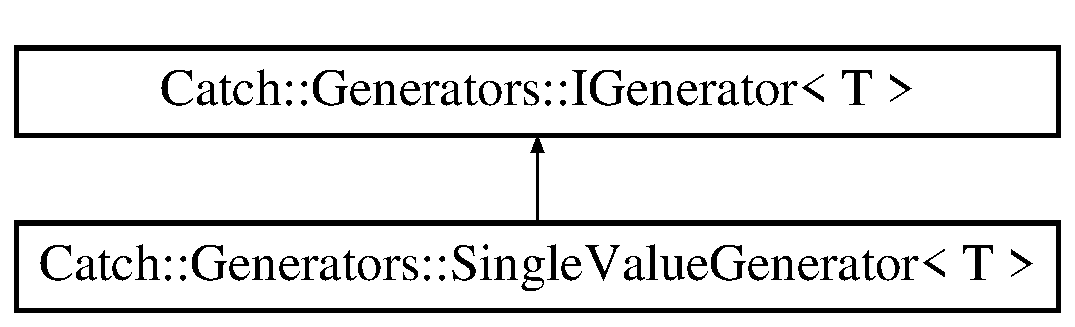
\includegraphics[height=2.000000cm]{class_catch_1_1_generators_1_1_single_value_generator}
\end{center}
\end{figure}
\subsection*{Public Member Functions}
\begin{DoxyCompactItemize}
\item 
\mbox{\hyperlink{class_catch_1_1_generators_1_1_single_value_generator_a4bed2ad14ffe04102d8135e2c82b3ace}{Single\+Value\+Generator}} (T const \&\mbox{\hyperlink{namespace_catch_1_1_generators_a13dbed5ff32f2363862c8ff26661e0ae}{value}})
\item 
auto \mbox{\hyperlink{class_catch_1_1_generators_1_1_single_value_generator_ad03af3fe263136425595bfd2eec84209}{get}} (size\+\_\+t) const -\/$>$ T override
\end{DoxyCompactItemize}


\subsection{Constructor \& Destructor Documentation}
\mbox{\Hypertarget{class_catch_1_1_generators_1_1_single_value_generator_a4bed2ad14ffe04102d8135e2c82b3ace}\label{class_catch_1_1_generators_1_1_single_value_generator_a4bed2ad14ffe04102d8135e2c82b3ace}} 
\index{Catch\+::\+Generators\+::\+Single\+Value\+Generator@{Catch\+::\+Generators\+::\+Single\+Value\+Generator}!Single\+Value\+Generator@{Single\+Value\+Generator}}
\index{Single\+Value\+Generator@{Single\+Value\+Generator}!Catch\+::\+Generators\+::\+Single\+Value\+Generator@{Catch\+::\+Generators\+::\+Single\+Value\+Generator}}
\subsubsection{\texorpdfstring{Single\+Value\+Generator()}{SingleValueGenerator()}}
{\footnotesize\ttfamily template$<$typename T $>$ \\
\mbox{\hyperlink{class_catch_1_1_generators_1_1_single_value_generator}{Catch\+::\+Generators\+::\+Single\+Value\+Generator}}$<$ T $>$\+::\mbox{\hyperlink{class_catch_1_1_generators_1_1_single_value_generator}{Single\+Value\+Generator}} (\begin{DoxyParamCaption}\item[{T const \&}]{value }\end{DoxyParamCaption})\hspace{0.3cm}{\ttfamily [inline]}}



\subsection{Member Function Documentation}
\mbox{\Hypertarget{class_catch_1_1_generators_1_1_single_value_generator_ad03af3fe263136425595bfd2eec84209}\label{class_catch_1_1_generators_1_1_single_value_generator_ad03af3fe263136425595bfd2eec84209}} 
\index{Catch\+::\+Generators\+::\+Single\+Value\+Generator@{Catch\+::\+Generators\+::\+Single\+Value\+Generator}!get@{get}}
\index{get@{get}!Catch\+::\+Generators\+::\+Single\+Value\+Generator@{Catch\+::\+Generators\+::\+Single\+Value\+Generator}}
\subsubsection{\texorpdfstring{get()}{get()}}
{\footnotesize\ttfamily template$<$typename T $>$ \\
auto \mbox{\hyperlink{class_catch_1_1_generators_1_1_single_value_generator}{Catch\+::\+Generators\+::\+Single\+Value\+Generator}}$<$ T $>$\+::get (\begin{DoxyParamCaption}\item[{size\+\_\+t}]{ }\end{DoxyParamCaption}) const -\/$>$ T\hspace{0.3cm}{\ttfamily [inline]}, {\ttfamily [override]}, {\ttfamily [virtual]}}



Implements \mbox{\hyperlink{struct_catch_1_1_generators_1_1_i_generator_a737a89eb0bff02e580e36c59fb0d1171}{Catch\+::\+Generators\+::\+I\+Generator$<$ T $>$}}.



The documentation for this class was generated from the following file\+:\begin{DoxyCompactItemize}
\item 
D\+:/kouluhommat/\+Advanced Object-\/\+Oriented Programming/lopputyö/\+Battleship/\+Battleship/\mbox{\hyperlink{catch_8hpp}{catch.\+hpp}}\end{DoxyCompactItemize}

\hypertarget{struct_catch_1_1_source_line_info}{}\section{Catch\+:\+:Source\+Line\+Info Struct Reference}
\label{struct_catch_1_1_source_line_info}\index{Catch\+::\+Source\+Line\+Info@{Catch\+::\+Source\+Line\+Info}}
\subsection*{Public Member Functions}
\begin{DoxyCompactItemize}
\item 
\mbox{\Hypertarget{struct_catch_1_1_source_line_info_a48510b82a39a042ab370ed143dd30c10}\label{struct_catch_1_1_source_line_info_a48510b82a39a042ab370ed143dd30c10}} 
{\bfseries Source\+Line\+Info} (char const $\ast$\+\_\+file, std\+::size\+\_\+t \+\_\+line) noexcept
\item 
\mbox{\Hypertarget{struct_catch_1_1_source_line_info_a7c44c9986c33a9cf842b791374332d41}\label{struct_catch_1_1_source_line_info_a7c44c9986c33a9cf842b791374332d41}} 
{\bfseries Source\+Line\+Info} (\mbox{\hyperlink{struct_catch_1_1_source_line_info}{Source\+Line\+Info}} const \&other)=default
\item 
\mbox{\Hypertarget{struct_catch_1_1_source_line_info_a6614b503b493bbdd3b49a1bd732e0a55}\label{struct_catch_1_1_source_line_info_a6614b503b493bbdd3b49a1bd732e0a55}} 
{\bfseries Source\+Line\+Info} (\mbox{\hyperlink{struct_catch_1_1_source_line_info}{Source\+Line\+Info}} \&\&)=default
\item 
\mbox{\Hypertarget{struct_catch_1_1_source_line_info_a1a6cfc0197357ef4e329bb256aa8a354}\label{struct_catch_1_1_source_line_info_a1a6cfc0197357ef4e329bb256aa8a354}} 
\mbox{\hyperlink{struct_catch_1_1_source_line_info}{Source\+Line\+Info}} \& {\bfseries operator=} (\mbox{\hyperlink{struct_catch_1_1_source_line_info}{Source\+Line\+Info}} const \&)=default
\item 
\mbox{\Hypertarget{struct_catch_1_1_source_line_info_a7fa35372f2bca5e91adc25327b7c753c}\label{struct_catch_1_1_source_line_info_a7fa35372f2bca5e91adc25327b7c753c}} 
\mbox{\hyperlink{struct_catch_1_1_source_line_info}{Source\+Line\+Info}} \& {\bfseries operator=} (\mbox{\hyperlink{struct_catch_1_1_source_line_info}{Source\+Line\+Info}} \&\&)=default
\item 
\mbox{\Hypertarget{struct_catch_1_1_source_line_info_a10a5b5b7dff82971879c2eb8d83f9b3b}\label{struct_catch_1_1_source_line_info_a10a5b5b7dff82971879c2eb8d83f9b3b}} 
bool {\bfseries empty} () const noexcept
\item 
\mbox{\Hypertarget{struct_catch_1_1_source_line_info_af07e4fdeddf8409b91e4f842f6264cf8}\label{struct_catch_1_1_source_line_info_af07e4fdeddf8409b91e4f842f6264cf8}} 
bool {\bfseries operator==} (\mbox{\hyperlink{struct_catch_1_1_source_line_info}{Source\+Line\+Info}} const \&other) const noexcept
\item 
\mbox{\Hypertarget{struct_catch_1_1_source_line_info_af77415416919d2d6030b4be085b92f7a}\label{struct_catch_1_1_source_line_info_af77415416919d2d6030b4be085b92f7a}} 
bool {\bfseries operator$<$} (\mbox{\hyperlink{struct_catch_1_1_source_line_info}{Source\+Line\+Info}} const \&other) const noexcept
\end{DoxyCompactItemize}
\subsection*{Public Attributes}
\begin{DoxyCompactItemize}
\item 
\mbox{\Hypertarget{struct_catch_1_1_source_line_info_ad65537703e9f08c1fa7777fbc3f0c617}\label{struct_catch_1_1_source_line_info_ad65537703e9f08c1fa7777fbc3f0c617}} 
char const  $\ast$ {\bfseries file}
\item 
\mbox{\Hypertarget{struct_catch_1_1_source_line_info_a841e5d696c7b9cde24e45e61dd979c77}\label{struct_catch_1_1_source_line_info_a841e5d696c7b9cde24e45e61dd979c77}} 
std\+::size\+\_\+t {\bfseries line}
\end{DoxyCompactItemize}


The documentation for this struct was generated from the following file\+:\begin{DoxyCompactItemize}
\item 
D\+:/kouluhommat/\+Advanced Object-\/\+Oriented Programming/lopputyö/\+Battleship/\+Battleship/catch.\+hpp\end{DoxyCompactItemize}

\hypertarget{struct_catch_1_1_matchers_1_1_std_string_1_1_starts_with_matcher}{}\section{Catch\+:\+:Matchers\+:\+:Std\+String\+:\+:Starts\+With\+Matcher Struct Reference}
\label{struct_catch_1_1_matchers_1_1_std_string_1_1_starts_with_matcher}\index{Catch\+::\+Matchers\+::\+Std\+String\+::\+Starts\+With\+Matcher@{Catch\+::\+Matchers\+::\+Std\+String\+::\+Starts\+With\+Matcher}}


{\ttfamily \#include $<$catch.\+hpp$>$}

Inheritance diagram for Catch\+:\+:Matchers\+:\+:Std\+String\+:\+:Starts\+With\+Matcher\+:\begin{figure}[H]
\begin{center}
\leavevmode
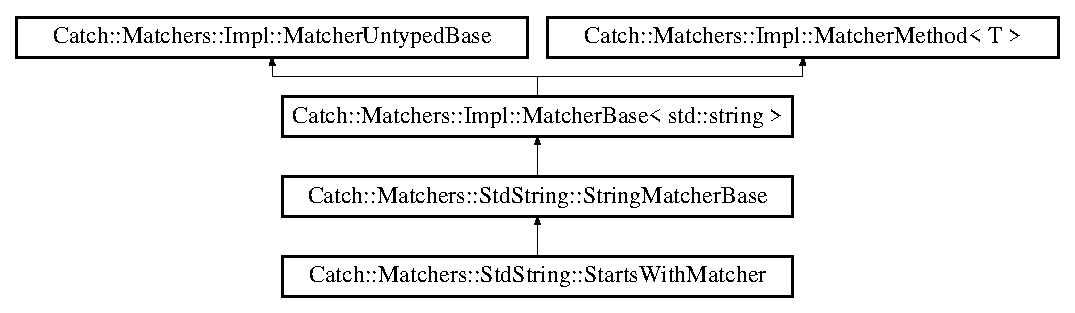
\includegraphics[height=3.758389cm]{struct_catch_1_1_matchers_1_1_std_string_1_1_starts_with_matcher}
\end{center}
\end{figure}
\subsection*{Public Member Functions}
\begin{DoxyCompactItemize}
\item 
\mbox{\hyperlink{struct_catch_1_1_matchers_1_1_std_string_1_1_starts_with_matcher_a7b86f258bdbd131a6e7bcd94a8977325}{Starts\+With\+Matcher}} (\mbox{\hyperlink{struct_catch_1_1_matchers_1_1_std_string_1_1_cased_string}{Cased\+String}} const \&comparator)
\item 
bool \mbox{\hyperlink{struct_catch_1_1_matchers_1_1_std_string_1_1_starts_with_matcher_a7da4747aed0c48989d8be59a89e2b7fb}{match}} (std\+::string const \&source) const override
\end{DoxyCompactItemize}
\subsection*{Additional Inherited Members}


\subsection{Constructor \& Destructor Documentation}
\mbox{\Hypertarget{struct_catch_1_1_matchers_1_1_std_string_1_1_starts_with_matcher_a7b86f258bdbd131a6e7bcd94a8977325}\label{struct_catch_1_1_matchers_1_1_std_string_1_1_starts_with_matcher_a7b86f258bdbd131a6e7bcd94a8977325}} 
\index{Catch\+::\+Matchers\+::\+Std\+String\+::\+Starts\+With\+Matcher@{Catch\+::\+Matchers\+::\+Std\+String\+::\+Starts\+With\+Matcher}!Starts\+With\+Matcher@{Starts\+With\+Matcher}}
\index{Starts\+With\+Matcher@{Starts\+With\+Matcher}!Catch\+::\+Matchers\+::\+Std\+String\+::\+Starts\+With\+Matcher@{Catch\+::\+Matchers\+::\+Std\+String\+::\+Starts\+With\+Matcher}}
\subsubsection{\texorpdfstring{Starts\+With\+Matcher()}{StartsWithMatcher()}}
{\footnotesize\ttfamily Catch\+::\+Matchers\+::\+Std\+String\+::\+Starts\+With\+Matcher\+::\+Starts\+With\+Matcher (\begin{DoxyParamCaption}\item[{\mbox{\hyperlink{struct_catch_1_1_matchers_1_1_std_string_1_1_cased_string}{Cased\+String}} const \&}]{comparator }\end{DoxyParamCaption})}



\subsection{Member Function Documentation}
\mbox{\Hypertarget{struct_catch_1_1_matchers_1_1_std_string_1_1_starts_with_matcher_a7da4747aed0c48989d8be59a89e2b7fb}\label{struct_catch_1_1_matchers_1_1_std_string_1_1_starts_with_matcher_a7da4747aed0c48989d8be59a89e2b7fb}} 
\index{Catch\+::\+Matchers\+::\+Std\+String\+::\+Starts\+With\+Matcher@{Catch\+::\+Matchers\+::\+Std\+String\+::\+Starts\+With\+Matcher}!match@{match}}
\index{match@{match}!Catch\+::\+Matchers\+::\+Std\+String\+::\+Starts\+With\+Matcher@{Catch\+::\+Matchers\+::\+Std\+String\+::\+Starts\+With\+Matcher}}
\subsubsection{\texorpdfstring{match()}{match()}}
{\footnotesize\ttfamily bool Catch\+::\+Matchers\+::\+Std\+String\+::\+Starts\+With\+Matcher\+::match (\begin{DoxyParamCaption}\item[{std\+::string const \&}]{source }\end{DoxyParamCaption}) const\hspace{0.3cm}{\ttfamily [override]}}



The documentation for this struct was generated from the following file\+:\begin{DoxyCompactItemize}
\item 
D\+:/kouluhommat/\+Advanced Object-\/\+Oriented Programming/lopputyö/\+Battleship/\+Battleship/\mbox{\hyperlink{catch_8hpp}{catch.\+hpp}}\end{DoxyCompactItemize}

\hypertarget{struct_catch_1_1_stream_end_stop}{}\section{Catch\+:\+:Stream\+End\+Stop Struct Reference}
\label{struct_catch_1_1_stream_end_stop}\index{Catch\+::\+Stream\+End\+Stop@{Catch\+::\+Stream\+End\+Stop}}


{\ttfamily \#include $<$catch.\+hpp$>$}

\subsection*{Public Member Functions}
\begin{DoxyCompactItemize}
\item 
std\+::string \mbox{\hyperlink{struct_catch_1_1_stream_end_stop_a4a518f0342a381074821d5bda2651401}{operator+}} () const
\end{DoxyCompactItemize}


\subsection{Member Function Documentation}
\mbox{\Hypertarget{struct_catch_1_1_stream_end_stop_a4a518f0342a381074821d5bda2651401}\label{struct_catch_1_1_stream_end_stop_a4a518f0342a381074821d5bda2651401}} 
\index{Catch\+::\+Stream\+End\+Stop@{Catch\+::\+Stream\+End\+Stop}!operator+@{operator+}}
\index{operator+@{operator+}!Catch\+::\+Stream\+End\+Stop@{Catch\+::\+Stream\+End\+Stop}}
\subsubsection{\texorpdfstring{operator+()}{operator+()}}
{\footnotesize\ttfamily std\+::string Catch\+::\+Stream\+End\+Stop\+::operator+ (\begin{DoxyParamCaption}{ }\end{DoxyParamCaption}) const}



The documentation for this struct was generated from the following file\+:\begin{DoxyCompactItemize}
\item 
D\+:/kouluhommat/\+Advanced Object-\/\+Oriented Programming/lopputyö/\+Battleship/\+Battleship/\mbox{\hyperlink{catch_8hpp}{catch.\+hpp}}\end{DoxyCompactItemize}

\hypertarget{struct_catch_1_1_string_maker}{}\section{Catch\+:\+:String\+Maker$<$ T, typename $>$ Struct Template Reference}
\label{struct_catch_1_1_string_maker}\index{Catch\+::\+String\+Maker$<$ T, typename $>$@{Catch\+::\+String\+Maker$<$ T, typename $>$}}


{\ttfamily \#include $<$catch.\+hpp$>$}

\subsection*{Static Public Member Functions}
\begin{DoxyCompactItemize}
\item 
{\footnotesize template$<$typename Fake  = T$>$ }\\static std\+::enable\+\_\+if$<$\+::\mbox{\hyperlink{class_catch_1_1_detail_1_1_is_stream_insertable}{Catch\+::\+Detail\+::\+Is\+Stream\+Insertable}}$<$ Fake $>$\+::value, std\+::string $>$\+::type \mbox{\hyperlink{struct_catch_1_1_string_maker_ab2c357e22b754802c4b1351257103eb6}{convert}} (const Fake \&value)
\item 
{\footnotesize template$<$typename Fake  = T$>$ }\\static std\+::enable\+\_\+if$<$!\+::\mbox{\hyperlink{class_catch_1_1_detail_1_1_is_stream_insertable}{Catch\+::\+Detail\+::\+Is\+Stream\+Insertable}}$<$ Fake $>$\+::value, std\+::string $>$\+::type \mbox{\hyperlink{struct_catch_1_1_string_maker_a68bb548de0e5ad364228b1ca3dd2f561}{convert}} (const Fake \&value)
\end{DoxyCompactItemize}


\subsection{Member Function Documentation}
\mbox{\Hypertarget{struct_catch_1_1_string_maker_ab2c357e22b754802c4b1351257103eb6}\label{struct_catch_1_1_string_maker_ab2c357e22b754802c4b1351257103eb6}} 
\index{Catch\+::\+String\+Maker@{Catch\+::\+String\+Maker}!convert@{convert}}
\index{convert@{convert}!Catch\+::\+String\+Maker@{Catch\+::\+String\+Maker}}
\subsubsection{\texorpdfstring{convert()}{convert()}\hspace{0.1cm}{\footnotesize\ttfamily [1/2]}}
{\footnotesize\ttfamily template$<$typename T , typename  = void$>$ \\
template$<$typename Fake  = T$>$ \\
static std\+::enable\+\_\+if$<$\+::\mbox{\hyperlink{class_catch_1_1_detail_1_1_is_stream_insertable}{Catch\+::\+Detail\+::\+Is\+Stream\+Insertable}}$<$Fake$>$\+::value, std\+::string$>$\+::type \mbox{\hyperlink{struct_catch_1_1_string_maker}{Catch\+::\+String\+Maker}}$<$ T, typename $>$\+::convert (\begin{DoxyParamCaption}\item[{const Fake \&}]{value }\end{DoxyParamCaption})\hspace{0.3cm}{\ttfamily [inline]}, {\ttfamily [static]}}

\mbox{\Hypertarget{struct_catch_1_1_string_maker_a68bb548de0e5ad364228b1ca3dd2f561}\label{struct_catch_1_1_string_maker_a68bb548de0e5ad364228b1ca3dd2f561}} 
\index{Catch\+::\+String\+Maker@{Catch\+::\+String\+Maker}!convert@{convert}}
\index{convert@{convert}!Catch\+::\+String\+Maker@{Catch\+::\+String\+Maker}}
\subsubsection{\texorpdfstring{convert()}{convert()}\hspace{0.1cm}{\footnotesize\ttfamily [2/2]}}
{\footnotesize\ttfamily template$<$typename T , typename  = void$>$ \\
template$<$typename Fake  = T$>$ \\
static std\+::enable\+\_\+if$<$!\+::\mbox{\hyperlink{class_catch_1_1_detail_1_1_is_stream_insertable}{Catch\+::\+Detail\+::\+Is\+Stream\+Insertable}}$<$Fake$>$\+::value, std\+::string$>$\+::type \mbox{\hyperlink{struct_catch_1_1_string_maker}{Catch\+::\+String\+Maker}}$<$ T, typename $>$\+::convert (\begin{DoxyParamCaption}\item[{const Fake \&}]{value }\end{DoxyParamCaption})\hspace{0.3cm}{\ttfamily [inline]}, {\ttfamily [static]}}



The documentation for this struct was generated from the following file\+:\begin{DoxyCompactItemize}
\item 
D\+:/kouluhommat/\+Advanced Object-\/\+Oriented Programming/lopputyö/\+Battleship/\+Battleship/\mbox{\hyperlink{catch_8hpp}{catch.\+hpp}}\end{DoxyCompactItemize}

\hypertarget{struct_catch_1_1_string_maker_3_01bool_01_4}{}\section{Catch\+:\+:String\+Maker$<$ bool $>$ Struct Template Reference}
\label{struct_catch_1_1_string_maker_3_01bool_01_4}\index{Catch\+::\+String\+Maker$<$ bool $>$@{Catch\+::\+String\+Maker$<$ bool $>$}}
\subsection*{Static Public Member Functions}
\begin{DoxyCompactItemize}
\item 
\mbox{\Hypertarget{struct_catch_1_1_string_maker_3_01bool_01_4_a37e9899c82c4b4515f876f16f8957a77}\label{struct_catch_1_1_string_maker_3_01bool_01_4_a37e9899c82c4b4515f876f16f8957a77}} 
static std\+::string {\bfseries convert} (bool b)
\end{DoxyCompactItemize}


The documentation for this struct was generated from the following file\+:\begin{DoxyCompactItemize}
\item 
D\+:/kouluhommat/\+Advanced Object-\/\+Oriented Programming/lopputyö/\+Battleship/\+Battleship/catch.\+hpp\end{DoxyCompactItemize}

\hypertarget{struct_catch_1_1_string_maker_3_01_catch_1_1_detail_1_1_approx_01_4}{}\section{Catch\+:\+:String\+Maker$<$ Catch\+:\+:Detail\+:\+:Approx $>$ Struct Template Reference}
\label{struct_catch_1_1_string_maker_3_01_catch_1_1_detail_1_1_approx_01_4}\index{Catch\+::\+String\+Maker$<$ Catch\+::\+Detail\+::\+Approx $>$@{Catch\+::\+String\+Maker$<$ Catch\+::\+Detail\+::\+Approx $>$}}
\subsection*{Static Public Member Functions}
\begin{DoxyCompactItemize}
\item 
\mbox{\Hypertarget{struct_catch_1_1_string_maker_3_01_catch_1_1_detail_1_1_approx_01_4_a8e5015720682fecfbff0f05de19a698f}\label{struct_catch_1_1_string_maker_3_01_catch_1_1_detail_1_1_approx_01_4_a8e5015720682fecfbff0f05de19a698f}} 
static std\+::string {\bfseries convert} (\mbox{\hyperlink{class_catch_1_1_detail_1_1_approx}{Catch\+::\+Detail\+::\+Approx}} const \&value)
\end{DoxyCompactItemize}


The documentation for this struct was generated from the following file\+:\begin{DoxyCompactItemize}
\item 
D\+:/kouluhommat/\+Advanced Object-\/\+Oriented Programming/lopputyö/\+Battleship/\+Battleship/catch.\+hpp\end{DoxyCompactItemize}

\hypertarget{struct_catch_1_1_string_maker_3_01char_01_5_01_4}{}\section{Catch\+:\+:String\+Maker$<$ char $\ast$ $>$ Struct Template Reference}
\label{struct_catch_1_1_string_maker_3_01char_01_5_01_4}\index{Catch\+::\+String\+Maker$<$ char $\ast$ $>$@{Catch\+::\+String\+Maker$<$ char $\ast$ $>$}}


{\ttfamily \#include $<$catch.\+hpp$>$}

\subsection*{Static Public Member Functions}
\begin{DoxyCompactItemize}
\item 
static std\+::string \mbox{\hyperlink{struct_catch_1_1_string_maker_3_01char_01_5_01_4_a33049e24281ea6fba48bd8817bdd52bd}{convert}} (char $\ast$str)
\end{DoxyCompactItemize}


\subsection{Member Function Documentation}
\mbox{\Hypertarget{struct_catch_1_1_string_maker_3_01char_01_5_01_4_a33049e24281ea6fba48bd8817bdd52bd}\label{struct_catch_1_1_string_maker_3_01char_01_5_01_4_a33049e24281ea6fba48bd8817bdd52bd}} 
\index{Catch\+::\+String\+Maker$<$ char $\ast$ $>$@{Catch\+::\+String\+Maker$<$ char $\ast$ $>$}!convert@{convert}}
\index{convert@{convert}!Catch\+::\+String\+Maker$<$ char $\ast$ $>$@{Catch\+::\+String\+Maker$<$ char $\ast$ $>$}}
\subsubsection{\texorpdfstring{convert()}{convert()}}
{\footnotesize\ttfamily static std\+::string \mbox{\hyperlink{struct_catch_1_1_string_maker}{Catch\+::\+String\+Maker}}$<$ char $\ast$ $>$\+::convert (\begin{DoxyParamCaption}\item[{char $\ast$}]{str }\end{DoxyParamCaption})\hspace{0.3cm}{\ttfamily [static]}}



The documentation for this struct was generated from the following file\+:\begin{DoxyCompactItemize}
\item 
D\+:/kouluhommat/\+Advanced Object-\/\+Oriented Programming/lopputyö/\+Battleship/\+Battleship/\mbox{\hyperlink{catch_8hpp}{catch.\+hpp}}\end{DoxyCompactItemize}

\hypertarget{struct_catch_1_1_string_maker_3_01char_01_4}{}\section{Catch\+:\+:String\+Maker$<$ char $>$ Struct Template Reference}
\label{struct_catch_1_1_string_maker_3_01char_01_4}\index{Catch\+::\+String\+Maker$<$ char $>$@{Catch\+::\+String\+Maker$<$ char $>$}}


{\ttfamily \#include $<$catch.\+hpp$>$}

\subsection*{Static Public Member Functions}
\begin{DoxyCompactItemize}
\item 
static std\+::string \mbox{\hyperlink{struct_catch_1_1_string_maker_3_01char_01_4_a4e3db69a12bb83f3ef89251893e65da5}{convert}} (char c)
\end{DoxyCompactItemize}


\subsection{Member Function Documentation}
\mbox{\Hypertarget{struct_catch_1_1_string_maker_3_01char_01_4_a4e3db69a12bb83f3ef89251893e65da5}\label{struct_catch_1_1_string_maker_3_01char_01_4_a4e3db69a12bb83f3ef89251893e65da5}} 
\index{Catch\+::\+String\+Maker$<$ char $>$@{Catch\+::\+String\+Maker$<$ char $>$}!convert@{convert}}
\index{convert@{convert}!Catch\+::\+String\+Maker$<$ char $>$@{Catch\+::\+String\+Maker$<$ char $>$}}
\subsubsection{\texorpdfstring{convert()}{convert()}}
{\footnotesize\ttfamily static std\+::string \mbox{\hyperlink{struct_catch_1_1_string_maker}{Catch\+::\+String\+Maker}}$<$ char $>$\+::convert (\begin{DoxyParamCaption}\item[{char}]{c }\end{DoxyParamCaption})\hspace{0.3cm}{\ttfamily [static]}}



The documentation for this struct was generated from the following file\+:\begin{DoxyCompactItemize}
\item 
D\+:/kouluhommat/\+Advanced Object-\/\+Oriented Programming/lopputyö/\+Battleship/\+Battleship/\mbox{\hyperlink{catch_8hpp}{catch.\+hpp}}\end{DoxyCompactItemize}

\hypertarget{struct_catch_1_1_string_maker_3_01char_01const_01_5_01_4}{}\section{Catch\+:\+:String\+Maker$<$ char const $\ast$ $>$ Struct Template Reference}
\label{struct_catch_1_1_string_maker_3_01char_01const_01_5_01_4}\index{Catch\+::\+String\+Maker$<$ char const $\ast$ $>$@{Catch\+::\+String\+Maker$<$ char const $\ast$ $>$}}


{\ttfamily \#include $<$catch.\+hpp$>$}

\subsection*{Static Public Member Functions}
\begin{DoxyCompactItemize}
\item 
static std\+::string \mbox{\hyperlink{struct_catch_1_1_string_maker_3_01char_01const_01_5_01_4_a20813965ad59cdf6d1f874f47158432d}{convert}} (char const $\ast$str)
\end{DoxyCompactItemize}


\subsection{Member Function Documentation}
\mbox{\Hypertarget{struct_catch_1_1_string_maker_3_01char_01const_01_5_01_4_a20813965ad59cdf6d1f874f47158432d}\label{struct_catch_1_1_string_maker_3_01char_01const_01_5_01_4_a20813965ad59cdf6d1f874f47158432d}} 
\index{Catch\+::\+String\+Maker$<$ char const $\ast$ $>$@{Catch\+::\+String\+Maker$<$ char const $\ast$ $>$}!convert@{convert}}
\index{convert@{convert}!Catch\+::\+String\+Maker$<$ char const $\ast$ $>$@{Catch\+::\+String\+Maker$<$ char const $\ast$ $>$}}
\subsubsection{\texorpdfstring{convert()}{convert()}}
{\footnotesize\ttfamily static std\+::string \mbox{\hyperlink{struct_catch_1_1_string_maker}{Catch\+::\+String\+Maker}}$<$ char const $\ast$ $>$\+::convert (\begin{DoxyParamCaption}\item[{char const $\ast$}]{str }\end{DoxyParamCaption})\hspace{0.3cm}{\ttfamily [static]}}



The documentation for this struct was generated from the following file\+:\begin{DoxyCompactItemize}
\item 
D\+:/kouluhommat/\+Advanced Object-\/\+Oriented Programming/lopputyö/\+Battleship/\+Battleship/\mbox{\hyperlink{catch_8hpp}{catch.\+hpp}}\end{DoxyCompactItemize}

\hypertarget{struct_catch_1_1_string_maker_3_01char[_s_z]_4}{}\section{Catch\+:\+:String\+Maker$<$ char\mbox{[}SZ\mbox{]}$>$ Struct Template Reference}
\label{struct_catch_1_1_string_maker_3_01char[_s_z]_4}\index{Catch\+::\+String\+Maker$<$ char\mbox{[}\+SZ\mbox{]}$>$@{Catch\+::\+String\+Maker$<$ char[SZ]$>$}}


{\ttfamily \#include $<$catch.\+hpp$>$}

\subsection*{Static Public Member Functions}
\begin{DoxyCompactItemize}
\item 
static std\+::string \mbox{\hyperlink{struct_catch_1_1_string_maker_3_01char[_s_z]_4_a095e415534f9145300271befe9853357}{convert}} (char const $\ast$str)
\end{DoxyCompactItemize}


\subsection{Member Function Documentation}
\mbox{\Hypertarget{struct_catch_1_1_string_maker_3_01char[_s_z]_4_a095e415534f9145300271befe9853357}\label{struct_catch_1_1_string_maker_3_01char[_s_z]_4_a095e415534f9145300271befe9853357}} 
\index{Catch\+::\+String\+Maker$<$ char\mbox{[}\+SZ\mbox{]}$>$@{Catch\+::\+String\+Maker$<$ char[SZ]$>$}!convert@{convert}}
\index{convert@{convert}!Catch\+::\+String\+Maker$<$ char\mbox{[}\+SZ\mbox{]}$>$@{Catch\+::\+String\+Maker$<$ char[SZ]$>$}}
\subsubsection{\texorpdfstring{convert()}{convert()}}
{\footnotesize\ttfamily template$<$int SZ$>$ \\
static std\+::string \mbox{\hyperlink{struct_catch_1_1_string_maker}{Catch\+::\+String\+Maker}}$<$ char\mbox{[}SZ\mbox{]}$>$\+::convert (\begin{DoxyParamCaption}\item[{char const $\ast$}]{str }\end{DoxyParamCaption})\hspace{0.3cm}{\ttfamily [inline]}, {\ttfamily [static]}}



The documentation for this struct was generated from the following file\+:\begin{DoxyCompactItemize}
\item 
D\+:/kouluhommat/\+Advanced Object-\/\+Oriented Programming/lopputyö/\+Battleship/\+Battleship/\mbox{\hyperlink{catch_8hpp}{catch.\+hpp}}\end{DoxyCompactItemize}

\hypertarget{struct_catch_1_1_string_maker_3_01double_01_4}{}\section{Catch\+:\+:String\+Maker$<$ double $>$ Struct Template Reference}
\label{struct_catch_1_1_string_maker_3_01double_01_4}\index{Catch\+::\+String\+Maker$<$ double $>$@{Catch\+::\+String\+Maker$<$ double $>$}}


{\ttfamily \#include $<$catch.\+hpp$>$}

\subsection*{Static Public Member Functions}
\begin{DoxyCompactItemize}
\item 
static std\+::string \mbox{\hyperlink{struct_catch_1_1_string_maker_3_01double_01_4_acaa61529acad2462292c747d34e5f3d2}{convert}} (double value)
\end{DoxyCompactItemize}


\subsection{Member Function Documentation}
\mbox{\Hypertarget{struct_catch_1_1_string_maker_3_01double_01_4_acaa61529acad2462292c747d34e5f3d2}\label{struct_catch_1_1_string_maker_3_01double_01_4_acaa61529acad2462292c747d34e5f3d2}} 
\index{Catch\+::\+String\+Maker$<$ double $>$@{Catch\+::\+String\+Maker$<$ double $>$}!convert@{convert}}
\index{convert@{convert}!Catch\+::\+String\+Maker$<$ double $>$@{Catch\+::\+String\+Maker$<$ double $>$}}
\subsubsection{\texorpdfstring{convert()}{convert()}}
{\footnotesize\ttfamily static std\+::string \mbox{\hyperlink{struct_catch_1_1_string_maker}{Catch\+::\+String\+Maker}}$<$ double $>$\+::convert (\begin{DoxyParamCaption}\item[{double}]{value }\end{DoxyParamCaption})\hspace{0.3cm}{\ttfamily [static]}}



The documentation for this struct was generated from the following file\+:\begin{DoxyCompactItemize}
\item 
D\+:/kouluhommat/\+Advanced Object-\/\+Oriented Programming/lopputyö/\+Battleship/\+Battleship/\mbox{\hyperlink{catch_8hpp}{catch.\+hpp}}\end{DoxyCompactItemize}

\hypertarget{struct_catch_1_1_string_maker_3_01float_01_4}{}\section{Catch\+:\+:String\+Maker$<$ float $>$ Struct Template Reference}
\label{struct_catch_1_1_string_maker_3_01float_01_4}\index{Catch\+::\+String\+Maker$<$ float $>$@{Catch\+::\+String\+Maker$<$ float $>$}}
\subsection*{Static Public Member Functions}
\begin{DoxyCompactItemize}
\item 
\mbox{\Hypertarget{struct_catch_1_1_string_maker_3_01float_01_4_a7ffacc6fa46a338200f3fbb2ee078648}\label{struct_catch_1_1_string_maker_3_01float_01_4_a7ffacc6fa46a338200f3fbb2ee078648}} 
static std\+::string {\bfseries convert} (float value)
\end{DoxyCompactItemize}


The documentation for this struct was generated from the following file\+:\begin{DoxyCompactItemize}
\item 
D\+:/kouluhommat/\+Advanced Object-\/\+Oriented Programming/lopputyö/\+Battleship/\+Battleship/catch.\+hpp\end{DoxyCompactItemize}

\hypertarget{struct_catch_1_1_string_maker_3_01int_01_4}{}\section{Catch\+:\+:String\+Maker$<$ int $>$ Struct Template Reference}
\label{struct_catch_1_1_string_maker_3_01int_01_4}\index{Catch\+::\+String\+Maker$<$ int $>$@{Catch\+::\+String\+Maker$<$ int $>$}}


{\ttfamily \#include $<$catch.\+hpp$>$}

\subsection*{Static Public Member Functions}
\begin{DoxyCompactItemize}
\item 
static std\+::string \mbox{\hyperlink{struct_catch_1_1_string_maker_3_01int_01_4_aab096e55fb7283f6ad47b5ca277e22e8}{convert}} (int value)
\end{DoxyCompactItemize}


\subsection{Member Function Documentation}
\mbox{\Hypertarget{struct_catch_1_1_string_maker_3_01int_01_4_aab096e55fb7283f6ad47b5ca277e22e8}\label{struct_catch_1_1_string_maker_3_01int_01_4_aab096e55fb7283f6ad47b5ca277e22e8}} 
\index{Catch\+::\+String\+Maker$<$ int $>$@{Catch\+::\+String\+Maker$<$ int $>$}!convert@{convert}}
\index{convert@{convert}!Catch\+::\+String\+Maker$<$ int $>$@{Catch\+::\+String\+Maker$<$ int $>$}}
\subsubsection{\texorpdfstring{convert()}{convert()}}
{\footnotesize\ttfamily static std\+::string \mbox{\hyperlink{struct_catch_1_1_string_maker}{Catch\+::\+String\+Maker}}$<$ int $>$\+::convert (\begin{DoxyParamCaption}\item[{int}]{value }\end{DoxyParamCaption})\hspace{0.3cm}{\ttfamily [static]}}



The documentation for this struct was generated from the following file\+:\begin{DoxyCompactItemize}
\item 
D\+:/kouluhommat/\+Advanced Object-\/\+Oriented Programming/lopputyö/\+Battleship/\+Battleship/\mbox{\hyperlink{catch_8hpp}{catch.\+hpp}}\end{DoxyCompactItemize}

\hypertarget{struct_catch_1_1_string_maker_3_01long_01_4}{}\section{Catch\+:\+:String\+Maker$<$ long $>$ Struct Template Reference}
\label{struct_catch_1_1_string_maker_3_01long_01_4}\index{Catch\+::\+String\+Maker$<$ long $>$@{Catch\+::\+String\+Maker$<$ long $>$}}


{\ttfamily \#include $<$catch.\+hpp$>$}

\subsection*{Static Public Member Functions}
\begin{DoxyCompactItemize}
\item 
static std\+::string \mbox{\hyperlink{struct_catch_1_1_string_maker_3_01long_01_4_a1c0c56497813e7a6425c5411d5e66447}{convert}} (long value)
\end{DoxyCompactItemize}


\subsection{Member Function Documentation}
\mbox{\Hypertarget{struct_catch_1_1_string_maker_3_01long_01_4_a1c0c56497813e7a6425c5411d5e66447}\label{struct_catch_1_1_string_maker_3_01long_01_4_a1c0c56497813e7a6425c5411d5e66447}} 
\index{Catch\+::\+String\+Maker$<$ long $>$@{Catch\+::\+String\+Maker$<$ long $>$}!convert@{convert}}
\index{convert@{convert}!Catch\+::\+String\+Maker$<$ long $>$@{Catch\+::\+String\+Maker$<$ long $>$}}
\subsubsection{\texorpdfstring{convert()}{convert()}}
{\footnotesize\ttfamily static std\+::string \mbox{\hyperlink{struct_catch_1_1_string_maker}{Catch\+::\+String\+Maker}}$<$ long $>$\+::convert (\begin{DoxyParamCaption}\item[{long}]{value }\end{DoxyParamCaption})\hspace{0.3cm}{\ttfamily [static]}}



The documentation for this struct was generated from the following file\+:\begin{DoxyCompactItemize}
\item 
D\+:/kouluhommat/\+Advanced Object-\/\+Oriented Programming/lopputyö/\+Battleship/\+Battleship/\mbox{\hyperlink{catch_8hpp}{catch.\+hpp}}\end{DoxyCompactItemize}

\hypertarget{struct_catch_1_1_string_maker_3_01long_01long_01_4}{}\section{Catch\+:\+:String\+Maker$<$ long long $>$ Struct Template Reference}
\label{struct_catch_1_1_string_maker_3_01long_01long_01_4}\index{Catch\+::\+String\+Maker$<$ long long $>$@{Catch\+::\+String\+Maker$<$ long long $>$}}
\subsection*{Static Public Member Functions}
\begin{DoxyCompactItemize}
\item 
\mbox{\Hypertarget{struct_catch_1_1_string_maker_3_01long_01long_01_4_a7a58929dca2a14c576d7d6d08bc615d2}\label{struct_catch_1_1_string_maker_3_01long_01long_01_4_a7a58929dca2a14c576d7d6d08bc615d2}} 
static std\+::string {\bfseries convert} (long long value)
\end{DoxyCompactItemize}


The documentation for this struct was generated from the following file\+:\begin{DoxyCompactItemize}
\item 
D\+:/kouluhommat/\+Advanced Object-\/\+Oriented Programming/lopputyö/\+Battleship/\+Battleship/catch.\+hpp\end{DoxyCompactItemize}

\hypertarget{struct_catch_1_1_string_maker_3_01_r_01_c_1_1_5_01_4}{}\section{Catch\+:\+:String\+Maker$<$ R C\+:\+:$\ast$ $>$ Struct Template Reference}
\label{struct_catch_1_1_string_maker_3_01_r_01_c_1_1_5_01_4}\index{Catch\+::\+String\+Maker$<$ R C\+::$\ast$ $>$@{Catch\+::\+String\+Maker$<$ R C\+::$\ast$ $>$}}
\subsection*{Static Public Member Functions}
\begin{DoxyCompactItemize}
\item 
\mbox{\Hypertarget{struct_catch_1_1_string_maker_3_01_r_01_c_1_1_5_01_4_af69c15e0b406e945777137fe4a333731}\label{struct_catch_1_1_string_maker_3_01_r_01_c_1_1_5_01_4_af69c15e0b406e945777137fe4a333731}} 
static std\+::string {\bfseries convert} (R C\+::$\ast$p)
\end{DoxyCompactItemize}


The documentation for this struct was generated from the following file\+:\begin{DoxyCompactItemize}
\item 
D\+:/kouluhommat/\+Advanced Object-\/\+Oriented Programming/lopputyö/\+Battleship/\+Battleship/catch.\+hpp\end{DoxyCompactItemize}

\hypertarget{struct_catch_1_1_string_maker_3_01_r_00_01typename_01std_1_1enable__if_3_01is__range_3_01_r_01_4536d8fedfff6d62432b3dc59b56e1380}{}\section{Catch\+:\+:String\+Maker$<$ R, typename std\+:\+:enable\+\_\+if$<$ is\+\_\+range$<$ R $>$\+:\+:value \&\&!\+:\+:Catch\+:\+:Detail\+:\+:Is\+Stream\+Insertable$<$ R $>$\+:\+:value $>$\+:\+:type $>$ Struct Template Reference}
\label{struct_catch_1_1_string_maker_3_01_r_00_01typename_01std_1_1enable__if_3_01is__range_3_01_r_01_4536d8fedfff6d62432b3dc59b56e1380}\index{Catch\+::\+String\+Maker$<$ R, typename std\+::enable\+\_\+if$<$ is\+\_\+range$<$ R $>$\+::value \&\&"!\+::\+Catch\+::\+Detail\+::\+Is\+Stream\+Insertable$<$ R $>$\+::value $>$\+::type $>$@{Catch\+::\+String\+Maker$<$ R, typename std\+::enable\+\_\+if$<$ is\+\_\+range$<$ R $>$\+::value \&\&"!\+::\+Catch\+::\+Detail\+::\+Is\+Stream\+Insertable$<$ R $>$\+::value $>$\+::type $>$}}
\subsection*{Static Public Member Functions}
\begin{DoxyCompactItemize}
\item 
\mbox{\Hypertarget{struct_catch_1_1_string_maker_3_01_r_00_01typename_01std_1_1enable__if_3_01is__range_3_01_r_01_4536d8fedfff6d62432b3dc59b56e1380_ac6088db00103a7482fb9bc04b1603362}\label{struct_catch_1_1_string_maker_3_01_r_00_01typename_01std_1_1enable__if_3_01is__range_3_01_r_01_4536d8fedfff6d62432b3dc59b56e1380_ac6088db00103a7482fb9bc04b1603362}} 
static std\+::string {\bfseries convert} (R const \&range)
\end{DoxyCompactItemize}


The documentation for this struct was generated from the following file\+:\begin{DoxyCompactItemize}
\item 
D\+:/kouluhommat/\+Advanced Object-\/\+Oriented Programming/lopputyö/\+Battleship/\+Battleship/catch.\+hpp\end{DoxyCompactItemize}

\hypertarget{struct_catch_1_1_string_maker_3_01signed_01char_01_4}{}\section{Catch\+:\+:String\+Maker$<$ signed char $>$ Struct Template Reference}
\label{struct_catch_1_1_string_maker_3_01signed_01char_01_4}\index{Catch\+::\+String\+Maker$<$ signed char $>$@{Catch\+::\+String\+Maker$<$ signed char $>$}}
\subsection*{Static Public Member Functions}
\begin{DoxyCompactItemize}
\item 
\mbox{\Hypertarget{struct_catch_1_1_string_maker_3_01signed_01char_01_4_a5ec41f32916539dc90130539db8222cf}\label{struct_catch_1_1_string_maker_3_01signed_01char_01_4_a5ec41f32916539dc90130539db8222cf}} 
static std\+::string {\bfseries convert} (signed char c)
\end{DoxyCompactItemize}


The documentation for this struct was generated from the following file\+:\begin{DoxyCompactItemize}
\item 
D\+:/kouluhommat/\+Advanced Object-\/\+Oriented Programming/lopputyö/\+Battleship/\+Battleship/catch.\+hpp\end{DoxyCompactItemize}

\hypertarget{struct_catch_1_1_string_maker_3_01signed_01char[_s_z]_4}{}\section{Catch\+:\+:String\+Maker$<$ signed char\mbox{[}SZ\mbox{]}$>$ Struct Template Reference}
\label{struct_catch_1_1_string_maker_3_01signed_01char[_s_z]_4}\index{Catch\+::\+String\+Maker$<$ signed char\mbox{[}\+SZ\mbox{]}$>$@{Catch\+::\+String\+Maker$<$ signed char[SZ]$>$}}
\subsection*{Static Public Member Functions}
\begin{DoxyCompactItemize}
\item 
\mbox{\Hypertarget{struct_catch_1_1_string_maker_3_01signed_01char[_s_z]_4_a23ac689cc79dbcfe9b1765fe9e25690e}\label{struct_catch_1_1_string_maker_3_01signed_01char[_s_z]_4_a23ac689cc79dbcfe9b1765fe9e25690e}} 
static std\+::string {\bfseries convert} (signed char const $\ast$str)
\end{DoxyCompactItemize}


The documentation for this struct was generated from the following file\+:\begin{DoxyCompactItemize}
\item 
D\+:/kouluhommat/\+Advanced Object-\/\+Oriented Programming/lopputyö/\+Battleship/\+Battleship/catch.\+hpp\end{DoxyCompactItemize}

\hypertarget{struct_catch_1_1_string_maker_3_01std_1_1nullptr__t_01_4}{}\section{Catch\+:\+:String\+Maker$<$ std\+:\+:nullptr\+\_\+t $>$ Struct Template Reference}
\label{struct_catch_1_1_string_maker_3_01std_1_1nullptr__t_01_4}\index{Catch\+::\+String\+Maker$<$ std\+::nullptr\+\_\+t $>$@{Catch\+::\+String\+Maker$<$ std\+::nullptr\+\_\+t $>$}}
\subsection*{Static Public Member Functions}
\begin{DoxyCompactItemize}
\item 
\mbox{\Hypertarget{struct_catch_1_1_string_maker_3_01std_1_1nullptr__t_01_4_a131fbb1f5cd68c93aaf30d34e3519e9c}\label{struct_catch_1_1_string_maker_3_01std_1_1nullptr__t_01_4_a131fbb1f5cd68c93aaf30d34e3519e9c}} 
static std\+::string {\bfseries convert} (std\+::nullptr\+\_\+t)
\end{DoxyCompactItemize}


The documentation for this struct was generated from the following file\+:\begin{DoxyCompactItemize}
\item 
D\+:/kouluhommat/\+Advanced Object-\/\+Oriented Programming/lopputyö/\+Battleship/\+Battleship/catch.\+hpp\end{DoxyCompactItemize}

\hypertarget{struct_catch_1_1_string_maker_3_01std_1_1string_01_4}{}\section{Catch\+:\+:String\+Maker$<$ std\+:\+:string $>$ Struct Template Reference}
\label{struct_catch_1_1_string_maker_3_01std_1_1string_01_4}\index{Catch\+::\+String\+Maker$<$ std\+::string $>$@{Catch\+::\+String\+Maker$<$ std\+::string $>$}}
\subsection*{Static Public Member Functions}
\begin{DoxyCompactItemize}
\item 
\mbox{\Hypertarget{struct_catch_1_1_string_maker_3_01std_1_1string_01_4_ae065b2ecc5c1a6c4409cf06d604bd66d}\label{struct_catch_1_1_string_maker_3_01std_1_1string_01_4_ae065b2ecc5c1a6c4409cf06d604bd66d}} 
static std\+::string {\bfseries convert} (const std\+::string \&str)
\end{DoxyCompactItemize}


The documentation for this struct was generated from the following file\+:\begin{DoxyCompactItemize}
\item 
D\+:/kouluhommat/\+Advanced Object-\/\+Oriented Programming/lopputyö/\+Battleship/\+Battleship/catch.\+hpp\end{DoxyCompactItemize}

\hypertarget{struct_catch_1_1_string_maker_3_01std_1_1wstring_01_4}{}\section{Catch\+:\+:String\+Maker$<$ std\+:\+:wstring $>$ Struct Template Reference}
\label{struct_catch_1_1_string_maker_3_01std_1_1wstring_01_4}\index{Catch\+::\+String\+Maker$<$ std\+::wstring $>$@{Catch\+::\+String\+Maker$<$ std\+::wstring $>$}}


{\ttfamily \#include $<$catch.\+hpp$>$}

\subsection*{Static Public Member Functions}
\begin{DoxyCompactItemize}
\item 
static std\+::string \mbox{\hyperlink{struct_catch_1_1_string_maker_3_01std_1_1wstring_01_4_a375d49d6281bee4d36d853fa1bd5ebbd}{convert}} (const std\+::wstring \&wstr)
\end{DoxyCompactItemize}


\subsection{Member Function Documentation}
\mbox{\Hypertarget{struct_catch_1_1_string_maker_3_01std_1_1wstring_01_4_a375d49d6281bee4d36d853fa1bd5ebbd}\label{struct_catch_1_1_string_maker_3_01std_1_1wstring_01_4_a375d49d6281bee4d36d853fa1bd5ebbd}} 
\index{Catch\+::\+String\+Maker$<$ std\+::wstring $>$@{Catch\+::\+String\+Maker$<$ std\+::wstring $>$}!convert@{convert}}
\index{convert@{convert}!Catch\+::\+String\+Maker$<$ std\+::wstring $>$@{Catch\+::\+String\+Maker$<$ std\+::wstring $>$}}
\subsubsection{\texorpdfstring{convert()}{convert()}}
{\footnotesize\ttfamily static std\+::string \mbox{\hyperlink{struct_catch_1_1_string_maker}{Catch\+::\+String\+Maker}}$<$ std\+::wstring $>$\+::convert (\begin{DoxyParamCaption}\item[{const std\+::wstring \&}]{wstr }\end{DoxyParamCaption})\hspace{0.3cm}{\ttfamily [static]}}



The documentation for this struct was generated from the following file\+:\begin{DoxyCompactItemize}
\item 
D\+:/kouluhommat/\+Advanced Object-\/\+Oriented Programming/lopputyö/\+Battleship/\+Battleship/\mbox{\hyperlink{catch_8hpp}{catch.\+hpp}}\end{DoxyCompactItemize}

\hypertarget{struct_catch_1_1_string_maker_3_01_t_01_5_01_4}{}\section{Catch\+:\+:String\+Maker$<$ T $\ast$ $>$ Struct Template Reference}
\label{struct_catch_1_1_string_maker_3_01_t_01_5_01_4}\index{Catch\+::\+String\+Maker$<$ T $\ast$ $>$@{Catch\+::\+String\+Maker$<$ T $\ast$ $>$}}
\subsection*{Static Public Member Functions}
\begin{DoxyCompactItemize}
\item 
\mbox{\Hypertarget{struct_catch_1_1_string_maker_3_01_t_01_5_01_4_a2adbc75c99d71b8323f4052bcb0815c9}\label{struct_catch_1_1_string_maker_3_01_t_01_5_01_4_a2adbc75c99d71b8323f4052bcb0815c9}} 
{\footnotesize template$<$typename U $>$ }\\static std\+::string {\bfseries convert} (U $\ast$p)
\end{DoxyCompactItemize}


The documentation for this struct was generated from the following file\+:\begin{DoxyCompactItemize}
\item 
D\+:/kouluhommat/\+Advanced Object-\/\+Oriented Programming/lopputyö/\+Battleship/\+Battleship/catch.\+hpp\end{DoxyCompactItemize}

\hypertarget{struct_catch_1_1_string_maker_3_01_t[_s_z]_4}{}\section{Catch\+:\+:String\+Maker$<$ T\mbox{[}SZ\mbox{]}$>$ Struct Template Reference}
\label{struct_catch_1_1_string_maker_3_01_t[_s_z]_4}\index{Catch\+::\+String\+Maker$<$ T\mbox{[}\+SZ\mbox{]}$>$@{Catch\+::\+String\+Maker$<$ T[SZ]$>$}}


{\ttfamily \#include $<$catch.\+hpp$>$}

\subsection*{Static Public Member Functions}
\begin{DoxyCompactItemize}
\item 
static std\+::string \mbox{\hyperlink{struct_catch_1_1_string_maker_3_01_t[_s_z]_4_a3698cea2c24d8649ec9ecb5fa679eeb7}{convert}} (T const(\&arr)\mbox{[}SZ\mbox{]})
\end{DoxyCompactItemize}


\subsection{Member Function Documentation}
\mbox{\Hypertarget{struct_catch_1_1_string_maker_3_01_t[_s_z]_4_a3698cea2c24d8649ec9ecb5fa679eeb7}\label{struct_catch_1_1_string_maker_3_01_t[_s_z]_4_a3698cea2c24d8649ec9ecb5fa679eeb7}} 
\index{Catch\+::\+String\+Maker$<$ T\mbox{[}\+SZ\mbox{]}$>$@{Catch\+::\+String\+Maker$<$ T[SZ]$>$}!convert@{convert}}
\index{convert@{convert}!Catch\+::\+String\+Maker$<$ T\mbox{[}\+SZ\mbox{]}$>$@{Catch\+::\+String\+Maker$<$ T[SZ]$>$}}
\subsubsection{\texorpdfstring{convert()}{convert()}}
{\footnotesize\ttfamily template$<$typename T , int SZ$>$ \\
static std\+::string \mbox{\hyperlink{struct_catch_1_1_string_maker}{Catch\+::\+String\+Maker}}$<$ T\mbox{[}SZ\mbox{]}$>$\+::convert (\begin{DoxyParamCaption}\item[{T const(\&)}]{arr\mbox{[}\+S\+Z\mbox{]} }\end{DoxyParamCaption})\hspace{0.3cm}{\ttfamily [inline]}, {\ttfamily [static]}}



The documentation for this struct was generated from the following file\+:\begin{DoxyCompactItemize}
\item 
D\+:/kouluhommat/\+Advanced Object-\/\+Oriented Programming/lopputyö/\+Battleship/\+Battleship/\mbox{\hyperlink{catch_8hpp}{catch.\+hpp}}\end{DoxyCompactItemize}

\hypertarget{struct_catch_1_1_string_maker_3_01unsigned_01char_01_4}{}\section{Catch\+:\+:String\+Maker$<$ unsigned char $>$ Struct Template Reference}
\label{struct_catch_1_1_string_maker_3_01unsigned_01char_01_4}\index{Catch\+::\+String\+Maker$<$ unsigned char $>$@{Catch\+::\+String\+Maker$<$ unsigned char $>$}}
\subsection*{Static Public Member Functions}
\begin{DoxyCompactItemize}
\item 
\mbox{\Hypertarget{struct_catch_1_1_string_maker_3_01unsigned_01char_01_4_a7cddb1df26275b9a8e631466eb122f59}\label{struct_catch_1_1_string_maker_3_01unsigned_01char_01_4_a7cddb1df26275b9a8e631466eb122f59}} 
static std\+::string {\bfseries convert} (unsigned char c)
\end{DoxyCompactItemize}


The documentation for this struct was generated from the following file\+:\begin{DoxyCompactItemize}
\item 
D\+:/kouluhommat/\+Advanced Object-\/\+Oriented Programming/lopputyö/\+Battleship/\+Battleship/catch.\+hpp\end{DoxyCompactItemize}

\hypertarget{struct_catch_1_1_string_maker_3_01unsigned_01char[_s_z]_4}{}\section{Catch\+:\+:String\+Maker$<$ unsigned char\mbox{[}SZ\mbox{]}$>$ Struct Template Reference}
\label{struct_catch_1_1_string_maker_3_01unsigned_01char[_s_z]_4}\index{Catch\+::\+String\+Maker$<$ unsigned char\mbox{[}\+SZ\mbox{]}$>$@{Catch\+::\+String\+Maker$<$ unsigned char[SZ]$>$}}
\subsection*{Static Public Member Functions}
\begin{DoxyCompactItemize}
\item 
\mbox{\Hypertarget{struct_catch_1_1_string_maker_3_01unsigned_01char[_s_z]_4_a590d64c72b0cc75c113f1eea95d52b66}\label{struct_catch_1_1_string_maker_3_01unsigned_01char[_s_z]_4_a590d64c72b0cc75c113f1eea95d52b66}} 
static std\+::string {\bfseries convert} (unsigned char const $\ast$str)
\end{DoxyCompactItemize}


The documentation for this struct was generated from the following file\+:\begin{DoxyCompactItemize}
\item 
D\+:/kouluhommat/\+Advanced Object-\/\+Oriented Programming/lopputyö/\+Battleship/\+Battleship/catch.\+hpp\end{DoxyCompactItemize}

\hypertarget{struct_catch_1_1_string_maker_3_01unsigned_01int_01_4}{}\section{Catch\+:\+:String\+Maker$<$ unsigned int $>$ Struct Template Reference}
\label{struct_catch_1_1_string_maker_3_01unsigned_01int_01_4}\index{Catch\+::\+String\+Maker$<$ unsigned int $>$@{Catch\+::\+String\+Maker$<$ unsigned int $>$}}


{\ttfamily \#include $<$catch.\+hpp$>$}

\subsection*{Static Public Member Functions}
\begin{DoxyCompactItemize}
\item 
static std\+::string \mbox{\hyperlink{struct_catch_1_1_string_maker_3_01unsigned_01int_01_4_aa0ec816ef8a65664b0524d55d08e2fd9}{convert}} (unsigned int value)
\end{DoxyCompactItemize}


\subsection{Member Function Documentation}
\mbox{\Hypertarget{struct_catch_1_1_string_maker_3_01unsigned_01int_01_4_aa0ec816ef8a65664b0524d55d08e2fd9}\label{struct_catch_1_1_string_maker_3_01unsigned_01int_01_4_aa0ec816ef8a65664b0524d55d08e2fd9}} 
\index{Catch\+::\+String\+Maker$<$ unsigned int $>$@{Catch\+::\+String\+Maker$<$ unsigned int $>$}!convert@{convert}}
\index{convert@{convert}!Catch\+::\+String\+Maker$<$ unsigned int $>$@{Catch\+::\+String\+Maker$<$ unsigned int $>$}}
\subsubsection{\texorpdfstring{convert()}{convert()}}
{\footnotesize\ttfamily static std\+::string \mbox{\hyperlink{struct_catch_1_1_string_maker}{Catch\+::\+String\+Maker}}$<$ unsigned int $>$\+::convert (\begin{DoxyParamCaption}\item[{unsigned int}]{value }\end{DoxyParamCaption})\hspace{0.3cm}{\ttfamily [static]}}



The documentation for this struct was generated from the following file\+:\begin{DoxyCompactItemize}
\item 
D\+:/kouluhommat/\+Advanced Object-\/\+Oriented Programming/lopputyö/\+Battleship/\+Battleship/\mbox{\hyperlink{catch_8hpp}{catch.\+hpp}}\end{DoxyCompactItemize}

\hypertarget{struct_catch_1_1_string_maker_3_01unsigned_01long_01_4}{}\section{Catch\+:\+:String\+Maker$<$ unsigned long $>$ Struct Template Reference}
\label{struct_catch_1_1_string_maker_3_01unsigned_01long_01_4}\index{Catch\+::\+String\+Maker$<$ unsigned long $>$@{Catch\+::\+String\+Maker$<$ unsigned long $>$}}
\subsection*{Static Public Member Functions}
\begin{DoxyCompactItemize}
\item 
\mbox{\Hypertarget{struct_catch_1_1_string_maker_3_01unsigned_01long_01_4_ae105dc97e4462a86a61b59667f8423c9}\label{struct_catch_1_1_string_maker_3_01unsigned_01long_01_4_ae105dc97e4462a86a61b59667f8423c9}} 
static std\+::string {\bfseries convert} (unsigned long value)
\end{DoxyCompactItemize}


The documentation for this struct was generated from the following file\+:\begin{DoxyCompactItemize}
\item 
D\+:/kouluhommat/\+Advanced Object-\/\+Oriented Programming/lopputyö/\+Battleship/\+Battleship/catch.\+hpp\end{DoxyCompactItemize}

\hypertarget{struct_catch_1_1_string_maker_3_01unsigned_01long_01long_01_4}{}\section{Catch\+:\+:String\+Maker$<$ unsigned long long $>$ Struct Template Reference}
\label{struct_catch_1_1_string_maker_3_01unsigned_01long_01long_01_4}\index{Catch\+::\+String\+Maker$<$ unsigned long long $>$@{Catch\+::\+String\+Maker$<$ unsigned long long $>$}}
\subsection*{Static Public Member Functions}
\begin{DoxyCompactItemize}
\item 
\mbox{\Hypertarget{struct_catch_1_1_string_maker_3_01unsigned_01long_01long_01_4_a6a8708af4fc8df3f52d7eab779b6bc6f}\label{struct_catch_1_1_string_maker_3_01unsigned_01long_01long_01_4_a6a8708af4fc8df3f52d7eab779b6bc6f}} 
static std\+::string {\bfseries convert} (unsigned long long value)
\end{DoxyCompactItemize}


The documentation for this struct was generated from the following file\+:\begin{DoxyCompactItemize}
\item 
D\+:/kouluhommat/\+Advanced Object-\/\+Oriented Programming/lopputyö/\+Battleship/\+Battleship/catch.\+hpp\end{DoxyCompactItemize}

\hypertarget{struct_catch_1_1_string_maker_3_01wchar__t_01_5_01_4}{}\section{Catch\+:\+:String\+Maker$<$ wchar\+\_\+t $\ast$ $>$ Struct Template Reference}
\label{struct_catch_1_1_string_maker_3_01wchar__t_01_5_01_4}\index{Catch\+::\+String\+Maker$<$ wchar\+\_\+t $\ast$ $>$@{Catch\+::\+String\+Maker$<$ wchar\+\_\+t $\ast$ $>$}}


{\ttfamily \#include $<$catch.\+hpp$>$}

\subsection*{Static Public Member Functions}
\begin{DoxyCompactItemize}
\item 
static std\+::string \mbox{\hyperlink{struct_catch_1_1_string_maker_3_01wchar__t_01_5_01_4_a6112fe324da2a0b3a690071a228ecd71}{convert}} (wchar\+\_\+t $\ast$str)
\end{DoxyCompactItemize}


\subsection{Member Function Documentation}
\mbox{\Hypertarget{struct_catch_1_1_string_maker_3_01wchar__t_01_5_01_4_a6112fe324da2a0b3a690071a228ecd71}\label{struct_catch_1_1_string_maker_3_01wchar__t_01_5_01_4_a6112fe324da2a0b3a690071a228ecd71}} 
\index{Catch\+::\+String\+Maker$<$ wchar\+\_\+t $\ast$ $>$@{Catch\+::\+String\+Maker$<$ wchar\+\_\+t $\ast$ $>$}!convert@{convert}}
\index{convert@{convert}!Catch\+::\+String\+Maker$<$ wchar\+\_\+t $\ast$ $>$@{Catch\+::\+String\+Maker$<$ wchar\+\_\+t $\ast$ $>$}}
\subsubsection{\texorpdfstring{convert()}{convert()}}
{\footnotesize\ttfamily static std\+::string \mbox{\hyperlink{struct_catch_1_1_string_maker}{Catch\+::\+String\+Maker}}$<$ wchar\+\_\+t $\ast$ $>$\+::convert (\begin{DoxyParamCaption}\item[{wchar\+\_\+t $\ast$}]{str }\end{DoxyParamCaption})\hspace{0.3cm}{\ttfamily [static]}}



The documentation for this struct was generated from the following file\+:\begin{DoxyCompactItemize}
\item 
D\+:/kouluhommat/\+Advanced Object-\/\+Oriented Programming/lopputyö/\+Battleship/\+Battleship/\mbox{\hyperlink{catch_8hpp}{catch.\+hpp}}\end{DoxyCompactItemize}

\hypertarget{struct_catch_1_1_string_maker_3_01wchar__t_01const_01_5_01_4}{}\section{Catch\+:\+:String\+Maker$<$ wchar\+\_\+t const $\ast$ $>$ Struct Template Reference}
\label{struct_catch_1_1_string_maker_3_01wchar__t_01const_01_5_01_4}\index{Catch\+::\+String\+Maker$<$ wchar\+\_\+t const $\ast$ $>$@{Catch\+::\+String\+Maker$<$ wchar\+\_\+t const $\ast$ $>$}}
\subsection*{Static Public Member Functions}
\begin{DoxyCompactItemize}
\item 
\mbox{\Hypertarget{struct_catch_1_1_string_maker_3_01wchar__t_01const_01_5_01_4_ae7535a1f417ace45ca05e4389334ffeb}\label{struct_catch_1_1_string_maker_3_01wchar__t_01const_01_5_01_4_ae7535a1f417ace45ca05e4389334ffeb}} 
static std\+::string {\bfseries convert} (wchar\+\_\+t const $\ast$str)
\end{DoxyCompactItemize}


The documentation for this struct was generated from the following file\+:\begin{DoxyCompactItemize}
\item 
D\+:/kouluhommat/\+Advanced Object-\/\+Oriented Programming/lopputyö/\+Battleship/\+Battleship/catch.\+hpp\end{DoxyCompactItemize}

\hypertarget{struct_catch_1_1_matchers_1_1_std_string_1_1_string_matcher_base}{}\section{Catch\+:\+:Matchers\+:\+:Std\+String\+:\+:String\+Matcher\+Base Struct Reference}
\label{struct_catch_1_1_matchers_1_1_std_string_1_1_string_matcher_base}\index{Catch\+::\+Matchers\+::\+Std\+String\+::\+String\+Matcher\+Base@{Catch\+::\+Matchers\+::\+Std\+String\+::\+String\+Matcher\+Base}}


{\ttfamily \#include $<$catch.\+hpp$>$}

Inheritance diagram for Catch\+:\+:Matchers\+:\+:Std\+String\+:\+:String\+Matcher\+Base\+:\begin{figure}[H]
\begin{center}
\leavevmode
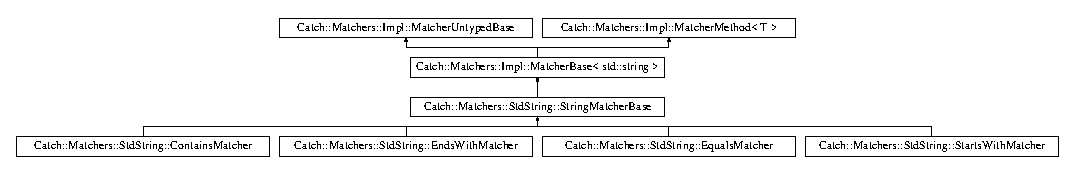
\includegraphics[height=1.879195cm]{struct_catch_1_1_matchers_1_1_std_string_1_1_string_matcher_base}
\end{center}
\end{figure}
\subsection*{Public Member Functions}
\begin{DoxyCompactItemize}
\item 
\mbox{\hyperlink{struct_catch_1_1_matchers_1_1_std_string_1_1_string_matcher_base_a3a9b66bae298ae27058478529b4bb39d}{String\+Matcher\+Base}} (std\+::string const \&operation, \mbox{\hyperlink{struct_catch_1_1_matchers_1_1_std_string_1_1_cased_string}{Cased\+String}} const \&comparator)
\item 
std\+::string \mbox{\hyperlink{struct_catch_1_1_matchers_1_1_std_string_1_1_string_matcher_base_a47af030f8cea42a601ffb1000eea5cca}{describe}} () const override
\end{DoxyCompactItemize}
\subsection*{Public Attributes}
\begin{DoxyCompactItemize}
\item 
\mbox{\hyperlink{struct_catch_1_1_matchers_1_1_std_string_1_1_cased_string}{Cased\+String}} \mbox{\hyperlink{struct_catch_1_1_matchers_1_1_std_string_1_1_string_matcher_base_a17c9f0fe40587070ffe998c193742831}{m\+\_\+comparator}}
\item 
std\+::string \mbox{\hyperlink{struct_catch_1_1_matchers_1_1_std_string_1_1_string_matcher_base_a7a25c4b7d863e9a1c406d81efd0f83ca}{m\+\_\+operation}}
\end{DoxyCompactItemize}
\subsection*{Additional Inherited Members}


\subsection{Constructor \& Destructor Documentation}
\mbox{\Hypertarget{struct_catch_1_1_matchers_1_1_std_string_1_1_string_matcher_base_a3a9b66bae298ae27058478529b4bb39d}\label{struct_catch_1_1_matchers_1_1_std_string_1_1_string_matcher_base_a3a9b66bae298ae27058478529b4bb39d}} 
\index{Catch\+::\+Matchers\+::\+Std\+String\+::\+String\+Matcher\+Base@{Catch\+::\+Matchers\+::\+Std\+String\+::\+String\+Matcher\+Base}!String\+Matcher\+Base@{String\+Matcher\+Base}}
\index{String\+Matcher\+Base@{String\+Matcher\+Base}!Catch\+::\+Matchers\+::\+Std\+String\+::\+String\+Matcher\+Base@{Catch\+::\+Matchers\+::\+Std\+String\+::\+String\+Matcher\+Base}}
\subsubsection{\texorpdfstring{String\+Matcher\+Base()}{StringMatcherBase()}}
{\footnotesize\ttfamily Catch\+::\+Matchers\+::\+Std\+String\+::\+String\+Matcher\+Base\+::\+String\+Matcher\+Base (\begin{DoxyParamCaption}\item[{std\+::string const \&}]{operation,  }\item[{\mbox{\hyperlink{struct_catch_1_1_matchers_1_1_std_string_1_1_cased_string}{Cased\+String}} const \&}]{comparator }\end{DoxyParamCaption})}



\subsection{Member Function Documentation}
\mbox{\Hypertarget{struct_catch_1_1_matchers_1_1_std_string_1_1_string_matcher_base_a47af030f8cea42a601ffb1000eea5cca}\label{struct_catch_1_1_matchers_1_1_std_string_1_1_string_matcher_base_a47af030f8cea42a601ffb1000eea5cca}} 
\index{Catch\+::\+Matchers\+::\+Std\+String\+::\+String\+Matcher\+Base@{Catch\+::\+Matchers\+::\+Std\+String\+::\+String\+Matcher\+Base}!describe@{describe}}
\index{describe@{describe}!Catch\+::\+Matchers\+::\+Std\+String\+::\+String\+Matcher\+Base@{Catch\+::\+Matchers\+::\+Std\+String\+::\+String\+Matcher\+Base}}
\subsubsection{\texorpdfstring{describe()}{describe()}}
{\footnotesize\ttfamily std\+::string Catch\+::\+Matchers\+::\+Std\+String\+::\+String\+Matcher\+Base\+::describe (\begin{DoxyParamCaption}{ }\end{DoxyParamCaption}) const\hspace{0.3cm}{\ttfamily [override]}, {\ttfamily [virtual]}}



Implements \mbox{\hyperlink{class_catch_1_1_matchers_1_1_impl_1_1_matcher_untyped_base_a91d3a907dbfcbb596077df24f6e11fe2}{Catch\+::\+Matchers\+::\+Impl\+::\+Matcher\+Untyped\+Base}}.



\subsection{Member Data Documentation}
\mbox{\Hypertarget{struct_catch_1_1_matchers_1_1_std_string_1_1_string_matcher_base_a17c9f0fe40587070ffe998c193742831}\label{struct_catch_1_1_matchers_1_1_std_string_1_1_string_matcher_base_a17c9f0fe40587070ffe998c193742831}} 
\index{Catch\+::\+Matchers\+::\+Std\+String\+::\+String\+Matcher\+Base@{Catch\+::\+Matchers\+::\+Std\+String\+::\+String\+Matcher\+Base}!m\+\_\+comparator@{m\+\_\+comparator}}
\index{m\+\_\+comparator@{m\+\_\+comparator}!Catch\+::\+Matchers\+::\+Std\+String\+::\+String\+Matcher\+Base@{Catch\+::\+Matchers\+::\+Std\+String\+::\+String\+Matcher\+Base}}
\subsubsection{\texorpdfstring{m\+\_\+comparator}{m\_comparator}}
{\footnotesize\ttfamily \mbox{\hyperlink{struct_catch_1_1_matchers_1_1_std_string_1_1_cased_string}{Cased\+String}} Catch\+::\+Matchers\+::\+Std\+String\+::\+String\+Matcher\+Base\+::m\+\_\+comparator}

\mbox{\Hypertarget{struct_catch_1_1_matchers_1_1_std_string_1_1_string_matcher_base_a7a25c4b7d863e9a1c406d81efd0f83ca}\label{struct_catch_1_1_matchers_1_1_std_string_1_1_string_matcher_base_a7a25c4b7d863e9a1c406d81efd0f83ca}} 
\index{Catch\+::\+Matchers\+::\+Std\+String\+::\+String\+Matcher\+Base@{Catch\+::\+Matchers\+::\+Std\+String\+::\+String\+Matcher\+Base}!m\+\_\+operation@{m\+\_\+operation}}
\index{m\+\_\+operation@{m\+\_\+operation}!Catch\+::\+Matchers\+::\+Std\+String\+::\+String\+Matcher\+Base@{Catch\+::\+Matchers\+::\+Std\+String\+::\+String\+Matcher\+Base}}
\subsubsection{\texorpdfstring{m\+\_\+operation}{m\_operation}}
{\footnotesize\ttfamily std\+::string Catch\+::\+Matchers\+::\+Std\+String\+::\+String\+Matcher\+Base\+::m\+\_\+operation}



The documentation for this struct was generated from the following file\+:\begin{DoxyCompactItemize}
\item 
D\+:/kouluhommat/\+Advanced Object-\/\+Oriented Programming/lopputyö/\+Battleship/\+Battleship/\mbox{\hyperlink{catch_8hpp}{catch.\+hpp}}\end{DoxyCompactItemize}

\hypertarget{class_catch_1_1_string_ref}{}\section{Catch\+:\+:String\+Ref Class Reference}
\label{class_catch_1_1_string_ref}\index{Catch\+::\+String\+Ref@{Catch\+::\+String\+Ref}}


{\ttfamily \#include $<$catch.\+hpp$>$}

\subsection*{Public Types}
\begin{DoxyCompactItemize}
\item 
using \mbox{\hyperlink{class_catch_1_1_string_ref_a06b4db8fc82b197004291cf370b2ba7c}{size\+\_\+type}} = std\+::size\+\_\+t
\end{DoxyCompactItemize}
\subsection*{Public Member Functions}
\begin{DoxyCompactItemize}
\item 
\mbox{\hyperlink{class_catch_1_1_string_ref_a94319c75df6542327c93a312c6a80754}{String\+Ref}} () noexcept
\item 
\mbox{\hyperlink{class_catch_1_1_string_ref_a2f287267c3a988b288bfd910667c1cfc}{String\+Ref}} (\mbox{\hyperlink{class_catch_1_1_string_ref}{String\+Ref}} const \&other) noexcept
\item 
\mbox{\hyperlink{class_catch_1_1_string_ref_a407d5737b94e5a374add5c2794589733}{String\+Ref}} (\mbox{\hyperlink{class_catch_1_1_string_ref}{String\+Ref}} \&\&other) noexcept
\item 
\mbox{\hyperlink{class_catch_1_1_string_ref_aea45f5089c53adac362bff6bd7c40943}{String\+Ref}} (char const $\ast$raw\+Chars) noexcept
\item 
\mbox{\hyperlink{class_catch_1_1_string_ref_a320bf235274ebb90dd6af80485af2797}{String\+Ref}} (char const $\ast$raw\+Chars, \mbox{\hyperlink{class_catch_1_1_string_ref_a06b4db8fc82b197004291cf370b2ba7c}{size\+\_\+type}} \mbox{\hyperlink{class_catch_1_1_string_ref_ae084d72cb2952cee61a63ef36611d0ad}{size}}) noexcept
\item 
\mbox{\hyperlink{class_catch_1_1_string_ref_a7fe41469048f906e9a847798cd335f23}{String\+Ref}} (std\+::string const \&std\+String) noexcept
\item 
\mbox{\hyperlink{class_catch_1_1_string_ref_a387795c6d883d7281befe5e82920faf8}{$\sim$\+String\+Ref}} () noexcept
\item 
auto \mbox{\hyperlink{class_catch_1_1_string_ref_a14d5a1983e33c51c6b5fd33bffbebabb}{operator=}} (\mbox{\hyperlink{class_catch_1_1_string_ref}{String\+Ref}} const \&other) noexcept -\/$>$ \mbox{\hyperlink{class_catch_1_1_string_ref}{String\+Ref}} \&
\item 
\mbox{\hyperlink{class_catch_1_1_string_ref_ad9fde21785affacc32d7da7a70d74e93}{operator std\+::string}} () const
\item 
void \mbox{\hyperlink{class_catch_1_1_string_ref_a8a843e39ad3560d10a80524ed926ed63}{swap}} (\mbox{\hyperlink{class_catch_1_1_string_ref}{String\+Ref}} \&other) noexcept
\item 
auto \mbox{\hyperlink{class_catch_1_1_string_ref_aabb30149ab961187e4b3ff3394bf6e73}{operator==}} (\mbox{\hyperlink{class_catch_1_1_string_ref}{String\+Ref}} const \&other) const noexcept -\/$>$ bool
\item 
auto \mbox{\hyperlink{class_catch_1_1_string_ref_aaa6c8bf61c4628034c19763d1c8ad215}{operator!=}} (\mbox{\hyperlink{class_catch_1_1_string_ref}{String\+Ref}} const \&other) const noexcept -\/$>$ bool
\item 
auto \mbox{\hyperlink{class_catch_1_1_string_ref_a4ba2e01eec1f0f56c257d213c796ab3b}{operator\mbox{[}$\,$\mbox{]}}} (\mbox{\hyperlink{class_catch_1_1_string_ref_a06b4db8fc82b197004291cf370b2ba7c}{size\+\_\+type}} index) const noexcept -\/$>$ char
\item 
auto \mbox{\hyperlink{class_catch_1_1_string_ref_ac6b68b9dc1e1dec69e884e3f7be581bd}{empty}} () const noexcept -\/$>$ bool
\item 
auto \mbox{\hyperlink{class_catch_1_1_string_ref_ae084d72cb2952cee61a63ef36611d0ad}{size}} () const noexcept -\/$>$ \mbox{\hyperlink{class_catch_1_1_string_ref_a06b4db8fc82b197004291cf370b2ba7c}{size\+\_\+type}}
\item 
auto \mbox{\hyperlink{class_catch_1_1_string_ref_a6a6cac7430e626ffdd7550a081e8168f}{number\+Of\+Characters}} () const noexcept -\/$>$ \mbox{\hyperlink{class_catch_1_1_string_ref_a06b4db8fc82b197004291cf370b2ba7c}{size\+\_\+type}}
\item 
auto \mbox{\hyperlink{class_catch_1_1_string_ref_a1669cb2765e820ca258159676cbd82a5}{c\+\_\+str}} () const -\/$>$ char const $\ast$
\item 
auto \mbox{\hyperlink{class_catch_1_1_string_ref_a248568b467cf6599320903ae613c8eee}{substr}} (\mbox{\hyperlink{class_catch_1_1_string_ref_a06b4db8fc82b197004291cf370b2ba7c}{size\+\_\+type}} start, \mbox{\hyperlink{class_catch_1_1_string_ref_a06b4db8fc82b197004291cf370b2ba7c}{size\+\_\+type}} \mbox{\hyperlink{class_catch_1_1_string_ref_ae084d72cb2952cee61a63ef36611d0ad}{size}}) const noexcept -\/$>$ \mbox{\hyperlink{class_catch_1_1_string_ref}{String\+Ref}}
\item 
auto \mbox{\hyperlink{class_catch_1_1_string_ref_aee240387305ca8b249169d79f36e7002}{current\+Data}} () const noexcept -\/$>$ char const $\ast$
\end{DoxyCompactItemize}
\subsection*{Friends}
\begin{DoxyCompactItemize}
\item 
struct \mbox{\hyperlink{class_catch_1_1_string_ref_a420e64e1652de1b0d427775781b018f5}{String\+Ref\+Test\+Access}}
\end{DoxyCompactItemize}


\subsection{Detailed Description}
A non-\/owning string class (similar to the forthcoming std\+::string\+\_\+view) Note that, because a \mbox{\hyperlink{class_catch_1_1_string_ref}{String\+Ref}} may be a substring of another string, it may not be null terminated. \mbox{\hyperlink{class_catch_1_1_string_ref_a1669cb2765e820ca258159676cbd82a5}{c\+\_\+str()}} must return a null terminated string, however, and so the \mbox{\hyperlink{class_catch_1_1_string_ref}{String\+Ref}} will internally take ownership (taking a copy), if necessary. In theory this ownership is not externally visible -\/ but it does mean (substring) String\+Refs should not be shared between threads. 

\subsection{Member Typedef Documentation}
\mbox{\Hypertarget{class_catch_1_1_string_ref_a06b4db8fc82b197004291cf370b2ba7c}\label{class_catch_1_1_string_ref_a06b4db8fc82b197004291cf370b2ba7c}} 
\index{Catch\+::\+String\+Ref@{Catch\+::\+String\+Ref}!size\+\_\+type@{size\+\_\+type}}
\index{size\+\_\+type@{size\+\_\+type}!Catch\+::\+String\+Ref@{Catch\+::\+String\+Ref}}
\subsubsection{\texorpdfstring{size\+\_\+type}{size\_type}}
{\footnotesize\ttfamily using \mbox{\hyperlink{class_catch_1_1_string_ref_a06b4db8fc82b197004291cf370b2ba7c}{Catch\+::\+String\+Ref\+::size\+\_\+type}} =  std\+::size\+\_\+t}



\subsection{Constructor \& Destructor Documentation}
\mbox{\Hypertarget{class_catch_1_1_string_ref_a94319c75df6542327c93a312c6a80754}\label{class_catch_1_1_string_ref_a94319c75df6542327c93a312c6a80754}} 
\index{Catch\+::\+String\+Ref@{Catch\+::\+String\+Ref}!String\+Ref@{String\+Ref}}
\index{String\+Ref@{String\+Ref}!Catch\+::\+String\+Ref@{Catch\+::\+String\+Ref}}
\subsubsection{\texorpdfstring{String\+Ref()}{StringRef()}\hspace{0.1cm}{\footnotesize\ttfamily [1/6]}}
{\footnotesize\ttfamily Catch\+::\+String\+Ref\+::\+String\+Ref (\begin{DoxyParamCaption}{ }\end{DoxyParamCaption})\hspace{0.3cm}{\ttfamily [inline]}, {\ttfamily [noexcept]}}

\mbox{\Hypertarget{class_catch_1_1_string_ref_a2f287267c3a988b288bfd910667c1cfc}\label{class_catch_1_1_string_ref_a2f287267c3a988b288bfd910667c1cfc}} 
\index{Catch\+::\+String\+Ref@{Catch\+::\+String\+Ref}!String\+Ref@{String\+Ref}}
\index{String\+Ref@{String\+Ref}!Catch\+::\+String\+Ref@{Catch\+::\+String\+Ref}}
\subsubsection{\texorpdfstring{String\+Ref()}{StringRef()}\hspace{0.1cm}{\footnotesize\ttfamily [2/6]}}
{\footnotesize\ttfamily Catch\+::\+String\+Ref\+::\+String\+Ref (\begin{DoxyParamCaption}\item[{\mbox{\hyperlink{class_catch_1_1_string_ref}{String\+Ref}} const \&}]{other }\end{DoxyParamCaption})\hspace{0.3cm}{\ttfamily [inline]}, {\ttfamily [noexcept]}}

\mbox{\Hypertarget{class_catch_1_1_string_ref_a407d5737b94e5a374add5c2794589733}\label{class_catch_1_1_string_ref_a407d5737b94e5a374add5c2794589733}} 
\index{Catch\+::\+String\+Ref@{Catch\+::\+String\+Ref}!String\+Ref@{String\+Ref}}
\index{String\+Ref@{String\+Ref}!Catch\+::\+String\+Ref@{Catch\+::\+String\+Ref}}
\subsubsection{\texorpdfstring{String\+Ref()}{StringRef()}\hspace{0.1cm}{\footnotesize\ttfamily [3/6]}}
{\footnotesize\ttfamily Catch\+::\+String\+Ref\+::\+String\+Ref (\begin{DoxyParamCaption}\item[{\mbox{\hyperlink{class_catch_1_1_string_ref}{String\+Ref}} \&\&}]{other }\end{DoxyParamCaption})\hspace{0.3cm}{\ttfamily [inline]}, {\ttfamily [noexcept]}}

\mbox{\Hypertarget{class_catch_1_1_string_ref_aea45f5089c53adac362bff6bd7c40943}\label{class_catch_1_1_string_ref_aea45f5089c53adac362bff6bd7c40943}} 
\index{Catch\+::\+String\+Ref@{Catch\+::\+String\+Ref}!String\+Ref@{String\+Ref}}
\index{String\+Ref@{String\+Ref}!Catch\+::\+String\+Ref@{Catch\+::\+String\+Ref}}
\subsubsection{\texorpdfstring{String\+Ref()}{StringRef()}\hspace{0.1cm}{\footnotesize\ttfamily [4/6]}}
{\footnotesize\ttfamily Catch\+::\+String\+Ref\+::\+String\+Ref (\begin{DoxyParamCaption}\item[{char const $\ast$}]{raw\+Chars }\end{DoxyParamCaption})\hspace{0.3cm}{\ttfamily [noexcept]}}

\mbox{\Hypertarget{class_catch_1_1_string_ref_a320bf235274ebb90dd6af80485af2797}\label{class_catch_1_1_string_ref_a320bf235274ebb90dd6af80485af2797}} 
\index{Catch\+::\+String\+Ref@{Catch\+::\+String\+Ref}!String\+Ref@{String\+Ref}}
\index{String\+Ref@{String\+Ref}!Catch\+::\+String\+Ref@{Catch\+::\+String\+Ref}}
\subsubsection{\texorpdfstring{String\+Ref()}{StringRef()}\hspace{0.1cm}{\footnotesize\ttfamily [5/6]}}
{\footnotesize\ttfamily Catch\+::\+String\+Ref\+::\+String\+Ref (\begin{DoxyParamCaption}\item[{char const $\ast$}]{raw\+Chars,  }\item[{\mbox{\hyperlink{class_catch_1_1_string_ref_a06b4db8fc82b197004291cf370b2ba7c}{size\+\_\+type}}}]{size }\end{DoxyParamCaption})\hspace{0.3cm}{\ttfamily [inline]}, {\ttfamily [noexcept]}}

\mbox{\Hypertarget{class_catch_1_1_string_ref_a7fe41469048f906e9a847798cd335f23}\label{class_catch_1_1_string_ref_a7fe41469048f906e9a847798cd335f23}} 
\index{Catch\+::\+String\+Ref@{Catch\+::\+String\+Ref}!String\+Ref@{String\+Ref}}
\index{String\+Ref@{String\+Ref}!Catch\+::\+String\+Ref@{Catch\+::\+String\+Ref}}
\subsubsection{\texorpdfstring{String\+Ref()}{StringRef()}\hspace{0.1cm}{\footnotesize\ttfamily [6/6]}}
{\footnotesize\ttfamily Catch\+::\+String\+Ref\+::\+String\+Ref (\begin{DoxyParamCaption}\item[{std\+::string const \&}]{std\+String }\end{DoxyParamCaption})\hspace{0.3cm}{\ttfamily [inline]}, {\ttfamily [noexcept]}}

\mbox{\Hypertarget{class_catch_1_1_string_ref_a387795c6d883d7281befe5e82920faf8}\label{class_catch_1_1_string_ref_a387795c6d883d7281befe5e82920faf8}} 
\index{Catch\+::\+String\+Ref@{Catch\+::\+String\+Ref}!````~String\+Ref@{$\sim$\+String\+Ref}}
\index{````~String\+Ref@{$\sim$\+String\+Ref}!Catch\+::\+String\+Ref@{Catch\+::\+String\+Ref}}
\subsubsection{\texorpdfstring{$\sim$\+String\+Ref()}{~StringRef()}}
{\footnotesize\ttfamily Catch\+::\+String\+Ref\+::$\sim$\+String\+Ref (\begin{DoxyParamCaption}{ }\end{DoxyParamCaption})\hspace{0.3cm}{\ttfamily [inline]}, {\ttfamily [noexcept]}}



\subsection{Member Function Documentation}
\mbox{\Hypertarget{class_catch_1_1_string_ref_a1669cb2765e820ca258159676cbd82a5}\label{class_catch_1_1_string_ref_a1669cb2765e820ca258159676cbd82a5}} 
\index{Catch\+::\+String\+Ref@{Catch\+::\+String\+Ref}!c\+\_\+str@{c\+\_\+str}}
\index{c\+\_\+str@{c\+\_\+str}!Catch\+::\+String\+Ref@{Catch\+::\+String\+Ref}}
\subsubsection{\texorpdfstring{c\+\_\+str()}{c\_str()}}
{\footnotesize\ttfamily auto Catch\+::\+String\+Ref\+::c\+\_\+str (\begin{DoxyParamCaption}{ }\end{DoxyParamCaption}) const -\/$>$  char const $\ast$}

\mbox{\Hypertarget{class_catch_1_1_string_ref_aee240387305ca8b249169d79f36e7002}\label{class_catch_1_1_string_ref_aee240387305ca8b249169d79f36e7002}} 
\index{Catch\+::\+String\+Ref@{Catch\+::\+String\+Ref}!current\+Data@{current\+Data}}
\index{current\+Data@{current\+Data}!Catch\+::\+String\+Ref@{Catch\+::\+String\+Ref}}
\subsubsection{\texorpdfstring{current\+Data()}{currentData()}}
{\footnotesize\ttfamily auto Catch\+::\+String\+Ref\+::current\+Data (\begin{DoxyParamCaption}{ }\end{DoxyParamCaption}) const -\/$>$  char const $\ast$\hspace{0.3cm}{\ttfamily [noexcept]}}

\mbox{\Hypertarget{class_catch_1_1_string_ref_ac6b68b9dc1e1dec69e884e3f7be581bd}\label{class_catch_1_1_string_ref_ac6b68b9dc1e1dec69e884e3f7be581bd}} 
\index{Catch\+::\+String\+Ref@{Catch\+::\+String\+Ref}!empty@{empty}}
\index{empty@{empty}!Catch\+::\+String\+Ref@{Catch\+::\+String\+Ref}}
\subsubsection{\texorpdfstring{empty()}{empty()}}
{\footnotesize\ttfamily auto Catch\+::\+String\+Ref\+::empty (\begin{DoxyParamCaption}{ }\end{DoxyParamCaption}) const -\/$>$ bool \hspace{0.3cm}{\ttfamily [inline]}, {\ttfamily [noexcept]}}

\mbox{\Hypertarget{class_catch_1_1_string_ref_a6a6cac7430e626ffdd7550a081e8168f}\label{class_catch_1_1_string_ref_a6a6cac7430e626ffdd7550a081e8168f}} 
\index{Catch\+::\+String\+Ref@{Catch\+::\+String\+Ref}!number\+Of\+Characters@{number\+Of\+Characters}}
\index{number\+Of\+Characters@{number\+Of\+Characters}!Catch\+::\+String\+Ref@{Catch\+::\+String\+Ref}}
\subsubsection{\texorpdfstring{number\+Of\+Characters()}{numberOfCharacters()}}
{\footnotesize\ttfamily auto Catch\+::\+String\+Ref\+::number\+Of\+Characters (\begin{DoxyParamCaption}{ }\end{DoxyParamCaption}) const -\/$>$  \mbox{\hyperlink{class_catch_1_1_string_ref_a06b4db8fc82b197004291cf370b2ba7c}{size\+\_\+type}}\hspace{0.3cm}{\ttfamily [noexcept]}}

\mbox{\Hypertarget{class_catch_1_1_string_ref_ad9fde21785affacc32d7da7a70d74e93}\label{class_catch_1_1_string_ref_ad9fde21785affacc32d7da7a70d74e93}} 
\index{Catch\+::\+String\+Ref@{Catch\+::\+String\+Ref}!operator std\+::string@{operator std\+::string}}
\index{operator std\+::string@{operator std\+::string}!Catch\+::\+String\+Ref@{Catch\+::\+String\+Ref}}
\subsubsection{\texorpdfstring{operator std\+::string()}{operator std::string()}}
{\footnotesize\ttfamily Catch\+::\+String\+Ref\+::operator std\+::string (\begin{DoxyParamCaption}{ }\end{DoxyParamCaption}) const}

\mbox{\Hypertarget{class_catch_1_1_string_ref_aaa6c8bf61c4628034c19763d1c8ad215}\label{class_catch_1_1_string_ref_aaa6c8bf61c4628034c19763d1c8ad215}} 
\index{Catch\+::\+String\+Ref@{Catch\+::\+String\+Ref}!operator"!=@{operator"!=}}
\index{operator"!=@{operator"!=}!Catch\+::\+String\+Ref@{Catch\+::\+String\+Ref}}
\subsubsection{\texorpdfstring{operator"!=()}{operator!=()}}
{\footnotesize\ttfamily auto Catch\+::\+String\+Ref\+::operator!= (\begin{DoxyParamCaption}\item[{\mbox{\hyperlink{class_catch_1_1_string_ref}{String\+Ref}} const \&}]{other }\end{DoxyParamCaption}) const -\/$>$  bool\hspace{0.3cm}{\ttfamily [noexcept]}}

\mbox{\Hypertarget{class_catch_1_1_string_ref_a14d5a1983e33c51c6b5fd33bffbebabb}\label{class_catch_1_1_string_ref_a14d5a1983e33c51c6b5fd33bffbebabb}} 
\index{Catch\+::\+String\+Ref@{Catch\+::\+String\+Ref}!operator=@{operator=}}
\index{operator=@{operator=}!Catch\+::\+String\+Ref@{Catch\+::\+String\+Ref}}
\subsubsection{\texorpdfstring{operator=()}{operator=()}}
{\footnotesize\ttfamily auto Catch\+::\+String\+Ref\+::operator= (\begin{DoxyParamCaption}\item[{\mbox{\hyperlink{class_catch_1_1_string_ref}{String\+Ref}} const \&}]{other }\end{DoxyParamCaption}) -\/$>$ \mbox{\hyperlink{class_catch_1_1_string_ref}{String\+Ref}}\& \hspace{0.3cm}{\ttfamily [inline]}, {\ttfamily [noexcept]}}

\mbox{\Hypertarget{class_catch_1_1_string_ref_aabb30149ab961187e4b3ff3394bf6e73}\label{class_catch_1_1_string_ref_aabb30149ab961187e4b3ff3394bf6e73}} 
\index{Catch\+::\+String\+Ref@{Catch\+::\+String\+Ref}!operator==@{operator==}}
\index{operator==@{operator==}!Catch\+::\+String\+Ref@{Catch\+::\+String\+Ref}}
\subsubsection{\texorpdfstring{operator==()}{operator==()}}
{\footnotesize\ttfamily auto Catch\+::\+String\+Ref\+::operator== (\begin{DoxyParamCaption}\item[{\mbox{\hyperlink{class_catch_1_1_string_ref}{String\+Ref}} const \&}]{other }\end{DoxyParamCaption}) const -\/$>$  bool\hspace{0.3cm}{\ttfamily [noexcept]}}

\mbox{\Hypertarget{class_catch_1_1_string_ref_a4ba2e01eec1f0f56c257d213c796ab3b}\label{class_catch_1_1_string_ref_a4ba2e01eec1f0f56c257d213c796ab3b}} 
\index{Catch\+::\+String\+Ref@{Catch\+::\+String\+Ref}!operator\mbox{[}\mbox{]}@{operator[]}}
\index{operator\mbox{[}\mbox{]}@{operator[]}!Catch\+::\+String\+Ref@{Catch\+::\+String\+Ref}}
\subsubsection{\texorpdfstring{operator[]()}{operator[]()}}
{\footnotesize\ttfamily auto Catch\+::\+String\+Ref\+::operator\mbox{[}$\,$\mbox{]} (\begin{DoxyParamCaption}\item[{\mbox{\hyperlink{class_catch_1_1_string_ref_a06b4db8fc82b197004291cf370b2ba7c}{size\+\_\+type}}}]{index }\end{DoxyParamCaption}) const -\/$>$  char\hspace{0.3cm}{\ttfamily [noexcept]}}

\mbox{\Hypertarget{class_catch_1_1_string_ref_ae084d72cb2952cee61a63ef36611d0ad}\label{class_catch_1_1_string_ref_ae084d72cb2952cee61a63ef36611d0ad}} 
\index{Catch\+::\+String\+Ref@{Catch\+::\+String\+Ref}!size@{size}}
\index{size@{size}!Catch\+::\+String\+Ref@{Catch\+::\+String\+Ref}}
\subsubsection{\texorpdfstring{size()}{size()}}
{\footnotesize\ttfamily auto Catch\+::\+String\+Ref\+::size (\begin{DoxyParamCaption}{ }\end{DoxyParamCaption}) const -\/$>$ \mbox{\hyperlink{class_catch_1_1_string_ref_a06b4db8fc82b197004291cf370b2ba7c}{size\+\_\+type}} \hspace{0.3cm}{\ttfamily [inline]}, {\ttfamily [noexcept]}}

\mbox{\Hypertarget{class_catch_1_1_string_ref_a248568b467cf6599320903ae613c8eee}\label{class_catch_1_1_string_ref_a248568b467cf6599320903ae613c8eee}} 
\index{Catch\+::\+String\+Ref@{Catch\+::\+String\+Ref}!substr@{substr}}
\index{substr@{substr}!Catch\+::\+String\+Ref@{Catch\+::\+String\+Ref}}
\subsubsection{\texorpdfstring{substr()}{substr()}}
{\footnotesize\ttfamily auto Catch\+::\+String\+Ref\+::substr (\begin{DoxyParamCaption}\item[{\mbox{\hyperlink{class_catch_1_1_string_ref_a06b4db8fc82b197004291cf370b2ba7c}{size\+\_\+type}}}]{start,  }\item[{\mbox{\hyperlink{class_catch_1_1_string_ref_a06b4db8fc82b197004291cf370b2ba7c}{size\+\_\+type}}}]{size }\end{DoxyParamCaption}) const -\/$>$  \mbox{\hyperlink{class_catch_1_1_string_ref}{String\+Ref}}\hspace{0.3cm}{\ttfamily [noexcept]}}

\mbox{\Hypertarget{class_catch_1_1_string_ref_a8a843e39ad3560d10a80524ed926ed63}\label{class_catch_1_1_string_ref_a8a843e39ad3560d10a80524ed926ed63}} 
\index{Catch\+::\+String\+Ref@{Catch\+::\+String\+Ref}!swap@{swap}}
\index{swap@{swap}!Catch\+::\+String\+Ref@{Catch\+::\+String\+Ref}}
\subsubsection{\texorpdfstring{swap()}{swap()}}
{\footnotesize\ttfamily void Catch\+::\+String\+Ref\+::swap (\begin{DoxyParamCaption}\item[{\mbox{\hyperlink{class_catch_1_1_string_ref}{String\+Ref}} \&}]{other }\end{DoxyParamCaption})\hspace{0.3cm}{\ttfamily [noexcept]}}



\subsection{Friends And Related Function Documentation}
\mbox{\Hypertarget{class_catch_1_1_string_ref_a420e64e1652de1b0d427775781b018f5}\label{class_catch_1_1_string_ref_a420e64e1652de1b0d427775781b018f5}} 
\index{Catch\+::\+String\+Ref@{Catch\+::\+String\+Ref}!String\+Ref\+Test\+Access@{String\+Ref\+Test\+Access}}
\index{String\+Ref\+Test\+Access@{String\+Ref\+Test\+Access}!Catch\+::\+String\+Ref@{Catch\+::\+String\+Ref}}
\subsubsection{\texorpdfstring{String\+Ref\+Test\+Access}{StringRefTestAccess}}
{\footnotesize\ttfamily friend struct String\+Ref\+Test\+Access\hspace{0.3cm}{\ttfamily [friend]}}



The documentation for this class was generated from the following file\+:\begin{DoxyCompactItemize}
\item 
D\+:/kouluhommat/\+Advanced Object-\/\+Oriented Programming/lopputyö/\+Battleship/\+Battleship/\mbox{\hyperlink{catch_8hpp}{catch.\+hpp}}\end{DoxyCompactItemize}

\hypertarget{class_catch_1_1_test_case}{}\section{Catch\+:\+:Test\+Case Class Reference}
\label{class_catch_1_1_test_case}\index{Catch\+::\+Test\+Case@{Catch\+::\+Test\+Case}}
Inheritance diagram for Catch\+:\+:Test\+Case\+:\begin{figure}[H]
\begin{center}
\leavevmode
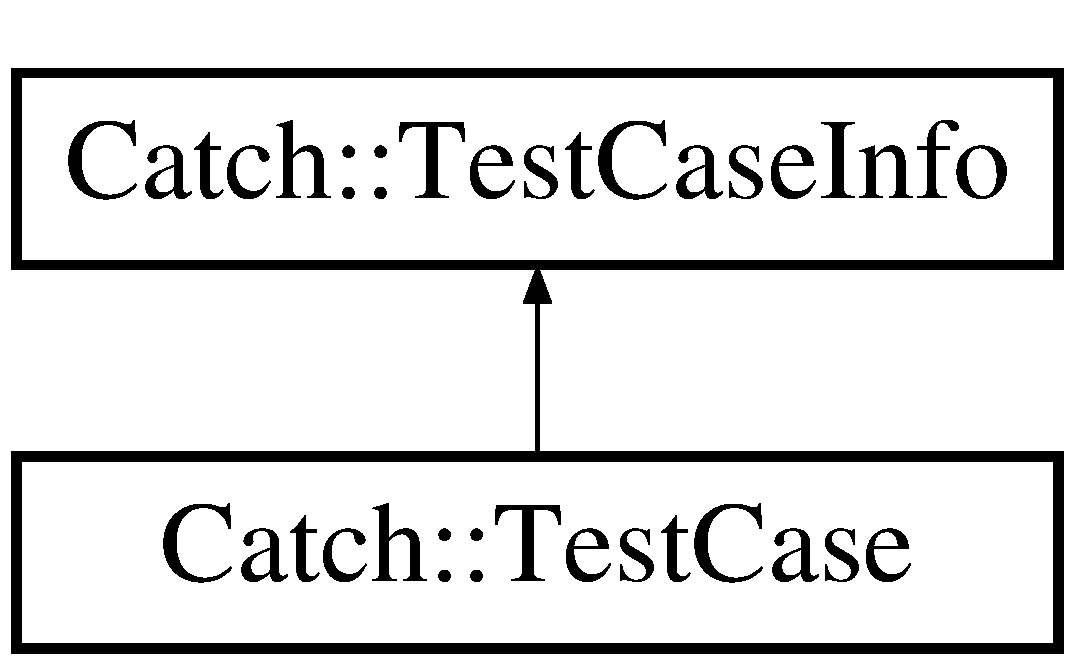
\includegraphics[height=2.000000cm]{class_catch_1_1_test_case}
\end{center}
\end{figure}
\subsection*{Public Member Functions}
\begin{DoxyCompactItemize}
\item 
\mbox{\Hypertarget{class_catch_1_1_test_case_aae5709fc1cb68e19ab0ac27e1ffd6a76}\label{class_catch_1_1_test_case_aae5709fc1cb68e19ab0ac27e1ffd6a76}} 
{\bfseries Test\+Case} (\mbox{\hyperlink{struct_catch_1_1_i_test_invoker}{I\+Test\+Invoker}} $\ast$test\+Case, \mbox{\hyperlink{struct_catch_1_1_test_case_info}{Test\+Case\+Info}} \&\&info)
\item 
\mbox{\Hypertarget{class_catch_1_1_test_case_a0812e8a216d09b087d5874687009f0d6}\label{class_catch_1_1_test_case_a0812e8a216d09b087d5874687009f0d6}} 
\mbox{\hyperlink{class_catch_1_1_test_case}{Test\+Case}} {\bfseries with\+Name} (std\+::string const \&\+\_\+new\+Name) const
\item 
\mbox{\Hypertarget{class_catch_1_1_test_case_a26f346c8446dded0562fe3818ae71651}\label{class_catch_1_1_test_case_a26f346c8446dded0562fe3818ae71651}} 
void {\bfseries invoke} () const
\item 
\mbox{\Hypertarget{class_catch_1_1_test_case_a1ea0d79f49156cebea076fe1ba50d2b6}\label{class_catch_1_1_test_case_a1ea0d79f49156cebea076fe1ba50d2b6}} 
\mbox{\hyperlink{struct_catch_1_1_test_case_info}{Test\+Case\+Info}} const  \& {\bfseries get\+Test\+Case\+Info} () const
\item 
\mbox{\Hypertarget{class_catch_1_1_test_case_a5456d03a90f75292835c158f3a3374a1}\label{class_catch_1_1_test_case_a5456d03a90f75292835c158f3a3374a1}} 
bool {\bfseries operator==} (\mbox{\hyperlink{class_catch_1_1_test_case}{Test\+Case}} const \&other) const
\item 
\mbox{\Hypertarget{class_catch_1_1_test_case_a030e4b9282e9b32e08c8bd5e5cd6fa98}\label{class_catch_1_1_test_case_a030e4b9282e9b32e08c8bd5e5cd6fa98}} 
bool {\bfseries operator$<$} (\mbox{\hyperlink{class_catch_1_1_test_case}{Test\+Case}} const \&other) const
\end{DoxyCompactItemize}
\subsection*{Additional Inherited Members}


The documentation for this class was generated from the following file\+:\begin{DoxyCompactItemize}
\item 
D\+:/kouluhommat/\+Advanced Object-\/\+Oriented Programming/lopputyö/\+Battleship/\+Battleship/catch.\+hpp\end{DoxyCompactItemize}

\hypertarget{struct_catch_1_1_test_case_info}{}\section{Catch\+:\+:Test\+Case\+Info Struct Reference}
\label{struct_catch_1_1_test_case_info}\index{Catch\+::\+Test\+Case\+Info@{Catch\+::\+Test\+Case\+Info}}


{\ttfamily \#include $<$catch.\+hpp$>$}

Inheritance diagram for Catch\+:\+:Test\+Case\+Info\+:\begin{figure}[H]
\begin{center}
\leavevmode
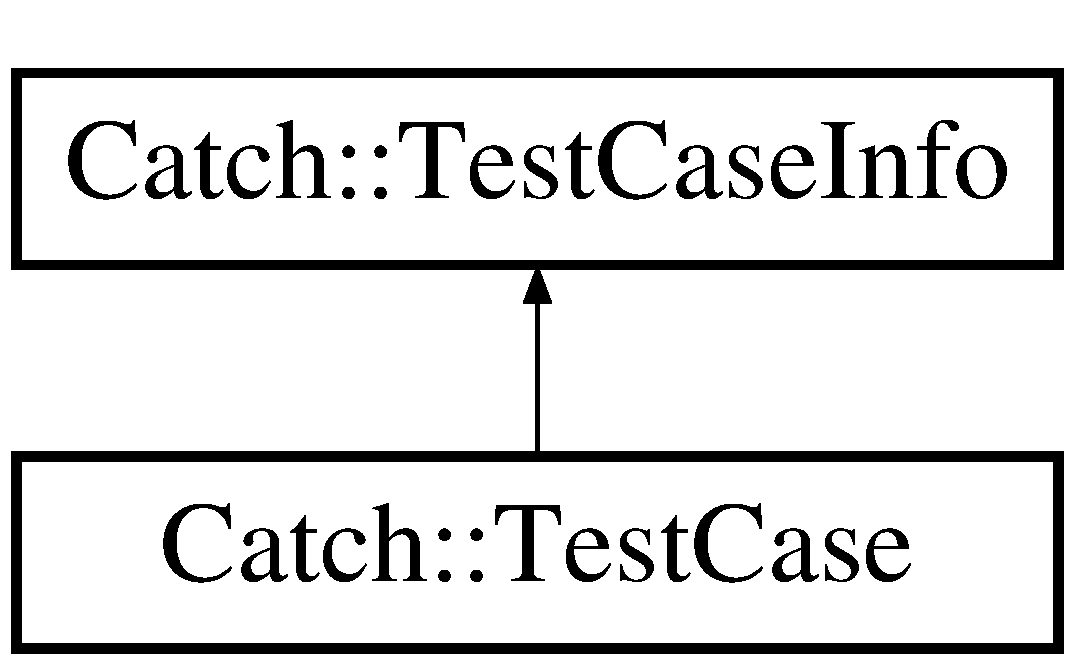
\includegraphics[height=2.000000cm]{struct_catch_1_1_test_case_info}
\end{center}
\end{figure}
\subsection*{Public Types}
\begin{DoxyCompactItemize}
\item 
enum \mbox{\hyperlink{struct_catch_1_1_test_case_info_a39b232f74b4a7a6f2183b96759027eac}{Special\+Properties}} \{ \newline
\mbox{\hyperlink{struct_catch_1_1_test_case_info_a39b232f74b4a7a6f2183b96759027eacaf94e9de5f8ec1e53b1aa761ec564b31a}{None}} = 0, 
\mbox{\hyperlink{struct_catch_1_1_test_case_info_a39b232f74b4a7a6f2183b96759027eacaeda53906c14c3973e0980900c132b8f7}{Is\+Hidden}} = 1 $<$$<$ 1, 
\mbox{\hyperlink{struct_catch_1_1_test_case_info_a39b232f74b4a7a6f2183b96759027eacaf9002285bccfc343935958f3953f4c01}{Should\+Fail}} = 1 $<$$<$ 2, 
\mbox{\hyperlink{struct_catch_1_1_test_case_info_a39b232f74b4a7a6f2183b96759027eacadf1873d3271121cb9f52d7df45b416ca}{May\+Fail}} = 1 $<$$<$ 3, 
\newline
\mbox{\hyperlink{struct_catch_1_1_test_case_info_a39b232f74b4a7a6f2183b96759027eaca4704adf89ed7f7ad653d08f99813a974}{Throws}} = 1 $<$$<$ 4, 
\mbox{\hyperlink{struct_catch_1_1_test_case_info_a39b232f74b4a7a6f2183b96759027eaca06472887b53fda9eb8015d74e7fd2cf1}{Non\+Portable}} = 1 $<$$<$ 5, 
\mbox{\hyperlink{struct_catch_1_1_test_case_info_a39b232f74b4a7a6f2183b96759027eacad0e25e337246ae34d555fe53baf81c16}{Benchmark}} = 1 $<$$<$ 6
 \}
\end{DoxyCompactItemize}
\subsection*{Public Member Functions}
\begin{DoxyCompactItemize}
\item 
\mbox{\hyperlink{struct_catch_1_1_test_case_info_ad1a6b08b5a83d1c5eb4596b727b5305f}{Test\+Case\+Info}} (std\+::string const \&\+\_\+name, std\+::string const \&\+\_\+class\+Name, std\+::string const \&\+\_\+description, std\+::vector$<$ std\+::string $>$ const \&\+\_\+tags, \mbox{\hyperlink{struct_catch_1_1_source_line_info}{Source\+Line\+Info}} const \&\+\_\+line\+Info)
\item 
bool \mbox{\hyperlink{struct_catch_1_1_test_case_info_a934b1a0952700743e99d62ec1731a2e2}{is\+Hidden}} () const
\item 
bool \mbox{\hyperlink{struct_catch_1_1_test_case_info_afc70d4379a2070cc22b693ffe3932c1a}{throws}} () const
\item 
bool \mbox{\hyperlink{struct_catch_1_1_test_case_info_a5f37291295e3a6de2dd85324c941edaf}{ok\+To\+Fail}} () const
\item 
bool \mbox{\hyperlink{struct_catch_1_1_test_case_info_abe33d81233230cdae8afa714688e905b}{expected\+To\+Fail}} () const
\item 
std\+::string \mbox{\hyperlink{struct_catch_1_1_test_case_info_a17506de67fb18e27511c17f8a81119d8}{tags\+As\+String}} () const
\end{DoxyCompactItemize}
\subsection*{Public Attributes}
\begin{DoxyCompactItemize}
\item 
std\+::string \mbox{\hyperlink{struct_catch_1_1_test_case_info_a463794e2f5cfead307c93efd134ade36}{name}}
\item 
std\+::string \mbox{\hyperlink{struct_catch_1_1_test_case_info_a1a5e0825132a38d091defdebbf2f8ce9}{class\+Name}}
\item 
std\+::string \mbox{\hyperlink{struct_catch_1_1_test_case_info_a37fe2db9425bc45f6a33893eac31198e}{description}}
\item 
std\+::vector$<$ std\+::string $>$ \mbox{\hyperlink{struct_catch_1_1_test_case_info_a150a7cbca1dd0c91799ccb14ff822eb0}{tags}}
\item 
std\+::vector$<$ std\+::string $>$ \mbox{\hyperlink{struct_catch_1_1_test_case_info_a844e3de9baf6e53cadfba9733c236bfe}{lcase\+Tags}}
\item 
\mbox{\hyperlink{struct_catch_1_1_source_line_info}{Source\+Line\+Info}} \mbox{\hyperlink{struct_catch_1_1_test_case_info_aa9407b7f442655b51a2aad24b3fa2fd3}{line\+Info}}
\item 
\mbox{\hyperlink{struct_catch_1_1_test_case_info_a39b232f74b4a7a6f2183b96759027eac}{Special\+Properties}} \mbox{\hyperlink{struct_catch_1_1_test_case_info_afc1e84bd7a2e180895a06d9131302af0}{properties}}
\end{DoxyCompactItemize}
\subsection*{Friends}
\begin{DoxyCompactItemize}
\item 
void \mbox{\hyperlink{struct_catch_1_1_test_case_info_a0fe44abaf18ae7c26f98a9fc2b08679c}{set\+Tags}} (\mbox{\hyperlink{struct_catch_1_1_test_case_info}{Test\+Case\+Info}} \&test\+Case\+Info, std\+::vector$<$ std\+::string $>$ \mbox{\hyperlink{struct_catch_1_1_test_case_info_a150a7cbca1dd0c91799ccb14ff822eb0}{tags}})
\end{DoxyCompactItemize}


\subsection{Member Enumeration Documentation}
\mbox{\Hypertarget{struct_catch_1_1_test_case_info_a39b232f74b4a7a6f2183b96759027eac}\label{struct_catch_1_1_test_case_info_a39b232f74b4a7a6f2183b96759027eac}} 
\index{Catch\+::\+Test\+Case\+Info@{Catch\+::\+Test\+Case\+Info}!Special\+Properties@{Special\+Properties}}
\index{Special\+Properties@{Special\+Properties}!Catch\+::\+Test\+Case\+Info@{Catch\+::\+Test\+Case\+Info}}
\subsubsection{\texorpdfstring{Special\+Properties}{SpecialProperties}}
{\footnotesize\ttfamily enum \mbox{\hyperlink{struct_catch_1_1_test_case_info_a39b232f74b4a7a6f2183b96759027eac}{Catch\+::\+Test\+Case\+Info\+::\+Special\+Properties}}}

\begin{DoxyEnumFields}{Enumerator}
\raisebox{\heightof{T}}[0pt][0pt]{\index{None@{None}!Catch\+::\+Test\+Case\+Info@{Catch\+::\+Test\+Case\+Info}}\index{Catch\+::\+Test\+Case\+Info@{Catch\+::\+Test\+Case\+Info}!None@{None}}}\mbox{\Hypertarget{struct_catch_1_1_test_case_info_a39b232f74b4a7a6f2183b96759027eacaf94e9de5f8ec1e53b1aa761ec564b31a}\label{struct_catch_1_1_test_case_info_a39b232f74b4a7a6f2183b96759027eacaf94e9de5f8ec1e53b1aa761ec564b31a}} 
None&\\
\hline

\raisebox{\heightof{T}}[0pt][0pt]{\index{Is\+Hidden@{Is\+Hidden}!Catch\+::\+Test\+Case\+Info@{Catch\+::\+Test\+Case\+Info}}\index{Catch\+::\+Test\+Case\+Info@{Catch\+::\+Test\+Case\+Info}!Is\+Hidden@{Is\+Hidden}}}\mbox{\Hypertarget{struct_catch_1_1_test_case_info_a39b232f74b4a7a6f2183b96759027eacaeda53906c14c3973e0980900c132b8f7}\label{struct_catch_1_1_test_case_info_a39b232f74b4a7a6f2183b96759027eacaeda53906c14c3973e0980900c132b8f7}} 
Is\+Hidden&\\
\hline

\raisebox{\heightof{T}}[0pt][0pt]{\index{Should\+Fail@{Should\+Fail}!Catch\+::\+Test\+Case\+Info@{Catch\+::\+Test\+Case\+Info}}\index{Catch\+::\+Test\+Case\+Info@{Catch\+::\+Test\+Case\+Info}!Should\+Fail@{Should\+Fail}}}\mbox{\Hypertarget{struct_catch_1_1_test_case_info_a39b232f74b4a7a6f2183b96759027eacaf9002285bccfc343935958f3953f4c01}\label{struct_catch_1_1_test_case_info_a39b232f74b4a7a6f2183b96759027eacaf9002285bccfc343935958f3953f4c01}} 
Should\+Fail&\\
\hline

\raisebox{\heightof{T}}[0pt][0pt]{\index{May\+Fail@{May\+Fail}!Catch\+::\+Test\+Case\+Info@{Catch\+::\+Test\+Case\+Info}}\index{Catch\+::\+Test\+Case\+Info@{Catch\+::\+Test\+Case\+Info}!May\+Fail@{May\+Fail}}}\mbox{\Hypertarget{struct_catch_1_1_test_case_info_a39b232f74b4a7a6f2183b96759027eacadf1873d3271121cb9f52d7df45b416ca}\label{struct_catch_1_1_test_case_info_a39b232f74b4a7a6f2183b96759027eacadf1873d3271121cb9f52d7df45b416ca}} 
May\+Fail&\\
\hline

\raisebox{\heightof{T}}[0pt][0pt]{\index{Throws@{Throws}!Catch\+::\+Test\+Case\+Info@{Catch\+::\+Test\+Case\+Info}}\index{Catch\+::\+Test\+Case\+Info@{Catch\+::\+Test\+Case\+Info}!Throws@{Throws}}}\mbox{\Hypertarget{struct_catch_1_1_test_case_info_a39b232f74b4a7a6f2183b96759027eaca4704adf89ed7f7ad653d08f99813a974}\label{struct_catch_1_1_test_case_info_a39b232f74b4a7a6f2183b96759027eaca4704adf89ed7f7ad653d08f99813a974}} 
Throws&\\
\hline

\raisebox{\heightof{T}}[0pt][0pt]{\index{Non\+Portable@{Non\+Portable}!Catch\+::\+Test\+Case\+Info@{Catch\+::\+Test\+Case\+Info}}\index{Catch\+::\+Test\+Case\+Info@{Catch\+::\+Test\+Case\+Info}!Non\+Portable@{Non\+Portable}}}\mbox{\Hypertarget{struct_catch_1_1_test_case_info_a39b232f74b4a7a6f2183b96759027eaca06472887b53fda9eb8015d74e7fd2cf1}\label{struct_catch_1_1_test_case_info_a39b232f74b4a7a6f2183b96759027eaca06472887b53fda9eb8015d74e7fd2cf1}} 
Non\+Portable&\\
\hline

\raisebox{\heightof{T}}[0pt][0pt]{\index{Benchmark@{Benchmark}!Catch\+::\+Test\+Case\+Info@{Catch\+::\+Test\+Case\+Info}}\index{Catch\+::\+Test\+Case\+Info@{Catch\+::\+Test\+Case\+Info}!Benchmark@{Benchmark}}}\mbox{\Hypertarget{struct_catch_1_1_test_case_info_a39b232f74b4a7a6f2183b96759027eacad0e25e337246ae34d555fe53baf81c16}\label{struct_catch_1_1_test_case_info_a39b232f74b4a7a6f2183b96759027eacad0e25e337246ae34d555fe53baf81c16}} 
Benchmark&\\
\hline

\end{DoxyEnumFields}


\subsection{Constructor \& Destructor Documentation}
\mbox{\Hypertarget{struct_catch_1_1_test_case_info_ad1a6b08b5a83d1c5eb4596b727b5305f}\label{struct_catch_1_1_test_case_info_ad1a6b08b5a83d1c5eb4596b727b5305f}} 
\index{Catch\+::\+Test\+Case\+Info@{Catch\+::\+Test\+Case\+Info}!Test\+Case\+Info@{Test\+Case\+Info}}
\index{Test\+Case\+Info@{Test\+Case\+Info}!Catch\+::\+Test\+Case\+Info@{Catch\+::\+Test\+Case\+Info}}
\subsubsection{\texorpdfstring{Test\+Case\+Info()}{TestCaseInfo()}}
{\footnotesize\ttfamily Catch\+::\+Test\+Case\+Info\+::\+Test\+Case\+Info (\begin{DoxyParamCaption}\item[{std\+::string const \&}]{\+\_\+name,  }\item[{std\+::string const \&}]{\+\_\+class\+Name,  }\item[{std\+::string const \&}]{\+\_\+description,  }\item[{std\+::vector$<$ std\+::string $>$ const \&}]{\+\_\+tags,  }\item[{\mbox{\hyperlink{struct_catch_1_1_source_line_info}{Source\+Line\+Info}} const \&}]{\+\_\+line\+Info }\end{DoxyParamCaption})}



\subsection{Member Function Documentation}
\mbox{\Hypertarget{struct_catch_1_1_test_case_info_abe33d81233230cdae8afa714688e905b}\label{struct_catch_1_1_test_case_info_abe33d81233230cdae8afa714688e905b}} 
\index{Catch\+::\+Test\+Case\+Info@{Catch\+::\+Test\+Case\+Info}!expected\+To\+Fail@{expected\+To\+Fail}}
\index{expected\+To\+Fail@{expected\+To\+Fail}!Catch\+::\+Test\+Case\+Info@{Catch\+::\+Test\+Case\+Info}}
\subsubsection{\texorpdfstring{expected\+To\+Fail()}{expectedToFail()}}
{\footnotesize\ttfamily bool Catch\+::\+Test\+Case\+Info\+::expected\+To\+Fail (\begin{DoxyParamCaption}{ }\end{DoxyParamCaption}) const}

\mbox{\Hypertarget{struct_catch_1_1_test_case_info_a934b1a0952700743e99d62ec1731a2e2}\label{struct_catch_1_1_test_case_info_a934b1a0952700743e99d62ec1731a2e2}} 
\index{Catch\+::\+Test\+Case\+Info@{Catch\+::\+Test\+Case\+Info}!is\+Hidden@{is\+Hidden}}
\index{is\+Hidden@{is\+Hidden}!Catch\+::\+Test\+Case\+Info@{Catch\+::\+Test\+Case\+Info}}
\subsubsection{\texorpdfstring{is\+Hidden()}{isHidden()}}
{\footnotesize\ttfamily bool Catch\+::\+Test\+Case\+Info\+::is\+Hidden (\begin{DoxyParamCaption}{ }\end{DoxyParamCaption}) const}

\mbox{\Hypertarget{struct_catch_1_1_test_case_info_a5f37291295e3a6de2dd85324c941edaf}\label{struct_catch_1_1_test_case_info_a5f37291295e3a6de2dd85324c941edaf}} 
\index{Catch\+::\+Test\+Case\+Info@{Catch\+::\+Test\+Case\+Info}!ok\+To\+Fail@{ok\+To\+Fail}}
\index{ok\+To\+Fail@{ok\+To\+Fail}!Catch\+::\+Test\+Case\+Info@{Catch\+::\+Test\+Case\+Info}}
\subsubsection{\texorpdfstring{ok\+To\+Fail()}{okToFail()}}
{\footnotesize\ttfamily bool Catch\+::\+Test\+Case\+Info\+::ok\+To\+Fail (\begin{DoxyParamCaption}{ }\end{DoxyParamCaption}) const}

\mbox{\Hypertarget{struct_catch_1_1_test_case_info_a17506de67fb18e27511c17f8a81119d8}\label{struct_catch_1_1_test_case_info_a17506de67fb18e27511c17f8a81119d8}} 
\index{Catch\+::\+Test\+Case\+Info@{Catch\+::\+Test\+Case\+Info}!tags\+As\+String@{tags\+As\+String}}
\index{tags\+As\+String@{tags\+As\+String}!Catch\+::\+Test\+Case\+Info@{Catch\+::\+Test\+Case\+Info}}
\subsubsection{\texorpdfstring{tags\+As\+String()}{tagsAsString()}}
{\footnotesize\ttfamily std\+::string Catch\+::\+Test\+Case\+Info\+::tags\+As\+String (\begin{DoxyParamCaption}{ }\end{DoxyParamCaption}) const}

\mbox{\Hypertarget{struct_catch_1_1_test_case_info_afc70d4379a2070cc22b693ffe3932c1a}\label{struct_catch_1_1_test_case_info_afc70d4379a2070cc22b693ffe3932c1a}} 
\index{Catch\+::\+Test\+Case\+Info@{Catch\+::\+Test\+Case\+Info}!throws@{throws}}
\index{throws@{throws}!Catch\+::\+Test\+Case\+Info@{Catch\+::\+Test\+Case\+Info}}
\subsubsection{\texorpdfstring{throws()}{throws()}}
{\footnotesize\ttfamily bool Catch\+::\+Test\+Case\+Info\+::throws (\begin{DoxyParamCaption}{ }\end{DoxyParamCaption}) const}



\subsection{Friends And Related Function Documentation}
\mbox{\Hypertarget{struct_catch_1_1_test_case_info_a0fe44abaf18ae7c26f98a9fc2b08679c}\label{struct_catch_1_1_test_case_info_a0fe44abaf18ae7c26f98a9fc2b08679c}} 
\index{Catch\+::\+Test\+Case\+Info@{Catch\+::\+Test\+Case\+Info}!set\+Tags@{set\+Tags}}
\index{set\+Tags@{set\+Tags}!Catch\+::\+Test\+Case\+Info@{Catch\+::\+Test\+Case\+Info}}
\subsubsection{\texorpdfstring{set\+Tags}{setTags}}
{\footnotesize\ttfamily void set\+Tags (\begin{DoxyParamCaption}\item[{\mbox{\hyperlink{struct_catch_1_1_test_case_info}{Test\+Case\+Info}} \&}]{test\+Case\+Info,  }\item[{std\+::vector$<$ std\+::string $>$}]{tags }\end{DoxyParamCaption})\hspace{0.3cm}{\ttfamily [friend]}}



\subsection{Member Data Documentation}
\mbox{\Hypertarget{struct_catch_1_1_test_case_info_a1a5e0825132a38d091defdebbf2f8ce9}\label{struct_catch_1_1_test_case_info_a1a5e0825132a38d091defdebbf2f8ce9}} 
\index{Catch\+::\+Test\+Case\+Info@{Catch\+::\+Test\+Case\+Info}!class\+Name@{class\+Name}}
\index{class\+Name@{class\+Name}!Catch\+::\+Test\+Case\+Info@{Catch\+::\+Test\+Case\+Info}}
\subsubsection{\texorpdfstring{class\+Name}{className}}
{\footnotesize\ttfamily std\+::string Catch\+::\+Test\+Case\+Info\+::class\+Name}

\mbox{\Hypertarget{struct_catch_1_1_test_case_info_a37fe2db9425bc45f6a33893eac31198e}\label{struct_catch_1_1_test_case_info_a37fe2db9425bc45f6a33893eac31198e}} 
\index{Catch\+::\+Test\+Case\+Info@{Catch\+::\+Test\+Case\+Info}!description@{description}}
\index{description@{description}!Catch\+::\+Test\+Case\+Info@{Catch\+::\+Test\+Case\+Info}}
\subsubsection{\texorpdfstring{description}{description}}
{\footnotesize\ttfamily std\+::string Catch\+::\+Test\+Case\+Info\+::description}

\mbox{\Hypertarget{struct_catch_1_1_test_case_info_a844e3de9baf6e53cadfba9733c236bfe}\label{struct_catch_1_1_test_case_info_a844e3de9baf6e53cadfba9733c236bfe}} 
\index{Catch\+::\+Test\+Case\+Info@{Catch\+::\+Test\+Case\+Info}!lcase\+Tags@{lcase\+Tags}}
\index{lcase\+Tags@{lcase\+Tags}!Catch\+::\+Test\+Case\+Info@{Catch\+::\+Test\+Case\+Info}}
\subsubsection{\texorpdfstring{lcase\+Tags}{lcaseTags}}
{\footnotesize\ttfamily std\+::vector$<$std\+::string$>$ Catch\+::\+Test\+Case\+Info\+::lcase\+Tags}

\mbox{\Hypertarget{struct_catch_1_1_test_case_info_aa9407b7f442655b51a2aad24b3fa2fd3}\label{struct_catch_1_1_test_case_info_aa9407b7f442655b51a2aad24b3fa2fd3}} 
\index{Catch\+::\+Test\+Case\+Info@{Catch\+::\+Test\+Case\+Info}!line\+Info@{line\+Info}}
\index{line\+Info@{line\+Info}!Catch\+::\+Test\+Case\+Info@{Catch\+::\+Test\+Case\+Info}}
\subsubsection{\texorpdfstring{line\+Info}{lineInfo}}
{\footnotesize\ttfamily \mbox{\hyperlink{struct_catch_1_1_source_line_info}{Source\+Line\+Info}} Catch\+::\+Test\+Case\+Info\+::line\+Info}

\mbox{\Hypertarget{struct_catch_1_1_test_case_info_a463794e2f5cfead307c93efd134ade36}\label{struct_catch_1_1_test_case_info_a463794e2f5cfead307c93efd134ade36}} 
\index{Catch\+::\+Test\+Case\+Info@{Catch\+::\+Test\+Case\+Info}!name@{name}}
\index{name@{name}!Catch\+::\+Test\+Case\+Info@{Catch\+::\+Test\+Case\+Info}}
\subsubsection{\texorpdfstring{name}{name}}
{\footnotesize\ttfamily std\+::string Catch\+::\+Test\+Case\+Info\+::name}

\mbox{\Hypertarget{struct_catch_1_1_test_case_info_afc1e84bd7a2e180895a06d9131302af0}\label{struct_catch_1_1_test_case_info_afc1e84bd7a2e180895a06d9131302af0}} 
\index{Catch\+::\+Test\+Case\+Info@{Catch\+::\+Test\+Case\+Info}!properties@{properties}}
\index{properties@{properties}!Catch\+::\+Test\+Case\+Info@{Catch\+::\+Test\+Case\+Info}}
\subsubsection{\texorpdfstring{properties}{properties}}
{\footnotesize\ttfamily \mbox{\hyperlink{struct_catch_1_1_test_case_info_a39b232f74b4a7a6f2183b96759027eac}{Special\+Properties}} Catch\+::\+Test\+Case\+Info\+::properties}

\mbox{\Hypertarget{struct_catch_1_1_test_case_info_a150a7cbca1dd0c91799ccb14ff822eb0}\label{struct_catch_1_1_test_case_info_a150a7cbca1dd0c91799ccb14ff822eb0}} 
\index{Catch\+::\+Test\+Case\+Info@{Catch\+::\+Test\+Case\+Info}!tags@{tags}}
\index{tags@{tags}!Catch\+::\+Test\+Case\+Info@{Catch\+::\+Test\+Case\+Info}}
\subsubsection{\texorpdfstring{tags}{tags}}
{\footnotesize\ttfamily std\+::vector$<$std\+::string$>$ Catch\+::\+Test\+Case\+Info\+::tags}



The documentation for this struct was generated from the following file\+:\begin{DoxyCompactItemize}
\item 
D\+:/kouluhommat/\+Advanced Object-\/\+Oriented Programming/lopputyö/\+Battleship/\+Battleship/\mbox{\hyperlink{catch_8hpp}{catch.\+hpp}}\end{DoxyCompactItemize}

\hypertarget{struct_catch_1_1_test_failure_exception}{}\section{Catch\+:\+:Test\+Failure\+Exception Struct Reference}
\label{struct_catch_1_1_test_failure_exception}\index{Catch\+::\+Test\+Failure\+Exception@{Catch\+::\+Test\+Failure\+Exception}}


The documentation for this struct was generated from the following file\+:\begin{DoxyCompactItemize}
\item 
D\+:/kouluhommat/\+Advanced Object-\/\+Oriented Programming/lopputyö/\+Battleship/\+Battleship/catch.\+hpp\end{DoxyCompactItemize}

\hypertarget{class_catch_1_1_test_invoker_as_method}{}\section{Catch\+:\+:Test\+Invoker\+As\+Method$<$ C $>$ Class Template Reference}
\label{class_catch_1_1_test_invoker_as_method}\index{Catch\+::\+Test\+Invoker\+As\+Method$<$ C $>$@{Catch\+::\+Test\+Invoker\+As\+Method$<$ C $>$}}


{\ttfamily \#include $<$catch.\+hpp$>$}

Inheritance diagram for Catch\+:\+:Test\+Invoker\+As\+Method$<$ C $>$\+:\begin{figure}[H]
\begin{center}
\leavevmode
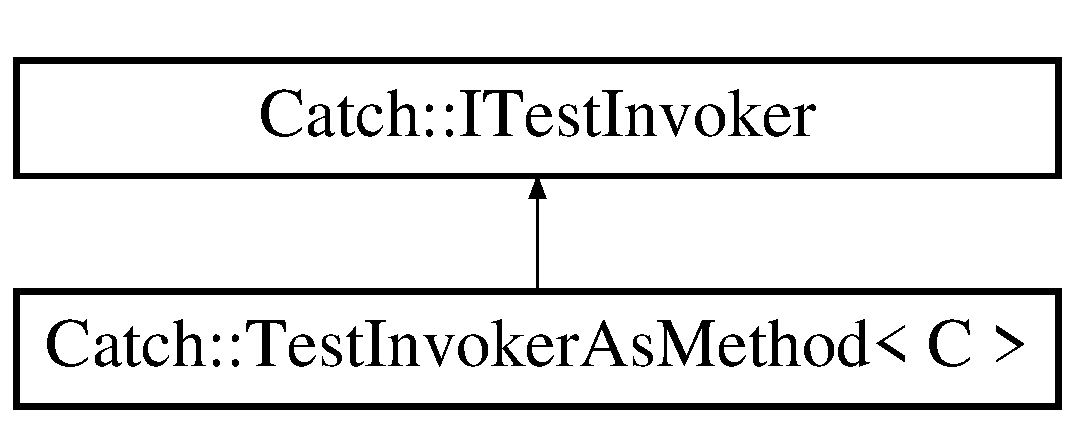
\includegraphics[height=2.000000cm]{class_catch_1_1_test_invoker_as_method}
\end{center}
\end{figure}
\subsection*{Public Member Functions}
\begin{DoxyCompactItemize}
\item 
\mbox{\hyperlink{class_catch_1_1_test_invoker_as_method_a119c4bdbbdd95c42859c18541987a1a4}{Test\+Invoker\+As\+Method}} (void(C\+::$\ast$test\+As\+Method)()) noexcept
\item 
void \mbox{\hyperlink{class_catch_1_1_test_invoker_as_method_a8115a06efe273f4112ec0b5452c1b5f2}{invoke}} () const override
\end{DoxyCompactItemize}


\subsection{Constructor \& Destructor Documentation}
\mbox{\Hypertarget{class_catch_1_1_test_invoker_as_method_a119c4bdbbdd95c42859c18541987a1a4}\label{class_catch_1_1_test_invoker_as_method_a119c4bdbbdd95c42859c18541987a1a4}} 
\index{Catch\+::\+Test\+Invoker\+As\+Method@{Catch\+::\+Test\+Invoker\+As\+Method}!Test\+Invoker\+As\+Method@{Test\+Invoker\+As\+Method}}
\index{Test\+Invoker\+As\+Method@{Test\+Invoker\+As\+Method}!Catch\+::\+Test\+Invoker\+As\+Method@{Catch\+::\+Test\+Invoker\+As\+Method}}
\subsubsection{\texorpdfstring{Test\+Invoker\+As\+Method()}{TestInvokerAsMethod()}}
{\footnotesize\ttfamily template$<$typename C $>$ \\
\mbox{\hyperlink{class_catch_1_1_test_invoker_as_method}{Catch\+::\+Test\+Invoker\+As\+Method}}$<$ C $>$\+::\mbox{\hyperlink{class_catch_1_1_test_invoker_as_method}{Test\+Invoker\+As\+Method}} (\begin{DoxyParamCaption}\item[{void(C\+::$\ast$)()}]{test\+As\+Method }\end{DoxyParamCaption})\hspace{0.3cm}{\ttfamily [inline]}, {\ttfamily [noexcept]}}



\subsection{Member Function Documentation}
\mbox{\Hypertarget{class_catch_1_1_test_invoker_as_method_a8115a06efe273f4112ec0b5452c1b5f2}\label{class_catch_1_1_test_invoker_as_method_a8115a06efe273f4112ec0b5452c1b5f2}} 
\index{Catch\+::\+Test\+Invoker\+As\+Method@{Catch\+::\+Test\+Invoker\+As\+Method}!invoke@{invoke}}
\index{invoke@{invoke}!Catch\+::\+Test\+Invoker\+As\+Method@{Catch\+::\+Test\+Invoker\+As\+Method}}
\subsubsection{\texorpdfstring{invoke()}{invoke()}}
{\footnotesize\ttfamily template$<$typename C $>$ \\
void \mbox{\hyperlink{class_catch_1_1_test_invoker_as_method}{Catch\+::\+Test\+Invoker\+As\+Method}}$<$ C $>$\+::invoke (\begin{DoxyParamCaption}{ }\end{DoxyParamCaption}) const\hspace{0.3cm}{\ttfamily [inline]}, {\ttfamily [override]}, {\ttfamily [virtual]}}



Implements \mbox{\hyperlink{struct_catch_1_1_i_test_invoker_a6fcd5c5b67d6d5ade6491ff33411ca7f}{Catch\+::\+I\+Test\+Invoker}}.



The documentation for this class was generated from the following file\+:\begin{DoxyCompactItemize}
\item 
D\+:/kouluhommat/\+Advanced Object-\/\+Oriented Programming/lopputyö/\+Battleship/\+Battleship/\mbox{\hyperlink{catch_8hpp}{catch.\+hpp}}\end{DoxyCompactItemize}

\hypertarget{class_catch_1_1_timer}{}\section{Catch\+:\+:Timer Class Reference}
\label{class_catch_1_1_timer}\index{Catch\+::\+Timer@{Catch\+::\+Timer}}


{\ttfamily \#include $<$catch.\+hpp$>$}

\subsection*{Public Member Functions}
\begin{DoxyCompactItemize}
\item 
void \mbox{\hyperlink{class_catch_1_1_timer_a0a56e879e43f36c102bf9ea8b5fc8b72}{start}} ()
\item 
auto \mbox{\hyperlink{class_catch_1_1_timer_a57be5d17ca868a2d6fb1eea84de665cf}{get\+Elapsed\+Nanoseconds}} () const -\/$>$ uint64\+\_\+t
\item 
auto \mbox{\hyperlink{class_catch_1_1_timer_a545de17a61a6fee1dbe3de5b0723e5fa}{get\+Elapsed\+Microseconds}} () const -\/$>$ uint64\+\_\+t
\item 
auto \mbox{\hyperlink{class_catch_1_1_timer_a30aaf458dbb59dd8ac8971c9c62e0eac}{get\+Elapsed\+Milliseconds}} () const -\/$>$ unsigned int
\item 
auto \mbox{\hyperlink{class_catch_1_1_timer_a065e37e3c9eb16bd4dcf41971d8deedc}{get\+Elapsed\+Seconds}} () const -\/$>$ double
\end{DoxyCompactItemize}


\subsection{Member Function Documentation}
\mbox{\Hypertarget{class_catch_1_1_timer_a545de17a61a6fee1dbe3de5b0723e5fa}\label{class_catch_1_1_timer_a545de17a61a6fee1dbe3de5b0723e5fa}} 
\index{Catch\+::\+Timer@{Catch\+::\+Timer}!get\+Elapsed\+Microseconds@{get\+Elapsed\+Microseconds}}
\index{get\+Elapsed\+Microseconds@{get\+Elapsed\+Microseconds}!Catch\+::\+Timer@{Catch\+::\+Timer}}
\subsubsection{\texorpdfstring{get\+Elapsed\+Microseconds()}{getElapsedMicroseconds()}}
{\footnotesize\ttfamily auto Catch\+::\+Timer\+::get\+Elapsed\+Microseconds (\begin{DoxyParamCaption}{ }\end{DoxyParamCaption}) const -\/$>$  uint64\+\_\+t}

\mbox{\Hypertarget{class_catch_1_1_timer_a30aaf458dbb59dd8ac8971c9c62e0eac}\label{class_catch_1_1_timer_a30aaf458dbb59dd8ac8971c9c62e0eac}} 
\index{Catch\+::\+Timer@{Catch\+::\+Timer}!get\+Elapsed\+Milliseconds@{get\+Elapsed\+Milliseconds}}
\index{get\+Elapsed\+Milliseconds@{get\+Elapsed\+Milliseconds}!Catch\+::\+Timer@{Catch\+::\+Timer}}
\subsubsection{\texorpdfstring{get\+Elapsed\+Milliseconds()}{getElapsedMilliseconds()}}
{\footnotesize\ttfamily auto Catch\+::\+Timer\+::get\+Elapsed\+Milliseconds (\begin{DoxyParamCaption}{ }\end{DoxyParamCaption}) const -\/$>$  unsigned int}

\mbox{\Hypertarget{class_catch_1_1_timer_a57be5d17ca868a2d6fb1eea84de665cf}\label{class_catch_1_1_timer_a57be5d17ca868a2d6fb1eea84de665cf}} 
\index{Catch\+::\+Timer@{Catch\+::\+Timer}!get\+Elapsed\+Nanoseconds@{get\+Elapsed\+Nanoseconds}}
\index{get\+Elapsed\+Nanoseconds@{get\+Elapsed\+Nanoseconds}!Catch\+::\+Timer@{Catch\+::\+Timer}}
\subsubsection{\texorpdfstring{get\+Elapsed\+Nanoseconds()}{getElapsedNanoseconds()}}
{\footnotesize\ttfamily auto Catch\+::\+Timer\+::get\+Elapsed\+Nanoseconds (\begin{DoxyParamCaption}{ }\end{DoxyParamCaption}) const -\/$>$  uint64\+\_\+t}

\mbox{\Hypertarget{class_catch_1_1_timer_a065e37e3c9eb16bd4dcf41971d8deedc}\label{class_catch_1_1_timer_a065e37e3c9eb16bd4dcf41971d8deedc}} 
\index{Catch\+::\+Timer@{Catch\+::\+Timer}!get\+Elapsed\+Seconds@{get\+Elapsed\+Seconds}}
\index{get\+Elapsed\+Seconds@{get\+Elapsed\+Seconds}!Catch\+::\+Timer@{Catch\+::\+Timer}}
\subsubsection{\texorpdfstring{get\+Elapsed\+Seconds()}{getElapsedSeconds()}}
{\footnotesize\ttfamily auto Catch\+::\+Timer\+::get\+Elapsed\+Seconds (\begin{DoxyParamCaption}{ }\end{DoxyParamCaption}) const -\/$>$  double}

\mbox{\Hypertarget{class_catch_1_1_timer_a0a56e879e43f36c102bf9ea8b5fc8b72}\label{class_catch_1_1_timer_a0a56e879e43f36c102bf9ea8b5fc8b72}} 
\index{Catch\+::\+Timer@{Catch\+::\+Timer}!start@{start}}
\index{start@{start}!Catch\+::\+Timer@{Catch\+::\+Timer}}
\subsubsection{\texorpdfstring{start()}{start()}}
{\footnotesize\ttfamily void Catch\+::\+Timer\+::start (\begin{DoxyParamCaption}{ }\end{DoxyParamCaption})}



The documentation for this class was generated from the following file\+:\begin{DoxyCompactItemize}
\item 
D\+:/kouluhommat/\+Advanced Object-\/\+Oriented Programming/lopputyö/\+Battleship/\+Battleship/\mbox{\hyperlink{catch_8hpp}{catch.\+hpp}}\end{DoxyCompactItemize}

\hypertarget{struct_catch_1_1_totals}{}\section{Catch\+:\+:Totals Struct Reference}
\label{struct_catch_1_1_totals}\index{Catch\+::\+Totals@{Catch\+::\+Totals}}
\subsection*{Public Member Functions}
\begin{DoxyCompactItemize}
\item 
\mbox{\Hypertarget{struct_catch_1_1_totals_a9279ed39139cb7e7b291918a6d08290e}\label{struct_catch_1_1_totals_a9279ed39139cb7e7b291918a6d08290e}} 
\mbox{\hyperlink{struct_catch_1_1_totals}{Totals}} {\bfseries operator-\/} (\mbox{\hyperlink{struct_catch_1_1_totals}{Totals}} const \&other) const
\item 
\mbox{\Hypertarget{struct_catch_1_1_totals_a574015076e54cc405c70b053e3356e43}\label{struct_catch_1_1_totals_a574015076e54cc405c70b053e3356e43}} 
\mbox{\hyperlink{struct_catch_1_1_totals}{Totals}} \& {\bfseries operator+=} (\mbox{\hyperlink{struct_catch_1_1_totals}{Totals}} const \&other)
\item 
\mbox{\Hypertarget{struct_catch_1_1_totals_a1a94a654f5f3786b75695e081fc9bca2}\label{struct_catch_1_1_totals_a1a94a654f5f3786b75695e081fc9bca2}} 
\mbox{\hyperlink{struct_catch_1_1_totals}{Totals}} {\bfseries delta} (\mbox{\hyperlink{struct_catch_1_1_totals}{Totals}} const \&prev\+Totals) const
\end{DoxyCompactItemize}
\subsection*{Public Attributes}
\begin{DoxyCompactItemize}
\item 
\mbox{\Hypertarget{struct_catch_1_1_totals_a6ea14c7de7ea735a14f172a26e08a239}\label{struct_catch_1_1_totals_a6ea14c7de7ea735a14f172a26e08a239}} 
int {\bfseries error} = 0
\item 
\mbox{\Hypertarget{struct_catch_1_1_totals_a885ded66df752147b30c3d45aa602ec9}\label{struct_catch_1_1_totals_a885ded66df752147b30c3d45aa602ec9}} 
\mbox{\hyperlink{struct_catch_1_1_counts}{Counts}} {\bfseries assertions}
\item 
\mbox{\Hypertarget{struct_catch_1_1_totals_adb195fe477aedee2ecea88c888f16506}\label{struct_catch_1_1_totals_adb195fe477aedee2ecea88c888f16506}} 
\mbox{\hyperlink{struct_catch_1_1_counts}{Counts}} {\bfseries test\+Cases}
\end{DoxyCompactItemize}


The documentation for this struct was generated from the following file\+:\begin{DoxyCompactItemize}
\item 
D\+:/kouluhommat/\+Advanced Object-\/\+Oriented Programming/lopputyö/\+Battleship/\+Battleship/catch.\+hpp\end{DoxyCompactItemize}

\hypertarget{class_catch_1_1_unary_expr}{}\section{Catch\+:\+:Unary\+Expr$<$ LhsT $>$ Class Template Reference}
\label{class_catch_1_1_unary_expr}\index{Catch\+::\+Unary\+Expr$<$ Lhs\+T $>$@{Catch\+::\+Unary\+Expr$<$ Lhs\+T $>$}}


{\ttfamily \#include $<$catch.\+hpp$>$}

Inheritance diagram for Catch\+:\+:Unary\+Expr$<$ LhsT $>$\+:\begin{figure}[H]
\begin{center}
\leavevmode
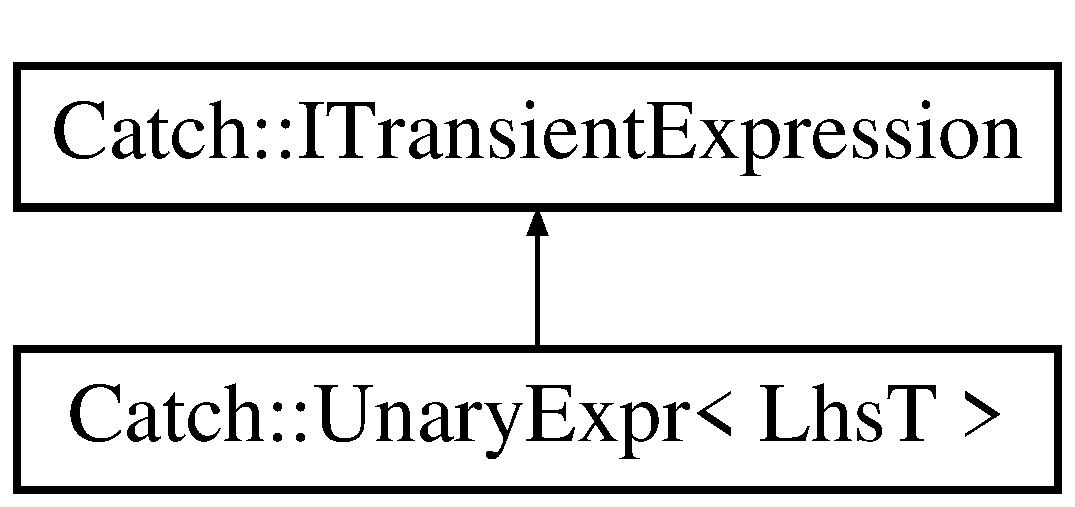
\includegraphics[height=2.000000cm]{class_catch_1_1_unary_expr}
\end{center}
\end{figure}
\subsection*{Public Member Functions}
\begin{DoxyCompactItemize}
\item 
\mbox{\hyperlink{class_catch_1_1_unary_expr_ae02f666a1e64da728628aa2033e1d6e7}{Unary\+Expr}} (LhsT lhs)
\end{DoxyCompactItemize}
\subsection*{Additional Inherited Members}


\subsection{Constructor \& Destructor Documentation}
\mbox{\Hypertarget{class_catch_1_1_unary_expr_ae02f666a1e64da728628aa2033e1d6e7}\label{class_catch_1_1_unary_expr_ae02f666a1e64da728628aa2033e1d6e7}} 
\index{Catch\+::\+Unary\+Expr@{Catch\+::\+Unary\+Expr}!Unary\+Expr@{Unary\+Expr}}
\index{Unary\+Expr@{Unary\+Expr}!Catch\+::\+Unary\+Expr@{Catch\+::\+Unary\+Expr}}
\subsubsection{\texorpdfstring{Unary\+Expr()}{UnaryExpr()}}
{\footnotesize\ttfamily template$<$typename LhsT $>$ \\
\mbox{\hyperlink{class_catch_1_1_unary_expr}{Catch\+::\+Unary\+Expr}}$<$ LhsT $>$\+::\mbox{\hyperlink{class_catch_1_1_unary_expr}{Unary\+Expr}} (\begin{DoxyParamCaption}\item[{LhsT}]{lhs }\end{DoxyParamCaption})\hspace{0.3cm}{\ttfamily [inline]}, {\ttfamily [explicit]}}



The documentation for this class was generated from the following file\+:\begin{DoxyCompactItemize}
\item 
D\+:/kouluhommat/\+Advanced Object-\/\+Oriented Programming/lopputyö/\+Battleship/\+Battleship/\mbox{\hyperlink{catch_8hpp}{catch.\+hpp}}\end{DoxyCompactItemize}

\hypertarget{struct_catch_1_1_matchers_1_1_vector_1_1_unordered_equals_matcher}{}\section{Catch\+:\+:Matchers\+:\+:Vector\+:\+:Unordered\+Equals\+Matcher$<$ T $>$ Struct Template Reference}
\label{struct_catch_1_1_matchers_1_1_vector_1_1_unordered_equals_matcher}\index{Catch\+::\+Matchers\+::\+Vector\+::\+Unordered\+Equals\+Matcher$<$ T $>$@{Catch\+::\+Matchers\+::\+Vector\+::\+Unordered\+Equals\+Matcher$<$ T $>$}}
Inheritance diagram for Catch\+:\+:Matchers\+:\+:Vector\+:\+:Unordered\+Equals\+Matcher$<$ T $>$\+:\begin{figure}[H]
\begin{center}
\leavevmode
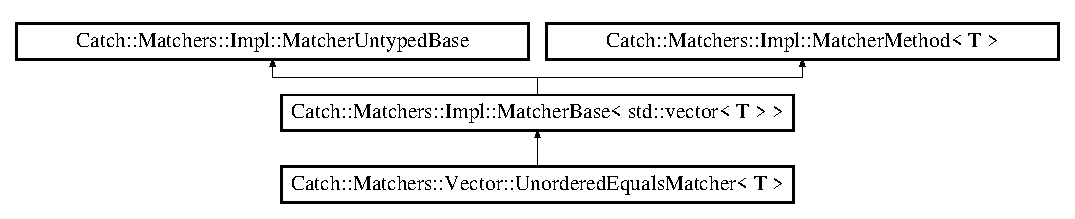
\includegraphics[height=2.492581cm]{struct_catch_1_1_matchers_1_1_vector_1_1_unordered_equals_matcher}
\end{center}
\end{figure}
\subsection*{Public Member Functions}
\begin{DoxyCompactItemize}
\item 
\mbox{\Hypertarget{struct_catch_1_1_matchers_1_1_vector_1_1_unordered_equals_matcher_a525905639b2b15b52ddb0bf14bfa19da}\label{struct_catch_1_1_matchers_1_1_vector_1_1_unordered_equals_matcher_a525905639b2b15b52ddb0bf14bfa19da}} 
{\bfseries Unordered\+Equals\+Matcher} (std\+::vector$<$ T $>$ const \&target)
\item 
\mbox{\Hypertarget{struct_catch_1_1_matchers_1_1_vector_1_1_unordered_equals_matcher_a3ccdd9dd2cd8bdbb8bb121acbb9cb358}\label{struct_catch_1_1_matchers_1_1_vector_1_1_unordered_equals_matcher_a3ccdd9dd2cd8bdbb8bb121acbb9cb358}} 
bool {\bfseries match} (std\+::vector$<$ T $>$ const \&vec) const override
\item 
\mbox{\Hypertarget{struct_catch_1_1_matchers_1_1_vector_1_1_unordered_equals_matcher_a7202d811200317abc58c844f663823df}\label{struct_catch_1_1_matchers_1_1_vector_1_1_unordered_equals_matcher_a7202d811200317abc58c844f663823df}} 
std\+::string {\bfseries describe} () const override
\end{DoxyCompactItemize}
\subsection*{Additional Inherited Members}


The documentation for this struct was generated from the following file\+:\begin{DoxyCompactItemize}
\item 
D\+:/kouluhommat/\+Advanced Object-\/\+Oriented Programming/lopputyö/\+Battleship/\+Battleship/catch.\+hpp\end{DoxyCompactItemize}

\hypertarget{struct_catch_1_1_matchers_1_1_floating_1_1_within_abs_matcher}{}\section{Catch\+:\+:Matchers\+:\+:Floating\+:\+:Within\+Abs\+Matcher Struct Reference}
\label{struct_catch_1_1_matchers_1_1_floating_1_1_within_abs_matcher}\index{Catch\+::\+Matchers\+::\+Floating\+::\+Within\+Abs\+Matcher@{Catch\+::\+Matchers\+::\+Floating\+::\+Within\+Abs\+Matcher}}
Inheritance diagram for Catch\+:\+:Matchers\+:\+:Floating\+:\+:Within\+Abs\+Matcher\+:\begin{figure}[H]
\begin{center}
\leavevmode
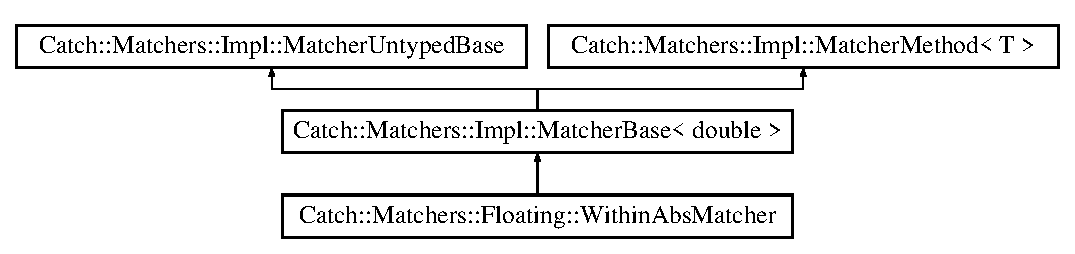
\includegraphics[height=2.968198cm]{struct_catch_1_1_matchers_1_1_floating_1_1_within_abs_matcher}
\end{center}
\end{figure}
\subsection*{Public Member Functions}
\begin{DoxyCompactItemize}
\item 
\mbox{\Hypertarget{struct_catch_1_1_matchers_1_1_floating_1_1_within_abs_matcher_ac45340b98c41230a7def5bd86c2d870f}\label{struct_catch_1_1_matchers_1_1_floating_1_1_within_abs_matcher_ac45340b98c41230a7def5bd86c2d870f}} 
{\bfseries Within\+Abs\+Matcher} (double target, double margin)
\item 
\mbox{\Hypertarget{struct_catch_1_1_matchers_1_1_floating_1_1_within_abs_matcher_afa5d8eed57f12c1e5d006471eb0bfe72}\label{struct_catch_1_1_matchers_1_1_floating_1_1_within_abs_matcher_afa5d8eed57f12c1e5d006471eb0bfe72}} 
bool {\bfseries match} (double const \&matchee) const override
\item 
\mbox{\Hypertarget{struct_catch_1_1_matchers_1_1_floating_1_1_within_abs_matcher_a206a738680f8767af31d3f1835afff3f}\label{struct_catch_1_1_matchers_1_1_floating_1_1_within_abs_matcher_a206a738680f8767af31d3f1835afff3f}} 
std\+::string {\bfseries describe} () const override
\end{DoxyCompactItemize}
\subsection*{Additional Inherited Members}


The documentation for this struct was generated from the following file\+:\begin{DoxyCompactItemize}
\item 
D\+:/kouluhommat/\+Advanced Object-\/\+Oriented Programming/lopputyö/\+Battleship/\+Battleship/catch.\+hpp\end{DoxyCompactItemize}

\hypertarget{struct_catch_1_1_matchers_1_1_floating_1_1_within_ulps_matcher}{}\section{Catch\+:\+:Matchers\+:\+:Floating\+:\+:Within\+Ulps\+Matcher Struct Reference}
\label{struct_catch_1_1_matchers_1_1_floating_1_1_within_ulps_matcher}\index{Catch\+::\+Matchers\+::\+Floating\+::\+Within\+Ulps\+Matcher@{Catch\+::\+Matchers\+::\+Floating\+::\+Within\+Ulps\+Matcher}}


{\ttfamily \#include $<$catch.\+hpp$>$}

Inheritance diagram for Catch\+:\+:Matchers\+:\+:Floating\+:\+:Within\+Ulps\+Matcher\+:\begin{figure}[H]
\begin{center}
\leavevmode
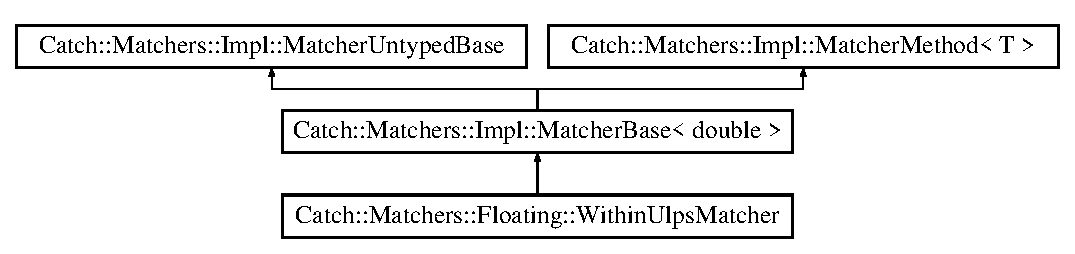
\includegraphics[height=2.968198cm]{struct_catch_1_1_matchers_1_1_floating_1_1_within_ulps_matcher}
\end{center}
\end{figure}
\subsection*{Public Member Functions}
\begin{DoxyCompactItemize}
\item 
\mbox{\hyperlink{struct_catch_1_1_matchers_1_1_floating_1_1_within_ulps_matcher_a836074ae4010275284ab66b2485c6575}{Within\+Ulps\+Matcher}} (double target, int ulps, Floating\+Point\+Kind base\+Type)
\item 
bool \mbox{\hyperlink{struct_catch_1_1_matchers_1_1_floating_1_1_within_ulps_matcher_aabda42a0dc5d00f3c5916feb75006b32}{match}} (double const \&matchee) const override
\item 
std\+::string \mbox{\hyperlink{struct_catch_1_1_matchers_1_1_floating_1_1_within_ulps_matcher_ad9bc8bb7f3abd326580a4bf6cf369b1b}{describe}} () const override
\end{DoxyCompactItemize}
\subsection*{Additional Inherited Members}


\subsection{Constructor \& Destructor Documentation}
\mbox{\Hypertarget{struct_catch_1_1_matchers_1_1_floating_1_1_within_ulps_matcher_a836074ae4010275284ab66b2485c6575}\label{struct_catch_1_1_matchers_1_1_floating_1_1_within_ulps_matcher_a836074ae4010275284ab66b2485c6575}} 
\index{Catch\+::\+Matchers\+::\+Floating\+::\+Within\+Ulps\+Matcher@{Catch\+::\+Matchers\+::\+Floating\+::\+Within\+Ulps\+Matcher}!Within\+Ulps\+Matcher@{Within\+Ulps\+Matcher}}
\index{Within\+Ulps\+Matcher@{Within\+Ulps\+Matcher}!Catch\+::\+Matchers\+::\+Floating\+::\+Within\+Ulps\+Matcher@{Catch\+::\+Matchers\+::\+Floating\+::\+Within\+Ulps\+Matcher}}
\subsubsection{\texorpdfstring{Within\+Ulps\+Matcher()}{WithinUlpsMatcher()}}
{\footnotesize\ttfamily Catch\+::\+Matchers\+::\+Floating\+::\+Within\+Ulps\+Matcher\+::\+Within\+Ulps\+Matcher (\begin{DoxyParamCaption}\item[{double}]{target,  }\item[{int}]{ulps,  }\item[{Floating\+Point\+Kind}]{base\+Type }\end{DoxyParamCaption})}



\subsection{Member Function Documentation}
\mbox{\Hypertarget{struct_catch_1_1_matchers_1_1_floating_1_1_within_ulps_matcher_ad9bc8bb7f3abd326580a4bf6cf369b1b}\label{struct_catch_1_1_matchers_1_1_floating_1_1_within_ulps_matcher_ad9bc8bb7f3abd326580a4bf6cf369b1b}} 
\index{Catch\+::\+Matchers\+::\+Floating\+::\+Within\+Ulps\+Matcher@{Catch\+::\+Matchers\+::\+Floating\+::\+Within\+Ulps\+Matcher}!describe@{describe}}
\index{describe@{describe}!Catch\+::\+Matchers\+::\+Floating\+::\+Within\+Ulps\+Matcher@{Catch\+::\+Matchers\+::\+Floating\+::\+Within\+Ulps\+Matcher}}
\subsubsection{\texorpdfstring{describe()}{describe()}}
{\footnotesize\ttfamily std\+::string Catch\+::\+Matchers\+::\+Floating\+::\+Within\+Ulps\+Matcher\+::describe (\begin{DoxyParamCaption}{ }\end{DoxyParamCaption}) const\hspace{0.3cm}{\ttfamily [override]}, {\ttfamily [virtual]}}



Implements \mbox{\hyperlink{class_catch_1_1_matchers_1_1_impl_1_1_matcher_untyped_base_a91d3a907dbfcbb596077df24f6e11fe2}{Catch\+::\+Matchers\+::\+Impl\+::\+Matcher\+Untyped\+Base}}.

\mbox{\Hypertarget{struct_catch_1_1_matchers_1_1_floating_1_1_within_ulps_matcher_aabda42a0dc5d00f3c5916feb75006b32}\label{struct_catch_1_1_matchers_1_1_floating_1_1_within_ulps_matcher_aabda42a0dc5d00f3c5916feb75006b32}} 
\index{Catch\+::\+Matchers\+::\+Floating\+::\+Within\+Ulps\+Matcher@{Catch\+::\+Matchers\+::\+Floating\+::\+Within\+Ulps\+Matcher}!match@{match}}
\index{match@{match}!Catch\+::\+Matchers\+::\+Floating\+::\+Within\+Ulps\+Matcher@{Catch\+::\+Matchers\+::\+Floating\+::\+Within\+Ulps\+Matcher}}
\subsubsection{\texorpdfstring{match()}{match()}}
{\footnotesize\ttfamily bool Catch\+::\+Matchers\+::\+Floating\+::\+Within\+Ulps\+Matcher\+::match (\begin{DoxyParamCaption}\item[{double const \&}]{matchee }\end{DoxyParamCaption}) const\hspace{0.3cm}{\ttfamily [override]}}



The documentation for this struct was generated from the following file\+:\begin{DoxyCompactItemize}
\item 
D\+:/kouluhommat/\+Advanced Object-\/\+Oriented Programming/lopputyö/\+Battleship/\+Battleship/\mbox{\hyperlink{catch_8hpp}{catch.\+hpp}}\end{DoxyCompactItemize}

\chapter{File Documentation}
\hypertarget{_board_8cpp}{}\section{D\+:/kouluhommat/\+Advanced Object-\/\+Oriented Programming/lopputyö/\+Battleship/\+Battleship/\+Board.cpp File Reference}
\label{_board_8cpp}\index{D\+:/kouluhommat/\+Advanced Object-\/\+Oriented Programming/lopputyö/\+Battleship/\+Battleship/\+Board.\+cpp@{D\+:/kouluhommat/\+Advanced Object-\/\+Oriented Programming/lopputyö/\+Battleship/\+Battleship/\+Board.\+cpp}}


contains implementation for \mbox{\hyperlink{class_board}{Board}} classes  


{\ttfamily \#include \char`\"{}Board.\+h\char`\"{}}\newline
{\ttfamily \#include \char`\"{}Game.\+h\char`\"{}}\newline
{\ttfamily \#include \char`\"{}Globals.\+h\char`\"{}}\newline
{\ttfamily \#include $<$iostream$>$}\newline
\subsection*{Classes}
\begin{DoxyCompactItemize}
\item 
class \mbox{\hyperlink{class_board_impl}{Board\+Impl}}
\end{DoxyCompactItemize}


\subsection{Detailed Description}
contains implementation for \mbox{\hyperlink{class_board}{Board}} classes 


\hypertarget{_board_8h}{}\section{D\+:/kouluhommat/\+Advanced Object-\/\+Oriented Programming/lopputyö/\+Battleship/\+Battleship/\+Board.h File Reference}
\label{_board_8h}\index{D\+:/kouluhommat/\+Advanced Object-\/\+Oriented Programming/lopputyö/\+Battleship/\+Battleship/\+Board.\+h@{D\+:/kouluhommat/\+Advanced Object-\/\+Oriented Programming/lopputyö/\+Battleship/\+Battleship/\+Board.\+h}}


contains header for game board class  


{\ttfamily \#include \char`\"{}Globals.\+h\char`\"{}}\newline
\subsection*{Classes}
\begin{DoxyCompactItemize}
\item 
class \mbox{\hyperlink{class_board}{Board}}
\item 
class \mbox{\hyperlink{class_board_impl}{Board\+Impl}}
\end{DoxyCompactItemize}


\subsection{Detailed Description}
contains header for game board class 


\hypertarget{_board__tests_8cpp}{}\section{D\+:/kouluhommat/\+Advanced Object-\/\+Oriented Programming/lopputyö/\+Battleship/\+Battleship/\+Board\+\_\+tests.cpp File Reference}
\label{_board__tests_8cpp}\index{D\+:/kouluhommat/\+Advanced Object-\/\+Oriented Programming/lopputyö/\+Battleship/\+Battleship/\+Board\+\_\+tests.\+cpp@{D\+:/kouluhommat/\+Advanced Object-\/\+Oriented Programming/lopputyö/\+Battleship/\+Battleship/\+Board\+\_\+tests.\+cpp}}


contains test cases for \mbox{\hyperlink{class_board}{Board}} classes  


{\ttfamily \#include \char`\"{}catch.\+hpp\char`\"{}}\newline
{\ttfamily \#include \char`\"{}Board.\+h\char`\"{}}\newline
{\ttfamily \#include \char`\"{}Game.\+h\char`\"{}}\newline
{\ttfamily \#include \char`\"{}Globals.\+h\char`\"{}}\newline
\subsection*{Macros}
\begin{DoxyCompactItemize}
\item 
\#define \mbox{\hyperlink{_board__tests_8cpp_a656eb5868e824d59f489f910db438420}{C\+A\+T\+C\+H\+\_\+\+C\+O\+N\+F\+I\+G\+\_\+\+M\+A\+IN}}
\end{DoxyCompactItemize}
\subsection*{Functions}
\begin{DoxyCompactItemize}
\item 
\mbox{\hyperlink{_board__tests_8cpp_a4f7046e2aee2066ad4ce8e69249c5d1a}{T\+E\+S\+T\+\_\+\+C\+A\+SE}} (\char`\"{}Board tests\char`\"{}, \char`\"{}\mbox{[}board\mbox{]}\char`\"{})
\end{DoxyCompactItemize}


\subsection{Detailed Description}
contains test cases for \mbox{\hyperlink{class_board}{Board}} classes 



\subsection{Macro Definition Documentation}
\mbox{\Hypertarget{_board__tests_8cpp_a656eb5868e824d59f489f910db438420}\label{_board__tests_8cpp_a656eb5868e824d59f489f910db438420}} 
\index{Board\+\_\+tests.\+cpp@{Board\+\_\+tests.\+cpp}!C\+A\+T\+C\+H\+\_\+\+C\+O\+N\+F\+I\+G\+\_\+\+M\+A\+IN@{C\+A\+T\+C\+H\+\_\+\+C\+O\+N\+F\+I\+G\+\_\+\+M\+A\+IN}}
\index{C\+A\+T\+C\+H\+\_\+\+C\+O\+N\+F\+I\+G\+\_\+\+M\+A\+IN@{C\+A\+T\+C\+H\+\_\+\+C\+O\+N\+F\+I\+G\+\_\+\+M\+A\+IN}!Board\+\_\+tests.\+cpp@{Board\+\_\+tests.\+cpp}}
\subsubsection{\texorpdfstring{C\+A\+T\+C\+H\+\_\+\+C\+O\+N\+F\+I\+G\+\_\+\+M\+A\+IN}{CATCH\_CONFIG\_MAIN}}
{\footnotesize\ttfamily \#define C\+A\+T\+C\+H\+\_\+\+C\+O\+N\+F\+I\+G\+\_\+\+M\+A\+IN}



\subsection{Function Documentation}
\mbox{\Hypertarget{_board__tests_8cpp_a4f7046e2aee2066ad4ce8e69249c5d1a}\label{_board__tests_8cpp_a4f7046e2aee2066ad4ce8e69249c5d1a}} 
\index{Board\+\_\+tests.\+cpp@{Board\+\_\+tests.\+cpp}!T\+E\+S\+T\+\_\+\+C\+A\+SE@{T\+E\+S\+T\+\_\+\+C\+A\+SE}}
\index{T\+E\+S\+T\+\_\+\+C\+A\+SE@{T\+E\+S\+T\+\_\+\+C\+A\+SE}!Board\+\_\+tests.\+cpp@{Board\+\_\+tests.\+cpp}}
\subsubsection{\texorpdfstring{T\+E\+S\+T\+\_\+\+C\+A\+S\+E()}{TEST\_CASE()}}
{\footnotesize\ttfamily T\+E\+S\+T\+\_\+\+C\+A\+SE (\begin{DoxyParamCaption}\item[{\char`\"{}Board tests\char`\"{}}]{,  }\item[{\char`\"{}\char`\"{}}]{\mbox{[}board\mbox{]} }\end{DoxyParamCaption})}


\hypertarget{_board_impl_8cpp}{}\section{D\+:/kouluhommat/\+Advanced Object-\/\+Oriented Programming/lopputyö/\+Battleship/\+Battleship/\+Board\+Impl.cpp File Reference}
\label{_board_impl_8cpp}\index{D\+:/kouluhommat/\+Advanced Object-\/\+Oriented Programming/lopputyö/\+Battleship/\+Battleship/\+Board\+Impl.\+cpp@{D\+:/kouluhommat/\+Advanced Object-\/\+Oriented Programming/lopputyö/\+Battleship/\+Battleship/\+Board\+Impl.\+cpp}}


contains implementation for \mbox{\hyperlink{class_board}{Board}} classes and assisting functions  


{\ttfamily \#include \char`\"{}Board.\+h\char`\"{}}\newline
{\ttfamily \#include \char`\"{}Game.\+h\char`\"{}}\newline
{\ttfamily \#include \char`\"{}Globals.\+h\char`\"{}}\newline
{\ttfamily \#include $<$iostream$>$}\newline


\subsection{Detailed Description}
contains implementation for \mbox{\hyperlink{class_board}{Board}} classes and assisting functions 


\hypertarget{_board_impl_8h}{}\section{D\+:/kouluhommat/\+Advanced Object-\/\+Oriented Programming/lopputyö/\+Battleship/\+Battleship/\+Board\+Impl.h File Reference}
\label{_board_impl_8h}\index{D\+:/kouluhommat/\+Advanced Object-\/\+Oriented Programming/lopputyö/\+Battleship/\+Battleship/\+Board\+Impl.\+h@{D\+:/kouluhommat/\+Advanced Object-\/\+Oriented Programming/lopputyö/\+Battleship/\+Battleship/\+Board\+Impl.\+h}}


contains header for game board implementation class  


{\ttfamily \#include \char`\"{}Globals.\+h\char`\"{}}\newline
\subsection*{Classes}
\begin{DoxyCompactItemize}
\item 
class \mbox{\hyperlink{class_board_impl}{Board\+Impl}}
\end{DoxyCompactItemize}


\subsection{Detailed Description}
contains header for game board implementation class 


\hypertarget{_easy_player_8h}{}\section{D\+:/kouluhommat/\+Advanced Object-\/\+Oriented Programming/lopputyö/\+Battleship/\+Battleship/\+Easy\+Player.h File Reference}
\label{_easy_player_8h}\index{D\+:/kouluhommat/\+Advanced Object-\/\+Oriented Programming/lopputyö/\+Battleship/\+Battleship/\+Easy\+Player.\+h@{D\+:/kouluhommat/\+Advanced Object-\/\+Oriented Programming/lopputyö/\+Battleship/\+Battleship/\+Easy\+Player.\+h}}


contains header for easy player class  


{\ttfamily \#include \char`\"{}Player.\+h\char`\"{}}\newline
\subsection*{Classes}
\begin{DoxyCompactItemize}
\item 
class \mbox{\hyperlink{class_easy_player}{Easy\+Player}}
\end{DoxyCompactItemize}


\subsection{Detailed Description}
contains header for easy player class 


\hypertarget{_game_8cpp}{}\section{D\+:/kouluhommat/\+Advanced Object-\/\+Oriented Programming/lopputyö/\+Battleship/\+Battleship/\+Game.cpp File Reference}
\label{_game_8cpp}\index{D\+:/kouluhommat/\+Advanced Object-\/\+Oriented Programming/lopputyö/\+Battleship/\+Battleship/\+Game.\+cpp@{D\+:/kouluhommat/\+Advanced Object-\/\+Oriented Programming/lopputyö/\+Battleship/\+Battleship/\+Game.\+cpp}}


contains implementation for \mbox{\hyperlink{class_game}{Game}} classes and assisting functions  


{\ttfamily \#include \char`\"{}Game.\+h\char`\"{}}\newline
{\ttfamily \#include \char`\"{}Board.\+h\char`\"{}}\newline
{\ttfamily \#include \char`\"{}Player.\+h\char`\"{}}\newline
{\ttfamily \#include \char`\"{}Globals.\+h\char`\"{}}\newline
{\ttfamily \#include \char`\"{}Ship.\+h\char`\"{}}\newline
{\ttfamily \#include $<$iostream$>$}\newline
{\ttfamily \#include $<$string$>$}\newline
{\ttfamily \#include $<$cstdlib$>$}\newline
{\ttfamily \#include $<$cctype$>$}\newline
{\ttfamily \#include $<$vector$>$}\newline
{\ttfamily \#include $<$algorithm$>$}\newline
\subsection*{Classes}
\begin{DoxyCompactItemize}
\item 
class \mbox{\hyperlink{class_game_impl}{Game\+Impl}}
\end{DoxyCompactItemize}
\subsection*{Functions}
\begin{DoxyCompactItemize}
\item 
void \mbox{\hyperlink{_game_8cpp_aa3b21853f890838c88d047d6c2786917}{wait}} ()
\end{DoxyCompactItemize}


\subsection{Detailed Description}
contains implementation for \mbox{\hyperlink{class_game}{Game}} classes and assisting functions 



\subsection{Function Documentation}
\mbox{\Hypertarget{_game_8cpp_aa3b21853f890838c88d047d6c2786917}\label{_game_8cpp_aa3b21853f890838c88d047d6c2786917}} 
\index{Game.\+cpp@{Game.\+cpp}!wait@{wait}}
\index{wait@{wait}!Game.\+cpp@{Game.\+cpp}}
\subsubsection{\texorpdfstring{wait()}{wait()}}
{\footnotesize\ttfamily void wait (\begin{DoxyParamCaption}{ }\end{DoxyParamCaption})}

Function for pausing the game 
\hypertarget{_game_8h}{}\section{D\+:/kouluhommat/\+Advanced Object-\/\+Oriented Programming/lopputyö/\+Battleship/\+Battleship/\+Game.h File Reference}
\label{_game_8h}\index{D\+:/kouluhommat/\+Advanced Object-\/\+Oriented Programming/lopputyö/\+Battleship/\+Battleship/\+Game.\+h@{D\+:/kouluhommat/\+Advanced Object-\/\+Oriented Programming/lopputyö/\+Battleship/\+Battleship/\+Game.\+h}}


contains header for \mbox{\hyperlink{class_game}{Game}} class  


{\ttfamily \#include \char`\"{}Board.\+h\char`\"{}}\newline
{\ttfamily \#include \char`\"{}Ship.\+h\char`\"{}}\newline
{\ttfamily \#include $<$string$>$}\newline
{\ttfamily \#include $<$cassert$>$}\newline
\subsection*{Classes}
\begin{DoxyCompactItemize}
\item 
class \mbox{\hyperlink{class_game}{Game}}
\begin{DoxyCompactList}\small\item\em Declaration for game implementation class. \end{DoxyCompactList}\item 
class \mbox{\hyperlink{class_game_impl}{Game\+Impl}}
\end{DoxyCompactItemize}


\subsection{Detailed Description}
contains header for \mbox{\hyperlink{class_game}{Game}} class 


\hypertarget{_game__tests_8cpp}{}\section{D\+:/kouluhommat/\+Advanced Object-\/\+Oriented Programming/lopputyö/\+Battleship/\+Battleship/\+Game\+\_\+tests.cpp File Reference}
\label{_game__tests_8cpp}\index{D\+:/kouluhommat/\+Advanced Object-\/\+Oriented Programming/lopputyö/\+Battleship/\+Battleship/\+Game\+\_\+tests.\+cpp@{D\+:/kouluhommat/\+Advanced Object-\/\+Oriented Programming/lopputyö/\+Battleship/\+Battleship/\+Game\+\_\+tests.\+cpp}}


contains test cases for game class  


{\ttfamily \#include \char`\"{}catch.\+hpp\char`\"{}}\newline
{\ttfamily \#include \char`\"{}Game.\+h\char`\"{}}\newline
{\ttfamily \#include \char`\"{}Board.\+h\char`\"{}}\newline
{\ttfamily \#include \char`\"{}Player.\+h\char`\"{}}\newline
{\ttfamily \#include \char`\"{}Globals.\+h\char`\"{}}\newline
\subsection*{Macros}
\begin{DoxyCompactItemize}
\item 
\#define \mbox{\hyperlink{_game__tests_8cpp_a656eb5868e824d59f489f910db438420}{C\+A\+T\+C\+H\+\_\+\+C\+O\+N\+F\+I\+G\+\_\+\+M\+A\+IN}}
\end{DoxyCompactItemize}
\subsection*{Functions}
\begin{DoxyCompactItemize}
\item 
\mbox{\hyperlink{_game__tests_8cpp_a06a5d13540cb9bda057ea077c55403b0}{T\+E\+S\+T\+\_\+\+C\+A\+SE}} (\char`\"{}Game tests\char`\"{}, \char`\"{}\mbox{[}game\mbox{]}\char`\"{})
\end{DoxyCompactItemize}


\subsection{Detailed Description}
contains test cases for game class 



\subsection{Macro Definition Documentation}
\mbox{\Hypertarget{_game__tests_8cpp_a656eb5868e824d59f489f910db438420}\label{_game__tests_8cpp_a656eb5868e824d59f489f910db438420}} 
\index{Game\+\_\+tests.\+cpp@{Game\+\_\+tests.\+cpp}!C\+A\+T\+C\+H\+\_\+\+C\+O\+N\+F\+I\+G\+\_\+\+M\+A\+IN@{C\+A\+T\+C\+H\+\_\+\+C\+O\+N\+F\+I\+G\+\_\+\+M\+A\+IN}}
\index{C\+A\+T\+C\+H\+\_\+\+C\+O\+N\+F\+I\+G\+\_\+\+M\+A\+IN@{C\+A\+T\+C\+H\+\_\+\+C\+O\+N\+F\+I\+G\+\_\+\+M\+A\+IN}!Game\+\_\+tests.\+cpp@{Game\+\_\+tests.\+cpp}}
\subsubsection{\texorpdfstring{C\+A\+T\+C\+H\+\_\+\+C\+O\+N\+F\+I\+G\+\_\+\+M\+A\+IN}{CATCH\_CONFIG\_MAIN}}
{\footnotesize\ttfamily \#define C\+A\+T\+C\+H\+\_\+\+C\+O\+N\+F\+I\+G\+\_\+\+M\+A\+IN}



\subsection{Function Documentation}
\mbox{\Hypertarget{_game__tests_8cpp_a06a5d13540cb9bda057ea077c55403b0}\label{_game__tests_8cpp_a06a5d13540cb9bda057ea077c55403b0}} 
\index{Game\+\_\+tests.\+cpp@{Game\+\_\+tests.\+cpp}!T\+E\+S\+T\+\_\+\+C\+A\+SE@{T\+E\+S\+T\+\_\+\+C\+A\+SE}}
\index{T\+E\+S\+T\+\_\+\+C\+A\+SE@{T\+E\+S\+T\+\_\+\+C\+A\+SE}!Game\+\_\+tests.\+cpp@{Game\+\_\+tests.\+cpp}}
\subsubsection{\texorpdfstring{T\+E\+S\+T\+\_\+\+C\+A\+S\+E()}{TEST\_CASE()}}
{\footnotesize\ttfamily T\+E\+S\+T\+\_\+\+C\+A\+SE (\begin{DoxyParamCaption}\item[{\char`\"{}Game tests\char`\"{}}]{,  }\item[{\char`\"{}\char`\"{}}]{\mbox{[}game\mbox{]} }\end{DoxyParamCaption})}


\hypertarget{_game_impl_8cpp}{}\section{D\+:/kouluhommat/\+Advanced Object-\/\+Oriented Programming/lopputyö/\+Battleship/\+Battleship/\+Game\+Impl.cpp File Reference}
\label{_game_impl_8cpp}\index{D\+:/kouluhommat/\+Advanced Object-\/\+Oriented Programming/lopputyö/\+Battleship/\+Battleship/\+Game\+Impl.\+cpp@{D\+:/kouluhommat/\+Advanced Object-\/\+Oriented Programming/lopputyö/\+Battleship/\+Battleship/\+Game\+Impl.\+cpp}}


contains implementation for \mbox{\hyperlink{class_game}{Game}} classes and assisting functions  


{\ttfamily \#include \char`\"{}Game\+Impl.\+h\char`\"{}}\newline
{\ttfamily \#include \char`\"{}Player.\+h\char`\"{}}\newline
{\ttfamily \#include \char`\"{}Globals.\+h\char`\"{}}\newline
{\ttfamily \#include $<$iostream$>$}\newline
{\ttfamily \#include $<$string$>$}\newline
{\ttfamily \#include $<$cstdlib$>$}\newline
{\ttfamily \#include $<$cctype$>$}\newline
{\ttfamily \#include $<$vector$>$}\newline
{\ttfamily \#include $<$algorithm$>$}\newline
\subsection*{Functions}
\begin{DoxyCompactItemize}
\item 
void \mbox{\hyperlink{_game_impl_8cpp_aa3b21853f890838c88d047d6c2786917}{wait}} ()
\end{DoxyCompactItemize}


\subsection{Detailed Description}
contains implementation for \mbox{\hyperlink{class_game}{Game}} classes and assisting functions 



\subsection{Function Documentation}
\mbox{\Hypertarget{_game_impl_8cpp_aa3b21853f890838c88d047d6c2786917}\label{_game_impl_8cpp_aa3b21853f890838c88d047d6c2786917}} 
\index{Game\+Impl.\+cpp@{Game\+Impl.\+cpp}!wait@{wait}}
\index{wait@{wait}!Game\+Impl.\+cpp@{Game\+Impl.\+cpp}}
\subsubsection{\texorpdfstring{wait()}{wait()}}
{\footnotesize\ttfamily void wait (\begin{DoxyParamCaption}{ }\end{DoxyParamCaption})}

Function for pausing the game 
\hypertarget{_game_impl_8h}{}\section{D\+:/kouluhommat/\+Advanced Object-\/\+Oriented Programming/lopputyö/\+Battleship/\+Battleship/\+Game\+Impl.h File Reference}
\label{_game_impl_8h}\index{D\+:/kouluhommat/\+Advanced Object-\/\+Oriented Programming/lopputyö/\+Battleship/\+Battleship/\+Game\+Impl.\+h@{D\+:/kouluhommat/\+Advanced Object-\/\+Oriented Programming/lopputyö/\+Battleship/\+Battleship/\+Game\+Impl.\+h}}


contains header for \mbox{\hyperlink{class_game}{Game}} implementation class  


{\ttfamily \#include \char`\"{}Board.\+h\char`\"{}}\newline
{\ttfamily \#include \char`\"{}Ship.\+h\char`\"{}}\newline
{\ttfamily \#include $<$string$>$}\newline
{\ttfamily \#include $<$cassert$>$}\newline
\subsection*{Classes}
\begin{DoxyCompactItemize}
\item 
class \mbox{\hyperlink{class_game_impl}{Game\+Impl}}
\begin{DoxyCompactList}\small\item\em Declaration for \mbox{\hyperlink{class_player}{Player}} class. \end{DoxyCompactList}\end{DoxyCompactItemize}


\subsection{Detailed Description}
contains header for \mbox{\hyperlink{class_game}{Game}} implementation class 


\hypertarget{_globals_8h}{}\section{D\+:/kouluhommat/\+Advanced Object-\/\+Oriented Programming/lopputyö/\+Battleship/\+Battleship/\+Globals.h File Reference}
\label{_globals_8h}\index{D\+:/kouluhommat/\+Advanced Object-\/\+Oriented Programming/lopputyö/\+Battleship/\+Battleship/\+Globals.\+h@{D\+:/kouluhommat/\+Advanced Object-\/\+Oriented Programming/lopputyö/\+Battleship/\+Battleship/\+Globals.\+h}}


contains header for global classes and functions  


{\ttfamily \#include $<$random$>$}\newline
\subsection*{Classes}
\begin{DoxyCompactItemize}
\item 
class \mbox{\hyperlink{class_point}{Point}}
\end{DoxyCompactItemize}
\subsection*{Enumerations}
\begin{DoxyCompactItemize}
\item 
enum \mbox{\hyperlink{_globals_8h_a224b9163917ac32fc95a60d8c1eec3aa}{Direction}} \{ \mbox{\hyperlink{_globals_8h_a224b9163917ac32fc95a60d8c1eec3aaa4dd51ad73508d6fc83a502966779e48e}{H\+O\+R\+I\+Z\+O\+N\+T\+AL}}, 
\mbox{\hyperlink{_globals_8h_a224b9163917ac32fc95a60d8c1eec3aaa1a88641fcd39f2ed3e58a18526e97138}{V\+E\+R\+T\+I\+C\+AL}}
 \}
\begin{DoxyCompactList}\small\item\em Enumeration for ship\textquotesingle{}s direction. \end{DoxyCompactList}\end{DoxyCompactItemize}
\subsection*{Functions}
\begin{DoxyCompactItemize}
\item 
int \mbox{\hyperlink{_globals_8h_a96fd653a75890268fa4616e1c6442343}{random\+Int}} (int limit)
\end{DoxyCompactItemize}
\subsection*{Variables}
\begin{DoxyCompactItemize}
\item 
const int \mbox{\hyperlink{_globals_8h_ad49ec6ee42a33fd302462b66950529ed}{M\+A\+X\+R\+O\+WS}} = 10
\begin{DoxyCompactList}\small\item\em Integer for maximum rows. \end{DoxyCompactList}\item 
const int \mbox{\hyperlink{_globals_8h_a9b3ce626f4086356c27a53d28043199c}{M\+A\+X\+C\+O\+LS}} = 10
\begin{DoxyCompactList}\small\item\em Integer for maximum columns. \end{DoxyCompactList}\end{DoxyCompactItemize}


\subsection{Detailed Description}
contains header for global classes and functions 



\subsection{Enumeration Type Documentation}
\mbox{\Hypertarget{_globals_8h_a224b9163917ac32fc95a60d8c1eec3aa}\label{_globals_8h_a224b9163917ac32fc95a60d8c1eec3aa}} 
\index{Globals.\+h@{Globals.\+h}!Direction@{Direction}}
\index{Direction@{Direction}!Globals.\+h@{Globals.\+h}}
\subsubsection{\texorpdfstring{Direction}{Direction}}
{\footnotesize\ttfamily enum \mbox{\hyperlink{_globals_8h_a224b9163917ac32fc95a60d8c1eec3aa}{Direction}}}



Enumeration for ship\textquotesingle{}s direction. 

\begin{DoxyEnumFields}{Enumerator}
\raisebox{\heightof{T}}[0pt][0pt]{\index{H\+O\+R\+I\+Z\+O\+N\+T\+AL@{H\+O\+R\+I\+Z\+O\+N\+T\+AL}!Globals.\+h@{Globals.\+h}}\index{Globals.\+h@{Globals.\+h}!H\+O\+R\+I\+Z\+O\+N\+T\+AL@{H\+O\+R\+I\+Z\+O\+N\+T\+AL}}}\mbox{\Hypertarget{_globals_8h_a224b9163917ac32fc95a60d8c1eec3aaa4dd51ad73508d6fc83a502966779e48e}\label{_globals_8h_a224b9163917ac32fc95a60d8c1eec3aaa4dd51ad73508d6fc83a502966779e48e}} 
H\+O\+R\+I\+Z\+O\+N\+T\+AL&\\
\hline

\raisebox{\heightof{T}}[0pt][0pt]{\index{V\+E\+R\+T\+I\+C\+AL@{V\+E\+R\+T\+I\+C\+AL}!Globals.\+h@{Globals.\+h}}\index{Globals.\+h@{Globals.\+h}!V\+E\+R\+T\+I\+C\+AL@{V\+E\+R\+T\+I\+C\+AL}}}\mbox{\Hypertarget{_globals_8h_a224b9163917ac32fc95a60d8c1eec3aaa1a88641fcd39f2ed3e58a18526e97138}\label{_globals_8h_a224b9163917ac32fc95a60d8c1eec3aaa1a88641fcd39f2ed3e58a18526e97138}} 
V\+E\+R\+T\+I\+C\+AL&\\
\hline

\end{DoxyEnumFields}


\subsection{Function Documentation}
\mbox{\Hypertarget{_globals_8h_a96fd653a75890268fa4616e1c6442343}\label{_globals_8h_a96fd653a75890268fa4616e1c6442343}} 
\index{Globals.\+h@{Globals.\+h}!random\+Int@{random\+Int}}
\index{random\+Int@{random\+Int}!Globals.\+h@{Globals.\+h}}
\subsubsection{\texorpdfstring{random\+Int()}{randomInt()}}
{\footnotesize\ttfamily int random\+Int (\begin{DoxyParamCaption}\item[{int}]{limit }\end{DoxyParamCaption})\hspace{0.3cm}{\ttfamily [inline]}}

Function for getting random integer 
\begin{DoxyParams}{Parameters}
{\em limit} & integer containing upper limit of the randomized number \\
\hline
\end{DoxyParams}
$<$ Creates a random device

$<$ Creates a Mersenne twister 19937 generator

$<$ Produces random int in a range 

\subsection{Variable Documentation}
\mbox{\Hypertarget{_globals_8h_a9b3ce626f4086356c27a53d28043199c}\label{_globals_8h_a9b3ce626f4086356c27a53d28043199c}} 
\index{Globals.\+h@{Globals.\+h}!M\+A\+X\+C\+O\+LS@{M\+A\+X\+C\+O\+LS}}
\index{M\+A\+X\+C\+O\+LS@{M\+A\+X\+C\+O\+LS}!Globals.\+h@{Globals.\+h}}
\subsubsection{\texorpdfstring{M\+A\+X\+C\+O\+LS}{MAXCOLS}}
{\footnotesize\ttfamily const int M\+A\+X\+C\+O\+LS = 10}



Integer for maximum columns. 

\mbox{\Hypertarget{_globals_8h_ad49ec6ee42a33fd302462b66950529ed}\label{_globals_8h_ad49ec6ee42a33fd302462b66950529ed}} 
\index{Globals.\+h@{Globals.\+h}!M\+A\+X\+R\+O\+WS@{M\+A\+X\+R\+O\+WS}}
\index{M\+A\+X\+R\+O\+WS@{M\+A\+X\+R\+O\+WS}!Globals.\+h@{Globals.\+h}}
\subsubsection{\texorpdfstring{M\+A\+X\+R\+O\+WS}{MAXROWS}}
{\footnotesize\ttfamily const int M\+A\+X\+R\+O\+WS = 10}



Integer for maximum rows. 


\hypertarget{_hard_player_8h}{}\section{D\+:/kouluhommat/\+Advanced Object-\/\+Oriented Programming/lopputyö/\+Battleship/\+Battleship/\+Hard\+Player.h File Reference}
\label{_hard_player_8h}\index{D\+:/kouluhommat/\+Advanced Object-\/\+Oriented Programming/lopputyö/\+Battleship/\+Battleship/\+Hard\+Player.\+h@{D\+:/kouluhommat/\+Advanced Object-\/\+Oriented Programming/lopputyö/\+Battleship/\+Battleship/\+Hard\+Player.\+h}}


contains header for hard player class  


{\ttfamily \#include \char`\"{}Player.\+h\char`\"{}}\newline
\subsection*{Classes}
\begin{DoxyCompactItemize}
\item 
class \mbox{\hyperlink{class_hard_player}{Hard\+Player}}
\end{DoxyCompactItemize}


\subsection{Detailed Description}
contains header for hard player class 


\hypertarget{_human_player_8h}{}\section{D\+:/kouluhommat/\+Advanced Object-\/\+Oriented Programming/lopputyö/\+Battleship/\+Battleship/\+Human\+Player.h File Reference}
\label{_human_player_8h}\index{D\+:/kouluhommat/\+Advanced Object-\/\+Oriented Programming/lopputyö/\+Battleship/\+Battleship/\+Human\+Player.\+h@{D\+:/kouluhommat/\+Advanced Object-\/\+Oriented Programming/lopputyö/\+Battleship/\+Battleship/\+Human\+Player.\+h}}


contains header for human player class  


{\ttfamily \#include \char`\"{}Player.\+h\char`\"{}}\newline
\subsection*{Classes}
\begin{DoxyCompactItemize}
\item 
class \mbox{\hyperlink{class_human_player}{Human\+Player}}
\end{DoxyCompactItemize}


\subsection{Detailed Description}
contains header for human player class 


\hypertarget{_main_8cpp}{}\section{D\+:/kouluhommat/\+Advanced Object-\/\+Oriented Programming/lopputyö/\+Battleship/\+Battleship/\+Main.cpp File Reference}
\label{_main_8cpp}\index{D\+:/kouluhommat/\+Advanced Object-\/\+Oriented Programming/lopputyö/\+Battleship/\+Battleship/\+Main.\+cpp@{D\+:/kouluhommat/\+Advanced Object-\/\+Oriented Programming/lopputyö/\+Battleship/\+Battleship/\+Main.\+cpp}}


contains Main function of the program with assisting functions  


{\ttfamily \#include \char`\"{}Game.\+h\char`\"{}}\newline
{\ttfamily \#include \char`\"{}Player.\+h\char`\"{}}\newline
{\ttfamily \#include $<$iostream$>$}\newline
{\ttfamily \#include $<$string$>$}\newline
{\ttfamily \#include $<$cassert$>$}\newline
\subsection*{Functions}
\begin{DoxyCompactItemize}
\item 
bool \mbox{\hyperlink{_main_8cpp_ac76b0229964cc6dc169aa5a2f1388ff7}{add\+Ships}} (\mbox{\hyperlink{class_game}{Game}} \&g)
\item 
int \mbox{\hyperlink{_main_8cpp_a34f202909819f5d93192830d691e7a7b}{select\+Bot}} ()
\item 
int \mbox{\hyperlink{_main_8cpp_ae66f6b31b5ad750f1fe042a706a4e3d4}{main}} ()
\end{DoxyCompactItemize}


\subsection{Detailed Description}
contains Main function of the program with assisting functions 



\subsection{Function Documentation}
\mbox{\Hypertarget{_main_8cpp_ac76b0229964cc6dc169aa5a2f1388ff7}\label{_main_8cpp_ac76b0229964cc6dc169aa5a2f1388ff7}} 
\index{Main.\+cpp@{Main.\+cpp}!add\+Ships@{add\+Ships}}
\index{add\+Ships@{add\+Ships}!Main.\+cpp@{Main.\+cpp}}
\subsubsection{\texorpdfstring{add\+Ships()}{addShips()}}
{\footnotesize\ttfamily bool add\+Ships (\begin{DoxyParamCaption}\item[{\mbox{\hyperlink{class_game}{Game}} \&}]{g }\end{DoxyParamCaption})}

Adds all the ships into the game 
\begin{DoxyParams}{Parameters}
{\em g} & reference to game object \\
\hline
\end{DoxyParams}
\mbox{\Hypertarget{_main_8cpp_ae66f6b31b5ad750f1fe042a706a4e3d4}\label{_main_8cpp_ae66f6b31b5ad750f1fe042a706a4e3d4}} 
\index{Main.\+cpp@{Main.\+cpp}!main@{main}}
\index{main@{main}!Main.\+cpp@{Main.\+cpp}}
\subsubsection{\texorpdfstring{main()}{main()}}
{\footnotesize\ttfamily int main (\begin{DoxyParamCaption}{ }\end{DoxyParamCaption})}

Main function of the program $<$ Creates a game object

Prints game modes for player

Checks if player selected Human vs Human

Creates pointers into player objects

$<$ Adds ships into the game

$<$ Starts game

Deletes players

$<$ Checks if player selected Human vs Bot

$<$ Asks user for bot difficulty ~\newline
~\newline
~\newline
~\newline
~\newline
~\newline
~\newline
~\newline
~\newline
~\newline
~\newline
~\newline
~\newline
~\newline
~\newline
~\newline
~\newline
~\newline
~\newline
~\newline
~\newline
 Checks if bot difficulty is easy

Creates pointers into player objects

$<$ Adds ships into the game

$<$ Starts game

Deletes players

$<$ Checks if bot difficulty is medium ~\newline
~\newline
~\newline
~\newline
~\newline
~\newline
~\newline
~\newline
~\newline
~\newline
~\newline
~\newline
~\newline
~\newline
~\newline
 Creates pointers into player objects

$<$ Adds ships into the game

$<$ Starts game

Deletes players

$<$ Checks if bot difficulty is hard ~\newline
~\newline
~\newline
~\newline
~\newline
~\newline
~\newline
~\newline
~\newline
~\newline
 Creates pointers player objects

$<$ Adds ships into the game

$<$ Starts game

Deletes players

$<$ Checks if player selected Medium\+Bot vs Hard\+Bot ~\newline
~\newline
~\newline
~\newline
~\newline
 Creates pointers into player objects

$<$ Adds ships into the game

$<$ Starts game

Deletes players

$<$ Else choice was invalid \mbox{\Hypertarget{_main_8cpp_a34f202909819f5d93192830d691e7a7b}\label{_main_8cpp_a34f202909819f5d93192830d691e7a7b}} 
\index{Main.\+cpp@{Main.\+cpp}!select\+Bot@{select\+Bot}}
\index{select\+Bot@{select\+Bot}!Main.\+cpp@{Main.\+cpp}}
\subsubsection{\texorpdfstring{select\+Bot()}{selectBot()}}
{\footnotesize\ttfamily int select\+Bot (\begin{DoxyParamCaption}{ }\end{DoxyParamCaption})}

Function for selecting bot difficulty 
\hypertarget{_medium_player_8h}{}\section{D\+:/kouluhommat/\+Advanced Object-\/\+Oriented Programming/lopputyö/\+Battleship/\+Battleship/\+Medium\+Player.h File Reference}
\label{_medium_player_8h}\index{D\+:/kouluhommat/\+Advanced Object-\/\+Oriented Programming/lopputyö/\+Battleship/\+Battleship/\+Medium\+Player.\+h@{D\+:/kouluhommat/\+Advanced Object-\/\+Oriented Programming/lopputyö/\+Battleship/\+Battleship/\+Medium\+Player.\+h}}


contains header for medium player class  


{\ttfamily \#include \char`\"{}Player.\+h\char`\"{}}\newline
\subsection*{Classes}
\begin{DoxyCompactItemize}
\item 
class \mbox{\hyperlink{class_medium_player}{Medium\+Player}}
\end{DoxyCompactItemize}


\subsection{Detailed Description}
contains header for medium player class 


\hypertarget{_player_8cpp}{}\section{D\+:/kouluhommat/\+Advanced Object-\/\+Oriented Programming/lopputyö/\+Battleship/\+Battleship/\+Player.cpp File Reference}
\label{_player_8cpp}\index{D\+:/kouluhommat/\+Advanced Object-\/\+Oriented Programming/lopputyö/\+Battleship/\+Battleship/\+Player.\+cpp@{D\+:/kouluhommat/\+Advanced Object-\/\+Oriented Programming/lopputyö/\+Battleship/\+Battleship/\+Player.\+cpp}}


contains implementation for \mbox{\hyperlink{class_player}{Player}} classes and assisting functions  


{\ttfamily \#include \char`\"{}Player.\+h\char`\"{}}\newline
{\ttfamily \#include \char`\"{}Human\+Player.\+h\char`\"{}}\newline
{\ttfamily \#include \char`\"{}Easy\+Player.\+h\char`\"{}}\newline
{\ttfamily \#include \char`\"{}Medium\+Player.\+h\char`\"{}}\newline
{\ttfamily \#include \char`\"{}Hard\+Player.\+h\char`\"{}}\newline
{\ttfamily \#include $<$iostream$>$}\newline
{\ttfamily \#include $<$string$>$}\newline
{\ttfamily \#include $<$vector$>$}\newline
\subsection*{Functions}
\begin{DoxyCompactItemize}
\item 
bool \mbox{\hyperlink{_player_8cpp_a72b0e7e7c053e4606495cd4c782504f4}{get\+Two\+Integers}} (int \&r, int \&c)
\end{DoxyCompactItemize}


\subsection{Detailed Description}
contains implementation for \mbox{\hyperlink{class_player}{Player}} classes and assisting functions 



\subsection{Function Documentation}
\mbox{\Hypertarget{_player_8cpp_a72b0e7e7c053e4606495cd4c782504f4}\label{_player_8cpp_a72b0e7e7c053e4606495cd4c782504f4}} 
\index{Player.\+cpp@{Player.\+cpp}!get\+Two\+Integers@{get\+Two\+Integers}}
\index{get\+Two\+Integers@{get\+Two\+Integers}!Player.\+cpp@{Player.\+cpp}}
\subsubsection{\texorpdfstring{get\+Two\+Integers()}{getTwoIntegers()}}
{\footnotesize\ttfamily bool get\+Two\+Integers (\begin{DoxyParamCaption}\item[{int \&}]{r,  }\item[{int \&}]{c }\end{DoxyParamCaption})}

Function for getting two integers from user input 
\begin{DoxyParams}{Parameters}
{\em r} & reference to row \\
\hline
{\em c} & reference to column \\
\hline
\end{DoxyParams}
$<$ Checks if result isn\textquotesingle{}t valid

$<$ Clear error state so can\textquotesingle{}t do more input operations 
\hypertarget{_player_8h}{}\section{D\+:/kouluhommat/\+Advanced Object-\/\+Oriented Programming/lopputyö/\+Battleship/\+Battleship/\+Player.h File Reference}
\label{_player_8h}\index{D\+:/kouluhommat/\+Advanced Object-\/\+Oriented Programming/lopputyö/\+Battleship/\+Battleship/\+Player.\+h@{D\+:/kouluhommat/\+Advanced Object-\/\+Oriented Programming/lopputyö/\+Battleship/\+Battleship/\+Player.\+h}}


contains header for player classes  


{\ttfamily \#include \char`\"{}Board.\+h\char`\"{}}\newline
{\ttfamily \#include \char`\"{}Game.\+h\char`\"{}}\newline
\subsection*{Classes}
\begin{DoxyCompactItemize}
\item 
class \mbox{\hyperlink{class_player}{Player}}
\begin{DoxyCompactList}\small\item\em Declaration for \mbox{\hyperlink{class_game}{Game}} class. \end{DoxyCompactList}\item 
class \mbox{\hyperlink{class_human_player}{Human\+Player}}
\item 
class \mbox{\hyperlink{class_easy_player}{Easy\+Player}}
\item 
class \mbox{\hyperlink{class_medium_player}{Medium\+Player}}
\item 
class \mbox{\hyperlink{class_hard_player}{Hard\+Player}}
\end{DoxyCompactItemize}
\subsection*{Enumerations}
\begin{DoxyCompactItemize}
\item 
\mbox{\Hypertarget{_player_8h_a1e07068d5a987b2549ecb468bd821b56}\label{_player_8h_a1e07068d5a987b2549ecb468bd821b56}} 
enum \mbox{\hyperlink{_player_8h_a1e07068d5a987b2549ecb468bd821b56}{next\+Shot}} \{ {\bfseries L\+E\+FT}, 
{\bfseries R\+I\+G\+HT}, 
{\bfseries UP}, 
{\bfseries D\+O\+WN}
 \}
\begin{DoxyCompactList}\small\item\em Enumeration containing directions for next shot. \end{DoxyCompactList}\end{DoxyCompactItemize}


\subsection{Detailed Description}
contains header for player classes 


\hypertarget{_player__tests_8cpp}{}\section{D\+:/kouluhommat/\+Advanced Object-\/\+Oriented Programming/lopputyö/\+Battleship/\+Battleship/\+Player\+\_\+tests.cpp File Reference}
\label{_player__tests_8cpp}\index{D\+:/kouluhommat/\+Advanced Object-\/\+Oriented Programming/lopputyö/\+Battleship/\+Battleship/\+Player\+\_\+tests.\+cpp@{D\+:/kouluhommat/\+Advanced Object-\/\+Oriented Programming/lopputyö/\+Battleship/\+Battleship/\+Player\+\_\+tests.\+cpp}}


contains test cases for \mbox{\hyperlink{class_player}{Player}} classes  


{\ttfamily \#include \char`\"{}catch.\+hpp\char`\"{}}\newline
{\ttfamily \#include \char`\"{}Game.\+h\char`\"{}}\newline
{\ttfamily \#include \char`\"{}Board.\+h\char`\"{}}\newline
{\ttfamily \#include \char`\"{}Player.\+h\char`\"{}}\newline
{\ttfamily \#include \char`\"{}Globals.\+h\char`\"{}}\newline
\subsection*{Macros}
\begin{DoxyCompactItemize}
\item 
\#define \mbox{\hyperlink{_player__tests_8cpp_a656eb5868e824d59f489f910db438420}{C\+A\+T\+C\+H\+\_\+\+C\+O\+N\+F\+I\+G\+\_\+\+M\+A\+IN}}
\end{DoxyCompactItemize}
\subsection*{Functions}
\begin{DoxyCompactItemize}
\item 
\mbox{\hyperlink{_player__tests_8cpp_aa60344ddccd74ef17352dfcf7dba85eb}{T\+E\+S\+T\+\_\+\+C\+A\+SE}} (\char`\"{}Test human player\char`\"{}, \char`\"{}\mbox{[}player\mbox{]}\char`\"{})
\end{DoxyCompactItemize}


\subsection{Detailed Description}
contains test cases for \mbox{\hyperlink{class_player}{Player}} classes 



\subsection{Macro Definition Documentation}
\mbox{\Hypertarget{_player__tests_8cpp_a656eb5868e824d59f489f910db438420}\label{_player__tests_8cpp_a656eb5868e824d59f489f910db438420}} 
\index{Player\+\_\+tests.\+cpp@{Player\+\_\+tests.\+cpp}!C\+A\+T\+C\+H\+\_\+\+C\+O\+N\+F\+I\+G\+\_\+\+M\+A\+IN@{C\+A\+T\+C\+H\+\_\+\+C\+O\+N\+F\+I\+G\+\_\+\+M\+A\+IN}}
\index{C\+A\+T\+C\+H\+\_\+\+C\+O\+N\+F\+I\+G\+\_\+\+M\+A\+IN@{C\+A\+T\+C\+H\+\_\+\+C\+O\+N\+F\+I\+G\+\_\+\+M\+A\+IN}!Player\+\_\+tests.\+cpp@{Player\+\_\+tests.\+cpp}}
\subsubsection{\texorpdfstring{C\+A\+T\+C\+H\+\_\+\+C\+O\+N\+F\+I\+G\+\_\+\+M\+A\+IN}{CATCH\_CONFIG\_MAIN}}
{\footnotesize\ttfamily \#define C\+A\+T\+C\+H\+\_\+\+C\+O\+N\+F\+I\+G\+\_\+\+M\+A\+IN}



\subsection{Function Documentation}
\mbox{\Hypertarget{_player__tests_8cpp_aa60344ddccd74ef17352dfcf7dba85eb}\label{_player__tests_8cpp_aa60344ddccd74ef17352dfcf7dba85eb}} 
\index{Player\+\_\+tests.\+cpp@{Player\+\_\+tests.\+cpp}!T\+E\+S\+T\+\_\+\+C\+A\+SE@{T\+E\+S\+T\+\_\+\+C\+A\+SE}}
\index{T\+E\+S\+T\+\_\+\+C\+A\+SE@{T\+E\+S\+T\+\_\+\+C\+A\+SE}!Player\+\_\+tests.\+cpp@{Player\+\_\+tests.\+cpp}}
\subsubsection{\texorpdfstring{T\+E\+S\+T\+\_\+\+C\+A\+S\+E()}{TEST\_CASE()}}
{\footnotesize\ttfamily T\+E\+S\+T\+\_\+\+C\+A\+SE (\begin{DoxyParamCaption}\item[{\char`\"{}Test human player\char`\"{}}]{,  }\item[{\char`\"{}\char`\"{}}]{\mbox{[}player\mbox{]} }\end{DoxyParamCaption})}


\hypertarget{_player_factory_8cpp}{}\section{D\+:/kouluhommat/\+Advanced Object-\/\+Oriented Programming/lopputyö/\+Battleship/\+Battleship/\+Player\+Factory.cpp File Reference}
\label{_player_factory_8cpp}\index{D\+:/kouluhommat/\+Advanced Object-\/\+Oriented Programming/lopputyö/\+Battleship/\+Battleship/\+Player\+Factory.\+cpp@{D\+:/kouluhommat/\+Advanced Object-\/\+Oriented Programming/lopputyö/\+Battleship/\+Battleship/\+Player\+Factory.\+cpp}}


contains factory for cloning player objects  


{\ttfamily \#include \char`\"{}Player\+Factory.\+h\char`\"{}}\newline


\subsection{Detailed Description}
contains factory for cloning player objects 


\hypertarget{_player_factory_8h}{}\section{D\+:/kouluhommat/\+Advanced Object-\/\+Oriented Programming/lopputyö/\+Battleship/\+Battleship/\+Player\+Factory.h File Reference}
\label{_player_factory_8h}\index{D\+:/kouluhommat/\+Advanced Object-\/\+Oriented Programming/lopputyö/\+Battleship/\+Battleship/\+Player\+Factory.\+h@{D\+:/kouluhommat/\+Advanced Object-\/\+Oriented Programming/lopputyö/\+Battleship/\+Battleship/\+Player\+Factory.\+h}}


contains header for \mbox{\hyperlink{class_player}{Player}} Factory class  


{\ttfamily \#include \char`\"{}Player.\+h\char`\"{}}\newline
\subsection*{Classes}
\begin{DoxyCompactItemize}
\item 
class \mbox{\hyperlink{class_player_factory}{Player\+Factory}}
\begin{DoxyCompactList}\small\item\em Declaration for \mbox{\hyperlink{class_game}{Game}} class. \end{DoxyCompactList}\end{DoxyCompactItemize}


\subsection{Detailed Description}
contains header for \mbox{\hyperlink{class_player}{Player}} Factory class 


\hypertarget{_setup_8h}{}\section{D\+:/kouluhommat/\+Advanced Object-\/\+Oriented Programming/lopputyö/\+Battleship/\+Battleship/\+Setup.h File Reference}
\label{_setup_8h}\index{D\+:/kouluhommat/\+Advanced Object-\/\+Oriented Programming/lopputyö/\+Battleship/\+Battleship/\+Setup.\+h@{D\+:/kouluhommat/\+Advanced Object-\/\+Oriented Programming/lopputyö/\+Battleship/\+Battleship/\+Setup.\+h}}


contains header for setup class  


{\ttfamily \#include \char`\"{}functional\char`\"{}}\newline
{\ttfamily \#include \char`\"{}Game.\+h\char`\"{}}\newline
\subsection*{Classes}
\begin{DoxyCompactItemize}
\item 
class \mbox{\hyperlink{class_setup}{Setup}}
\end{DoxyCompactItemize}


\subsection{Detailed Description}
contains header for setup class 


\hypertarget{_ship_8h}{}\section{D\+:/kouluhommat/\+Advanced Object-\/\+Oriented Programming/lopputyö/\+Battleship/\+Battleship/\+Ship.h File Reference}
\label{_ship_8h}\index{D\+:/kouluhommat/\+Advanced Object-\/\+Oriented Programming/lopputyö/\+Battleship/\+Battleship/\+Ship.\+h@{D\+:/kouluhommat/\+Advanced Object-\/\+Oriented Programming/lopputyö/\+Battleship/\+Battleship/\+Ship.\+h}}


contains header for ship class  


\subsection*{Classes}
\begin{DoxyCompactItemize}
\item 
class \mbox{\hyperlink{class_ship}{Ship}}
\end{DoxyCompactItemize}


\subsection{Detailed Description}
contains header for ship class 


%--- End generated contents ---

% Index
\backmatter
\newpage
\phantomsection
\clearemptydoublepage
\addcontentsline{toc}{chapter}{Index}
\printindex

\end{document}
